\documentclass[t,xcolor=pdftex,dvipsnames,table]{beamer}\usepackage[]{graphicx}\usepackage[]{color}
%% maxwidth is the original width if it is less than linewidth
%% otherwise use linewidth (to make sure the graphics do not exceed the margin)
\makeatletter
\def\maxwidth{ %
  \ifdim\Gin@nat@width>\linewidth
    \linewidth
  \else
    \Gin@nat@width
  \fi
}
\makeatother

\definecolor{fgcolor}{rgb}{0.345, 0.345, 0.345}
\newcommand{\hlnum}[1]{\textcolor[rgb]{0.686,0.059,0.569}{#1}}%
\newcommand{\hlstr}[1]{\textcolor[rgb]{0.192,0.494,0.8}{#1}}%
\newcommand{\hlcom}[1]{\textcolor[rgb]{0.678,0.584,0.686}{\textit{#1}}}%
\newcommand{\hlopt}[1]{\textcolor[rgb]{0,0,0}{#1}}%
\newcommand{\hlstd}[1]{\textcolor[rgb]{0.345,0.345,0.345}{#1}}%
\newcommand{\hlkwa}[1]{\textcolor[rgb]{0.161,0.373,0.58}{\textbf{#1}}}%
\newcommand{\hlkwb}[1]{\textcolor[rgb]{0.69,0.353,0.396}{#1}}%
\newcommand{\hlkwc}[1]{\textcolor[rgb]{0.333,0.667,0.333}{#1}}%
\newcommand{\hlkwd}[1]{\textcolor[rgb]{0.737,0.353,0.396}{\textbf{#1}}}%
\let\hlipl\hlkwb

\usepackage{framed}
\makeatletter
\newenvironment{kframe}{%
 \def\at@end@of@kframe{}%
 \ifinner\ifhmode%
  \def\at@end@of@kframe{\end{minipage}}%
  \begin{minipage}{\columnwidth}%
 \fi\fi%
 \def\FrameCommand##1{\hskip\@totalleftmargin \hskip-\fboxsep
 \colorbox{shadecolor}{##1}\hskip-\fboxsep
     % There is no \\@totalrightmargin, so:
     \hskip-\linewidth \hskip-\@totalleftmargin \hskip\columnwidth}%
 \MakeFramed {\advance\hsize-\width
   \@totalleftmargin\z@ \linewidth\hsize
   \@setminipage}}%
 {\par\unskip\endMakeFramed%
 \at@end@of@kframe}
\makeatother

\definecolor{shadecolor}{rgb}{.97, .97, .97}
\definecolor{messagecolor}{rgb}{0, 0, 0}
\definecolor{warningcolor}{rgb}{1, 0, 1}
\definecolor{errorcolor}{rgb}{1, 0, 0}
\newenvironment{knitrout}{}{} % an empty environment to be redefined in TeX

\usepackage{alltt}
%\documentclass[handout,t,xcolor=pdftex,dvipsnames,table]{beamer}  % For handout
\mode<presentation>{
\useoutertheme[subsection=false]{miniframes}
%\beamertemplatenavigationsymbolsempty
\usecolortheme{custom}
\usefonttheme[onlymath]{serif}
\setbeamercovered{invisible}
%\setbeamertemplate{navigation symbols}{}
%\setbeamertemplate{mini frames}{}  % Old one
% Comment out this line to give the header
% \setbeamertemplate{headline}[default]
\setbeamertemplate{caption}[numbered]
%\setbeamertemplate{itemize items}[circle] 
\setbeamertemplate{frametitle continuation}{\frametitle{\color{white}Title}}  % So no tile on subsequent frames, from [allowframebreaks]

%%% CUSTOMISING NAVIATION %%%%
%This customises the navigation to be thin width and just have section headings (not subsections). 
\setbeamertemplate{headline}{%
\leavevmode%
  \hbox{%
    \begin{beamercolorbox}[wd=\paperwidth,ht=2.5ex,dp=1.125ex]{palette tertiary}%   % Tertiary colour is blue
    \insertsectionnavigationhorizontal{\paperwidth}{}{\hskip0pt plus1filll}
    \end{beamercolorbox}%
}}}

\RequirePackage{marvosym}

%%% INCLUDING SOLUTIONS %%%%
%% You can incorporate both questions and solutions in the 
%% same document.  Solutions can be included between the 
%% commands \begin{soln} and \end{soln}
%% To generate a pdf with only the questions uncomment:
%\excludecomment{soln}
\usepackage{comment}
\specialcomment{soln}{\begingroup \vspace{1mm} \sl}{ \leavevmode \endgroup}

%%%% DETAILS FOR PART 1 TITLE PAGE (OLD) %%%%
%\title{\large Part2 - Probability \& Distribution Theory} 
%\subtitle{} 
%\author{\copyright Dr Di Warren 2016} 
%\date{MATH1005 - Statistics}
% \colorlet{Faculty}{Arts}
%\colorlet{Faculty}{MasterBrandRed} % This is only needed if the notes are used for different faculties.
%\colorlet{FacultyText}{White}
% Defines the color of the text used on the title page and ``blocks''
% White for Business; TitlePageBlack for Arts, Pharmacy and Science
%\definecolor{CoolBlack}{rgb}{0.0, 0.18, 0.39}

%%%% DETAILS FOR FULL COURSE TITLE PAGE %%%%
\title{\Huge STATISTICS} 
\subtitle{} 
\author{\copyright University of Sydney 2017 (Di Warren)} 
\date{MATH1005}
% \colorlet{Faculty}{Arts}
\colorlet{Faculty}{MasterBrandRed} % This is only needed if the notes are used for different faculties.
\colorlet{FacultyText}{White}
% Defines the color of the text used on the title page and ``blocks''
% White for Business; TitlePageBlack for Arts, Pharmacy and Science
\definecolor{CoolBlack}{rgb}{0.0, 0.18, 0.39}

%%%% PACKAGES %%%%
\usepackage{multirow}
\usepackage{fancybox}
\usepackage[english]{babel}
\usepackage[utf8]{inputenc}
\usepackage{bm}
\usepackage{array}
\usepackage{booktabs}
\usepackage{tikz}
\usetikzlibrary{matrix,arrows,decorations.pathmorphing}
\usepackage{verbatim}
\usepackage{pgf,pgfsys,pgffor}
\usepackage{pgfplots}
\pgfplotsset{compat=1.3} %Recommended as of Pgfplots 1.3 - necessary?
\usetikzlibrary{decorations.pathreplacing,calc}
\usetikzlibrary{shapes, backgrounds}   % For Venn diagrams
\def \setA{ (0,0) circle (1cm) }
\def \setB{ (1.5,0) circle (1cm) }
\def \setC{ (0.6,1.5) circle (1cm) }
\def \setO{ (-2, -1.5) rectangle (3.5, 2.75) }
\tikzstyle{every picture}+=[remember picture]
\tikzstyle{na} = [baseline=-.5ex]
\usepackage{listings}  %Added by Di for adding R code

%\AtBeginSection[]
%{
%   \begin{frame}
 %      \frametitle{Outline}
 %      \tableofcontents[currentsection]
%   \end{frame}
%}  %This seems overkill for weekly lecture slides.

%\AtBeginSection[]
%{
%  \begin{frame}
% \frametitle{Contents}
%  \tiny{\tableofcontents[currentsection]}
%  \end{frame}
%}
%\useoutertheme{infolines} % Just lists current section in navigation at top, nice but limiting?

%%%% TITLE PAGE AND CONTENTS AT BEGINNING OF EACH TOPIC %%%%

\RequirePackage{ifthen} % package required
\newboolean{sectiontoc}
\setboolean{sectiontoc}{true} %default to true

\AtBeginSection[]
{
\begin{frame}[plain]
\vspace{60pt}
\begin{center}
\Huge{{\textcolor{MasterBrandBlue} \insertsection}}
\end{center}
\begin{tikzpicture}[scale=0.54]
%\hspace{-12pt}
%% Big Rectangle
\fill[MasterBrandRed] (0,14) -- (20,14) -- (20,15) -- (0,15);

%\draw (1,14.5) node [anchor = west] {\textcolor{MasterBrandBlue}{\Huge{\insertsection}}}; Overlays box with title, but long titles drop off the page
\end{tikzpicture} 
\end{frame}

%%%%%WORKING VERSION OF TOC%%%%%
%\begin{frame}
%   \frametitle{Outline}
%  \tableofcontents[currentsection, sectionstyle=show/hide, subsectionstyle=show/show/hide]
%  \end{frame}
%}

%%%%%2 VERSIONS - WITH AND WITHOUT TOC%%%%%
  \ifthenelse{\boolean{sectiontoc}}{
    \begin{frame}
  \frametitle{Outline}
  \tableofcontents[currentsection, sectionstyle=show/hide, subsectionstyle=show/show/hide]
 \end{frame}
  }
}
%%%%%This doesnt seem to work?%%%%
\newcommand{\toclesssection}[1]{
  \setboolean{sectiontoc}{false}
  %\section{#1}
  \setboolean{sectiontoc}{true}
}


% PDF settings
%\hypersetup{%
%  pdftitle={\inserttitle \insertsubtitle},%
%  pdfauthor={Di Warren},%
%	pdfsubject={},%
%	pdfkeywords={}%   
%	 }

%%%%  HELPFUL MACROS %%%%
\newcommand{\ud}{\mathrm{d}}
\newcommand{\var}{\mathrm{var}}
\newcommand{\ep}{\varepsilon}
\newcommand{\cov}{\mathrm{cov}}
\newcommand{\tr}{\mathrm{tr}}
\newcommand{\MSE}{\mathrm{MSE}}
\newcommand{\rank}{\mathrm{rank}}
\newcommand{\Bias}{\mathrm{Bias}}
\newcommand{\dei}{\partial}
\newcommand{\E}{\mathbb{E}}
\newcommand{\N}{\mathcal{N}}
\newcommand{\bbR}{\mathbb{R}}
\newcommand{\V}{\mathbb{V}}
\newcommand{\betahat}{\hat{\beta}}
\newcommand{\CLRM}{$\mathbf{y} = X\bm{\beta} + \bm{\ep}$}

%%%% LOGO FOR SLIDES %%%%
\logo{\vspace{79mm}
\includegraphics[height=0.9cm]{../images/sydney.pdf}}

%%%% ADD PAGE NUMBER %%%%
\setbeamertemplate{sidebar right}{}
\setbeamertemplate{footline}{%
\hfill\usebeamertemplate***{navigation symbols}
\hspace{1cm}\insertframenumber{}/\inserttotalframenumber}

%%%% BEGIN CONTENT %%%
\IfFileExists{upquote.sty}{\usepackage{upquote}}{}
\begin{document}

%%% CHANGE THE WORKING DIRECTORY WHERE APPROPRIATE %%%


%%% TITLE PAGE FOR PARTS OF COURSE %%%
\begin{frame}[plain]
\vspace{-10pt}
\begin{tikzpicture}[scale=0.54]
\hspace{-12pt}
%% Big Rectangle
\fill[MasterBrandRed] (2.48,2) -- (2.48,17.07) -- (23.42,17.07) -- (23.42,2) -- cycle;
%% Smaller Square
\fill[MasterBrandBlue] (2.48,0) -- (2.48,6) -- (2.48+6,6) -- (2.48+6,0) -- cycle;
%% Logo on top of the squares

\includegraphics[scale=0.2]{../images/sydney.pdf} 
\hspace{-5mm}
\draw (0,0);
\draw (0,14.5) node [anchor = west] {\textcolor{FacultyText}{\Large{\MakeUppercase{\inserttitle}}}}; % This is main heading
\draw (17.5,4.5) node [anchor = east] {\textcolor{FacultyText}{\scriptsize{\insertdate}}};
\draw (17.5,3.5) node [anchor = east] {\textcolor{FacultyText}{\scriptsize{\MakeUppercase{\insertshortauthor}}}};
\end{tikzpicture} 
\end{frame}

%%%% TABLE OF CONTENTS - JUST TOPICS LISTED %%%%
\begin{frame}[allowframebreaks]
\frametitle{Course Contents}
\tableofcontents[hideallsubsections]
\end{frame}


%%%% INTRO SECTION %%%%


\section[Intro]{INTRODUCTION: WHY STATS?}

%\toclesssection{}  Not working

\subsection[]{Why Study Statistics?}
\begin{frame}{Why Study Statistics?}

Sometimes `Statistics' is treated with scepticism - you may have heard the famous quote: `There are lies, damn lies, and statistics', attributed to both Mark Twain and Benjamin Disraeli.  

\vspace{.5cm}
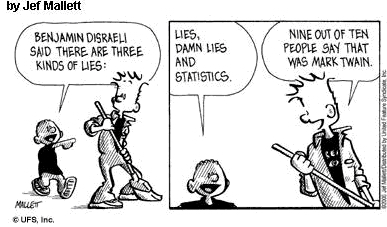
\includegraphics[height=3cm]{../images/StatsLies.jpg} \hspace{1cm} 
\includegraphics[height=3cm]{../images/StatsDodgy2.jpg}

\vspace{.5cm}
But in a data rich world, statistical literacy is essential for everyone, whether in medicine, science, business, education, engineering, marketing or law, as it allows evidence based reasoning. 
\end{frame}


\begin{frame}{}
For example, has the incidence of brain cancer risen in Australia since the introduction of mobile phones 29 years ago? Mobile phone use in Australia has increased rapidly since its introduction in 1987 with whole population usage being 94\% by 2014. There is a popularly hypothesised association between brain cancer incidence and mobile phone use. Is it valid?

\vspace{.5cm}
Or, does public feeling toward sharks grow negative following shark bites on humans? Media and government responses are often predicated on this presumptive emotional response; but how should public policy be developed?

\vspace{.5cm}
Statistics has endless interesting applications and is highly collaborative, as John Wilder Tukey said, 
`The best thing about being a statistician is that you get to play in everyone's backyard.'
\end{frame}

\begin{frame}{}
That's why there are so many jobs for `data scientists'. According to Val Kinsley, Chief economist at Google, `I keep saying the sexy job in the next ten years will be statisticians. People think I'm joking, but who would've guessed that computer engineers would've been the sexy job of the 1990s?' or a recent Fortune magazine, 'The nerdy-cool job that companies are scrambling to fill: data scientist.'

\vspace{.5cm}
\href{https://en.wikipedia.org/wiki/Frazz}{\beamergotobutton{Cartoon1Source}} 
\href{http://vadlo.com/Research_Cartoons/Depends-upon-what-is-more-publishable.gif}{\beamergotobutton{Cartoon2 Source}}
\href{https://flowingdata.com/category/statistics/mistaken-data/}{\beamergotobutton{Mistaken Data}} 
\href{http://www.mckinsey.com/insights/innovation/hal_varian_on_how_the_web_challenges_managers}{\beamergotobutton{McKinsey Article}}  
\href{http://www.careercast.com/jobs-rated/jobs-rated-report-2016-ranking-200-jobs}{\beamergotobutton{2016 Top Jobs}}
\href{www.nytimes.com/2000/07/28/us/john-tukey-85-statistician-coined-the-word-software.html}{\beamergotobutton{Tukey}}
\href{http://www.amadeus.com/blog/18/06/10-reasons-why-data-scientist-is-the-sexiest-job-or-not/}{\beamergotobutton{Data Scientist}}
\href{http://fortune.com/2011/09/06/data-scientist-the-hot-new-gig-in-tech/}{\beamergotobutton{Fortune}}
\end{frame}



\subsection[]{What is Statistics?}
\begin{frame}{What is Statistics?}
\begin{block}{Definition (Statistics)}
Statistics is the science of learning from data. It is problem-solving. We pose questions of data and enable data to pose questions.
\end{block}

\begin{block}{Definition (Big Data)}
Big Data is `inconveniently large data’ (Clair Alston), with characteristics such as high-volume, high-variety, high-velocity, high-variability, high-value and low-veracity.
\end{block}

\begin{block}{Definition (Population and Sample)}
A population is the full amount of information being studied, of which a sample (or data) is a subset.
\end{block}
\end{frame}

\begin{frame}{}

We often only have access to a sample of a population. Why? Hence, the critical question driving much Statistical Research is: What information does the sample give about the population and how reliable is that information?

\begin{center}
\begin{tikzpicture}[very thick, level distance = 2cm,
population/.style={rectangle,draw, fill=blue!20},
sample/.style={rectangle,draw,fill=green!20,rounded corners=.8ex},
  %%every node/.style = {shape=rectangle, rounded corners,
   %% draw, align=center,
   %% top color=white, bottom color=blue!20}
    ]]  
  \node[population, minimum height = 1.5cm, minimum width = 6cm] { Population  }
    child { node[sample] {Sample}   };
\end{tikzpicture}
\end{center}
\end{frame}

%%%% PART 1 %%%%
  \section[Part1]{PART1: EXPLORATORY DATA ANALYSIS (EDA)}
\subsection[]{Overview of Exploraratory Data Analysis (EDA)}
\begin{frame}{Overview of Exploraratory Data Analysis (EDA)}
``What can we learn about the data?" \\

\vspace{.5cm}
Exploratory Data Analysis or Descriptive Statistics is about creating a snapshot or summary of the data. This helps us to identify the data's main qualities, and hence aids us in understanding the population from which it derives.

\begin{center}
\begin{tikzpicture}[very thick, level distance = 2cm,
population/.style={rectangle,draw},
sample/.style={rectangle,draw,fill=green!20,rounded corners=.8ex},
%%every node/.style = {shape=rectangle, rounded corners,
%% draw, align=center,
%% top color=white, bottom color=blue!20}
]]

\node[population, minimum height = 1.5cm, minimum width = 6cm] { Population  }
child { node[sample] {Sample}   };
\end{tikzpicture}
\end{center}
\end{frame}

\begin{frame}{}
\begin{center}
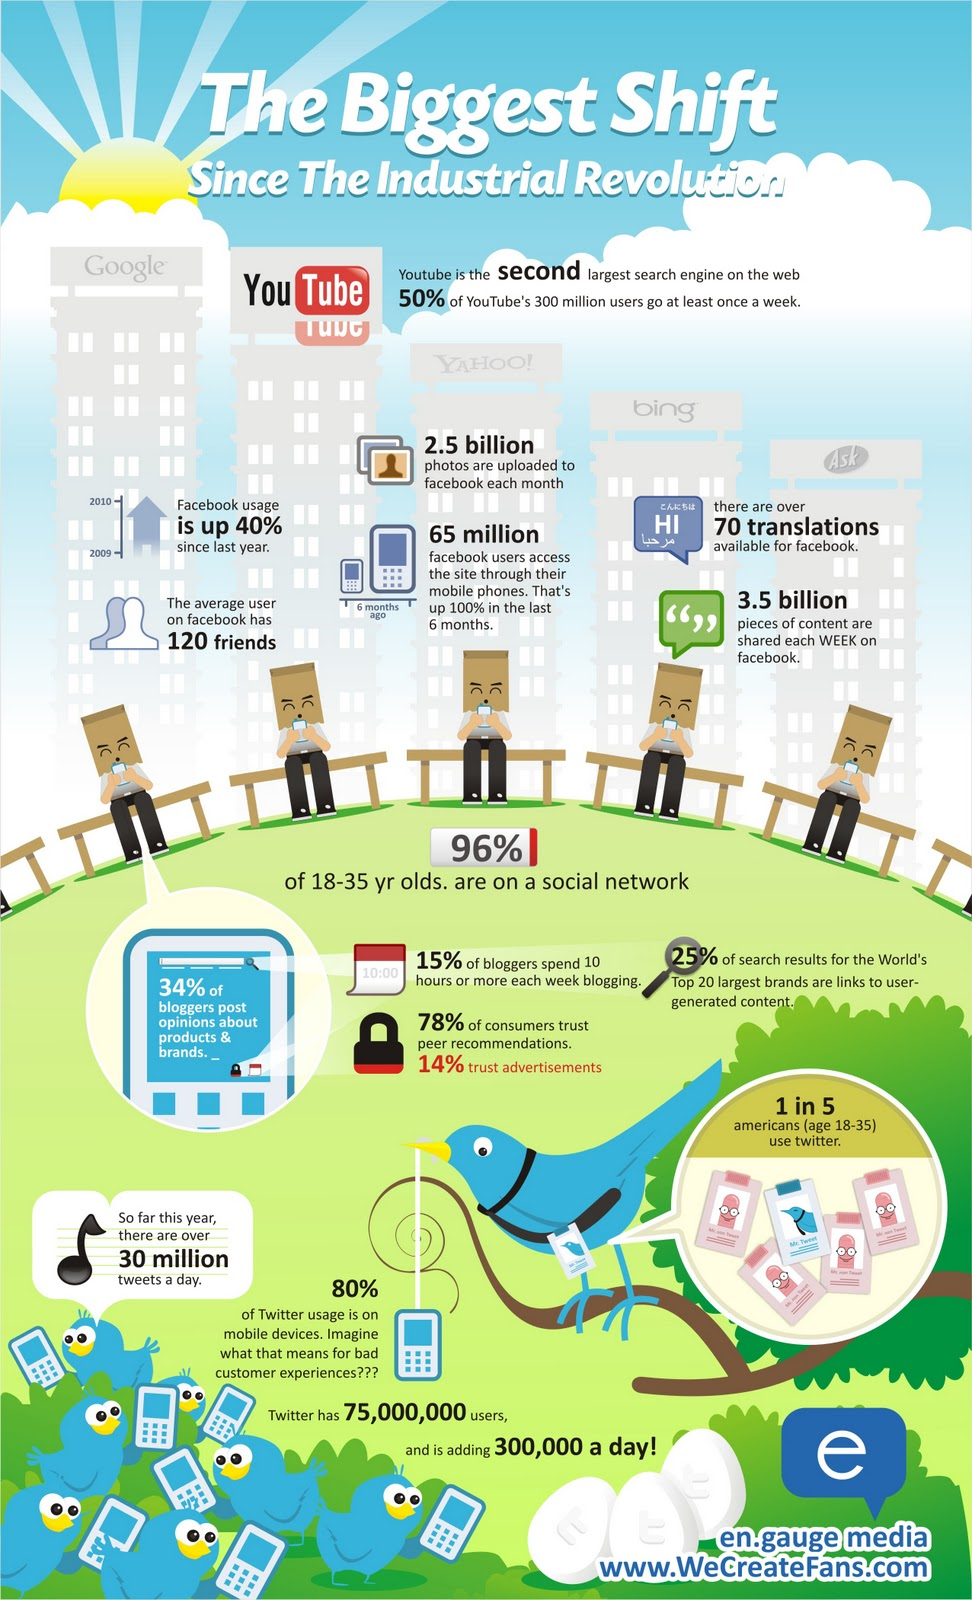
\includegraphics[height=7cm]{../images/SocialMediaStats.jpg}
\end{center}
%\hyperimage{http://www.socialfactor.com/wp-content/uploads/2013/01/Social_Media_Stats.jpg}  %Load image
\href{http://www.socialfactor.com/social-media-the-biggest-shift-since-the-industrial-revolution}{\beamergotobutton{Source}}  %Why not work?
\end{frame}




\section[1]{Topic1: Data and Graphical Summaries}

\subsection[]{Example: Australian Road Fatalities Jan-April 2016}
\begin{frame}{Example: Australian Road Fatalities Jan-April 2016}

The number of road fatalities in Australia continues to rise, given the ever increasing volume of vehicles on the road, despite preventative measures as compulsory seat belts and school zones. Last year in Australia, 1,209 died on our roads.

\vspace{.5cm}
Data from the Australian Bureau of Statistics (ABS) from the first four months of 2016, gives the following variables: \\

Crash ID, State, Date, Day, Month, Year, Dayweek, Time, Hour, Min, Crash Type, Bus Involvement, Rigid Truck Invovement, Articulated Truck Involvement, Speed Limit, Road User, Gender, Age.
\href{http://www.maths.usyd.edu.au/u/UG/JM/StatsData.html}{\beamergotobutton{See DataDictionary}} 

\vspace{.5cm}
{\bf What questions do you have?}
\end{frame}

\subsection[]{Identifying Variables}

\begin{frame}[fragile]{Identifying Variables}

{\tiny
\begin{knitrout}
\definecolor{shadecolor}{rgb}{0.969, 0.969, 0.969}\color{fgcolor}\begin{kframe}
\begin{alltt}
\hlcom{## data <- read.csv("2016Fatalities.csv",header=T)}
\hlstd{data[}\hlnum{1}\hlstd{,]}  \hlcom{#Extracts the 1st row}
\end{alltt}
\begin{verbatim}
##     Crash.ID State     Date Day   Month Year Dayweek  Time Hour Min
## 1 2.2016e+12   VIC 1-Jan-16   1 January 2016  Friday 20:30   20  30
##       Crash.Type BusInvolvement RigidTruck..Involvement
## 1 Single vehicle             No                      No
##   Articulated.Truck..Involvement. SpeedLimit         RoadUser Gender Age
## 1                              No         80 Motorcycle rider   Male  25
\end{verbatim}
\end{kframe}
\end{knitrout}
}

\begin{knitrout}
\definecolor{shadecolor}{rgb}{0.969, 0.969, 0.969}\color{fgcolor}\begin{kframe}
\begin{alltt}
\hlkwd{names}\hlstd{(data)} \hlcom{#Lists all the variables}
\hlkwd{colnames}\hlstd{(data)}  \hlcom{#Lists all the variables}
\hlkwd{head}\hlstd{(data)}  \hlcom{#List the 1st 5 rows of data}
\hlkwd{class}\hlstd{(data)}  \hlcom{#Shows the way R has stored the data}
\end{alltt}
\end{kframe}
\end{knitrout}

\begin{knitrout}
\definecolor{shadecolor}{rgb}{0.969, 0.969, 0.969}\color{fgcolor}\begin{kframe}
\begin{alltt}
\hlkwd{dim}\hlstd{(data)}
\end{alltt}
\begin{verbatim}
## [1] 442  18
\end{verbatim}
\end{kframe}
\end{knitrout}


\end{frame}


\begin{frame}{}
The 1st step in EDA is to identify the variables, in terms of form and type. 

\vspace{.5cm}
{\bf (i) Size of Variables} \\
How many bits of information or ‘variables’ have been recorded? \\
In `big data' we commonly have `large $p$, small $n$' meaning that we have stacks of variables (eg gene data) relative to the data size.

{\tiny \begin{center}
\begin{tikzpicture}[sibling distance=10em,
  every node/.style = {shape=rectangle, rounded corners,
    draw, align=center,
    top color=white, bottom color=blue!20}]]
  \node {Size}
    child { node {Multivariate \\ = 2+ variables}
      child { node {Bivariate \\ = 2 variables} } 
      child { node {Univariate \\ = 1 variable} }};
\end{tikzpicture}
\end{center}}
\end{frame}

\begin{frame}{}

{\bf (ii) Type of Variables} \\
What is the nature of the variables – i.e. what process or situation  ‘produced’ the data?

{\tiny  \begin{center}
\begin{tikzpicture}[level distance = 1.5cm,
level 1/.style={sibling distance=5cm},
level 2/.style={sibling distance=2cm},
  every node/.style = {shape=rectangle, rounded corners,
    draw, align=center,
    top color=white, bottom color=blue!20}]]
  \node {Type}
    child { node {Numerical  or Quantitative \\ = Measurements} 
    child { node {Discrete \\ = Separated \\ Eg Year} }
      child { node {Continuous \\ = Continuum \\ Eg Age} }  }
    child { node {Categorical  or Qualitative \\ = Named, coded categories}
      child { node {Ordinal \\ = Ordered \\ Eg Crash Type}
      child { node {Binary = 2 categories} } 
      }
      child { node {Nominal \\ = Non-Ordered \\ }  
      child { node {Binary \\ Eg Gender} } }};
\end{tikzpicture}
\end{center}}
\end{frame}


\begin{frame}{}
Note:
\begin{itemize}
\item
In practise, continuous data is often reported as discrete data (by rounding), but the underlying quantity represented is still continuous (eg Age and Time).
\item
A helpful diagnostic for determining continuous data is to ask: “Could this data have been recorded to higher accuracy, given a more precise ‘instrument’?”
\item
Quantitative data can be simplified to qualitative data. For example, in a survey, a respondent may feel more comfortable giving a general answer to a question about their personal income.
\end{itemize}
\end{frame}

\begin{frame}
\begin{alertblock}{Have a try}
Identify all the variables for Australian Road Fatalities.
\end{alertblock}

{\tiny  \begin{center}
\begin{tikzpicture}[level distance = 1cm,
level 1/.style={sibling distance=5cm},
level 2/.style={sibling distance=2.5cm},
  every node/.style = {shape=rectangle, rounded corners,
    draw, align=center,
    top color=white, bottom color=blue!20}]]
  \node {Type}
    child { node {Numerical} 
    child { node {Discrete \hspace{1cm} \\    \\ \\ \\ \\} }
      child { node {Continuous \hspace{.5cm} \\ \\ \\ \\ \\ } }  }
    child { node {Categorical}
      child { node {Ordinal \hspace{1cm} \\  \\ \\  \\ \\}
      }
      child { node {Nominal \hspace{1cm}  \\ \\ \\  \\ \\}   }};
\end{tikzpicture}
\end{center}}
\end{frame}


\subsection[]{Graphical Summaries}
\begin{frame}{Graphical Summaries}
Once we identify the variables, we can summarise the data, both graphically and numerically, in order to identify and highlight the main features of interest.   A careful choice of graphical and numerical summaries can give a quick, transparent, perceptive snapshot of the data. 

\vspace{.5cm}
We often start with graphical summaries because `A picture is worth a thousand words.' (Similar idea: Arthur Brisbane, Syracuse Advertising Men's Club, 1911)

\begin{center}
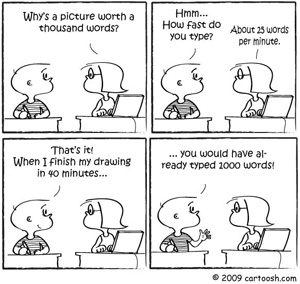
\includegraphics[height=3.5cm]{../images/PictureWords.jpg}
\end{center}
\href{www.abpublish.co.uk/blogphotos/picture_thousand_words.jpg}{\beamergotobutton{Source}}
\end{frame}


\begin{frame}{How to choose an appropriate graphical summary?}
The critical question is: `How can I visually represent this data?' or `What plot will best highlight features of the data?'. This knocks out pie charts and 3D charts!

\vspace{.5cm}
To some extent we use trial and error. We try some standard forms and see what is revealed about the data. One graphical summary can suggest another, and often a combination will highlight different features of the data

\vspace{.5cm}
In practise we use computer packages like R to construct summaries.
However, it is important to understand how to construct graphical summaries ‘by hand’, so that you understand how to interpret computer output and for your final exam. Some computer packages vary slightly in construction. For example, in the calculation of the quartiles or the length of the whiskers in the boxplot.
\end{frame}


\subsection[]{Summary0: Barplot}
\begin{frame}[fragile]{Summary0: Barplot (Categorical data)}

{\bf Q: What was the most common day of road fatality?}

{\tiny 
\begin{knitrout}
\definecolor{shadecolor}{rgb}{0.969, 0.969, 0.969}\color{fgcolor}\begin{kframe}
\begin{alltt}
\hlstd{DayWeek} \hlkwb{<-} \hlstd{data}\hlopt{$}\hlstd{Dayweek}
\hlkwd{table}\hlstd{(DayWeek)}
\end{alltt}
\begin{verbatim}
## DayWeek
##    Friday    Monday  Saturday    Sunday  Thursday   Tuesday Wednesday 
##        68        50        85        56        58        67        58
\end{verbatim}
\begin{alltt}
\hlkwd{plot}\hlstd{(}\hlkwd{table}\hlstd{(DayWeek),}\hlkwc{las}\hlstd{=}\hlnum{2}\hlstd{)}
\end{alltt}
\end{kframe}
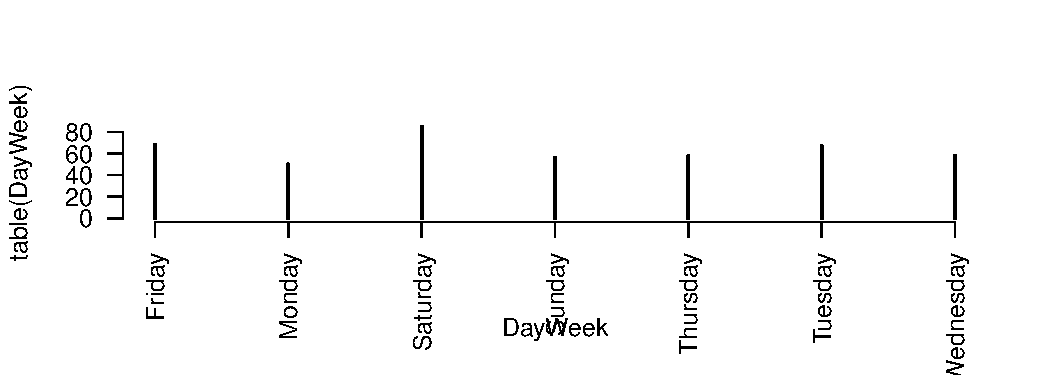
\includegraphics[width=\maxwidth]{figure/unnamed-chunk-7-1} 

\end{knitrout}
}
\end{frame}


\subsection[]{Summary1: Frequency table and ordinate diagram}
\begin{frame}[fragile]{Summary1: Frequency table and ordinate diagram (discrete data)}

{\bf Q: What was the most common speed at which a road fatality occurred?}

\vspace{.5cm}
The frequency table is a very simple way to summarise a set of discrete data and when plotted gives an ordinate diagram. 

\vspace{1cm}
\begin{tabular}{l|llllll|l} \hline
Speed & -9 & 40 & 50 & \ldots & 130 & 888 & Total \\ \hline
Frequency & 28 & 4  & & & &  1 &  442 \\ \hline
\end{tabular}

\vspace{.5cm}
What is strange? Why?
\end{frame}

\begin{frame}[fragile]{}
\begin{knitrout}
\definecolor{shadecolor}{rgb}{0.969, 0.969, 0.969}\color{fgcolor}\begin{kframe}
\begin{alltt}
\hlstd{Speed} \hlkwb{<-} \hlstd{data}\hlopt{$}\hlstd{SpeedLimit}  \hlcom{#Extracts SpeedLimit}
\hlkwd{table}\hlstd{(Speed)}
\end{alltt}
\begin{verbatim}
## Speed
##  -9  40  50  60  70  80  90 100 110 130 888 
##  28   4  53  70  21  53  10 128  71   3   1
\end{verbatim}
\begin{alltt}
\hlkwd{plot}\hlstd{(}\hlkwd{table}\hlstd{(Speed))}
\end{alltt}
\end{kframe}
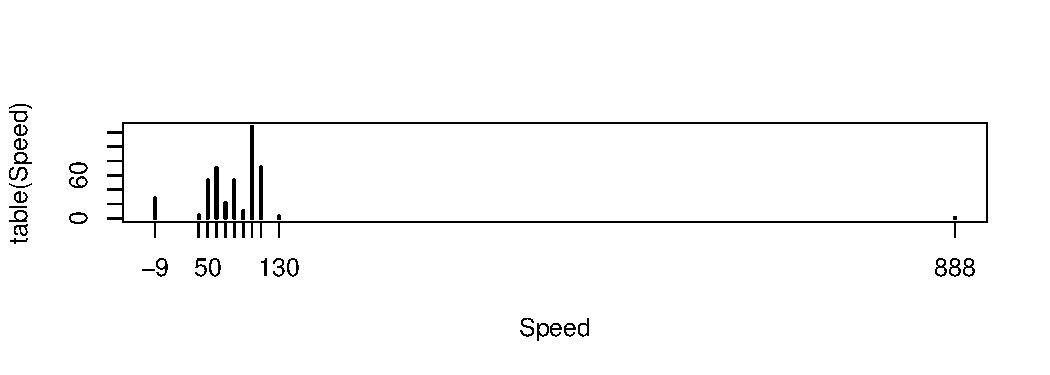
\includegraphics[width=\maxwidth]{figure/unnamed-chunk-8-1} 

\end{knitrout}
\end{frame}

\subsection[]{Summary2: Frequency table and histograms}
\begin{frame}[fragile]{Summary2: Frequency table and histograms (continuous data)}

{\bf Q: What were the most common ages at which a road fatality occurred?}

\vspace{.5cm}
The frequency table can also be used to summarise a set of continuous data, by collecting it into intervals (or ‘bins’). What is lost?

\begin{itemize}
\item 
For equal bin lengths, we can simply sort the data into the bins, and then plot the frequency against each bin. This is called a `regular' histogram. 

\item
For unequal bin lengths, we need to sort the data into the bins, then work out the relative frequency (=frequency/sample size) and the height (=relative frequency/interval length). Plotting the height against each bin is called a 'probability' histogram.
\end{itemize}
\end{frame}

\begin{frame}[fragile]{}

{\bf (i) Using equal bins: Regular Histogram} \\

\begin{center}
\begin{tabular}{| l | l| } \hline
\mbox{Bin} & \mbox{Frequency} \\ \hline
[-10,0) & ? \\ \hline
[0,10) & 11  \\ \hline
[10,20) &  \\ \hline
\ldots &  \\ \hline
[90,100) & 9  \\ \hline
\end{tabular} 
\end{center}

\begin{knitrout}
\definecolor{shadecolor}{rgb}{0.969, 0.969, 0.969}\color{fgcolor}\begin{kframe}
\begin{alltt}
\hlstd{Age} \hlkwb{<-} \hlstd{data}\hlopt{$}\hlstd{Age}
\hlkwd{min}\hlstd{(Age)}
\end{alltt}
\begin{verbatim}
## [1] -9
\end{verbatim}
\begin{alltt}
\hlkwd{max}\hlstd{(Age)}
\end{alltt}
\begin{verbatim}
## [1] 96
\end{verbatim}
\end{kframe}
\end{knitrout}
\end{frame}

\begin{frame}[fragile]{}
\begin{knitrout}
\definecolor{shadecolor}{rgb}{0.969, 0.969, 0.969}\color{fgcolor}\begin{kframe}
\begin{alltt}
\hlstd{Age} \hlkwb{<-} \hlstd{data}\hlopt{$}\hlstd{Age}
\hlkwd{hist}\hlstd{(Age,}\hlkwc{xlab}\hlstd{=}\hlstr{"Age"}\hlstd{,}
     \hlkwc{main}\hlstd{=}\hlstr{"Regular Histogram for Age of Fatality"}\hlstd{)}
\end{alltt}
\end{kframe}
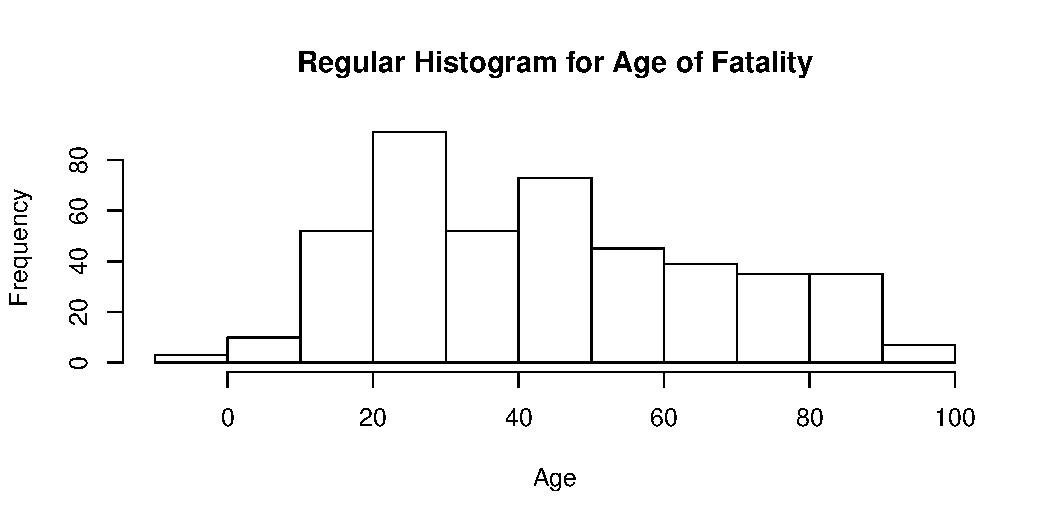
\includegraphics[width=\maxwidth]{figure/unnamed-chunk-10-1} 

\end{knitrout}
\end{frame}

\begin{frame}[fragile]{}

{\bf (ii) Using unequal bins: Probability Histogram} \\

\begin{center}
\begin{tabular}{| l | l| l| l| } \hline
\mbox{Bin} & \mbox{Frequency} & \mbox{Relative Frequency} & \mbox{Height} \\ \hline
[-10,18) & 31  & 31/442 = 0.07 & 0.0025  \\ \hline
[18,25) & 72  & 72/442 = 0.16 & 0.0232 \\ \hline
[25,70) & 259  & 259/442 = 0.59 &  0.0130 \\ \hline
[70,100) & 80  &  80/442 = 0.18 & 0.0060 \\ \hline
Total & 442 & 1 & \\ \hline
\end{tabular} 
\end{center}

where: \\
Relative Frequency = Frequency/442 \\
Height = Relative Frequency/Bin length \\
Eg For bin [-10,18): height = 0.07/28 =3.6. \\
\end{frame}

\begin{frame}[fragile]{}
\begin{knitrout}
\definecolor{shadecolor}{rgb}{0.969, 0.969, 0.969}\color{fgcolor}\begin{kframe}
\begin{alltt}
\hlstd{breaks}\hlkwb{=}\hlkwd{c}\hlstd{(}\hlopt{-}\hlnum{10}\hlstd{,}\hlnum{18}\hlstd{,}\hlnum{25}\hlstd{,}\hlnum{70}\hlstd{,}\hlnum{100}\hlstd{)}
\hlkwd{table}\hlstd{(}\hlkwd{cut}\hlstd{(Age,breaks,}\hlkwc{right}\hlstd{=F))}
\end{alltt}
\begin{verbatim}
## 
## [-10,18)  [18,25)  [25,70) [70,100) 
##       31       72      259       80
\end{verbatim}
\begin{alltt}
\hlkwd{hist}\hlstd{(Age,}\hlkwc{br}\hlstd{=breaks,}\hlkwc{freq}\hlstd{=F,}\hlkwc{right}\hlstd{=F,}
     \hlkwc{xlab}\hlstd{=}\hlstr{"Age"}\hlstd{,}
     \hlkwc{main}\hlstd{=}\hlstr{"Probability Histogram for Age of Fatality"}\hlstd{)}
\end{alltt}
\end{kframe}
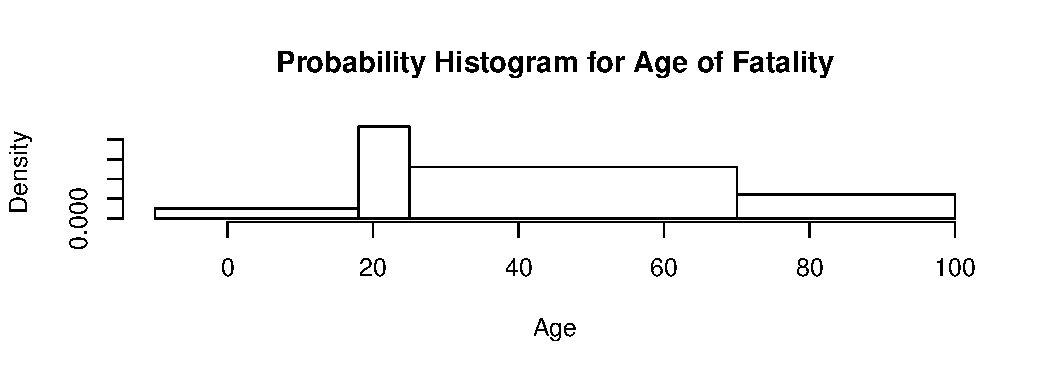
\includegraphics[width=\maxwidth]{figure/unnamed-chunk-11-1} 

\end{knitrout}
\end{frame}

\begin{frame}[fragile]{}
Note how the `regular' histogram is misleading for unequal bin lengths, as it suggests that [25,70) is the most likely bin.

%Gives warning message, hence input pdf following.
%<<fig.height=3,echo=F, results='hide',message=FALSE>>=
%breaks=c(-10,18,25,70,100)
%table(cut(Age,breaks,right=F))   
%hist(Age,br=breaks,freq=T, right=F, main ="Misleading Regular Histogram")  

\vspace{.5cm}
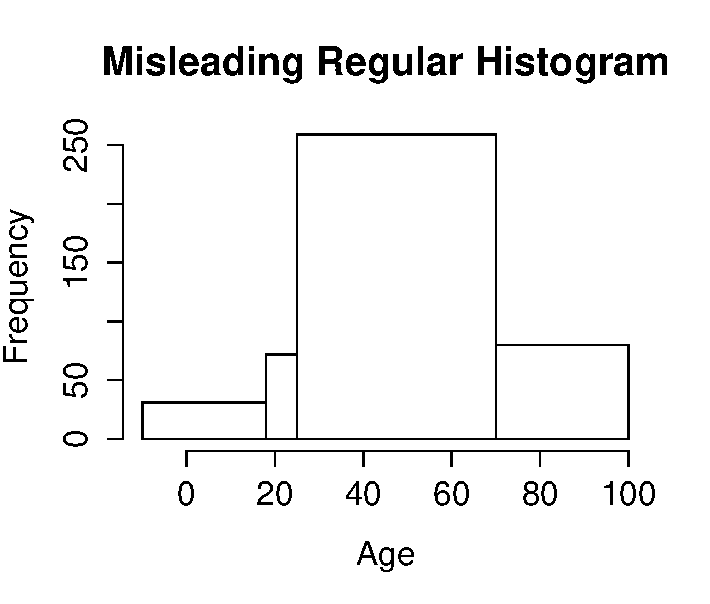
\includegraphics[height=6cm]{../images/AgeMisleadingHist.pdf}
\end{frame}

\subsection[]{Summary3: Stem and leaf plot}
\begin{frame}[fragile]{Summary3: Stem and leaf plot}

{\bf Q: What were the 3 highest ages at which a road fatality occurred?}

\vspace{.5cm}
A stem and leaf plot is basically a histogram turned on its side. It is useful for moderately sized data sets. It provides both a sense of the shape and an ordering of the data, while retaining all the raw numerical data (up to a certain decimal place). 

\vspace{.5cm}
The value to the left of the $\mid$ is called the ‘stem’ and the values on the right are called ‘leaves’.
The leaves should be ordered, although sorting will not affect the shape of the plot.
\end{frame}

\begin{frame}[fragile]{}

{\tiny 
\begin{knitrout}
\definecolor{shadecolor}{rgb}{0.969, 0.969, 0.969}\color{fgcolor}\begin{kframe}
\begin{alltt}
\hlkwd{stem}\hlstd{(Age)}
\end{alltt}
\begin{verbatim}
## 
##   The decimal point is 1 digit(s) to the right of the |
## 
##   -0 | 99
##    0 | 011124557
##    1 | 0034555677777777777788888888888888999999999
##    2 | 00000000000111111222222222223333333333444444444445555555555566666666+12
##    3 | 000000000011111222223333333334445556666666667777778888899
##    4 | 00000111111222222233333333344444444444555555556666666666777777788888
##    5 | 00011111233333344455556777777888888889999
##    6 | 0000000111111122233334445555677788899999999
##    7 | 00011122333444444555556666777788899
##    8 | 000111112222222223333344467788888999
##    9 | 001222336
\end{verbatim}
\end{kframe}
\end{knitrout}
}

Note that R defaults to what it considers to be a sensible layout of the data. Here R chooses a `single' stem plot: with each stem having the leaves 0,1,2,...9. So the reading 2 $\mid$ 3 is age 23. If we consider the data is over-condensed (too stretched out) or under-condensed (too bunched up), we can adjust the format by experimenting with {\tt scale=}.
\end{frame}


\begin{frame}[fragile]{}

{\tiny 
\begin{knitrout}
\definecolor{shadecolor}{rgb}{0.969, 0.969, 0.969}\color{fgcolor}\begin{kframe}
\begin{alltt}
\hlkwd{stem}\hlstd{(Age,}\hlkwc{scale}\hlstd{=}\hlnum{0.25}\hlstd{)}
\end{alltt}
\begin{verbatim}
## 
##   The decimal point is 1 digit(s) to the right of the |
## 
##   -0 | 99
##    0 | 0111245570034555677777777777788888888888888999999999
##    2 | 00000000000111111222222222223333333333444444444445555555555566666666+69
##    4 | 00000111111222222233333333344444444444555555556666666666777777788888+36
##    6 | 00000001111111222333344455556777888999999990001112233344444455555666
##    8 | 000111112222222223333344467788888999001222336
\end{verbatim}
\end{kframe}
\end{knitrout}
}
This is called a double leaf plot, as the stem `0' now has the leaves 0,1,2,3,4 5,6,7,8,9 (representing 00-09) and then a second set of leaves 0,1,2,3,4 5,6,7,8,9 (representing 10-19).  Note you need to read carefully, as 8|0 can represent both 80 or 90.

\vspace{.5cm}
A double stem plot would have one stem `0' with leaves 0,1,2,3,4 (representing 00-04) and then a second stem 'O' with leaves 5,6,7,8,9 (representing 05-09).
\end{frame}

\subsection[]{Summary4: Boxplot}
\begin{frame}[fragile]{Summary4: Boxplot}

\vspace{.5cm}
{\bf Q: Were there any unusual ages at which a road fatality occurred? Is there any difference between the ages of male and female fatalities?}

\vspace{.5cm}
Boxplots are useful for comparing data sets and identifying outliers. 

\begin{knitrout}
\definecolor{shadecolor}{rgb}{0.969, 0.969, 0.969}\color{fgcolor}\begin{kframe}
\begin{alltt}
\hlkwd{boxplot}\hlstd{(Age,}\hlkwc{horizontal}\hlstd{=T)}
\end{alltt}
\end{kframe}
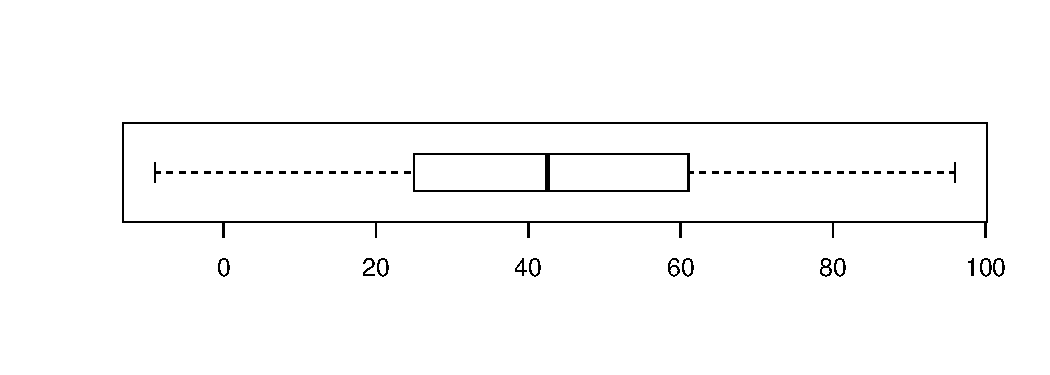
\includegraphics[width=\maxwidth]{figure/unnamed-chunk-14-1} 

\end{knitrout}
 
\end{frame}

\begin{frame}[fragile]{}
\begin{knitrout}
\definecolor{shadecolor}{rgb}{0.969, 0.969, 0.969}\color{fgcolor}\begin{kframe}
\begin{alltt}
\hlstd{AgeM} \hlkwb{<-} \hlstd{data}\hlopt{$}\hlstd{Age[ data}\hlopt{$}\hlstd{Gender} \hlopt{==} \hlstr{"Male"}\hlstd{]}
\hlstd{AgeF} \hlkwb{<-} \hlstd{data}\hlopt{$}\hlstd{Age[ data}\hlopt{$}\hlstd{Gender} \hlopt{==} \hlstr{"Female"}\hlstd{]}
\hlkwd{par}\hlstd{(}\hlkwc{mfrow} \hlstd{=} \hlkwd{c}\hlstd{(}\hlnum{1}\hlstd{,} \hlnum{2}\hlstd{))}  \hlcom{#Puts 2 boxplots in a row}
\hlkwd{boxplot}\hlstd{(AgeM)}
\hlkwd{boxplot}\hlstd{(AgeF)}
\end{alltt}
\end{kframe}
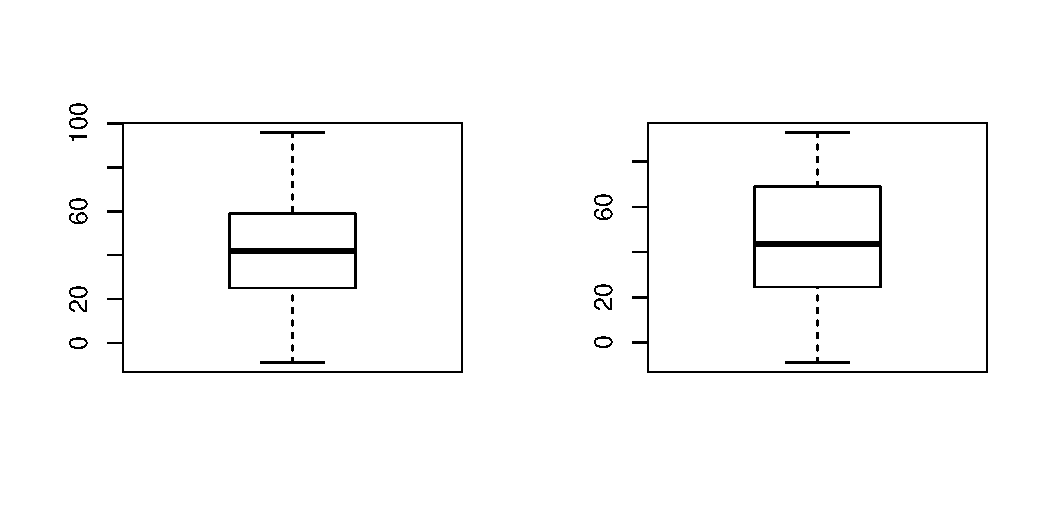
\includegraphics[width=\maxwidth]{figure/unnamed-chunk-15-1} 

\end{knitrout}
\end{frame}

\begin{frame}[fragile]{}

A neat trick for producing the same boxplots:
\begin{knitrout}
\definecolor{shadecolor}{rgb}{0.969, 0.969, 0.969}\color{fgcolor}\begin{kframe}
\begin{alltt}
\hlkwd{boxplot}\hlstd{(Age}\hlopt{~}\hlstd{data}\hlopt{$}\hlstd{Gender,} \hlkwc{ylab}\hlstd{=}\hlstr{"Age"}\hlstd{)}
\end{alltt}
\end{kframe}
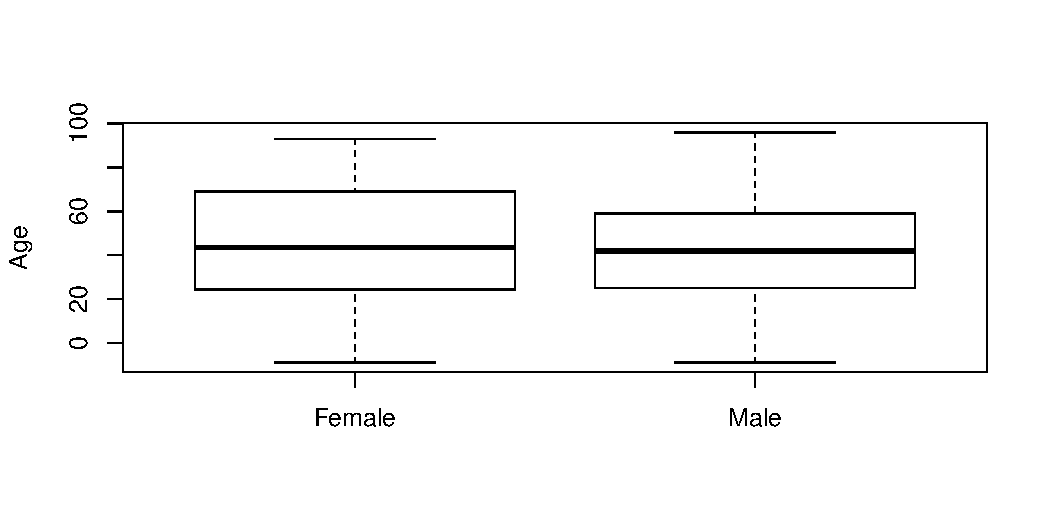
\includegraphics[width=\maxwidth]{figure/unnamed-chunk-16-1} 

\end{knitrout}
\end{frame}


\begin{frame}[fragile]{}

The boxplots show that the ages of road fatalities for men and women is similar.
However, what do we learn from this simple commmand?

\begin{knitrout}
\definecolor{shadecolor}{rgb}{0.969, 0.969, 0.969}\color{fgcolor}\begin{kframe}
\begin{alltt}
\hlkwd{length}\hlstd{(AgeM)}
\end{alltt}
\begin{verbatim}
## [1] 326
\end{verbatim}
\begin{alltt}
\hlkwd{length}\hlstd{(AgeF)}
\end{alltt}
\begin{verbatim}
## [1] 116
\end{verbatim}
\end{kframe}
\end{knitrout}
\end{frame}

\begin{frame}[fragile]{}

{\bf Q: What were there any unusual speeds at which fatalities occurred?}

\begin{knitrout}
\definecolor{shadecolor}{rgb}{0.969, 0.969, 0.969}\color{fgcolor}\begin{kframe}
\begin{alltt}
\hlkwd{boxplot}\hlstd{(data}\hlopt{$}\hlstd{SpeedLimit,} \hlkwc{horizontal} \hlstd{= T)}
\end{alltt}
\end{kframe}
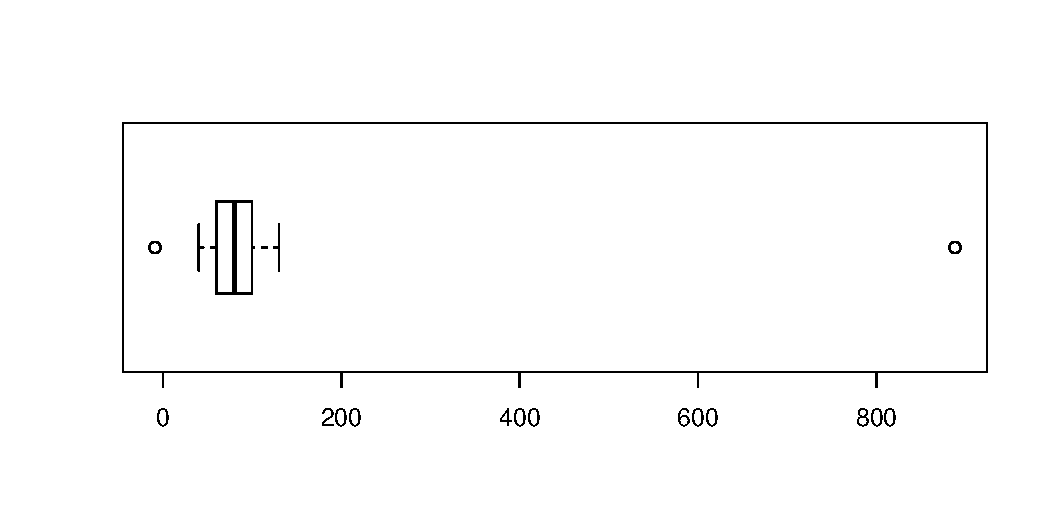
\includegraphics[width=\maxwidth]{figure/unnamed-chunk-18-1} 

\end{knitrout}
\end{frame}

\begin{frame}[fragile]{}
\vspace{.5cm}
A box plot is a visual representation of the 5 number summary
(min, $Q_1$= 1st quartile, $Q_2$= median, $Q_3$= 3rd quartile, max), where:

\begin{itemize}
\item Min = smallest data point(s) \\
\item Max = largest data point(s) \\
\item $Q_2$ = middle data point (find the average of the 2 middle points for even sized dataset.) \\
\item $Q_{1}$ and $Q_{3}$ are the `medians' of the half data sets: we divide the data into 2 sets at the median (including the median for an odd sized data set), and then find the median of each half set of data.
\end{itemize}

See more fuller definitions:  \hyperlink{Quartiles}{\beamergotobutton{Quartiles}} 

\end{frame}


\begin{frame}[fragile]{}

There are different conventions for boxplots. We will use the convention that the whiskers extend to the minimum and maximum observations within the thresholds [LT,UT], where 
\begin{itemize}
\item Lower Threshold $LT=Q_1-1.5IQR$;
\item Upper Threshold $UT=Q_3+ 1.5IQR$;
\item Interquartile range is $IQR=Q_3-Q_1$.
\end{itemize}

\vspace{.5cm}
An outlier is any observation lying outside of [LT,UT].
\end{frame}


\begin{frame}[fragile]{}
\vspace{1cm}
\begin{tikzpicture}[thick, framed]
    \filldraw[fill=green!20] (2,0) rectangle (5,1);% draw the box
    \draw (3,0) -- (3,1) node[above]{$\textsc{Q2}$};% draw the median
    \draw (5,0.5) -- (7,0.5);% draw right whisker
    \draw (2,0.5) -- (1,0.5);% draw left whisker
    \draw (7,0.39) -- (7,0.61);% draw vertical tab
    \draw (1,0.39) -- (1,0.61);% draw vertical tab
    \node[below] at (2,0) {$\textsc{Q1}$};% label the hinge
    \node[below] at (5,0) {$\textsc{Q3}$};% label the hinge
    \filldraw[ball color=red!80,shading=ball] (4,0.5) circle
        (0.06cm) node[above]{$\bar{x}$};% the mean
    \draw[<->] (2.3, -0.3) -- (4.7, -0.3)
        node[pos=0.5,below]{$\textsc{IQR}$}; % mark the IQR fences
    \draw[<->] (2, -0.8) -- (0,-0.8)
        node[pos=0.5,below]{$\textsc{1.5*IQR}$}; % left inner fence
  %  \draw[<->] (2,-1.4) -- (-2, -1.4)
  %      node[pos=0.5,below]{$\textsc{3*IQR}$};% left outer fence
    \draw[<->] (5, -0.8) -- (8,-0.8)
        node[midway,below]{$\textsc{1.5*IQR}$}; % right inner fence
  %  \draw[<->] (5,-1.4) -- (10, -1.4)
   %     node[pos=0.5,below]{$\textsc{3*IQR}$};% right outer fence
    %
  %  \node[below] at (7.5,0.7) {$o$}; % mild outlier on the right
    \node[below] at (0,0.7) {$o$}; % extreme outlier on the left
    % Title
    \draw (3,2) node[above,xshift=0.7cm]{$ \textsc{Box
        Plot}$};%
    % Axis
  %  \draw (-3,-2) -- (8,-2);
    % Note that the snaked line is drawn to 11.1 to force
    % TikZ to draw the final tick.
  %  \draw[snake=ticks,segment length=1cm] (-3,-2) -- (8.1,-2);
\end{tikzpicture}

\vspace{.5cm}
Note: Here we have indicated the mean $\bar{x}$ in red for comparision with the median $Q_{2}$, but normally that is not shown on the boxplot.
\end{frame}

\begin{frame}[fragile]{Steps for Constructing a Boxplot by Hand}
\begin{enumerate}
\item Calculate the quartiles $Q_1$, $Q_2$ and $Q_3$ and the interquartile range $IQR$. 
\item Draw a box from $Q_1$ to $Q_3$, with a line within the box for the median= $Q_2$.
\item Calculate the upper and lower thresholds.
\item Draw a whisker from the box to the nearest points within the thresholds.
\item Any points outside the thresholds are outliers, designated by circles.
\end{enumerate}
\end{frame}

\subsection[]{Describing the Shape of Data}
\begin{frame}[fragile]{Describing the Shape of Data}

When we look at graphical summaries, we want to describe the form of the data and any ‘idiosyncrasies’.

\vspace{.5cm}
3 key questions:

1. Is it symmetric or skewed?
\begin{knitrout}
\definecolor{shadecolor}{rgb}{0.969, 0.969, 0.969}\color{fgcolor}
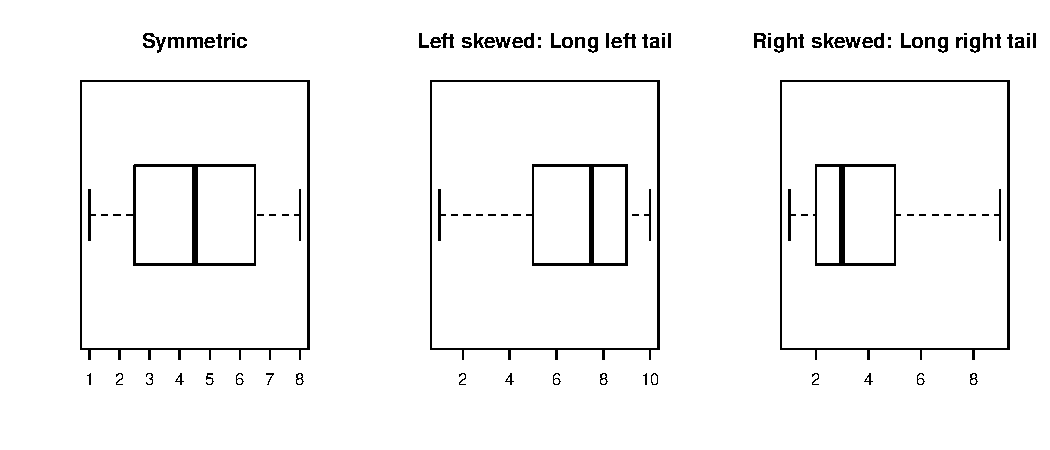
\includegraphics[width=\maxwidth]{figure/unnamed-chunk-19-1} 

\end{knitrout}
\end{frame}

\begin{frame}[fragile]{}

2. Is it unimodal, bimodal, trimodal, multimodal or other?
\begin{knitrout}
\definecolor{shadecolor}{rgb}{0.969, 0.969, 0.969}\color{fgcolor}
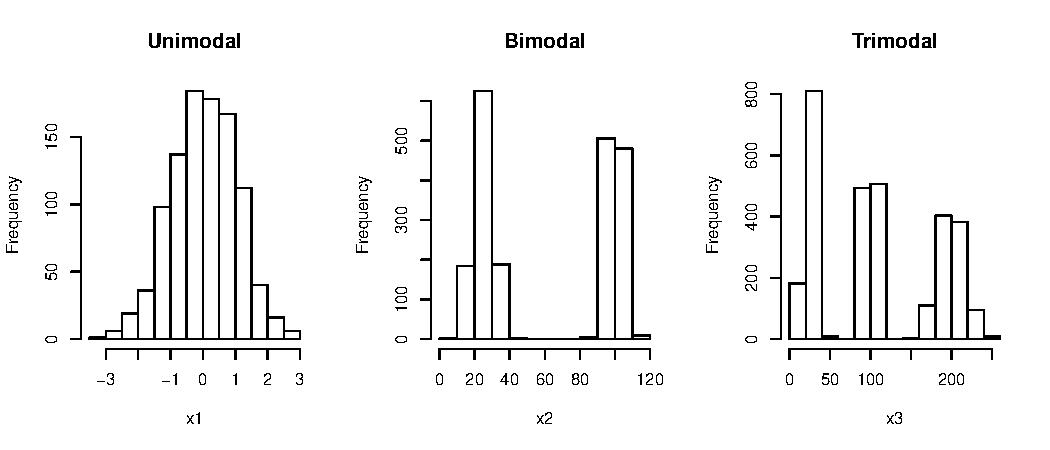
\includegraphics[width=\maxwidth]{figure/unnamed-chunk-20-1} 

\end{knitrout}

Note: Bimodality can be an indication of interesting behaviour to explore. However, it can also arise from 2 populations mistakingly put together. 
\end{frame}

\begin{frame}[fragile]{}

3. Are there any unusual features?  (eg outliers or gaps)
\begin{knitrout}
\definecolor{shadecolor}{rgb}{0.969, 0.969, 0.969}\color{fgcolor}
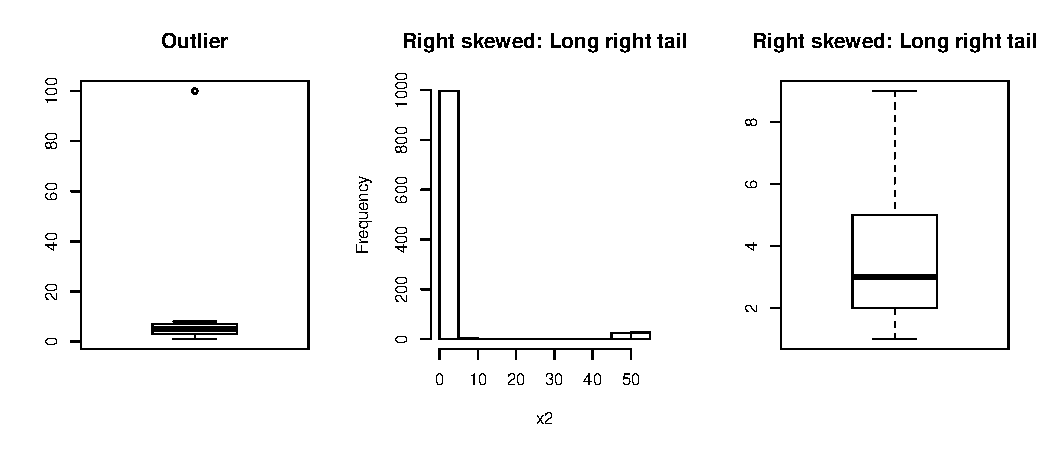
\includegraphics[width=\maxwidth]{figure/unnamed-chunk-21-1} 

\end{knitrout}


Note: An outlier needs to be investigated carefully, as it can be an indication of an interesting data point or possibly a mistake in the recording of data.
\end{frame}


\subsection[]{Dirty Data}
\begin{frame}[fragile]{Dirty Data}

Notice that throughout Topic1 we have deliberately showcased raw data with the missing values coded as '-9'. This is called 'dirty data' and is how real data exists. 

\vspace{.5cm}
Dealing with 'dirty data' is outside the scope of MATH1005, as it can require some sophistication. Ideally, we would replace all the missing values by a blank. However, one possible strategy is to account for the missing values in your histogram: create the bins (-10,0), [0,18] ..., so there is effectively 1 nonsense bin (although it still affects the calculation of frequencies of the other bins.)
\end{frame}










%%% Dataset used in Topic 1


\section[2]{Topic2: Numerical Summaries}

\subsection[]{Example: Australian Road Fatalities Jan-April 2016}

\begin{frame}[fragile]{Example: Australian Road Fatalities Jan-April 2016}

The Australian Road Deaths Database provides basic details of road transport crash fatalities in Australia as reported by the police each month to the State and Territory road safety authorities.

\vspace{.5cm}
Details provided in the database fall into two groups:
(1) the circumstances of the crash, for example, date, location, crash type \\
(2) some details regarding the persons killed, for example, age, gender and road user group.

\vspace{.5cm}
{\bf What is the most common profile of person killed on Australian roads (eg gender, age, time of accident)?}

\vspace{.5cm}
\href{https://bitre.gov.au/statistics/safety/fatal_road_crash_database.aspx}{\beamergotobutton{Australian Road Deaths Database}}
\end{frame}



\subsection[]{Numerical Summaries}
\begin{frame}[fragile]{Numerical Summaries}
\begin{center}
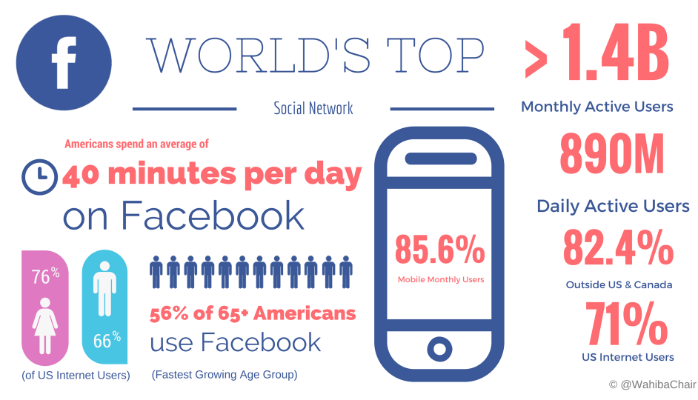
\includegraphics[height=5cm]{../images/SocialMedia2015.png}
\end{center}

A numerical summary describes a certain characteristic of the data in a single value. The notion of a numerical summary is very nice – what is lost in subtlety is gained in simplicity.
For example, in the Australian census data, 1 mean can summarise 21.5 million data points. 
\href{https://www.linkedin.com/pulse/2015-social-media-stats-trends-images-part-1-wahiba-chair-mba}{\beamergotobutton{SocialMediaStats}}
\href{http:\\www.censusdata.abs.gov.au/census_services/getproduct/census/2011/quickstat/0}{\beamergotobutton{AusCensusData}}
\end{frame}

\begin{frame}[fragile]{}

{\bf From the Australian Road Fatalities summaries, what do you learn about the variables?}

{\tiny 
\begin{knitrout}
\definecolor{shadecolor}{rgb}{0.969, 0.969, 0.969}\color{fgcolor}\begin{kframe}
\begin{alltt}
\hlkwd{summary}\hlstd{(data[}\hlnum{1}\hlopt{:}\hlnum{8}\hlstd{])}
\end{alltt}
\begin{verbatim}
##     Crash.ID             State            Date          Day      
##  Min.   :1.202e+12   NSW    :138   17-Apr-16: 10   Min.   : 1.0  
##  1st Qu.:1.202e+12   VIC    :100   20-Feb-16:  9   1st Qu.: 9.0  
##  Median :2.202e+12   QLD    : 76   27-Jan-16:  9   Median :15.0  
##  Mean   :2.973e+12   WA     : 64   5-Mar-16 :  9   Mean   :15.5  
##  3rd Qu.:4.202e+12   SA     : 31   9-Jan-16 :  9   3rd Qu.:22.0  
##  Max.   :8.202e+12   TAS    : 18   16-Feb-16:  8   Max.   :31.0  
##                      (Other): 15   (Other)  :388                 
##       Month          Year           Dayweek        Time    
##  April   :116   Min.   :2016   Friday   :68   13:00  : 10  
##  February:105   1st Qu.:2016   Monday   :50   14:00  : 10  
##  January :106   Median :2016   Saturday :85   21:00  : 10  
##  March   :115   Mean   :2016   Sunday   :56   8:00   : 10  
##                 3rd Qu.:2016   Thursday :58   15:00  :  9  
##                 Max.   :2016   Tuesday  :67   17:00  :  8  
##                                Wednesday:58   (Other):385
\end{verbatim}
\end{kframe}
\end{knitrout}
}
\end{frame}

\begin{frame}[fragile]{}

{\tiny 
\begin{knitrout}
\definecolor{shadecolor}{rgb}{0.969, 0.969, 0.969}\color{fgcolor}\begin{kframe}
\begin{alltt}
\hlkwd{summary}\hlstd{(data[}\hlnum{9}\hlopt{:}\hlnum{18}\hlstd{])}
\end{alltt}
\begin{verbatim}
##       Hour            Min                   Crash.Type  BusInvolvement
##  Min.   : 0.00   Min.   : 0.00   Multiple vehicle:195   No :434       
##  1st Qu.: 8.00   1st Qu.: 0.00   Pedestrian      : 51   Yes:  8       
##  Median :13.00   Median :20.00   Single vehicle  :196                 
##  Mean   :12.52   Mean   :20.84                                        
##  3rd Qu.:17.00   3rd Qu.:35.00                                        
##  Max.   :23.00   Max.   :59.00                                        
##  RigidTruck..Involvement Articulated.Truck..Involvement.   SpeedLimit    
##  No :412                 No :408                         Min.   : -9.00  
##  Yes: 30                 Yes: 34                         1st Qu.: 60.00  
##                                                          Median : 80.00  
##                                                          Mean   : 79.76  
##                                                          3rd Qu.:100.00  
##                                                          Max.   :888.00  
##                                     RoadUser      Gender         Age      
##  Bicyclist (includes pillion passengers): 16   Female:116   Min.   :-9.0  
##  Driver                                 :212   Male  :326   1st Qu.:25.0  
##  Motorcycle pillion passenger           :  4                Median :42.5  
##  Motorcycle rider                       : 89                Mean   :44.6  
##  Passenger                              : 66                3rd Qu.:61.0  
##  Pedestrian                             : 55                Max.   :96.0
\end{verbatim}
\end{kframe}
\end{knitrout}
}
\end{frame}

\begin{frame}[fragile]{}
Note: We use different summaries for different types of variables.  \\

\begin{itemize}
\item {\bf Categorial Data} \\
Categorical data is essentially already summarised by category. We note the most common category or any trend within the categories. \\

\vspace{.5cm}
\item
{\bf Numerical Data} \\
Numerical summaries focus on a feature of interest, like the centre and spread.
\end{itemize}
\end{frame}


\subsection[]{Numerical Data - Notation}
\begin{frame}{Notation for Numerical Summaries}
Given a univariate data set of sample size $n$:

\begin{itemize}
\item
the data is $ \{ x_i \},i=1,2,\ldots,n$   or  $\{ x_{1},x_{2} \ldots, ,x_{n} \}$. 

\vspace{.5cm}
\item the ordered (ascending) data set is $ \{ x_{(i)} \},i=1,2,\ldots,n$ or 
$\{ x_{(1)},x_{(2)},\ldots,x_{(n)} \}$.

\vspace{.5cm}
\item 
the sum of the data is $\sum_{i=1}^{n} x_i = x_1+ x_2+\ldots x_n$.
\end{itemize}
\end{frame}

\begin{frame}[fragile]{}
\begin{alertblock}{Have a try}
Given a data set $\{ 1,4,6,2,3,7\}$, find
\[ \sum_{i=1}^{6} x_{i},  \sum_{i=2}^{5} x_{i}^2, \sum_{i=1}^{6} i x_{i}, \sum_{i=1}^{6} (x_{(i)}-1) \]
\end{alertblock}

\begin{knitrout}
\definecolor{shadecolor}{rgb}{0.969, 0.969, 0.969}\color{fgcolor}\begin{kframe}
\begin{alltt}
\hlcom{#Check your answers}
\hlstd{x}\hlkwb{=}\hlkwd{c}\hlstd{(}\hlnum{1}\hlstd{,}\hlnum{4}\hlstd{,}\hlnum{6}\hlstd{,}\hlnum{2}\hlstd{,}\hlnum{3}\hlstd{,}\hlnum{7}\hlstd{)}
\hlstd{y}\hlkwb{=}\hlkwd{c}\hlstd{(}\hlkwd{sum}\hlstd{(x),} \hlkwd{sum}\hlstd{(x[}\hlnum{2}\hlopt{:}\hlnum{5}\hlstd{]}\hlopt{^}\hlnum{2}\hlstd{),} \hlkwd{sum}\hlstd{(}\hlkwd{c}\hlstd{(}\hlnum{1}\hlopt{:}\hlnum{6}\hlstd{)}\hlopt{*}\hlstd{x),} \hlkwd{sum}\hlstd{(}\hlkwd{sort}\hlstd{(x)}\hlopt{-}\hlnum{1}\hlstd{))}
\hlstd{y}
\end{alltt}
\begin{verbatim}
## [1] 23 65 92 17
\end{verbatim}
\end{kframe}
\end{knitrout}
\href{www.mathsisfun.com/algebra/sigma-notation.html}{\beamergotobutton{More practise here}}
\end{frame}


\subsection[]{Numerical Data - Summaries for Centre}
\begin{frame}[fragile]{Numerical Data - Summaries for Centre}
%[label=SummariesCentre]

There are 2 main measures of the centre (or location) of the data:

\begin{itemize}
\item {\bf Mean} $\bar{x}$ \\
The mean is the average of the data. \\
\[ \bar{x} = \frac{1}{n} \sum_{i=1}^{n} x_{i} \]

\item {\bf Median} $\tilde{x}$ \\
The median is the centre of the data, also called the 50\% percentile or the 2nd quartile. It splits the data into 2 equal groups.  

\begin{itemize}
\item 
If $n$ is odd, the unique median is the middle value:
\[  \tilde{x} = x_{(\frac{n+1}{2})}  \]

\item
If $n$ is even, the median is the average of the 2 middle values (by convention):
\[ \tilde{x} = \frac{x_{(\frac{n}{2})} + x_{(\frac{n}{2} + 1)}}{2} \]
\end{itemize}
\end{itemize}
\end{frame}

\begin{frame}[fragile]{}

\vspace{.5cm}
\begin{alertblock}{Have a try}
For the data: $\{ 1,4,6,2,3,7\}$, show that the mean is 3.83 and the median is 3.5. 
\end{alertblock}

\begin{knitrout}
\definecolor{shadecolor}{rgb}{0.969, 0.969, 0.969}\color{fgcolor}\begin{kframe}
\begin{alltt}
\hlcom{#Check your answers}
\hlstd{x}\hlkwb{=}\hlkwd{c}\hlstd{(}\hlnum{1}\hlstd{,}\hlnum{4}\hlstd{,}\hlnum{6}\hlstd{,}\hlnum{2}\hlstd{,}\hlnum{3}\hlstd{,}\hlnum{7}\hlstd{)}
\hlkwd{mean}\hlstd{(x)}
\end{alltt}
\begin{verbatim}
## [1] 3.833333
\end{verbatim}
\begin{alltt}
\hlkwd{median}\hlstd{(x)}
\end{alltt}
\begin{verbatim}
## [1] 3.5
\end{verbatim}
\end{kframe}
\end{knitrout}

%%%%Extention%%%%
%Note: Data sets which have the same values in the same proportions have the same median (replication principle). For example, the sets $\{ 1,2,3,4 \}$ and $\{ 1,1,1,2,2,2,3,3,3,4,4,4 \}$ have the same median.
\end{frame}


\begin{frame}{Comparing the Mean and Median}
\begin{itemize}
\item 
For symmetric data, we expect $\bar{x} = \tilde{x}$. For left skewed data, we expect $\bar{x} < \tilde{x}$ and for right skewed data, $\bar{x} > \tilde{x}$.
\end{itemize}

\begin{knitrout}
\definecolor{shadecolor}{rgb}{0.969, 0.969, 0.969}\color{fgcolor}
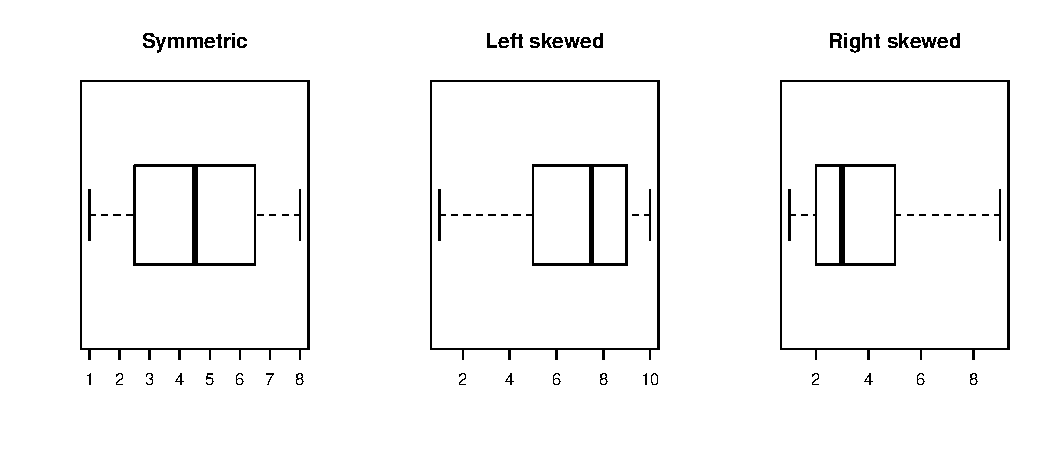
\includegraphics[width=\maxwidth]{figure/unnamed-chunk-28-1} 

\end{knitrout}
\end{frame}


\begin{frame}
\begin{itemize}
\item
Which is ‘optimal’ for describing the centre of the data? 

\vspace{.5cm}
Both have strengths and weaknesses depending on the nature of the data. 
\begin{itemize}
\item Sometimes neither gives a sensible sense of location, for example if the data is bimodal.
\item The median is robust which means it is not affected by some extreme readings. This makes the median preferable for data which is skewed or has many outliers (eg Sydney house prices). 
\item The mean is helpful for data which is basically symmetric which not too many outliers, and for theoretical analysis.
\end{itemize}
\end{itemize}
\end{frame}

\begin{frame}[fragile]{}
\begin{knitrout}
\definecolor{shadecolor}{rgb}{0.969, 0.969, 0.969}\color{fgcolor}\begin{kframe}
\begin{alltt}
\hlstd{Speed} \hlkwb{<-} \hlstd{data}\hlopt{$}\hlstd{SpeedLimit}
\hlkwd{mean}\hlstd{(Speed)}
\end{alltt}
\begin{verbatim}
## [1] 79.76471
\end{verbatim}
\begin{alltt}
\hlkwd{median}\hlstd{(Speed)}
\end{alltt}
\begin{verbatim}
## [1] 80
\end{verbatim}
\begin{alltt}
\hlkwd{par}\hlstd{(}\hlkwc{mfrow} \hlstd{=} \hlkwd{c}\hlstd{(}\hlnum{1}\hlstd{,} \hlnum{2}\hlstd{))}
\hlkwd{boxplot}\hlstd{(Speed,} \hlkwc{horizontal}\hlstd{=T)}
\hlkwd{hist}\hlstd{(Speed)}
\end{alltt}
\end{kframe}
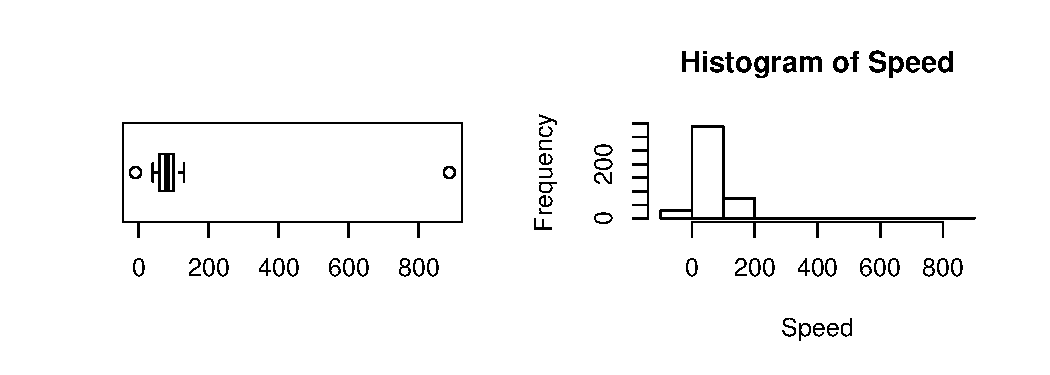
\includegraphics[width=\maxwidth]{figure/unnamed-chunk-29-1} 

\end{knitrout}
\end{frame}


\subsection[]{Numerical Summaries for Spread}
\begin{frame}[fragile]{Numerical Data - Summaries for Spread}
Having summarised the centre of the data, we now want to couple this with a summary of the spread of the data: how far is the data from the centre? The combination of both a numerical centre of centre and spread is a surprisingly helpful snapshot of the data.

\vspace{.5cm}
We can base our summaries for spread on the mean or the quantiles.
\end{frame}

\begin{frame}[fragile]{Spread - based on the Mean (Standard Deviation)}

There are 3 main measures of spread based on the mean:
\begin{itemize}
\item {\bf Mean Absolute Deviation (MAD)}
\[ MAD = \frac{1}{n} \sum_{i=1}^{n} | x_{i} - \bar{x} | \]
This is messy algebraically.

\vspace{.5cm}
\item {\bf Mean Square Error (MSE)}
\[ MSE = \frac{1}{n} \sum_{i=1}^{n} (x_{i} - \bar{x})^2 \]
This requires that we sample $\bar{x}$ from the sample before calculating the MSE: only $n-1$ of the observations are independent of each other.
\end{itemize}
\end{frame}

\begin{frame}[fragile]{}
\begin{itemize}
\item {\bf Standard deviation (SD)}
\[ s= \sqrt{\frac{1}{n-1}  \sum_{i=1}^{n} (x_{i} - \bar{x})^2 } \]

This is called the definition formula: it represents the average of the squared deviations from the mean $\{ (x_{i} - \bar{x}) \}$. We need squared deviations as $\sum_{i=1}^{n} (x_{i} - \bar{x}) = 0$.

\vspace{.5cm}
The calculation formula is
\[ s= \sqrt{\frac{1}{n-1} \big[ \sum_{i=1}^{n} x_{i}^2 - \frac{1}{n} (\sum_{i=1}^{n} x_{i})^2 \big] }
= \sqrt{ \frac{1}{n-1} \big[ \sum_{i=1}^{n} x_{i}^2 - n \bar{x}^2} \big]
\]

\vspace{.5cm}
$s^2 = \frac{1}{n-1} \sum_{i=1}^{n-1} (x_{i} - \bar{x})^2$ is called the variance. 
\end{itemize}
\end{frame}

\begin{frame}[fragile]{Using the Standard Deviation}
Note that $s$ has the same units as $\bar{x}$, so we can couple $(\bar{x}, s)$ as a summary of centre and spread.

\vspace{.5cm}
\begin{block}{Calculating Standard Deviation}
Given $\{ 1,4,6,2,3,7\}$ with $\bar{x}=23/6$, what is the standard deviation? \\

Definition formula: $s= \sqrt{ \frac{1}{5} [ (1-23/6)^2 + (4-23/6)^2 + \ldots (7-23/6)^2 ]} \approx 2.32 $ \\

Calculation formula: $s = \sqrt{ \frac{1}{5} [ 1^2 + 4^2 + 6^2 + 2^2 + 3^2 + 7^2 - 6(23/6)^2] }  \approx 2.32 $

\end{block}

\begin{knitrout}
\definecolor{shadecolor}{rgb}{0.969, 0.969, 0.969}\color{fgcolor}\begin{kframe}
\begin{alltt}
\hlkwd{sd}\hlstd{(x)}
\end{alltt}
\begin{verbatim}
## [1] 2.316607
\end{verbatim}
\end{kframe}
\end{knitrout}
\end{frame}
 
 
 
\begin{frame}[fragile]{}
\begin{knitrout}
\definecolor{shadecolor}{rgb}{0.969, 0.969, 0.969}\color{fgcolor}\begin{kframe}
\begin{alltt}
\hlstd{Speed} \hlkwb{<-} \hlstd{data}\hlopt{$}\hlstd{SpeedLimit}
\hlkwd{mean}\hlstd{(Speed)}
\end{alltt}
\begin{verbatim}
## [1] 79.76471
\end{verbatim}
\begin{alltt}
\hlkwd{median}\hlstd{(Speed)}
\end{alltt}
\begin{verbatim}
## [1] 80
\end{verbatim}
\begin{alltt}
\hlkwd{sd}\hlstd{(Speed)}
\end{alltt}
\begin{verbatim}
## [1] 49.54275
\end{verbatim}
\begin{alltt}
\hlstd{iqr}\hlkwb{=}\hlkwd{fivenum}\hlstd{(Speed)[}\hlnum{4}\hlstd{]}\hlopt{-}\hlkwd{fivenum}\hlstd{(Speed)[}\hlnum{2}\hlstd{]}
\hlstd{iqr}
\end{alltt}
\begin{verbatim}
## [1] 40
\end{verbatim}
\end{kframe}
\end{knitrout}
\end{frame}

\begin{frame}[fragile]{}
\begin{knitrout}
\definecolor{shadecolor}{rgb}{0.969, 0.969, 0.969}\color{fgcolor}\begin{kframe}
\begin{alltt}
\hlkwd{fivenum}\hlstd{(Speed)}
\end{alltt}
\begin{verbatim}
## [1]  -9  60  80 100 888
\end{verbatim}
\begin{alltt}
\hlkwd{boxplot}\hlstd{(Speed,} \hlkwc{horizontal}\hlstd{=T)}
\end{alltt}
\end{kframe}
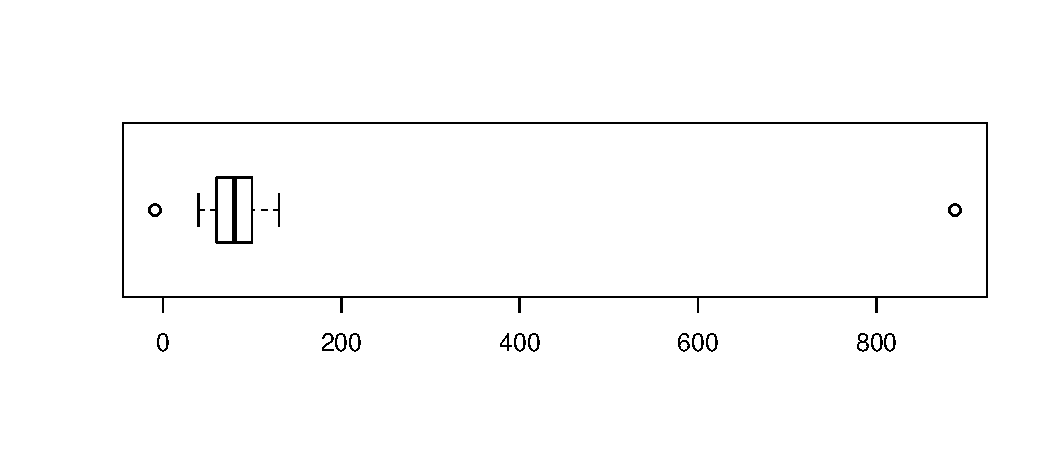
\includegraphics[width=\maxwidth]{figure/unnamed-chunk-32-1} 

\end{knitrout}
\end{frame}
 
 
 
 
\begin{frame}[fragile,label=Quartiles]{Spread - based on the Quartiles (IQR)}
The quartiles are a set of 3 values $\{ Q_{1}, Q_{2} = \tilde{x}, Q_{3} \}$ that roughly split the data into quarters.

\vspace{.5cm}
There is no universal way to define quartiles.  
We use the following convention: we divide the data into 2 sets at the median (including the median for an odd sized data set), and then find the median of each half set of data.

\vspace{.5cm}
Once we have found $Q_{1}$, we can find $Q_{3}$ by symmetry, by counting back from the end of sorted data set.
\end{frame}


\begin{frame}[fragile]{}
\begin{block}{Calculating the Quartiles (even sized sample)}
Given $\{ 1,4,6,2,3,7\}$, the sorted data is $\{ 1,2,3,4,6,7 \}$ and the median $Q_{2} = 3.5$ splits the data into $\{ 1,2,3 \}$ and $\{ 4,6,7 \}$, hence $Q_{1} = 2$ and $Q_{3} = 6$.
\end{block}

\begin{knitrout}
\definecolor{shadecolor}{rgb}{0.969, 0.969, 0.969}\color{fgcolor}\begin{kframe}
\begin{alltt}
\hlcom{# Finds min, Q1, Q2, Q3, max}
\hlkwd{fivenum}\hlstd{(x)}
\end{alltt}
\begin{verbatim}
## [1] 1.0 2.0 3.5 6.0 7.0
\end{verbatim}
\end{kframe}
\end{knitrout}
\end{frame}

\begin{frame}[fragile]{}
\begin{block}{Calculating the Quartiles (even sized sample)}
Given $\{ 1,4,6,2,3,7\}$, the sorted data is $\{ 1,2,3,4,6,7 \}$ and the median $Q_{2} = 3.5$ splits the data into $\{ 1,2,3 \}$ and $\{ 4,6,7 \}$, hence $Q_{1} = 2$ and $Q_{3} = 6$.
\end{block}

\begin{knitrout}
\definecolor{shadecolor}{rgb}{0.969, 0.969, 0.969}\color{fgcolor}\begin{kframe}
\begin{alltt}
\hlcom{# Finds min, Q1, Q2, Q3, max}
\hlkwd{fivenum}\hlstd{(x)}
\end{alltt}
\begin{verbatim}
## [1] 1.0 2.0 3.5 6.0 7.0
\end{verbatim}
\end{kframe}
\end{knitrout}
\end{frame}

\begin{frame}[fragile]{}
\begin{block}{Calculating the Quartiles (odd sized sample)}
Given $\{ 1,4,6,2,3,7,8\}$, the sorted data is $\{ 1,2,3,4,6,7,8 \}$ and the median $Q_{2} = 4$ splits the data into $\{ 1,2,3,4 \}$ and $\{ 4,6,7,8 \}$, hence $Q_{1} = 2.5$ and $Q_{3} = 6.5$.
\end{block}

\begin{knitrout}
\definecolor{shadecolor}{rgb}{0.969, 0.969, 0.969}\color{fgcolor}\begin{kframe}
\begin{alltt}
\hlstd{x2}\hlkwb{=}\hlkwd{c}\hlstd{(}\hlnum{1}\hlstd{,}\hlnum{4}\hlstd{,}\hlnum{6}\hlstd{,}\hlnum{2}\hlstd{,}\hlnum{3}\hlstd{,}\hlnum{7}\hlstd{,}\hlnum{8}\hlstd{)}
\hlkwd{fivenum}\hlstd{(x2)}
\end{alltt}
\begin{verbatim}
## [1] 1.0 2.5 4.0 6.5 8.0
\end{verbatim}
\end{kframe}
\end{knitrout}
\end{frame}


\begin{frame}[fragile]{Interquartile Range (IQR)}
The full range of the data is $x_{(n)} - x_{(1)}$, but this ignores $n-2$ data points.

\vspace{.5cm}
The Interquartile Range is defined as
\[ IQR = Q_{3} -Q_{1} \]
and represents the range of the middle 50\% of the data. 

\vspace{.5cm}
We couple $(\tilde{x}, IQR)$ as a summary of centre and spread.
\begin{knitrout}
\definecolor{shadecolor}{rgb}{0.969, 0.969, 0.969}\color{fgcolor}\begin{kframe}
\begin{alltt}
\hlkwd{fivenum}\hlstd{(x)[}\hlnum{4}\hlstd{]}\hlopt{-}\hlkwd{fivenum}\hlstd{(x)[}\hlnum{2}\hlstd{]}   \hlcom{# Don't use iqr()}
\end{alltt}
\begin{verbatim}
## [1] 4
\end{verbatim}
\end{kframe}
\end{knitrout}
\end{frame}

\begin{frame}[fragile]{The Five Number Summary}
The five number summary is a neat way to summarise the data
\[ ( x_{(1)}, Q_{1}, Q_{2}, Q_{3}, x_{(n)} ) \]
and is essentially drawn by the boxplot.

\begin{knitrout}
\definecolor{shadecolor}{rgb}{0.969, 0.969, 0.969}\color{fgcolor}\begin{kframe}
\begin{alltt}
\hlkwd{fivenum}\hlstd{(x)}
\end{alltt}
\begin{verbatim}
## [1] 1.0 2.0 3.5 6.0 7.0
\end{verbatim}
\begin{alltt}
\hlkwd{boxplot}\hlstd{(x,} \hlkwc{horizontal}\hlstd{=T,} \hlkwc{col}\hlstd{=}\hlstr{"purple"}\hlstd{)}
\end{alltt}
\end{kframe}
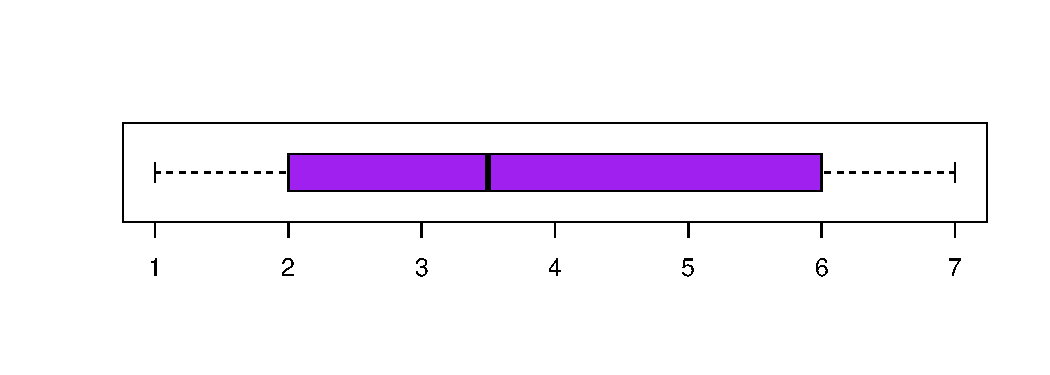
\includegraphics[width=\maxwidth]{figure/unnamed-chunk-37-1} 

\end{knitrout}
\end{frame}

\begin{frame}[fragile]{Comparing the SD and the IQR}
Like the mean and median, the IQR is robust and so preferable for data which is skewed or has many outliers. However, the standard deviation is good for theoretical analysis.

\vspace{.5cm}
\begin{block}{Comparing the SD and the IQR}
Given $\{ 1,4,6,2,3,7,100\}$, what is the sd and IQR?
\end{block}

\begin{knitrout}
\definecolor{shadecolor}{rgb}{0.969, 0.969, 0.969}\color{fgcolor}\begin{kframe}
\begin{alltt}
\hlstd{x1}\hlkwb{=}\hlkwd{c}\hlstd{(}\hlnum{1}\hlstd{,}\hlnum{4}\hlstd{,}\hlnum{6}\hlstd{,}\hlnum{2}\hlstd{,}\hlnum{3}\hlstd{,}\hlnum{7}\hlstd{,}\hlnum{100}\hlstd{)}
\hlkwd{sd}\hlstd{(x1)}
\end{alltt}
\begin{verbatim}
## [1] 36.40905
\end{verbatim}
\begin{alltt}
\hlkwd{fivenum}\hlstd{(x1)[}\hlnum{4}\hlstd{]} \hlopt{-} \hlkwd{fivenum}\hlstd{(x1)[}\hlnum{2}\hlstd{]}
\end{alltt}
\begin{verbatim}
## [1] 4
\end{verbatim}
\end{kframe}
\end{knitrout}
\end{frame}

\subsection[]{Outliers}
\begin{frame}[fragile]{Identifying Outliers}
Outliers are `unusual values' that do not fit the model. They can either indicate interesting values that need futher investigation or a transformation of the model, or they can indicate a possible mistake in your data.

\vspace{.5cm}
There are 2 main ways to identify outliers:
\begin{itemize}
\item {\bf The IQR method (Tukey)} \\
As outlined in the boxplot, we calculate the lower and upper thresholds
\[ LT = Q_{1} - 1.5 IQR  \mbox{  and   }  UT = Q_{3} + 1.5 IQR  \]
Any data point lying outside these thresholds is deemed an outlier. \\
Disadvantages:  No outliers detected for $n \leq 4$ and for large samples wrongly identifies outliers.
\end{itemize}
\end{frame}

\begin{frame}[fragile]{Identifying Outliers}
\begin{itemize}
\item {\bf (Extension: The 3-$\sigma$ method)} \\
Any data point lying more than 3 standard deviations away from the mean is deemed to be an outlier. \\
\[ x_{i} \mbox{ is an outlier iff } |x_{i} - \bar{x}| > 3 \sigma  \]
Disadvantages:  No outliers detected for $n \leq 7$ and for large samples wrongly identifies outliers. \\

\vspace{.5cm}
Note: The 3-sigma edit rule is popular in economics, but it should be avoided in practice due to the following inflexibility, which will make more sense after Part2 of the course. 
\end{itemize}
\end{frame}

\begin{frame}[fragile]{}
The 3-$\sigma$ rule assumes that the underlying distribution is the Normal, and is based on both the sample mean and standard deviation. Problems can occur when either:

\vspace{.5cm}
1) The data is sufficiently skewed. In this case, the mean is no longer a `good' measure of central tendency, and defining outliers as points outside of some symmetric neighbourhood of the mean is not appropriate. The risk is that the `outliers' are detected near the mode rather than the longer tail. Tukey's five number approach is less likely to suffer from this.  
\end{frame}

\begin{frame}[fragile]{}
2) The underlying population has heavy tails. The principle behind the 3-$\sigma$ rule is that $P(  |x_{i} - \bar{x}| > 3 \sigma)$ occurs with small probability, for example when the population is Normal this probability is 0.0027. 

\begin{knitrout}
\definecolor{shadecolor}{rgb}{0.969, 0.969, 0.969}\color{fgcolor}\begin{kframe}
\begin{alltt}
\hlnum{2}\hlopt{*}\hlstd{(}\hlnum{1}\hlopt{-}\hlkwd{pnorm}\hlstd{(}\hlnum{3}\hlstd{))}
\end{alltt}
\begin{verbatim}
## [1] 0.002699796
\end{verbatim}
\end{kframe}
\end{knitrout}

\vspace{.5cm}
If there are heavy tails then this probability can be substantially larger. For example, the probability is 0.029 when the population is $t_{3}$, or 0.10 when the population is $t_{1}$. In the latter case 10\% of the observations will be deemed `outliers'!

%{\tiny 
%<<>>=
%2*(1-pt(3*sqrt(3),3))
%2*(1-pt(3*sqrt(2),1))
%@
%}

\end{frame}


\begin{frame}[fragile]{}
\begin{block}{Detecting Outlier in Data with Mistake}
Suppose we made a mistake in the data entry with heights:
1.68 1.58 1.64 1.73 1.60 1.62 1.78 1.69 1.80 1.74 1.71 1.59 1.63 1.77 1.70 1.77 1.63 1.62 1.80 1.70 1.60 1.77 1.79 1.65 1.66 1.60 1.71 {\bf 178}
\end{block}

IQR method
\begin{knitrout}
\definecolor{shadecolor}{rgb}{0.969, 0.969, 0.969}\color{fgcolor}\begin{kframe}
\begin{alltt}
\hlcom{## Usyd <- read.csv("USyd.csv")}
\hlstd{heights1}\hlkwb{=}\hlkwd{c}\hlstd{(Usyd}\hlopt{$}\hlstd{Heights[}\hlnum{1}\hlopt{:}\hlnum{27}\hlstd{],}\hlnum{178}\hlstd{)}
\hlstd{iqr}\hlkwb{=}\hlkwd{fivenum}\hlstd{(heights1)[}\hlnum{4}\hlstd{]}\hlopt{-}\hlkwd{fivenum}\hlstd{(heights1)[}\hlnum{2}\hlstd{]}
\hlstd{lt}\hlkwb{=}\hlkwd{fivenum}\hlstd{(heights1)[}\hlnum{2}\hlstd{]}\hlopt{-}\hlnum{1.5}\hlopt{*}\hlstd{iqr}
\hlstd{ut}\hlkwb{=}\hlkwd{fivenum}\hlstd{(heights1)[}\hlnum{4}\hlstd{]}\hlopt{+}\hlnum{1.5}\hlopt{*}\hlstd{iqr}
\hlstd{heights1[(heights1}\hlopt{<}\hlstd{lt)} \hlopt{|} \hlstd{(heights1} \hlopt{>} \hlstd{ut)]}   \hlcom{# | = 'or'}
\end{alltt}
\begin{verbatim}
## [1] 178
\end{verbatim}
\end{kframe}
\end{knitrout}
\end{frame}

\begin{frame}[fragile]{}
3-$\sigma$ method
\begin{knitrout}
\definecolor{shadecolor}{rgb}{0.969, 0.969, 0.969}\color{fgcolor}\begin{kframe}
\begin{alltt}
\hlnum{3}\hlopt{*}\hlkwd{sd}\hlstd{(heights1)}
\end{alltt}
\begin{verbatim}
## [1] 99.95986
\end{verbatim}
\begin{alltt}
\hlstd{heights1[}\hlkwd{abs}\hlstd{(heights1}\hlopt{-}\hlkwd{mean}\hlstd{(heights1))}\hlopt{>}\hlnum{3}\hlopt{*}\hlkwd{sd}\hlstd{(heights1)]}
\end{alltt}
\begin{verbatim}
## [1] 178
\end{verbatim}
\end{kframe}
\end{knitrout}
\end{frame}


\begin{frame}[fragile]{Dealing with Outliers by Transformation}
Sometimes an outlier indicates that a better model is needed.
\begin{knitrout}
\definecolor{shadecolor}{rgb}{0.969, 0.969, 0.969}\color{fgcolor}\begin{kframe}
\begin{alltt}
\hlstd{w}\hlkwb{=}\hlkwd{c}\hlstd{(}\hlnum{1}\hlstd{,}\hlnum{2}\hlstd{,}\hlnum{3}\hlstd{,}\hlnum{4}\hlstd{,}\hlnum{10}\hlstd{,}\hlnum{30}\hlstd{,}\hlnum{60}\hlstd{,}\hlnum{120}\hlstd{,}\hlnum{180}\hlstd{,}\hlnum{300}\hlstd{)}
\hlstd{w1}\hlkwb{=}\hlkwd{log}\hlstd{(w,}\hlnum{10}\hlstd{)}
\hlkwd{par}\hlstd{(}\hlkwc{mfrow} \hlstd{=} \hlkwd{c}\hlstd{(}\hlnum{1}\hlstd{,} \hlnum{2}\hlstd{))}
\hlkwd{boxplot}\hlstd{(w,} \hlkwc{main} \hlstd{=}\hlstr{"Data"}\hlstd{)}
\hlkwd{boxplot}\hlstd{(w1,} \hlkwc{main}\hlstd{=}\hlstr{"Log of Data"}\hlstd{)}
\end{alltt}
\end{kframe}
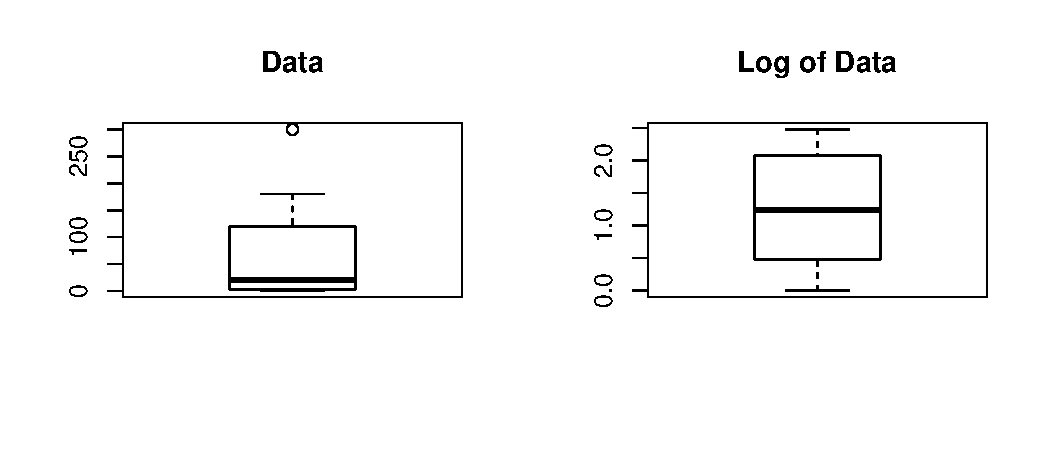
\includegraphics[width=\maxwidth]{figure/unnamed-chunk-42-1} 

\end{knitrout}
\end{frame}





%%% TOPIC3 %%%%
\section[3]{Topic3: Bivariate Data}

\subsection[]{Example: Male Olympic 100m sprints}
\begin{frame}[fragile]{Example: Male Olympic 100m sprints}

The Male 100 metres sprint race in the Olympics is one of the most prestigious events in Athletics. The reigning champion is often named `the fastest man in the world', currently the Jamaican Usain Bolt. 

\vspace{.5cm}
{\bf Are the times getting faster in each Olympics? What would you predict the time for the next Olympics?}

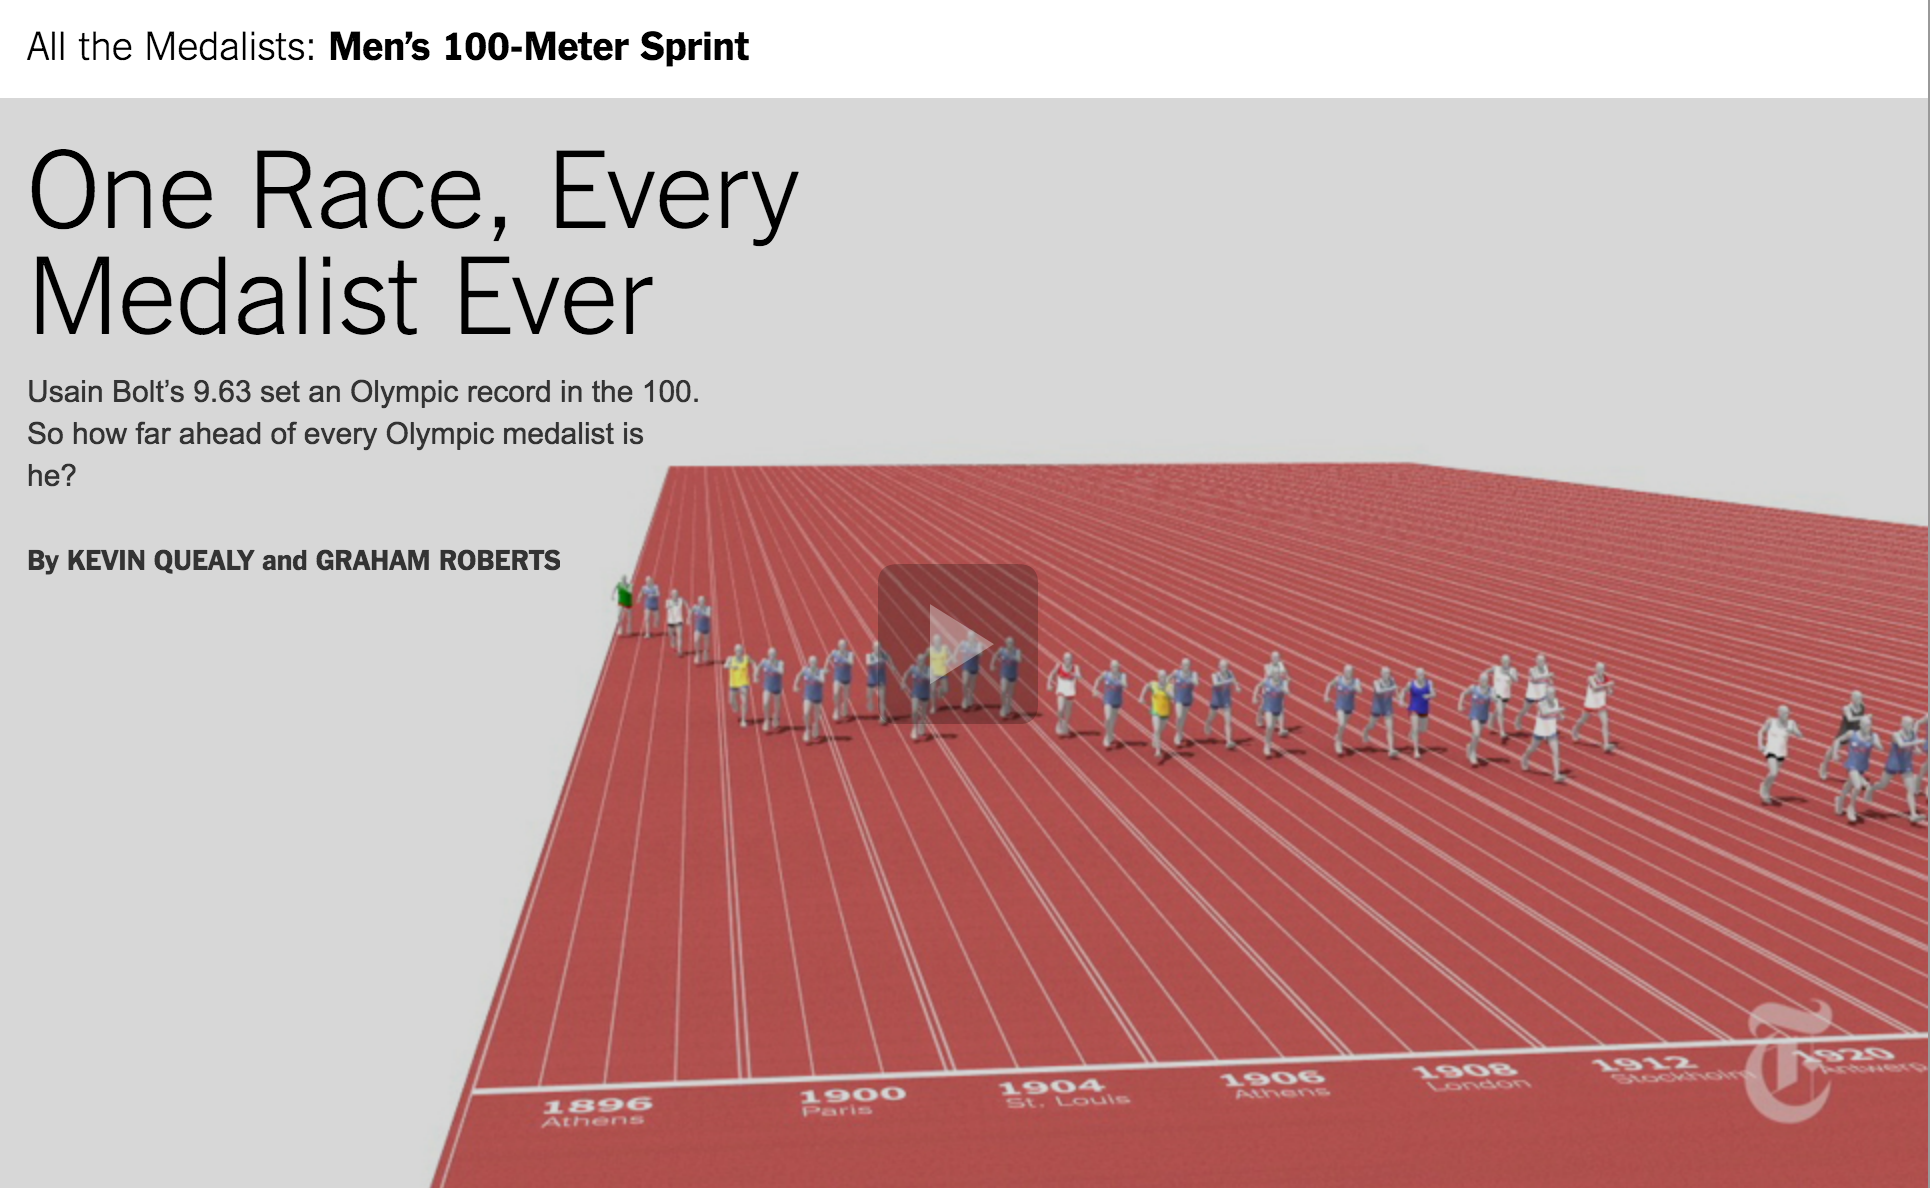
\includegraphics[height=3cm]{../images/Olympics100m.jpg}
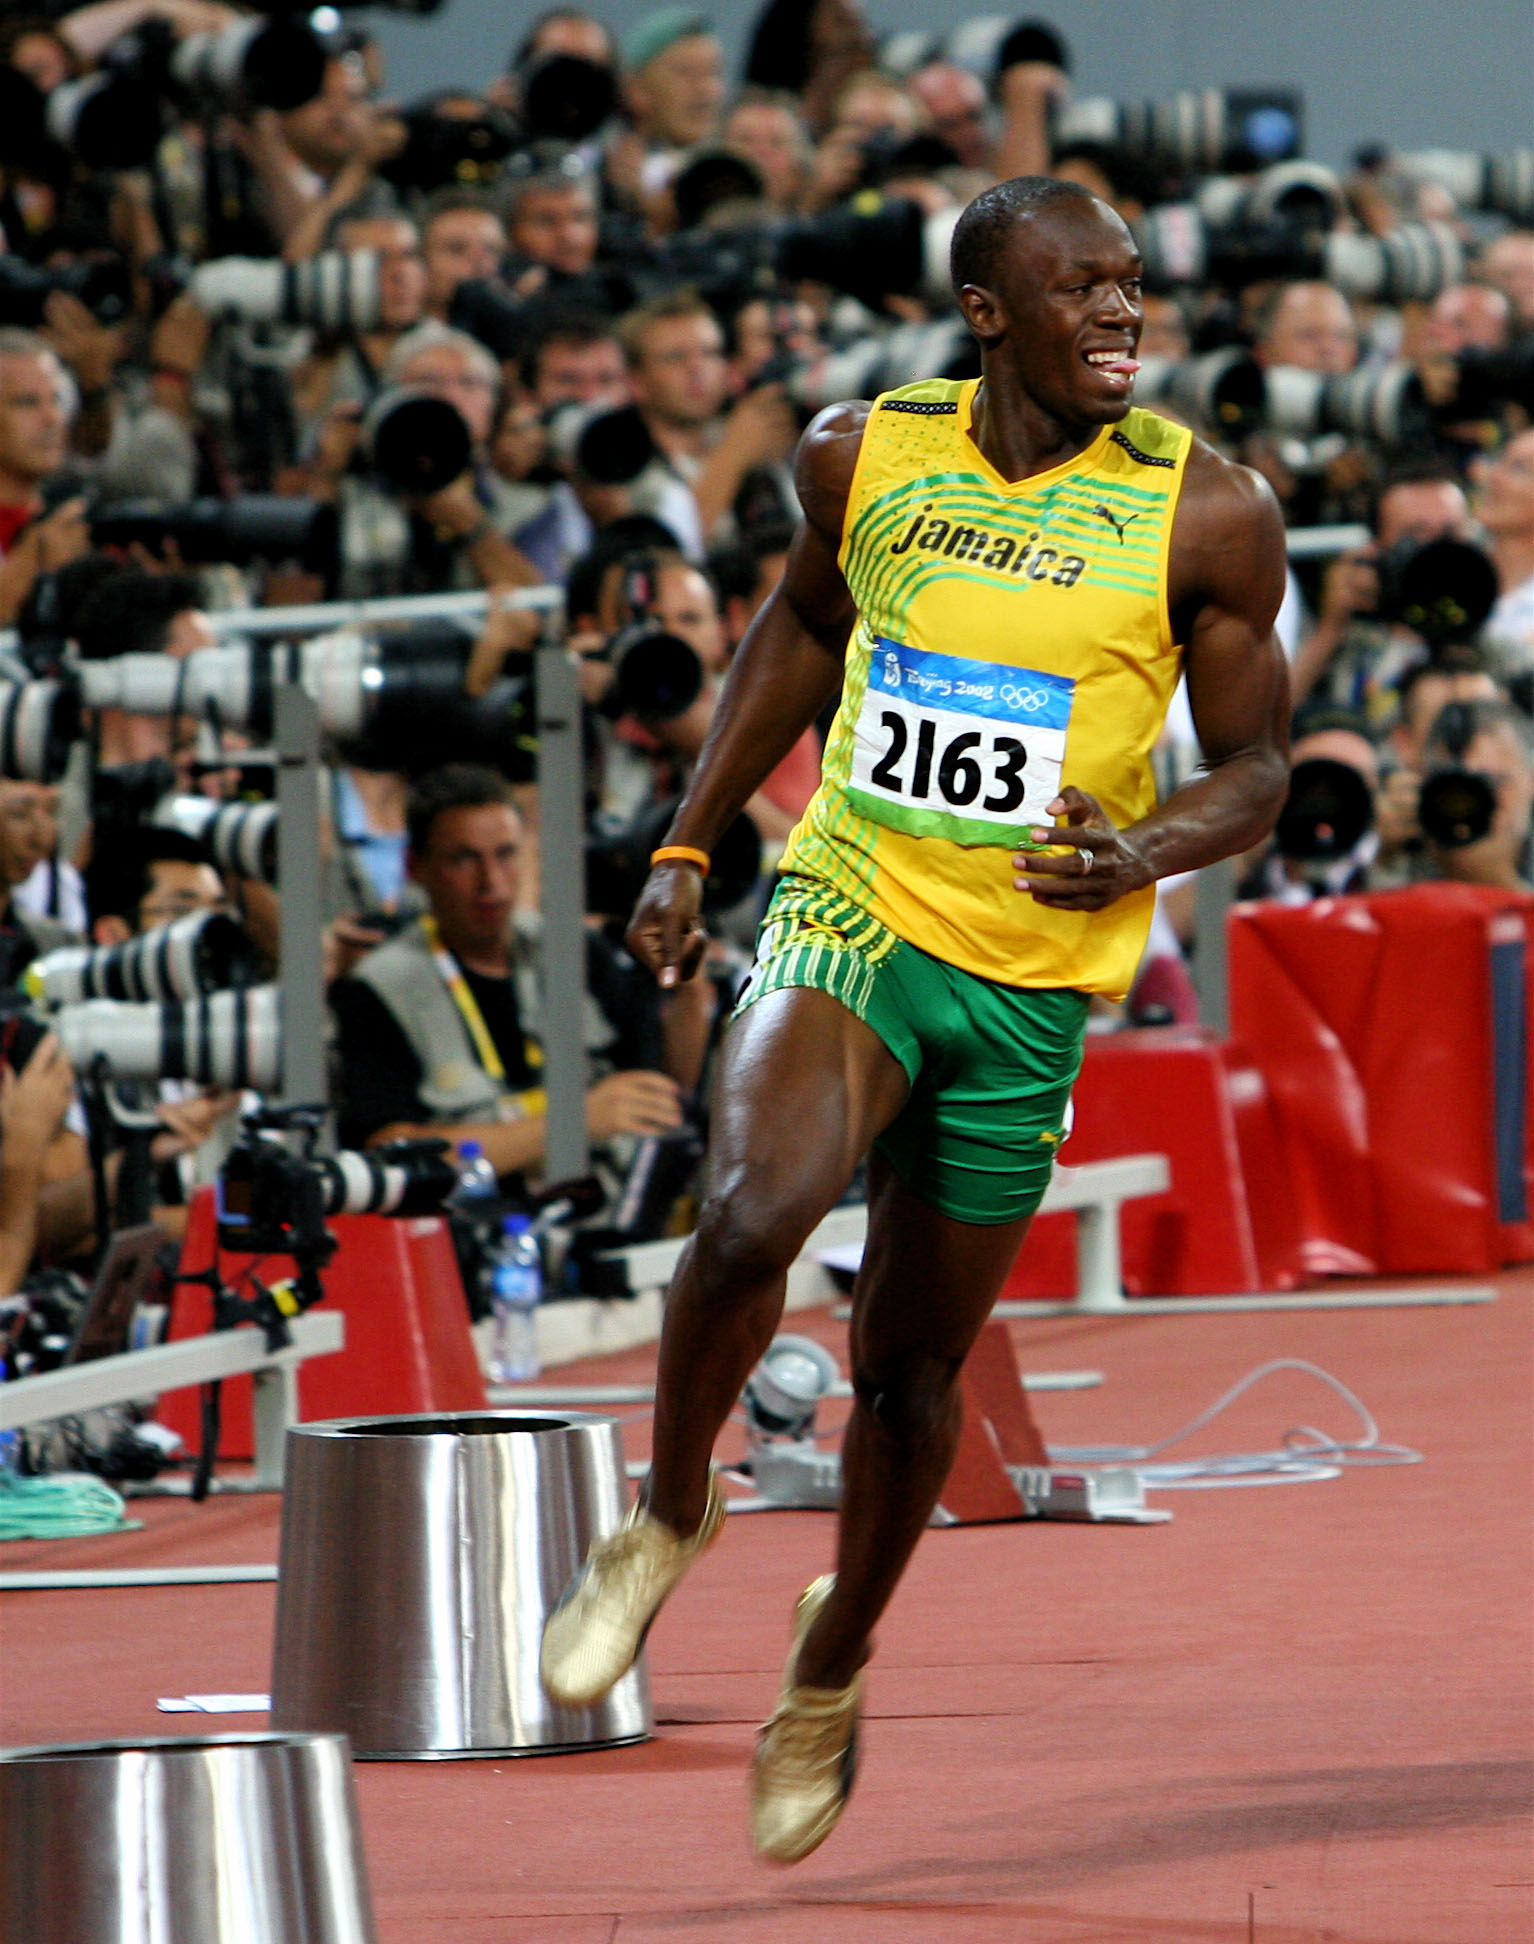
\includegraphics[height=5cm]{../images/UsainBolt.jpg}

\href{http://www.nytimes.com/interactive/2012/08/05/sports/olympics/the-100-meter-dash-one-race-every-medalist-ever.html}{\beamergotobutton{Olympics100mData}}
\end{frame}

\subsection[]{Bivariate Data}
\begin{frame}[fragile]{Bivariate Data}
In most contexts we collect many pieces of information for each ‘individual’ in the data set and look at the relationships between the variables (eg age, height, weight and income for USyd students).  This is called multivariate data.

\begin{itemize}
\item
We just consider bivariate data, of the form: $\{ (x_i,y_i) \}$ for  $i=1,2, \ldots, n$.

\item
$X$ is called the independent variable (or explanatory variable, predictor or regressor) and $Y$ is called the dependent variable (or response variable). These are determined by the context of the data.
\end{itemize}
\end{frame}

\subsection[]{Fitting a Least Squares Regression Model}
\begin{frame}[fragile]{Fitting a Model}
We are interested in fitting a model $Y = f(X) + error$, where the error is independent of the function $f(X)$ and follows a Normal curve (See Topic 6).

\begin{itemize}
\item
Examples include
$Y = \alpha + (X+\beta)^2 + \gamma + error$ (quadratic) or $Y=\alpha e^{\beta X}$ (exponential) or $Y=\alpha X^{\beta}$ (allometric).

\item
We will just consider the linear model: $Y = \alpha + \beta X + error$. 

\item
We use the sample values $\{ (x,y) \}$ to find an estimate of the model:
$y = a + b x + residual$.

\item
Note that both the exponential and allometric models can be expressed as a linear model by taking logs of each side.
\end{itemize}
\end{frame}



\begin{frame}[fragile]{Fitting a Linear Regression (LSL)}
Consider the following 5 steps:  
\begin{enumerate}

\item 
Construct a Scatterplot: $y$ vs $x$.

\item
If the plot looks linear, fit the Least Square’s (Regression) Line (LSL): $\hat{y} = a + b x$. 

\item
Construct a residual plot: $res= y-\hat{y} = y-(a+bx)$ vs $x$

\item
If the residual plot looks random, calculate the coefficient of determination ($r^2$) and correlation coefficient ($r$).

\item
Work out predictions for $y$, by finding $\hat{y}$ for a certain given $x$.
\end{enumerate}
\end{frame}


\subsection[]{Step1: Construct a Scatter plot}
\begin{frame}[fragile]{Step1: Construct a Scatter plot}
The 1st step is to construct a scatterplot of $Y$ vs $X$. This is a graphical summary of the bivariate data.

\vspace{.5cm}
This is 1st diagnostic: does the plot suggest a linear relationship between $Y$ and $X$, or not?
\end{frame}

\begin{frame}[fragile]{}
\begin{knitrout}
\definecolor{shadecolor}{rgb}{0.969, 0.969, 0.969}\color{fgcolor}\begin{kframe}
\begin{alltt}
\hlcom{## olympics <- read.csv("Olympics100m.csv",header=T)}
\hlstd{year}\hlkwb{=}\hlkwd{c}\hlstd{(olympics}\hlopt{$}\hlstd{Year)}
\hlstd{time}\hlkwb{=}\hlkwd{c}\hlstd{(olympics}\hlopt{$}\hlstd{Time)}
\hlkwd{plot}\hlstd{(year,time,} \hlkwc{xlab}\hlstd{=}\hlstr{"year"}\hlstd{,} \hlkwc{ylab}\hlstd{=}\hlstr{"time"}\hlstd{,}
     \hlkwc{main}\hlstd{=}\hlstr{"Olympics 100m 1968-2012"}\hlstd{)}
\end{alltt}
\end{kframe}
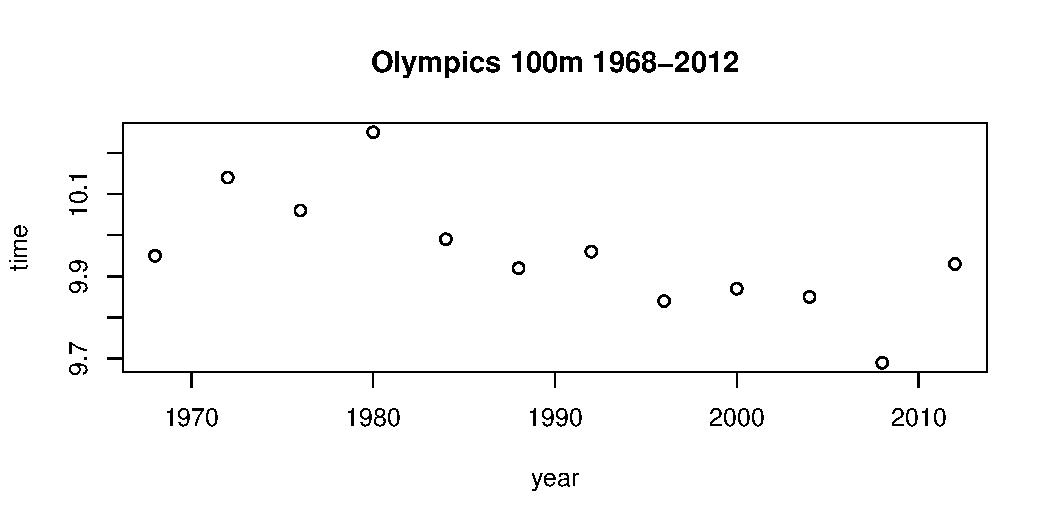
\includegraphics[width=\maxwidth]{figure/unnamed-chunk-44-1} 

\end{knitrout}
\end{frame}


\subsection[]{Step2: Fit the Least Square’s Line (LSL)}
\begin{frame}[fragile]{Step2: Fit the Least Square’s Line (LSL)}
If the scatter plot looks linear, then we fit the Least Square’s Regression Line (LSL).

\begin{itemize}
\item By `eye’, there are many possible lines, which could be drawn on the scatter plot – but which one is optimal?

\begin{knitrout}
\definecolor{shadecolor}{rgb}{0.969, 0.969, 0.969}\color{fgcolor}
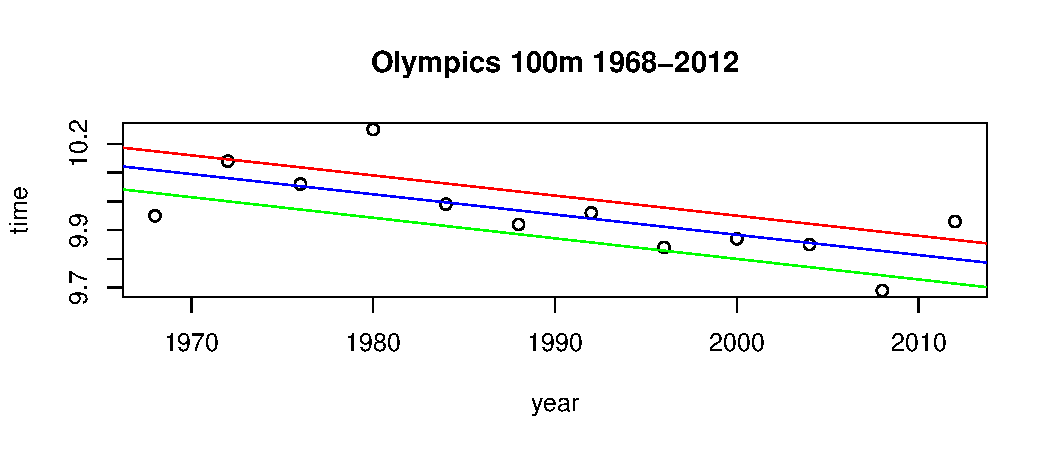
\includegraphics[width=\maxwidth]{figure/unnamed-chunk-45-1} 

\end{knitrout}
\end{itemize}
\end{frame}


\begin{frame}[fragile]{}
\begin{itemize}

\item 
For each candidate line $f(x)= a+bx$ for all $a$ and $b$, we focus on the resultant set of residuals: $res = e(a,b) = y-(a+bx)$. 

\vspace{.5cm}
This is the gaps between the line and the actual points.
For example, in the plot below the green residual is -0.1581 and the purple residual is 0.22603.
\end{itemize}

\begin{knitrout}
\definecolor{shadecolor}{rgb}{0.969, 0.969, 0.969}\color{fgcolor}
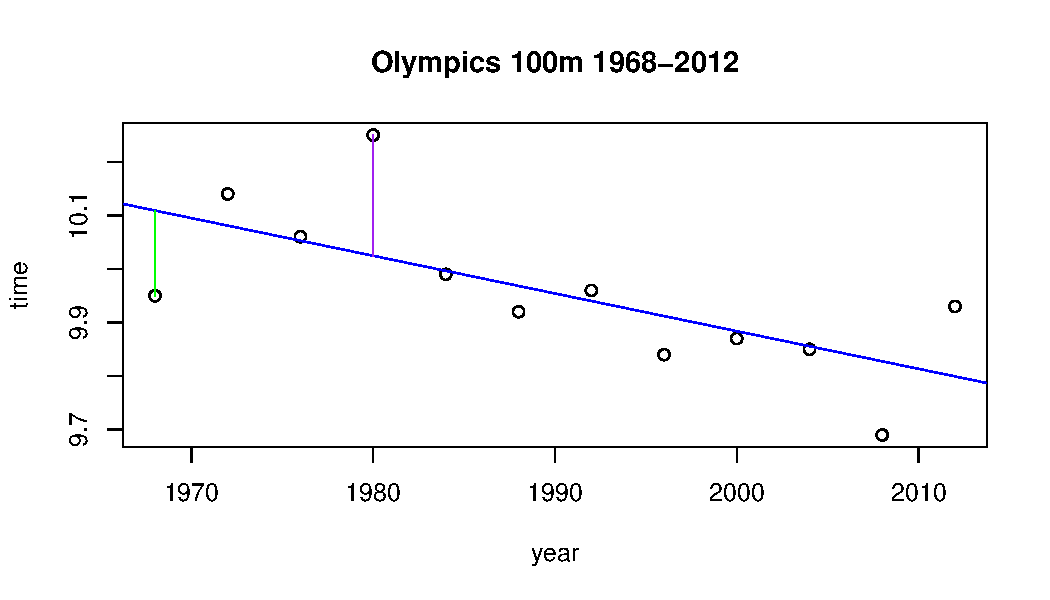
\includegraphics[width=\maxwidth]{figure/unnamed-chunk-46-1} 

\end{knitrout}
\end{frame}

\begin{frame}[fragile]{}

\begin{itemize}
\item   
We consider the `best’ line, to have the smallest residuals, determined by their sum of squared residuals 
\[ S(a,b)= \sum_{i=1}^{n} e(a,b)^2 = \sum_{i=1}^{n} (y - (a+bx))^2 \]

\item   
We minimise $S(a,b)$  by solving  $\frac{ \partial}{\partial a} = 0$ and 
$\frac{ \partial}{\partial b} = 0$. This gives 
 \[ \sum_{i=1}^{n} y_{i} - na - b \sum_{i=1}^{n} x_{i} = 0 \]
and
\[\sum_{i=1}^{n} x_{i} y_{i}  -  a \sum_{i=1}^{n} x_{i}   - b \sum_{i=1}^{n} x_{i}^2 = 0 \].

\end{itemize}
\end{frame}


\begin{frame}[fragile]{}

\begin{itemize}
\item
As long as the  $x_i$ are not all equal, there is a unique solution for the intercept and the slope,

\[  \boxed{ a = \bar{y} - b \bar{x}   } \]
and
\[ \boxed{ b = \frac { S_{xy} }{ S_{xx}} } \]
\end{itemize}




where    
\[ S_{xx} = \sum_{i=1}^{n} x_{i}^2 - \frac{1}{n} (\sum_{i=1}^{n} x_{i})^2 = (n-1) s_{x}^2 \]
\[ S_{yy} = \sum_{i=1}^{n} y_{i}^2 - \frac{1}{n} (\sum_{i=1}^{n} y_{i})^2 = (n-1) s_{y}^2 \]
\[ S_{xy} = \sum_{i=1}^{n} x_{i} y_{i} - \frac{1}{n} (\sum_{i=1}^{n} x_{i}) (\sum_{i=1}^{n} y_{i})  \]
and $s_{x}^2$ and $s_{y}^2$ are the variance of $\{ x \}$ and $\{ y \}$ respectively.

\end{frame}

\begin{frame}[fragile]{}

Note: The natural numerical summaries for bivariate data are:
$\bar{x}, \bar{y}, s_{x}, s_{y}$, so the LSL is a combination of these summaries: $\hat{y} = a+bx$.

\vspace{.5cm}
\begin{knitrout}
\definecolor{shadecolor}{rgb}{0.969, 0.969, 0.969}\color{fgcolor}\begin{kframe}
\begin{alltt}
\hlstd{model} \hlkwb{=} \hlkwd{lm}\hlstd{(time}\hlopt{~}\hlstd{year)}
\hlstd{model}\hlopt{$}\hlstd{coeff}
\end{alltt}
\begin{verbatim}
##  (Intercept)         year 
## 23.957226107 -0.007036713
\end{verbatim}
\end{kframe}
\end{knitrout}
\end{frame}

\begin{frame}[fragile]{}
\begin{knitrout}
\definecolor{shadecolor}{rgb}{0.969, 0.969, 0.969}\color{fgcolor}\begin{kframe}
\begin{alltt}
\hlkwd{plot}\hlstd{(year,time,} \hlkwc{xlab}\hlstd{=}\hlstr{"year"}\hlstd{,} \hlkwc{ylab}\hlstd{=}\hlstr{"time"}\hlstd{,}
     \hlkwc{main}\hlstd{=}\hlstr{"Olympics 100m 1968-2012"}\hlstd{)}
\hlkwd{abline}\hlstd{(model}\hlopt{$}\hlstd{coeff,} \hlkwc{col}\hlstd{=}\hlstr{"blue"}\hlstd{)}
\end{alltt}
\end{kframe}
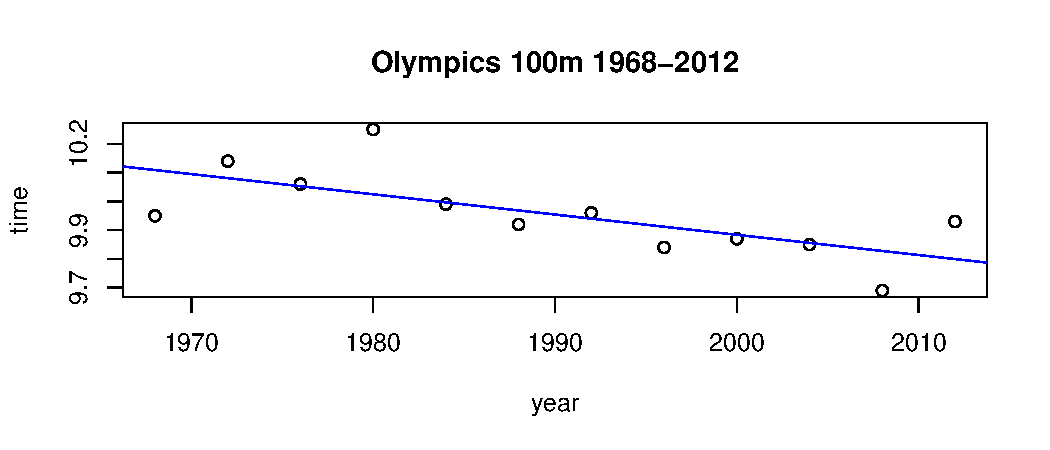
\includegraphics[width=\maxwidth]{figure/unnamed-chunk-48-1} 

\end{knitrout}
\end{frame}


\subsection[]{Step3: Construct a residual plot}
\begin{frame}[fragile]{Step3: Construct a residual plot}
A residual plot is a scatter plot of the residuals $res = e = y-(a+bx)$ vs $x$.

\vspace{.5cm}
It is a 2nd diagnostic: "Does the plot look random, or is there any pattern?"
\begin{itemize}
\item
  If the plot is random: then the LSL fit is good.
\item
	If the plot shows a relationship between $e$ and $x$, then the LSL is not adequate and we need to consider a more complex function or a transformation (eg $y=x^2$ or $y=log(x)$).
\end{itemize}
\end{frame} 
  
\begin{frame}[fragile]{}  
\begin{knitrout}
\definecolor{shadecolor}{rgb}{0.969, 0.969, 0.969}\color{fgcolor}\begin{kframe}
\begin{alltt}
\hlstd{residuals}\hlkwb{=}\hlstd{model}\hlopt{$}\hlstd{res}
\hlkwd{plot}\hlstd{(year,residuals,}\hlkwc{main}\hlstd{=}\hlstr{"Residual Plot"}\hlstd{)}
\hlkwd{abline}\hlstd{(}\hlkwc{h}\hlstd{=}\hlnum{0}\hlstd{,}\hlkwc{col}\hlstd{=}\hlstr{"red"}\hlstd{)}
\end{alltt}
\end{kframe}
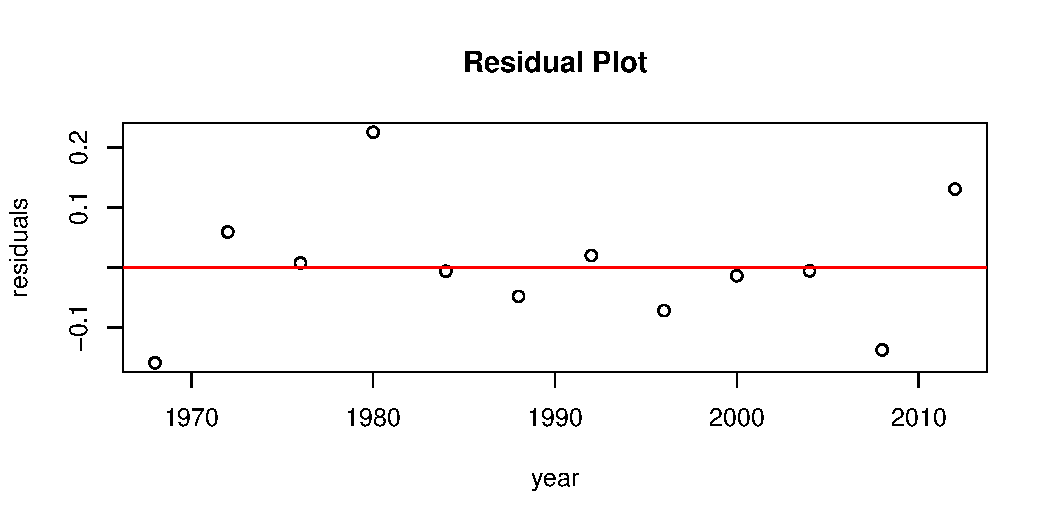
\includegraphics[width=\maxwidth]{figure/unnamed-chunk-49-1} 

\end{knitrout}
\end{frame}


\subsection[]{Step4: Calculate the correlation coefficient and the coefficient of determination}
\begin{frame}[fragile]{Step4: Calculate the correlation coefficient and the coefficient of determination}

We have calculated the ‘best’ line, but is it a good line? How strong is the linear relationship between $Y$ and $X$?

\vspace{.5cm}
A fit is considered good when the set of data points is close to the LSL, so that the residuals are small. So we consider the relationship between $s_{res}^2$ (the variance of the residuals) and $s_{y}^2$   (the variance of $y$).
\end{frame} 

\begin{frame}[fragile]{Pearson's correlation coefficient}
The correlation coefficient is
\[ \boxed{ r =  \frac{ S_{xy} }{\sqrt{ S_{xx} S_{yy}} } } \]

Properties:
\begin{itemize}
\item
$r$ is symmetric in $x$ and $y$.

\item $-1 \leq r \leq 1$ \\
$r$ is a numerical summary which indicates the strength of the linear assocation between $y$ and $x$.
\end{itemize}
\end{frame} 

\begin{frame}[fragile]{}
\begin{itemize}
\item  $r=\pm 1$ \\
This corresponds to a perfect linear correlation, with all the data points lying on the LSL.

\begin{knitrout}
\definecolor{shadecolor}{rgb}{0.969, 0.969, 0.969}\color{fgcolor}
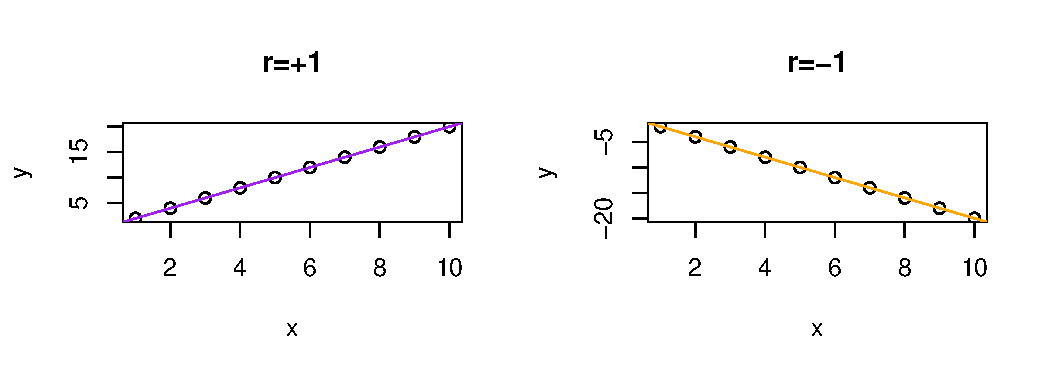
\includegraphics[width=\maxwidth]{figure/unnamed-chunk-50-1} 

\end{knitrout}
\end{itemize}
\end{frame} 

\begin{frame}[fragile]{}
\begin{itemize}
\item $r=0 $ \\
This indicates no linear correlation, for example a line with zero slope, or a random scatter, or a non linear relationship.
\end{itemize}
\begin{knitrout}
\definecolor{shadecolor}{rgb}{0.969, 0.969, 0.969}\color{fgcolor}
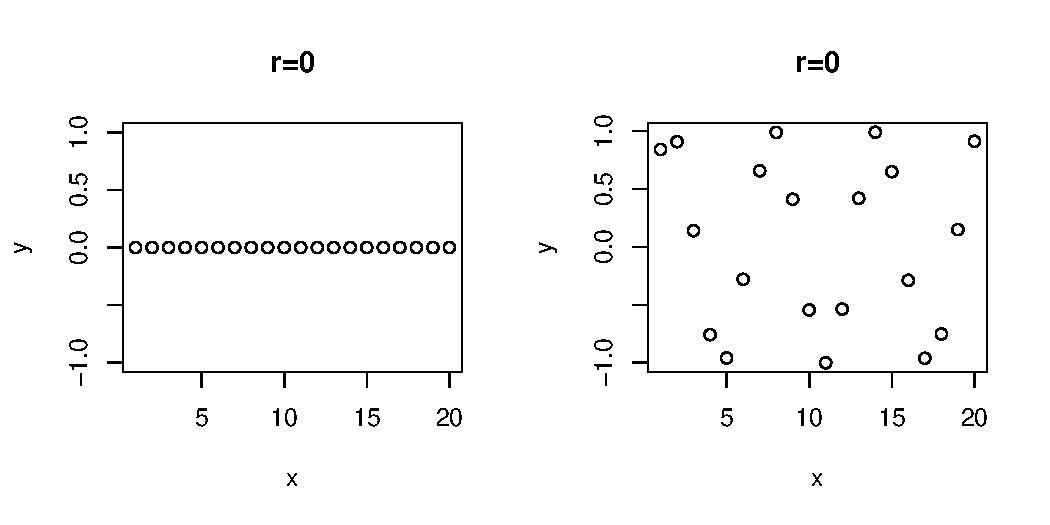
\includegraphics[width=\maxwidth]{figure/unnamed-chunk-51-1} 

\end{knitrout}
\end{frame} 

\begin{frame}[fragile]{Examples of Correlation Coefficients}
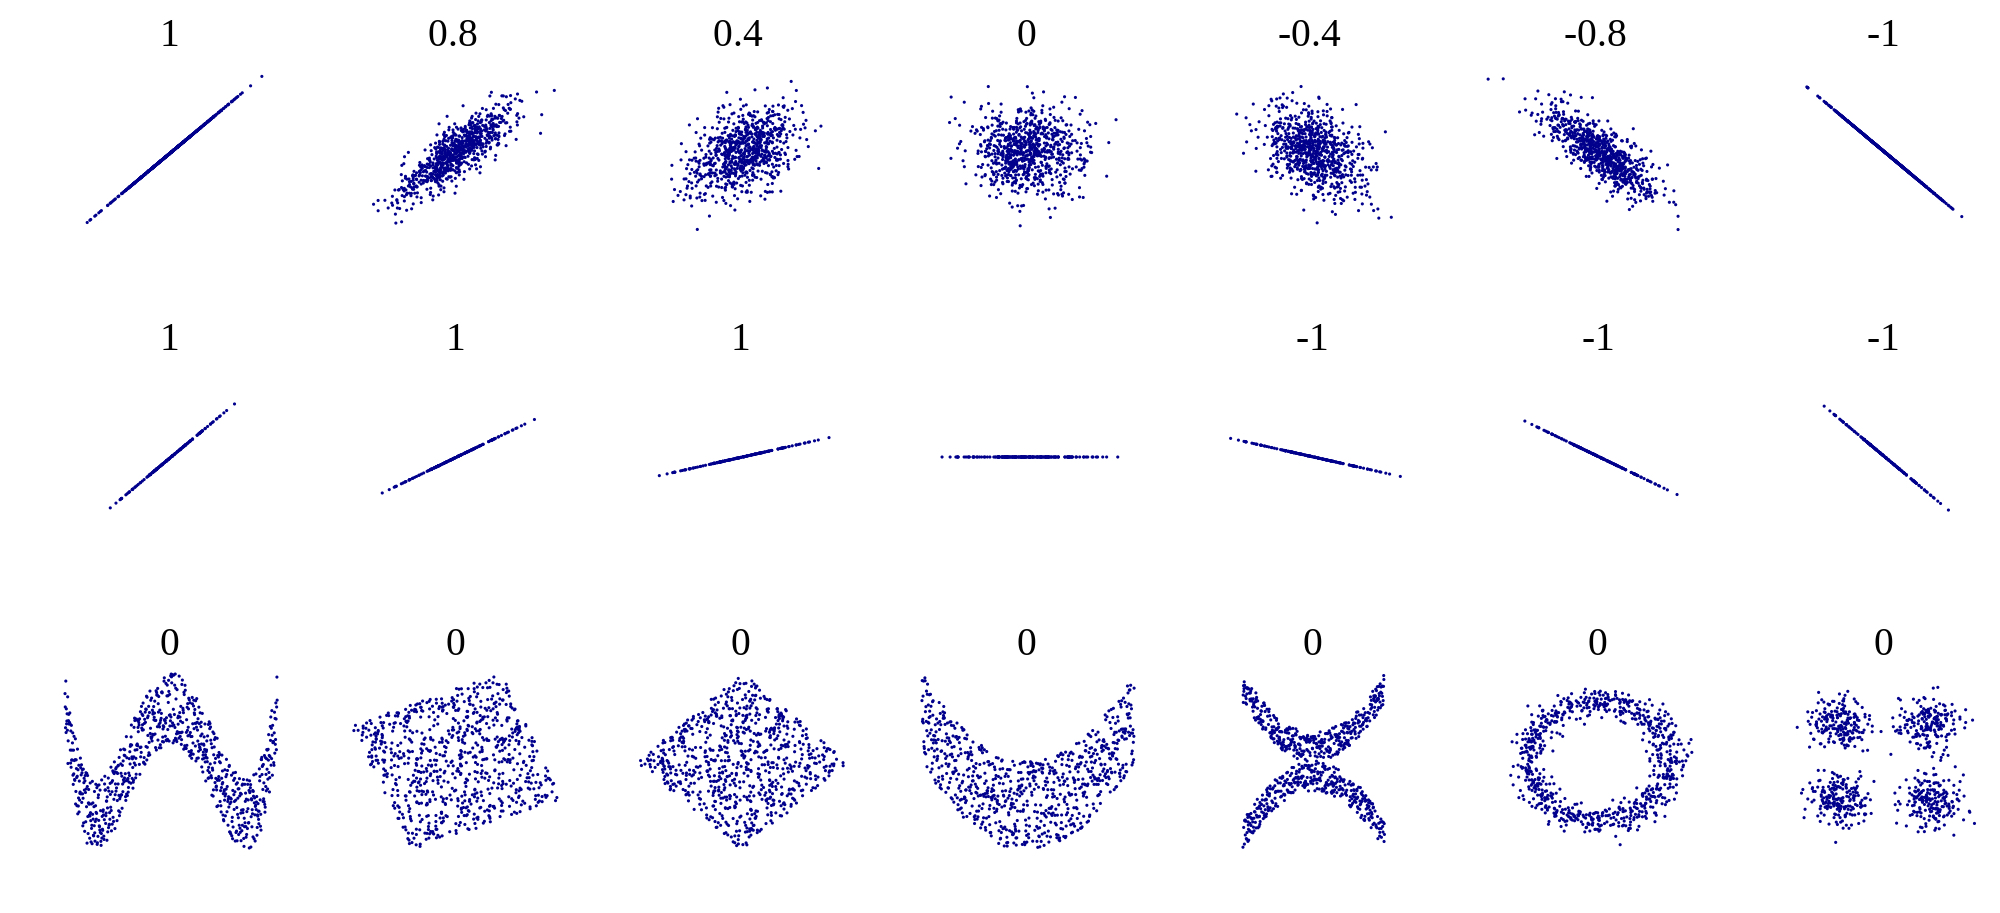
\includegraphics[height=5cm]{../images/CorrelationChart.jpg}

\href{https://en.wikipedia.org/wiki/Pearson_product-moment_correlation_coefficient}{\beamergotobutton{Link}}
\end{frame} 

\begin{frame}[fragile]{Relationship between Correlation Coefficient and Slope}
There is an interesting relationship between $r$ and $b$
\[ b =  \frac{ S_{xy} }{ S_{xx}  }
= \frac{ S_{xy} }{\sqrt{ S_{xx} S_{yy}} }   \frac{ \sqrt{ S_{yy} } }{ \sqrt{ S_{xx} } }
= r \frac{ \sqrt{ S_{yy}/(n-1)} }{ \sqrt{ S_{xx}/(n-1) }  }
= r \frac{ s_{y}}{s_{x}} \]

Hence:
\begin{itemize}
\item 
The sign of $r$ reflects the trend (slope) of the data.
\item
$r$ is unaffected by a change of scale or origin.
\end{itemize}
\end{frame} 

\begin{frame}[fragile]{The coefficient of determination}
The coefficient of determination is the proportion of variability of $y$ explained by $x$ for a model, or in our context, the proportion of variability explained by the linear regression. 

\[ \boxed{  r^2 = \frac{s_{y}^2 - s_{res}^2}{s_{y}^2} = \frac{S_{xy}^2}{S_{xx} S_{yy}}  }\]

Properties:
\begin{itemize}
\item $0 \leq r^2 \leq 1$ \\
%$r^2$ is a numerical summary: we say that $(1-r^2)100 \%$ of the variability of $y$ is explained by $x$.

\item  $r^2=1$ \\
This arises when $res_i=0 \;\; \forall i$ and $s_{res}^2=0$, ie all of the variability of the model is associated with the linear regression.
All points lie on the LSL.
\end{itemize}
\end{frame} 



\begin{frame}[fragile]{}

\begin{itemize}
\item  $r^2 \approx 1$ \\
This arises when $res_i=0$ is small compared to $s_{y}^2$, ie most of the variability of the model is associated with the linear regression.

\item $r^2=0$ \\
This arises when $s_{res}^2=s_{y}^2$, ie none the variability of the model is associated with the linear regression. 

\item $r^2 \approx 0$ \\
This arises when $s_{res}^2 \approx s_{y}^2$, ie almost none the variability of the model is associated with the linear regression. 

\item Note that $r^2$ can be small and still indicate that the model is correct (ie a model where there is naturally low association between $X$ and $Y$).

\end{itemize}
\end{frame} 

\begin{frame}[fragile]{}  
\begin{knitrout}
\definecolor{shadecolor}{rgb}{0.969, 0.969, 0.969}\color{fgcolor}\begin{kframe}
\begin{alltt}
\hlkwd{cor}\hlstd{(year,time)}
\end{alltt}
\begin{verbatim}
## [1] -0.6912573
\end{verbatim}
\begin{alltt}
\hlkwd{cor}\hlstd{(year,time)}\hlopt{^}\hlnum{2}
\end{alltt}
\begin{verbatim}
## [1] 0.4778366
\end{verbatim}
\end{kframe}
\end{knitrout}

Hence, the linear associotion between year and time for the Olympics 100m sprint is  -0.7 (fairly high). 48\% of the variation in times is explained by the variation in years.



\end{frame}



\subsection{Avoiding mistakes in Regression}
\begin{frame}[fragile]{Avoiding mistakes in Regression}

\begin{itemize}
\item Correlation does not imply causation \\
A high value of $r$ does not necessarily imply a causal relationship between $X$ and $Y$.  For example, December temperature and consumer spending).

\vspace{.5cm}
\item Causation does not imply (linear) correlation \\

\begin{knitrout}
\definecolor{shadecolor}{rgb}{0.969, 0.969, 0.969}\color{fgcolor}
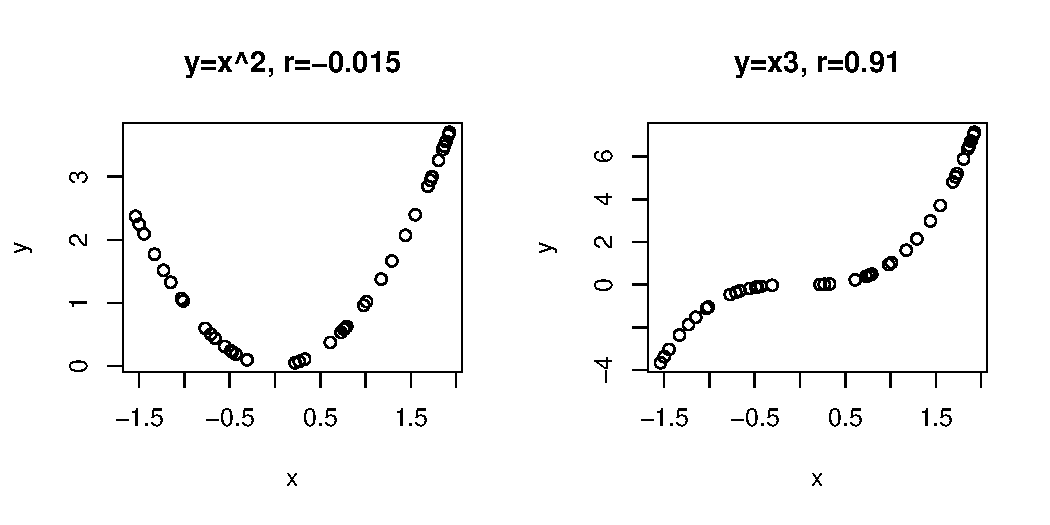
\includegraphics[width=\maxwidth]{figure/unnamed-chunk-53-1} 

\end{knitrout}
\end{itemize}
\end{frame} 


\begin{frame}[fragile]{Avoiding mistakes in Regression}
\begin{itemize}
\item The same value of $r$ can correspond to very different models.  \\

\vspace{.5cm}
The following data sets, called `Ansombe's Quartet' were constructed by Francis Anscombe in 1973. They all have $\bar{x}= 9$, $s_{x}^2=11$, $\bar{y} = 7.5$, $s_{y}^2 = 4.127$, $r=0.816$ and linear regression line $y=3+0.5x$. But look how different they look!
\end{itemize}

\href{https://en.wikipedia.org/wiki/Anscombes_quartet}{\beamergotobutton{Anscombes Quartet}}

\href{http://data.heapanalytics.com/anscombes-quartet-and-why-summary-statistics-dont-tell-the-whole-story}{\beamergotobutton{Law Grad salaries}}  %Why not work?
\end{frame} 


\begin{frame}[fragile]{}

\begin{knitrout}
\definecolor{shadecolor}{rgb}{0.969, 0.969, 0.969}\color{fgcolor}
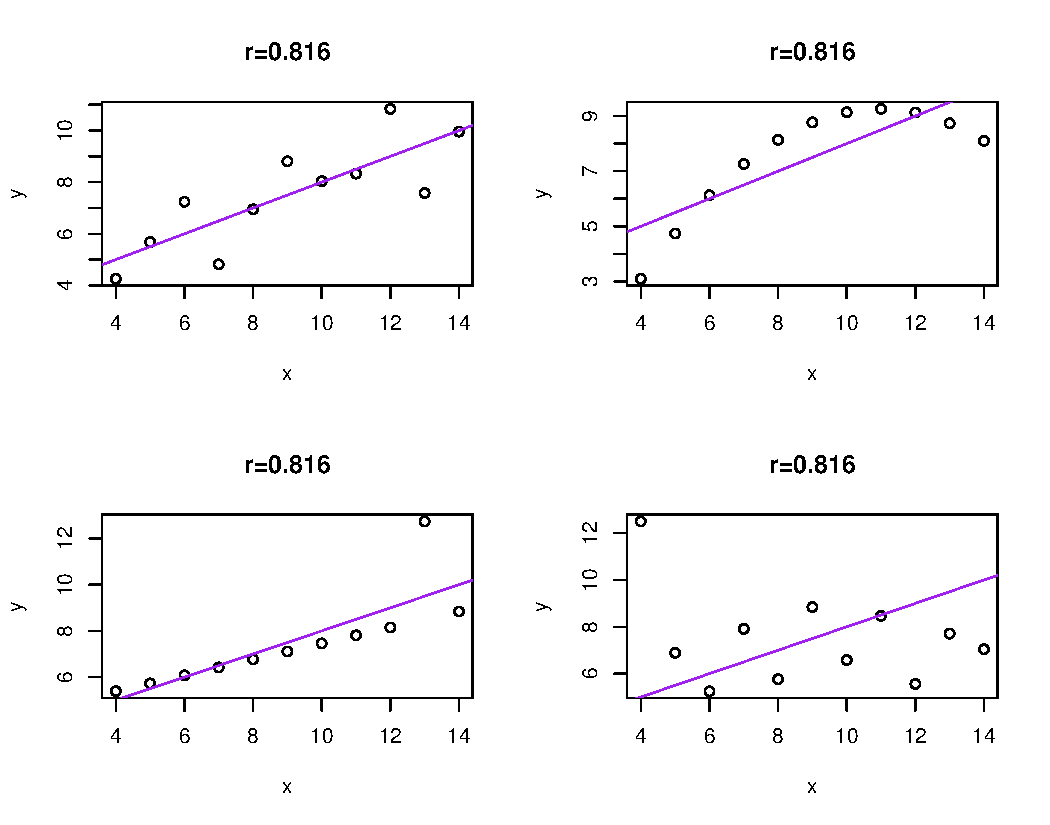
\includegraphics[width=\maxwidth]{figure/unnamed-chunk-54-1} 

\end{knitrout}
\end{frame} 


\begin{frame}[fragile]{}

\begin{itemize}
\item Even one outlier can distort the model.  \\

It's vital to draw a scatter plot before considering $r$, because of the high influence of outliers.

\begin{knitrout}
\definecolor{shadecolor}{rgb}{0.969, 0.969, 0.969}\color{fgcolor}
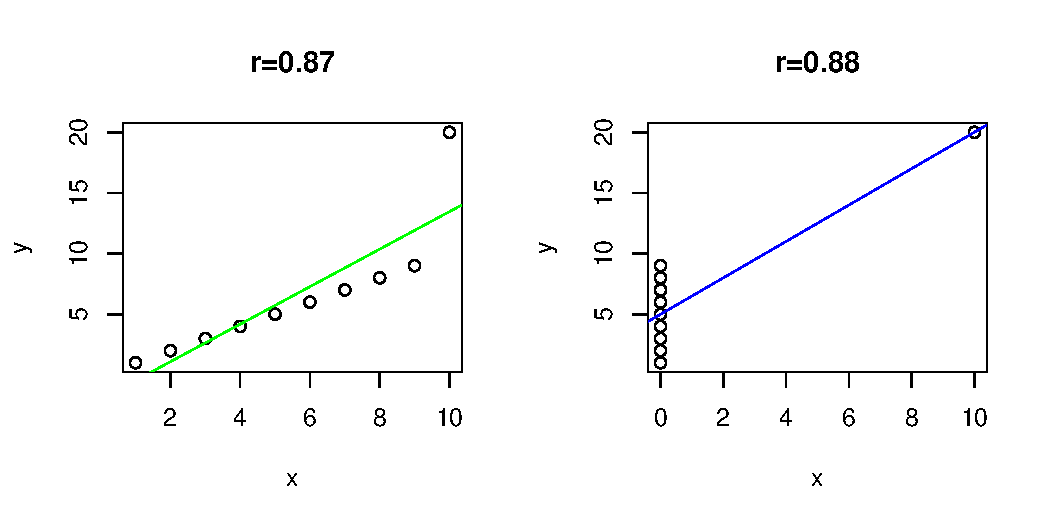
\includegraphics[width=\maxwidth]{figure/unnamed-chunk-55-1} 

\end{knitrout}
\end{itemize}
\end{frame} 


%%%% PART2 %%%%
\section[Part2]{PART2: PROBABILITY AND DISTRIBUTION THEORY (PDT)}
\subsection[]{Overview of Probability and Distribution Theory (PDT)}
\begin{frame}{Overview of Probability and Distribution Theory (PDT)}
``How does the population give rise to the data?" \\

\vspace{.5cm}
Probability and Distribution Theory (PDT) studies probability and distributions in order to model the population that gives rise to the sample.

\begin{center}
\begin{tikzpicture}[very thick, level distance = 2cm,
                    population/.style={rectangle,draw,fill=blue!20, draw},
                    sample/.style={rectangle,draw, rounded corners=.8ex},
                    %%every node/.style = {shape=rectangle, rounded corners,
                    %% draw, align=center,
                    %% top color=white, bottom color=blue!20}
                    ]]

\node[population, minimum height = 1.5cm, minimum width = 6cm] { Population  }
child { node[sample] {Sample}   };
\end{tikzpicture}
\end{center}
\end{frame}





%%%% TOPIC4 %%%%
\section[4]{Topic4: Probability, Random Variables and Distributions}

\subsection[]{Example: Coin Tossing during WWII}
\begin{frame}{Example: Coin Tossing during WWII}

John Edmund Kerrick (1903–1985) was a mathematician noted for a series of experiments in probability which he conducted while interned in Nazi-occupied Denmark (Viborg, Midtjylland) in the 1940s.  

\vspace{.5cm}
Kerrich had travelled from South Africa to visit his in-laws in Copenhagen, and arrived just 2 days after Denmark was invaded by Nazi Germany!

\begin{center}
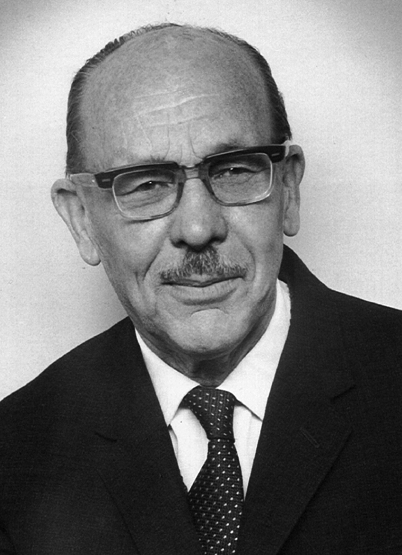
\includegraphics[height=4cm]{../images/KerrichBig.jpg}
\end{center}
\end{frame}

\begin{frame}{}

Fortunately Kerrich was imprisoned in a camp in Jutland run by the Danish Government in a `truly admirable way'. \\

\begin{center}
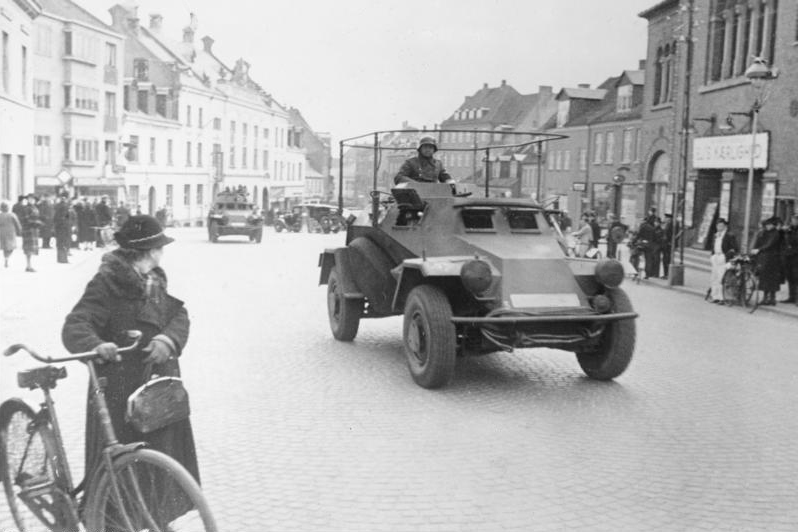
\includegraphics[height=5cm]{../images/Jutland.jpg}
\end{center}
\end{frame}

\begin{frame}{}

%'When Denmark was overrun by the Germans various British subjects were caught, Mr
%Kerrich among them. He was interned in a camp under Danish control
%and spent part of his enforced leisure in coin-tossing experiments' (Nature, 1946)

With a fellow internee Eric Christensen, Kerrich set up a sequence of experiments demonstrating the empirical validity of a number of fundamental laws of probability.

\begin{itemize}
\item They tossed a coin 10,000 times and counted the number of heads. \\
\item They made 5000 draws from a container with 4  ping pong balls (2x2 different brands), 'at the rate of 400 an hour, with - need it be stated - periods of rest between successive hours.'
\item They investigated tosses of a `biased coin', made from a wooden disk partly coated in lead.
\end{itemize}

In 1946 Kerrich published his finding in a monograph, {\it An
Experimental Introduction to the Theory of Probability}. 
\href{http://www.maths.usyd.edu.au/u/UG/JM/MATH1005/r/StatsData/Kerrich1950.pdf}{\beamergotobutton{Kerrich1950Paper}}

\vspace{.5cm}
{\bf How many heads do you think he counted? What is the probability of getting a head on a fair coin?}

\end{frame}

\subsection[]{Why study Probability?}
\begin{frame}{Why study Probability?}

Probability is often perceived as ‘scary’ because it conjures up impossible problems from School Maths Competitions! However ...

\begin{enumerate}
\item Probability is an essential part of every day life.  \\
 ``The most important questions of life ... are indeed for the most part only problems of probability."
 
 {\tiny (Laplace, {\it Théorie Analytique des Probabilitiés}, 1814)}
\href{http://bayes.wustl.edu/Manual/laplace_A_philosophical_essay_on_probabilities.pdf}{\beamergotobutton{Laplace1}}

\item 
Probability Theory makes many school problems easy. \\
``The theory of probabilities is basically just common sense reduced to calculus." 

{\tiny (Laplace, {\it Essai philosophique sur les probabilités},  1814)}
\href{http://archive.org/details/essaiphilosophiq00lapluoft}{\beamergotobutton{Laplace2}}

\item Probability (or the $p$-value) is crucial for decision making in Hypothesis Testing, which is essential to scientific research (Part 3).
\end{enumerate}
\end{frame}


\subsection[]{What is Probability?}
\begin{frame}{What is Probability?}

\begin{block}{Definition (Probability)}
The probability of an event is a measure of the likelihood of that event occurring. 
\end{block}

%Many systems are so complex that we rarely know the initial conditions accurately and so cannot predict outcomes (Newtonian physics).  Hence we adopt a stochastic viewpoint:  we identify the set of possible outcomes, and ascribe to each outcome (or set of outcomes) a probability $p  \in [0,1]$.

\vspace{.5cm}
Probability Theory is a set of mathematical tools which dates back centuries to casino type games. A more formal theory was developed in the 1930s by the Russian mathematician A. N. Kolmogorov.
\href{http://www.youtube.com/watch?v=2y3PH4SqmlA}{\beamergotobutton{History Video}}
\hyperlink{Appendix1}{\beamergotobutton{Appendix}}
\end{frame}

\subsection[]{Three types of Probability}
\begin{frame}{Three types of Probability}

{\bf (1) Subjective probability: based on belief} \\
The probability of an event is based on the strength of one’s belief.

\vspace{.5cm}
\begin{block}{Tossing a Fair Coin}
If I toss a fair coin once, the probability of getting a head is … 
\end{block}
\end{frame}


\begin{frame}{}

We rely on subjective probability for everyday decisions. But it can be abused.

\vspace{.5cm}
On March 27 1977 a PanAm 747 jet and a KLM 747 jet collided on an airport
runway in the Canary Islands killing 583 people.  Both jets had been scheduled for the Las Palmas Airport, but were diverted to Los Rodeos Airport (now called Tenerife) after  a group of militants set off a small bomb at the airport’s flower shop earlier that day. 

\begin{center}
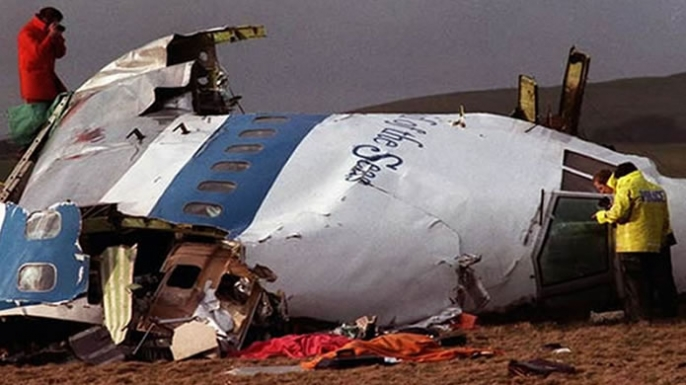
\includegraphics[height=3cm]{../images/Canary1.jpg}
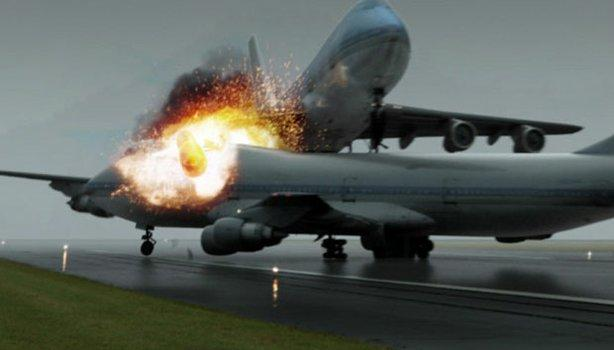
\includegraphics[height=3cm]{../images/Canary2Animation.jpg}
\end{center}
\end{frame}

\begin{frame}{}
The following statement was released: \\

\vspace{.5cm}
{\it NEW YORK, Mon: Mr. Webster Todd, Chairman
of the American National Transportation Safety Board
said today statistics showed that the chances of two
jumbo jets colliding on the ground were about 6 million
to one.} (AAP, quoted in West Australian, 1977)
\end{frame}


\begin{frame}{}
Australian statistician Terry Speed questioned the Chairman, with the following response: \\

\vspace{.5cm}
{\it Dear Professor Speed, \\
In response to your aerogram of April 5, 1977, the
Chairman’s statement concerning the chances of two
jumbo jets colliding (6 million to one) has no statistical
validity nor was it intended to be a rigorous or precise
probability statement. The statement was made to
emphasize the intuitive feeling that such an occurrence
indeed has a very remote but not impossible chance of
happening.
Thank you for your interest in this regard.}
\end{frame}



\begin{frame}{}

{\bf (2) Frequentist (or simulation) probability: based on data} \\
The probability of an event is the proportion of times that event would occur in a large number of repeated experiments (simulation).

\vspace{.5cm}
In some ways, subjective probability is an informal version of frequentist probability, using one's own history and experience (`personal data') as the basis.

\vspace{.5cm}
\begin{block}{Tossing a Fair Coin}
The probability of tossing a fair head =  $P(H)$ = The long run proportion of heads if we toss a fair coin a large number of times.
\end{block}
\end{frame}

\begin{frame}[fragile]{}

Famous Coin Tossers

\vspace{.5cm}
{\tiny \begin{tabular}{llll}
{\bf Person} & {\bf Number of Tosses} $n$ & {\bf Number of Heads} $x$ & $P(Head)$  \\  \hline
Count Buffon (1707-1788) 
\href{https://en.wikipedia.org/wiki/Georges-Louis_Leclerc,_Comte_de_Buffon}{\beamergotobutton{Buffon}}
& 4040 & 2048 & 0.507 \\ \hline
Karl Pearson (1857-1936) 
\href{https://en.wikipedia.org/wiki/Karl_Pearson}{\beamergotobutton{Pearson}}
& 24000 & 12012 & 0.5005 \\ \hline
John Kerrick (1903-1985 war camp) 
\href{https://en.wikipedia.org/wiki/John_Edmund_Kerrich}{\beamergotobutton{Kerrick}}
& 10000 & 5067 & 0.5067 \\ \hline
Perci Diaconis (1945-present) 
\href{http://statweb.stanford.edu/~susan/papers/headswithJ.pdf}{\beamergotobutton{Diaconis}}
& machine & & 0.51 \\ \hline
\end{tabular}}

\vspace{.5cm}
\begin{center}
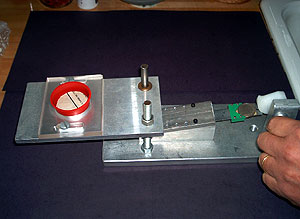
\includegraphics[height=4cm]{../images/CoinTosser.jpg}
\end{center}
\end{frame}

\begin{frame}[fragile]{}

In R Simulations

\begin{knitrout}
\definecolor{shadecolor}{rgb}{0.969, 0.969, 0.969}\color{fgcolor}\begin{kframe}
\begin{alltt}
\hlkwd{table}\hlstd{(}\hlkwd{sample}\hlstd{(}\hlkwd{c}\hlstd{(}\hlstr{"H"}\hlstd{,}\hlstr{"T"}\hlstd{),}\hlnum{4040}\hlstd{,}\hlkwc{replace}\hlstd{=T))}\hlopt{/}\hlnum{4040}
\end{alltt}
\begin{verbatim}
## 
##         H         T 
## 0.4970297 0.5029703
\end{verbatim}
\begin{alltt}
\hlkwd{table}\hlstd{(}\hlkwd{sample}\hlstd{(}\hlkwd{c}\hlstd{(}\hlstr{"H"}\hlstd{,}\hlstr{"T"}\hlstd{),}\hlnum{24000}\hlstd{,T))}\hlopt{/}\hlnum{24000}
\end{alltt}
\begin{verbatim}
## 
##      H      T 
## 0.4985 0.5015
\end{verbatim}
\begin{alltt}
\hlkwd{table}\hlstd{(}\hlkwd{sample}\hlstd{(}\hlkwd{c}\hlstd{(}\hlstr{"H"}\hlstd{,}\hlstr{"T"}\hlstd{),}\hlnum{10000}\hlstd{,T))}\hlopt{/}\hlnum{10000}
\end{alltt}
\begin{verbatim}
## 
##      H      T 
## 0.4954 0.5046
\end{verbatim}
\end{kframe}
\end{knitrout}

\end{frame}

\begin{frame}{}
Kerrich's Tosses: Proportion of Heads
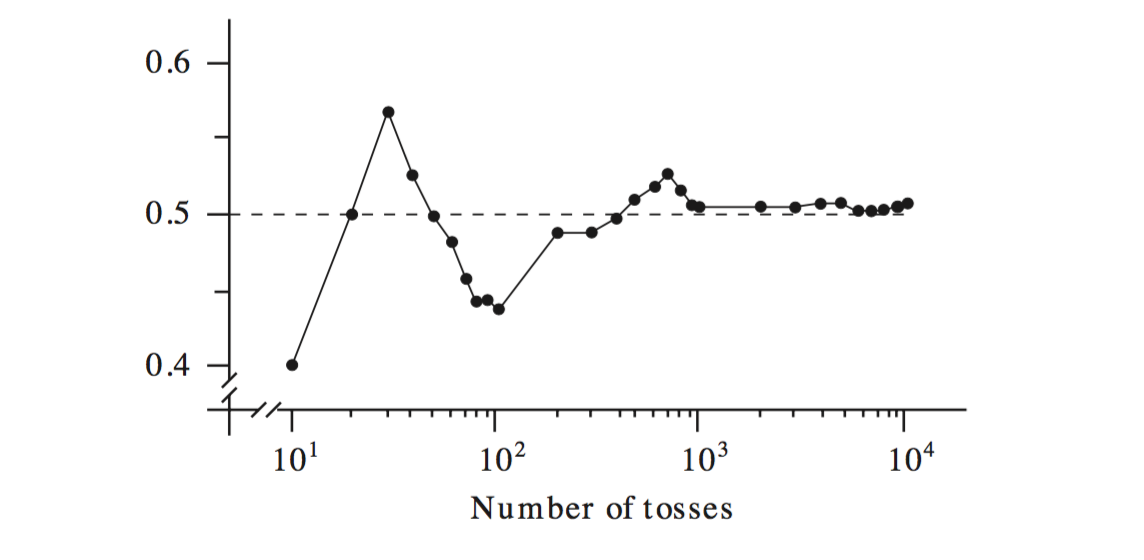
\includegraphics[height=6cm]{../images/KerrichTosses.jpg}

This illustrates the `Law of Averages' or `Law of Large Numbers': the proportion of heads becomes more stable as the length of the simulation increases and approaches a fixed number called the `relative frequency'.

\end{frame}


\begin{frame}{}

{\bf (3) Theoretical (or classical) probability: based on model} \\
The probability of an event is based on a model of the context. 

\vspace{.5cm}
Two models for Coin Tossing: 

\vspace{.5cm}
(1) Physics model: the side that the coin lands on is determined by a number of complicated factors such as which way up it started, the degree of spin, the speed and angle with which it left the thumb and how far it has to fall.
\href{https://www.youtube.com/watch?v=AYnJv68T3MM}{\beamergotobutton{PercisDiaconisVideo1}} 
\href{https://www.youtube.com/watch?v=Obg7JPd6cmw}{\beamergotobutton{PercisDiaconisVideo2}}

\begin{center}
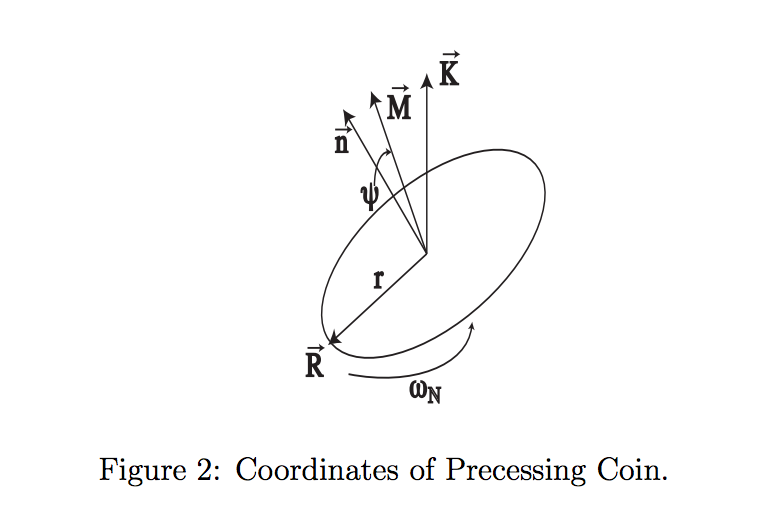
\includegraphics[height=3cm]{../images/CoinPhysics.jpg}
\end{center}

\end{frame}

\begin{frame}{}

(2) Standard model: Tossing a fair coin results in a head and a tail half the time, in an unpredictable order (random). 

\vspace{.5cm}
\begin{block}{Tossing a Fair Coin}
Given a coin toss has 2 outcomes, the probability of tossing a fair head =  $\frac{1}{2}$.
\end{block}

\vspace{.5cm}
This is the model used for decisions in sport (eg which team starts with the ball in AFL, or which team bats or bowls first in cricket).

\begin{center}
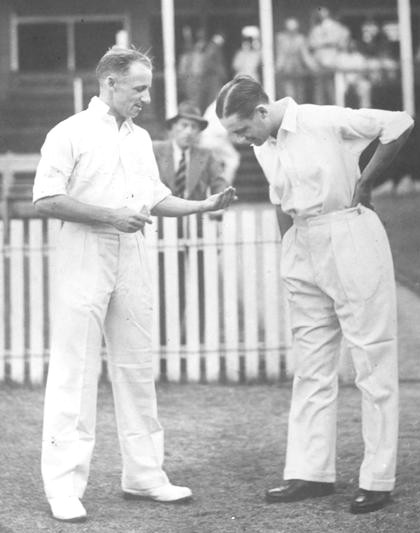
\includegraphics[height=3cm]{../images/BradmanAllenToss.jpg}
\end{center}

\vspace{.5cm}
{\tiny Note: In later Stats courses, you will also learn about Bayesian Probability.}

\end{frame}


\begin{frame}[fragile]{}
\begin{alertblock}{Extension}
Suppose you toss a fair coin 1000 times:  when it lands heads
you receive \$1, and when it lands tails you pay me \$1.
What is your expected profit or loss?
\end{alertblock}

Using Simulation:
\begin{knitrout}
\definecolor{shadecolor}{rgb}{0.969, 0.969, 0.969}\color{fgcolor}\begin{kframe}
\begin{alltt}
\hlkwd{set.seed}\hlstd{(}\hlnum{1}\hlstd{)}
\hlstd{CoinTosses} \hlkwb{<-} \hlkwd{sample}\hlstd{(}\hlkwd{c}\hlstd{(}\hlopt{-}\hlnum{1}\hlstd{,}\hlnum{1}\hlstd{),} \hlnum{1000}\hlstd{,} \hlkwc{replace} \hlstd{=} \hlnum{TRUE}\hlstd{)}
\hlkwd{plot}\hlstd{(}\hlkwd{cumsum}\hlstd{(CoinTosses),}\hlkwc{xlab}\hlstd{=}\hlstr{"Tosses"}\hlstd{,} \hlkwc{ylab}\hlstd{=}\hlstr{"P/L"}\hlstd{,} \hlkwc{type}\hlstd{=}\hlstr{"l"}\hlstd{)}
\end{alltt}
\end{kframe}
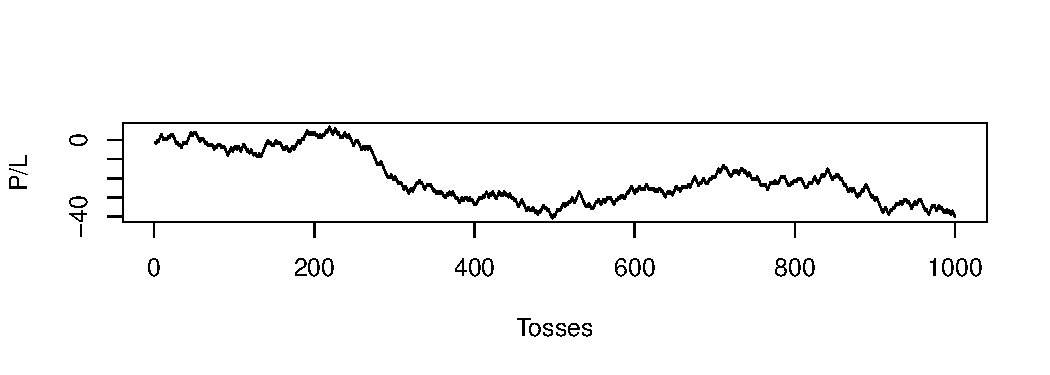
\includegraphics[width=\maxwidth]{figure/unnamed-chunk-58-1} 

\end{knitrout}
\end{frame}


\begin{frame}{}
We could run this simulation 10000 times, resulting in:

\begin{knitrout}
\definecolor{shadecolor}{rgb}{0.969, 0.969, 0.969}\color{fgcolor}
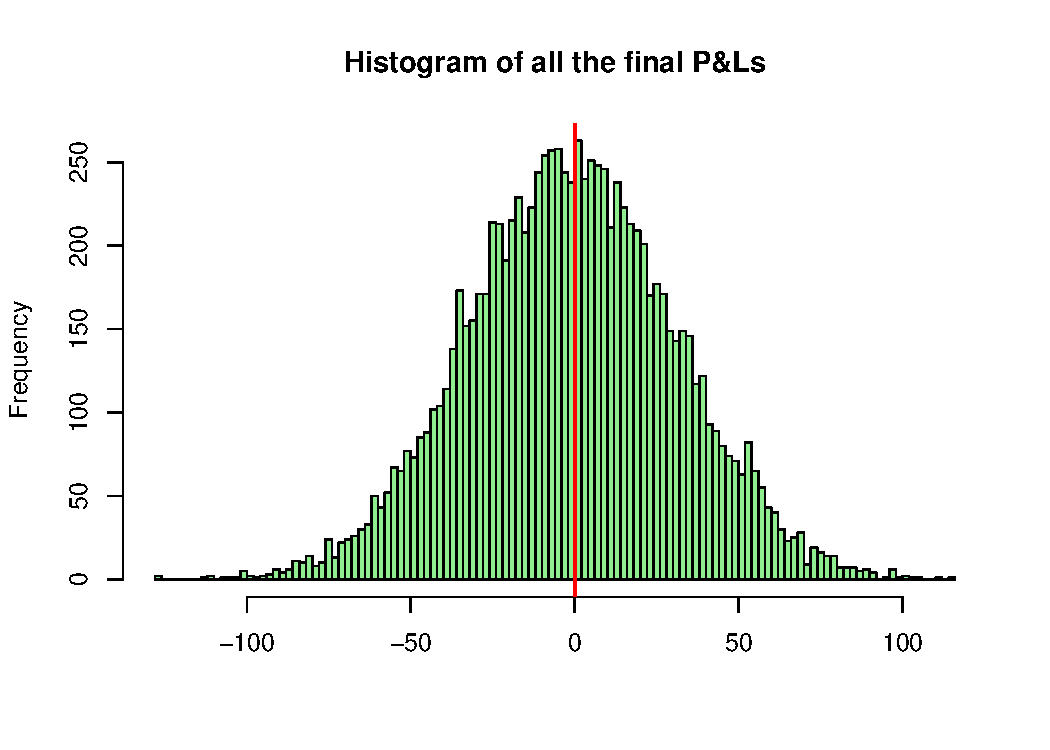
\includegraphics[width=\maxwidth]{figure/unnamed-chunk-59-1} 

\end{knitrout}

In Topic 5, we will see how to solve this theoretically.

\end{frame}


\subsection[]{Describing Simple Probability Models}

\begin{frame}[fragile]{Describing Simple Probability Models}
We can describe simple probability models using set notation and the Venn diagram.

\vspace{.5cm}
\begin{tabular}{lll}
Symbol & Name & Meaning \\ \hline
$\Omega$ & Sample Space & Everything that can occur. \\
$A, B, \ldots$ & Events & A subset of the sample space. \\ $\emptyset$  & Empty Set & An event which cannot occur. \\
 $A^{'}$ or $A^c$ & Complement & Everything not in $A$. \\
$A \subset \Omega$  & Belongs to & Event A belongs to sample space $\Omega$. \\
\end{tabular}

\begin{center}
\begin{tikzpicture}
\draw (-3,-1.5) rectangle (3,1.5) node[below left]{$\Omega$}
 node[below right]{$A \subset \Omega$};
\fill[green] (0,0) circle (1cm);
\draw (0,0) circle (1cm) node {$A$};
\end{tikzpicture}
\end{center}

\end{frame}


\begin{frame}[fragile]{}

{\bf If $A$ and $B$ $\subset \Omega$:} 

\vspace{.5cm}
\begin{tabular}{lll}
Symbol & Name & Meaning \\ \hline
$A \cup B$ & Union & $A$ or $B$ or both occur. \\
$A \cap B$ & Intersection & Both $A$ and $B$ occur. \\
$A  \setminus B$ & Minus or Relative Complement & In $A$ but  not in $B$. \\
\end{tabular}

%% Picture of A Union B
\vspace{1cm}
\begin{center}
\begin{tikzpicture}
\draw (-2,-1.5) rectangle (3.5,1.5) node[below left]{$\Omega$}  node[below right]{$A \cup B $};
\fill[green] (0,0) circle (1cm);
\fill[green] (1.5,0) circle (1cm);
\draw (0,0) circle (1cm) node {$A$};
\draw (1.5,0) circle (1cm) node {$B$};
\end{tikzpicture}
\end{center}
\end{frame}

%% Picture of A Intersection B
\begin{frame}
\begin{center}
\begin{tikzpicture}
\draw (-2,-1.5) rectangle (3.5,1.5) node[below left]{$\Omega$} node[below right]{$A \cap B $};
\begin{scope} % start of clip scope
\clip (0,0) circle (1cm);   % keep only what is inside A
\fill[green] (1.5,0) circle (1cm);   % draw region B
\end{scope} % end of clip scope
\draw (0,0) circle (1cm) node[left] {$A$};
\draw (1.5,0) circle (1cm) node[right] {$B$};
\end{tikzpicture}
\end{center}

%% Picture of A Minus B
\begin{center}
\begin{tikzpicture}
\draw (-2,-1.5) rectangle (3.5,1.5) node[below left]{$\Omega$} node[below right]{$A \setminus B $};
\begin{scope}{even odd rule} % start of clip scope
\clip (1.5,0) circle (1cm) (-2,-1.5) rectangle (3.5,1.5);   % complement of B
\fill[green] (0,0) circle (1cm);   % draw region A
\end{scope} % end of clip scope
\draw (0,0) circle (1cm) node[left] {$A$};
\draw (1.5,0) circle (1cm) node[right] {$B$};
\end{tikzpicture}
\end{center}
\end{frame}



\begin{frame}[fragile]{}
\vspace{.5cm}
{\bf If $A_{1}, A_{2}, \ldots \subset \Omega$:} 

\vspace{.5cm}
\begin{tabular}{lll}
Symbol & Name & Meaning \\ \hline
$\cup A_{i=1}^{n}$ & Union & One or more of $A_{i}$ occur. \\
$\cap A_{i=1}^{n}$ & Intersection & All $A_{i}$ occur. \\
\end{tabular}
\end{frame}


\begin{frame}{Example}
\begin{alertblock}{Your Turn (Set Notation)}
Describe the grey and white regions in set notation.
% Grey = $A \cap B \cap C'$; White = $ A \cap B \cap C$
\begin{center}
\begin{tikzpicture}
\draw \setO node[below left]{$\Omega$};
\begin{scope}
\clip \setA;
\fill[gray] \setB;
\end{scope}
\begin{scope}
\clip \setA;
\clip \setB;
\fill[white] \setC;
\end{scope}
\draw \setA node[left] {$A$};
\draw \setB node[right] {$B$};
\draw \setC node {$C$};
\end{tikzpicture}
\end{center}
\end{alertblock}
\end{frame}


\begin{frame}{}
\begin{alertblock}{Your Turn (Sample Space)}
\begin{itemize}

\item A coin is tossed to start a cricket match. What is the probability of landing on its edge? \\

\item For the following scenarios, what is $\Omega$?

\begin{itemize} 
\item A coin is tossed until a head occurs. 
\item The 2016 Australian census question about Gender.
\item Measuring tomorrow's rainfall.
\end{itemize}
\end{itemize}

\end{alertblock}
\end{frame}


\subsection[]{Probability Results}
\begin{frame}[fragile]{Probability Results}

\begin{itemize}
\item 
Classical Probability \\
Where the sample space $\Omega$ consist of a finite, known number of equally likely outcomes (eg coins, dice, cards), 
the probability of an event $A \subset \Omega$ occurring is 

\[\boxed{ P(A) = \frac{\mbox{Number of ways $A$ can occur}}{\mbox{Total number of possible outcomes in } \Omega} }  \] 

\vspace{.5cm}
where \\
$P(A) = 0$ (impossible event)  \\
$P(A) = 1$ (certain event) \\
\end{itemize}
\end{frame}
 
\begin{frame}\frametitle{}  
\begin{itemize}
\item
Complement \\
The probability that an event $A$ does not occur is

\[ \boxed{ P(A') = 1 - P(A)  }\]

\vspace{.5cm}
\item Mutually Exclusive \\
2 events $A$ and $B$ are mutually exclusive if
\[ \boxed{ P(A \cap B) = 0 } \]

\vspace{.25cm}
%% Picture of Mutually Exclusive
\begin{center}
\begin{tikzpicture}
\draw (-2,-1.5) rectangle (6,1.5) node[below left]{$\Omega$}  node[below right]{};
\draw (0,0) circle (1cm) node {$A$};
\draw (3,0) circle (1cm) node {$B$};
\end{tikzpicture}
\end{center}
\end{itemize}

Note: This is not a 'rule' but a definition. We position it here, to see comparison with independence.
\end{frame} 


\begin{frame}[label=Setindependence]\frametitle{} 
\begin{itemize}
\item Independence \\
2 events $A$ and $B$ are independent (the result of one does not affect the result of the other) iff

\[ \boxed{ P(A \cap B) = P(A)P(B)  }\]

\vspace{.5cm}
%% Picture of Independent Events
\begin{center}
\begin{tikzpicture}
\draw (-2,-1.5) rectangle (3.5,1.5) node[below left]{$\Omega$} node[below right]{\tiny{$P(A)=0.2$, $P(B)=0.5$, $P(A \cap B) = 0.1$}};
\begin{scope} % start of clip scope
\clip (0,0) circle (1cm);   % keep only what is inside A
\fill[green] (1.5,0) circle (1cm);   % draw region B
\end{scope} % end of clip scope
\draw (0,0) circle (1cm) node[left] {$A$};
\draw (1.5,0) circle (1cm) node[right] {$B$};
\end{tikzpicture}
\end{center}
\end{itemize}
\end{frame}
 
\begin{frame}\frametitle{} 
\begin{itemize}

\item Union Rule \\
For events $A$ and $B \subset \Omega$, then 

\[ \boxed{ P(A \cup B) = P(A) + P(B) – P(A \cap B) } \]

\vspace{.5cm}
%% Picture of A Union B
\begin{center}
\begin{tikzpicture}
\draw (-2,-1.5) rectangle (3.5,1.5) node[below left]{$\Omega$}  node[below right]{};
\fill[green] (0,0) circle (1cm);
\fill[green] (1.5,0) circle (1cm);
\draw (0,0) circle (1cm) node {$A$};
\draw (1.5,0) circle (1cm) node {$B$};
\end{tikzpicture}
\end{center}
\end{itemize}
\end{frame}

\begin{frame}{}

For mutually exclusive events, this reduces to

\[ \boxed{ P(A \cup B) = P(A) + P(B) } \]

\vspace{.5cm}
%% Picture of A Union B
\begin{center}
\begin{tikzpicture}
\draw (-2,-1.5) rectangle (5,1.5) node[below left]{$\Omega$}  node[below right]{};
\fill[green] (0,0) circle (1cm);
\fill[green] (2.5,0) circle (1cm);
\draw (0,0) circle (1cm) node {$A$};
\draw (2.5,0) circle (1cm) node {$B$};
\end{tikzpicture}
\end{center}
\end{frame}
 
\begin{frame}\frametitle{} 
\begin{itemize}

\item Conditional Probability \\
For events $A$ and $B \subset \Omega$ where $P(B) \neq 0$, the conditional probability of $A$ given $B$ is

\[  \boxed{ P(A | B) = \frac{ P(A \cap B)}{P(B)} } \]

\vspace{.5cm}
This leads to a second definition of independence:

2 events $A$ and $B$ are independent iff

\[ \boxed{ P(A | B) = P(A)  }\]

\end{itemize}
\end{frame}

\begin{frame}\frametitle{} 
\begin{itemize}

\item Bayes Theorem

\[  \boxed{ P(A | B) = \frac{ P(B | A) P(A)}{P(B)} } \]

\href{https://en.wikipedia.org/wiki/Confusion_of_the_inverse}{\beamergotobutton{Bayes Theorem}}

\vspace{.5cm}
\item The Law of Total Probability
 
 \[ \boxed{  P(A) = \sum_{i}^{} P(A | B_{i}) P(B_{i}) } \]
 
 for any $i$ for which $P(B_{i}) \neq 0$.

\end{itemize}
\end{frame}

\subsection[]{Counting Short Cuts}
\begin{frame}[label=Factorials]{Counting Short Cuts}
\frametitle{} 

Computing classical probabilities amounts to careful counting, so we have the following short-cuts.

\vspace{.5cm}
\begin{block}{Multiplication Principle for $k$ stage problems}
If an experiment consists of $k$ stages where the $i$th stage has $n_{i}$ outcomes (for $i=1,2,\ldots k$), then the total number of outcomes is $n_{1} n_{2} \ldots n_{k}$.
\end{block}

\vspace{.5cm}
\begin{block}{Definition (Permutations, Factorials)}
Any $x$ distinct objects can be permuted (or rearranged) in $x! = x(x-1)(x-2) \ldots 3 2 1$ ways.
\end{block}
\end{frame}

\begin{frame}[label=BinomialCoefficients,fragile]
\frametitle{} 

\begin{block}{Definition (Combinations, Binomial Coefficients)}
The number of ways of choosing a group of $x$ objects from $n$ objects is 
\[ {n \choose x}  = \frac{n!}{x! (n-x)!} \]
where by definition $0! = 1$.
\end{block}

\begin{knitrout}
\definecolor{shadecolor}{rgb}{0.969, 0.969, 0.969}\color{fgcolor}\begin{kframe}
\begin{alltt}
\hlkwd{factorial}\hlstd{(}\hlnum{10}\hlstd{)}\hlopt{/}\hlstd{(}\hlkwd{factorial}\hlstd{(}\hlnum{8}\hlstd{)}\hlopt{*}\hlkwd{factorial}\hlstd{(}\hlnum{2}\hlstd{))}
\end{alltt}
\begin{verbatim}
## [1] 45
\end{verbatim}
\begin{alltt}
\hlkwd{choose}\hlstd{(}\hlnum{10}\hlstd{,}\hlnum{2}\hlstd{)}
\end{alltt}
\begin{verbatim}
## [1] 45
\end{verbatim}
\end{kframe}
\end{knitrout}
\end{frame}
 
\begin{frame}{Examples}
\begin{alertblock}{Your Turn}
\begin{itemize}
\item Suppose a mobile phone number of length 10 starts with the numbers 04.  How many unique numbers can be issued?  Assuming all numbers are randomly issued, what is the probability of getting the number $04********$, where $*$ = 0,1, ... 9.  \\

\item A chain is formed from $n$ independent links, with a probability of $\theta$ that any link fails under a  specified load. What is the probability that the chain fails under the load? 

\item The probability that a component lasts at least $x$ hours is $e^{-x/100}$, for $x > 0$. What is the probability  that the component lasts at least 10 hours, given it has already lasted at least 6 hours? 
\end{itemize}
\end{alertblock}
\end{frame}

\subsection[]{Random Variables}
\begin{frame}{Why Random Variables?}

\begin{block}{Definition (Random Variable)}
A random variable is a real valued function on a sample space $\Omega$, that 
captures both the outcomes and associated probabilities.
\end{block}

A random variable is a simple way of summarising a probability problem. It sharpens our focus by summarising the outcomes and highlighting the events of interest. 

\vspace{.5cm}
We use a capital Roman letter $X$ to denote a random variable and the corresponding lower case letter $x$ to denote the values of the random variable. We will consider discrete and continuous random variables, depending on the underlying context.
\end{frame}

\begin{frame}[fragile]{Examples}
\begin{alertblock}{Your Turn}
Consider the following 3 functions. Is $X$ a random variable?

\begin{center}
\begin{tabular}{|l|l|l|l|l|} \hline
$x$ & -1 & 0 & 1 & Total \\ \hline
$f(x)$ & -0.2 & 1 & 0.2 & \\ \hline
\end{tabular}
\end{center}

\begin{center}
\begin{tabular}{|l|l|l|l|l|} \hline
$x$ & -1 & 0 & 1 & Total \\ \hline
$f(x)$ & 0.4 & 0.2 & 0.3 & \\ \hline
\end{tabular}
\end{center}

\begin{center}
\begin{tabular}{|l|l|l|l|l|} \hline
$x$ & -1 & 0 & 1 & Total \\ \hline
$f(x)$ & 0.4 & 0.3 & 0.3 & \\ \hline
\end{tabular}
\end{center}
\end{alertblock}
\end{frame}

\begin{frame}{}
\begin{block}{Coin Tossing 5 times}
Toss a fair coin 5 times. What is the probability of getting 4 or more heads?

\vspace{.5cm}
{\bf Long way: List Sample Space}  \\
$ \Omega = 
\{  HHHHH, \ldots, TTTTT\} , |\Omega| = 2^5 = 32$ \\
$ P( \mbox{4 or more heads})  =  \frac{6}{32} = \frac{3}{16}$ 

\vspace{.5cm}
{\bf Neater way: Summarise by defining a random variable} \\
Let $X = $ the number of heads in 5 tosses of a coin, $x=0,1,\ldots,5$.

\begin{center}
\begin{tabular}{|l|l|l|l|l|l|l|} \hline
$x$ & 0 & 1 & 2 & 3 & 4 & 5  \\ \hline
$P(X=x)$ & $\frac{1}{32}$ & $\frac{5}{32}$ & $\frac{10}{32}$ & $\frac{10}{32}$ & $\frac{5}{32}$ & $\frac{1}{32}$  \\ \hline
\end{tabular}
\end{center}

\[P( X \geq 4)  =  \frac{6}{32}   \]

\end{block}
\end{frame}

\begin{frame}{}
\begin{block}{Your Turn (Die)}
Toss a fair die 2 times. What is the probability of getting a total of 8 or more?

\vspace{.5cm}
{\bf Long way: List Sample Space} \\
\[ \Omega = 
\{  \begin{tabular}{l}
11,12,13,14,15,16 \\
21,22,23.24.25.26 \\
31,32,33,34,35,36 \\
41,42,43,44,45,46 \\
51,52,53,54,55,56 \\
61,62,63,64,65,66
\end{tabular}
\} , |\Omega| = 36 \]

\[P( \mbox{Total of 8 or more})  =  \frac{15}{36}   \]

\end{block}
\end{frame}

\begin{frame}[fragile]{}
\begin{block}{}

{\bf Neater way: Summarise by defining a random variable} \\
Let $X = $ the total of 2 tosses of a die, $x=2,3,\ldots,12$.

\begin{center}
\begin{tabular}{|l|l|l|l|l|l|l|l|l|l|l|l|} \hline
$x$ & 2 & 3 & 4 & 5 & 6 & 7 & 8 & 9 & 10 & 11 & 12  \\ \hline
$P(X=x)$ & $\frac{1}{36}$ & $\frac{2}{36}$ & $\frac{3}{36}$ & $\frac{4}{36}$ & $\frac{5}{36}$ & $\frac{6}{36}$ & $\frac{5}{36}$ & $\frac{4}{36}$ & $\frac{3}{36}$ & $\frac{2}{36}$ & $\frac{1}{36}$  \\ \hline
\end{tabular}
\end{center}

\[P( X \geq 8)  =  \frac{15}{36}   \]

\end{block}
\end{frame}

\subsection[Distributions]{Distributions}
\begin{frame}\frametitle{What is a Distribution?}
\begin{definition}[Distribution]
A \alert{distribution} defines the behaviour of a situation modelled by a variable $X$, in particular
\begin{itemize}
\item the set of all possible values $\{ x \}$ \\
"what can happen"

\item the probability of each value (discrete) or each range of values (continuous) occuring.\\
"how often everything happens"
\end{itemize}

\end{definition}
\end{frame}

\begin{frame}[fragile, label=CDF]\frametitle{Probability Functions}

\begin{definition}[Probability Functions]

For a variable $X$, we can describe the probabilities by:
\begin{itemize}
\item the \alert{probability distribution function} (for discrete variables) \\ 
$P(X=x)$

\item  the \alert{probability density function (pdf)} (for continuous variables) \\  $f(x)$ \\
\item  the \alert{cumulative distribution function (CDF)} (for both discrete and continuous variables)  \\
$F(x) = P(X \leq x)$

\end{itemize}
\end{definition}
\end{frame}

\begin{frame}\frametitle{Types of Distributions}

\begin{definition}[Types of Distributions]
We can characterise distributions in 2 ways:

\vspace{.5cm}
By \alert{context}:
\begin{itemize}
\item population distribution
\item sample distribution
\item sampling distribution (for a statistic like $\bar{X}$).
\end{itemize}

\vspace{.5cm}
By \alert{underlying nature}:
\begin{itemize}
\item discrete distribution 
\item continuous distributions
\end{itemize}
\end{definition}
\end{frame}

\begin{frame}\frametitle{Notes on Distributions}
\begin{itemize}
\item
The distribution can be referred to as the {\it probability} distribution or the {\it statistical} distribution.
\item The sample distribution can suggest the population distribution, especially for large sample size $n$. 
\item For a population distribution, the mean is $\mu$ and the variance is $\sigma^2$. For a sample distribution, the mean is $\bar{x}$ and the variance is $s^2$.
\end{itemize}

\vspace{.5cm}
\begin{tabular}{l|l|l}
 & Population: Parameter & Sample: Statistic \\ \hline
Mean & $\mu$ & $\bar{x}$ \\ \hline
Standard Deviation & $\sigma$ & $s$ \\ \hline
\end{tabular}


\end{frame}
  





%%%% TOPIC5 %%%%
\section[5]{Topic5: Discrete Random Variables}

\subsection{Example1: Powerball}
\begin{frame}\frametitle{Example1: Powerball}

Powerball is a lottery in Australia with prize money of up to   \$80 million dollars (2009). Most jackpot wins are not shared by multiple tickets. The Powerball consists of drawing 6 numbers from a machine containing balls numbered 1 to 40, and then drawing 1 number (the Powerball) from a separate machine containing balls numbered 1 to 20.

\vspace{.5cm}
A `Division 1' win means picking all 6 main winning numbers and the Powerball.
{\bf What is the probability of winning Powerball (Division 1)?}

\begin{center}
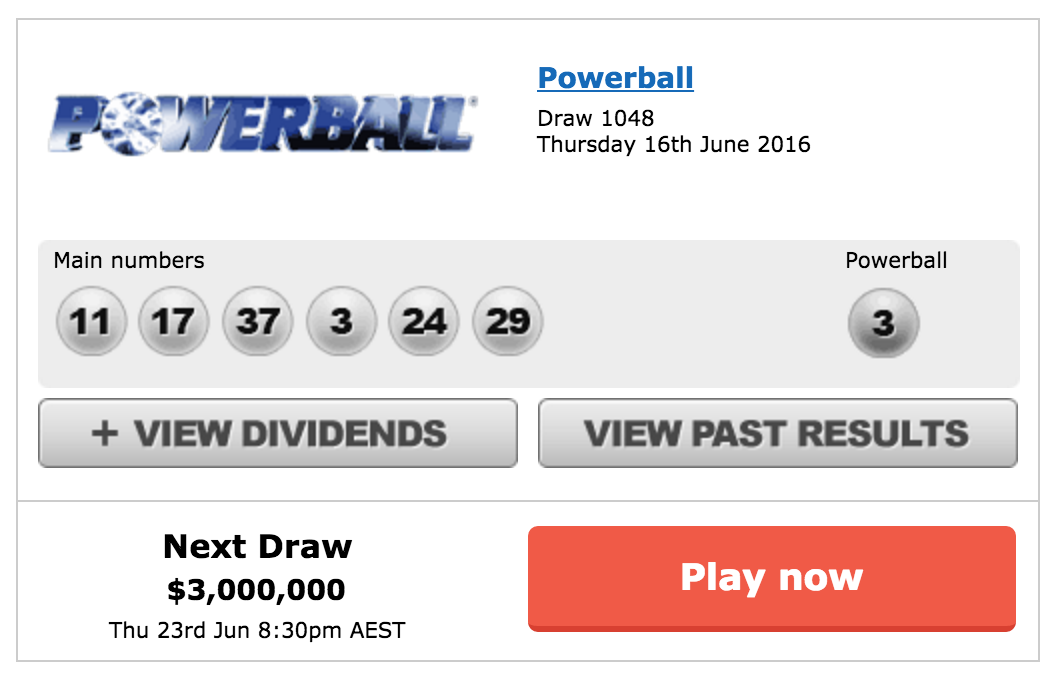
\includegraphics[height=3cm]{../images/Powerball.jpg}
\end{center}
\href{https://tatts.com/goldencasket/games/powerball/how-to-play}{\beamergotobutton{Powerball Rules}}

\end{frame}

\subsection{Example2: Tasmanian fruit flies}
\begin{frame}\frametitle{Example2: Tasmanian Fruit flies}

Tasmania is currently free of fruit fly which adds several million dollars to the annual export income earned by the horticultural industries. However the 14 species of fruit fly on the Australian mainland are a constant economic threat. South Australia remains the only Australian mainland state that is fruit fly free, with prevention, detection and eradication measures costing about \textdollar 5 million annually. 

\begin{center}
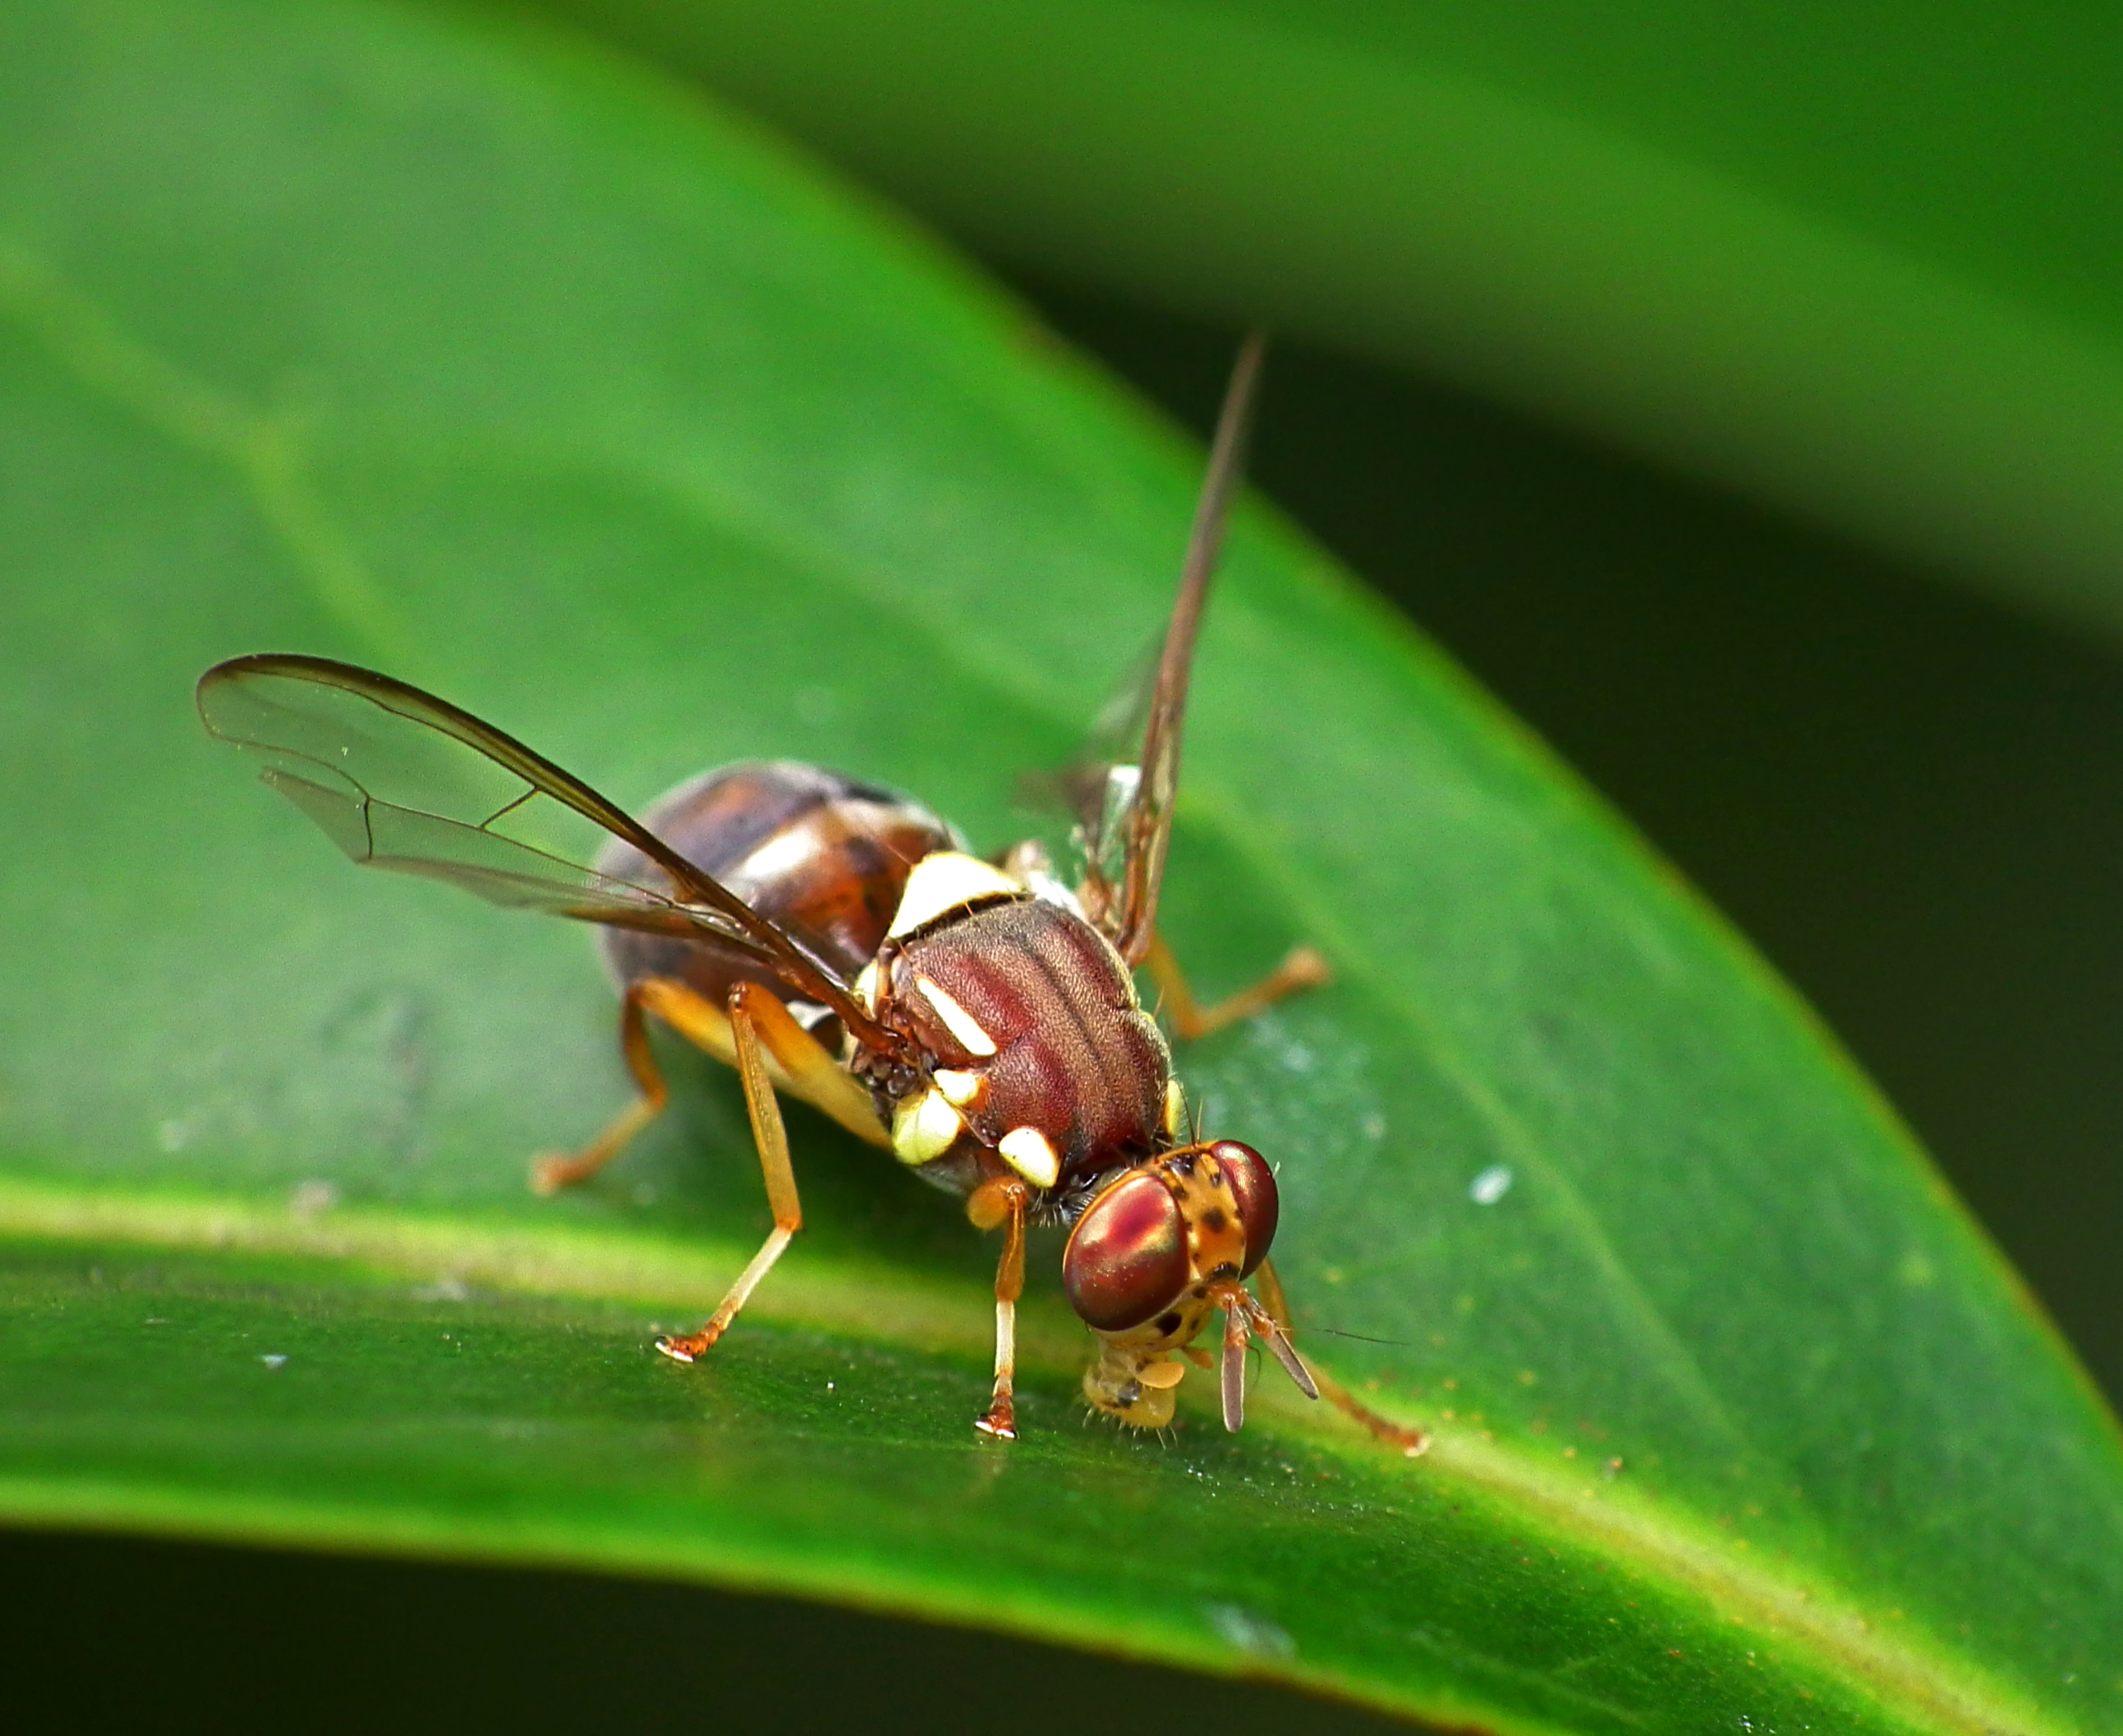
\includegraphics[height=3cm]{../images/Queensland_Fruit_Fly_-_Bactrocera_tryoni.jpg}
\end{center}
\href{http://dpipwe.tas.gov.au/biosecurity/plant-biosecurity/pests-and-diseases/fruit-fly}{\beamergotobutton{TasmaniaGovt}}
\href{http://pir.sa.gov.au/biosecurity/fruit\_fly}{\beamergotobutton{Biosecurity}}
\end{frame}

\begin{frame}\frametitle{}

Suppose there are 100 fruit flies buzzing around a lime tree. The flies have a 20\% chance on landing on the tree and act independently. 

\vspace{.5cm}
{\bf What is the probability that exactly 20 flies land on the lime tree?}

\vspace{1cm}
{\tiny Note: If there were only 2 flies, we could use simple probability.
\begin{itemize}
\item The set of all possible values: $x=0,1,2$.
\item  The likelihood of each value (discrete): \\
$P(X=0) = P(\mbox{no flies land}) = 0.8 \times 0.8 = 0.64$ \\
$P(X=1) = P(\mbox{1 fly lands}) = 0.2 \times 0.8 +  0.8 \times 0.2 = 0.32$ \\
$P(X=2) = P(\mbox{both flies land}) = 0.2^2  = 0.04$ \\
\end{itemize}

But we can't use this approach for a  realistic number of flies, like $n=100$. So we need to develop a general formula for $P(X=x)$.}
\end{frame}


\subsection{Example3: Calcium deficiency in orchards}
\begin{frame}\frametitle{Example3: Calcium deficiency in orchards}

While magnesium deficiency occurs in most districts in New South Wales, calcium deficiency is rarely seen in citrus orchards. A deficient range is below 1.6 percent of dry leaf matter and satisfactory range is 3-5.5.

\vspace{.5cm}
A small size orchard is considering ordering an expensive fertilizer. {\bf What is the chance that more than 1 tree will be calcium deficient?}

\vspace{.5cm}
\href{http://www.dpi.nsw.gov.au/agriculture/horticulture/citrus/management/nutrition/nutrition}{\beamergotobutton{NSW agriculture}}
\end{frame}


\subsection{Discrete Distributions}
\begin{frame}\frametitle{Discrete Distributions}
\begin{definition}[Discrete Distribution]

For any \alert{discrete} distribution $X$, we have a sample space $\Omega$ with values $x= \{ x_{1}, x_{2}, \ldots \}$ and associated probabilities $\{ p_{1}, p_{2} \ldots \}$, where $\{ p_{i} = P(X=x_{i}) \}$.

\vspace{.5cm}
Properties: 
\begin{itemize}
\item there is a countable number of possible values;
\item $\sum_{i} p_{i} = 1$
\end{itemize}
\end{definition}
\end{frame}

\begin{frame}\frametitle{}
\begin{definition}[Probability Distribution Function]
The probability distribution function (or probability distribution) of $X$ is 
the set of \{$x, P(X=x) \}$.
\end{definition}

\vspace{.5cm}
\begin{definition}[Cumulative Distribution Function (CDF)]

The cumulative distribution function (CDF) of $X$ is 
\[ F(x) = P(X \leq x) \]

This is a step function. Statistical tables are often presented in terms of the CDF.
\end{definition}
\end{frame}


\subsection{Mean and Variance of Discrete Distributions}
\begin{frame}\frametitle{The Mean of a Discrete Distribution}

\begin{definition}[Mean or Expectation]
The mean of $X$ is 
\[ \mu = E(X) = \sum_{x} x P(X=x)  \]

\end{definition}

\begin{definition}[Expectation of a Function]

The expectation of $g(X)$ is 
\[ E(g(X)) = \sum_{x} g(x) P(X=x)  \]

For example: $E(X^2) = \sum_{x} x^2 P(X=x) $.

\end{definition}

\end{frame}

\begin{frame}\frametitle{The Variance of a Discrete Distribution}
\begin{definition}[Variance]

The variance of $X$ is 
\[ Var(X) = V(X) =  E(X - \mu)^2 = E(X^2) - E(X)^2  \]
\end{definition}

\end{frame}


\begin{frame}\frametitle{What does the `Mean' mean?}

There are 4 main statistical usages of the word `mean':
\begin{itemize}
\item 
The mean of a sample: $\bar{x}$
\item
The mean of a population: $\mu$
\item
The mean of a random variable $X$ (describing a population): $E(X)$
\item
The distribution of the sampling mean: $\bar{X}$
\end{itemize}

\vspace{.5cm}
Similarly, there are 4 main usages of the word `variance'.

\end{frame}


\begin{frame}\frametitle{Example}
\begin{block}{Mean and variance of 5 tosses of a coin}
Let $X = $ the number of heads in 5 tosses of a coin, $x=0,1,\ldots,5$, with probability distribution function:

\begin{center}
\begin{tabular}{|l|l|l|l|l|l|l|} \hline
$x$ & 0 & 1 & 2 & 3 & 4 & 5  \\ \hline
$P(X=x)$ & $\frac{1}{32}$ & $\frac{5}{32}$ & $\frac{10}{32}$ & $\frac{10}{32}$ & $\frac{5}{32}$ & $\frac{1}{32}$  \\ \hline
\end{tabular}
\end{center}

Find the mean and variance of $X$.
\end{block}
\end{frame}

\begin{frame}\frametitle{}
\begin{alertblock}{}

\[ \mu = E(X) = \sum_{x} x P(X=x) = 0 \times \frac{1}{32} + 1 \times \frac{5}{32} + \ldots  5 \times \frac{1}{32} = 2.5 \]

\[ E(X^2) = \sum_{i} x^2 P(X=x) = 0^2 \times \frac{1}{32} + 1^2 \times \frac{5}{32} + \ldots  5^2 \times \frac{1}{32} = 7.5 \]

Hence
\[ Var(X) = E(X^2) - E(X)^2 = 7.5 - (2.5)^2 = 1.25  \]

\end{alertblock}
\end{frame}

\begin{frame}[fragile]\frametitle{In R}
\begin{knitrout}
\definecolor{shadecolor}{rgb}{0.969, 0.969, 0.969}\color{fgcolor}\begin{kframe}
\begin{alltt}
\hlstd{x}\hlkwb{=}\hlkwd{c}\hlstd{(}\hlnum{0}\hlstd{,}\hlnum{1}\hlstd{,}\hlnum{2}\hlstd{,}\hlnum{3}\hlstd{,}\hlnum{4}\hlstd{,}\hlnum{5}\hlstd{)}
\hlstd{p}\hlkwb{=}\hlkwd{c}\hlstd{(}\hlnum{1}\hlstd{,}\hlnum{5}\hlstd{,}\hlnum{10}\hlstd{,}\hlnum{10}\hlstd{,}\hlnum{5}\hlstd{,}\hlnum{1}\hlstd{)}\hlopt{/}\hlnum{32}
\hlkwd{sum}\hlstd{(x}\hlopt{*}\hlstd{p)}
\end{alltt}
\begin{verbatim}
## [1] 2.5
\end{verbatim}
\begin{alltt}
\hlkwd{sum}\hlstd{(x}\hlopt{^}\hlnum{2}\hlopt{*}\hlstd{p)}
\end{alltt}
\begin{verbatim}
## [1] 7.5
\end{verbatim}
\begin{alltt}
\hlkwd{sum}\hlstd{(x}\hlopt{^}\hlnum{2}\hlopt{*}\hlstd{p)}\hlopt{-}\hlstd{(}\hlkwd{sum}\hlstd{(x}\hlopt{*}\hlstd{p))}\hlopt{^}\hlnum{2}
\end{alltt}
\begin{verbatim}
## [1] 1.25
\end{verbatim}
\begin{alltt}
\hlkwd{sum}\hlstd{((x}\hlopt{-}\hlkwd{sum}\hlstd{(x}\hlopt{*}\hlstd{p))}\hlopt{^}\hlnum{2}\hlopt{*}\hlstd{p)}
\end{alltt}
\begin{verbatim}
## [1] 1.25
\end{verbatim}
\end{kframe}
\end{knitrout}
\end{frame}

\begin{frame}[fragile]\frametitle{}
\begin{alertblock}{Have a try}
In a certain game, 5 coins are tossed, where $X$ denotes the number of heads. It costs \$8.00 to play, and the player receives $\$ 2^X$ as prize money. Show that the expected loss for 1 game is $\$ 0.41$.
\end{alertblock}

\begin{knitrout}
\definecolor{shadecolor}{rgb}{0.969, 0.969, 0.969}\color{fgcolor}\begin{kframe}
\begin{alltt}
\hlcom{#Check your answer}
\hlstd{x}\hlkwb{=}\hlkwd{c}\hlstd{(}\hlnum{0}\hlstd{,}\hlnum{1}\hlstd{,}\hlnum{2}\hlstd{,}\hlnum{3}\hlstd{,}\hlnum{4}\hlstd{,}\hlnum{5}\hlstd{)}
\hlstd{p}\hlkwb{=}\hlkwd{c}\hlstd{(}\hlnum{1}\hlstd{,}\hlnum{5}\hlstd{,}\hlnum{10}\hlstd{,}\hlnum{10}\hlstd{,}\hlnum{5}\hlstd{,}\hlnum{1}\hlstd{)}\hlopt{/}\hlnum{32}
\hlkwd{sum}\hlstd{((}\hlnum{2}\hlopt{^}\hlstd{x)}\hlopt{*}\hlstd{p)}\hlopt{-}\hlnum{8.00}
\end{alltt}
\begin{verbatim}
## [1] -0.40625
\end{verbatim}
\end{kframe}
\end{knitrout}
\end{frame}


\begin{frame}[fragile]{}
\begin{alertblock}{Your Turn}
Suppose you toss a fair coin 1000 times:  when it lands heads
you receive \$1, and when it lands tails you pay me \$1.
What is your expected profit or loss?
\end{alertblock}


\begin{knitrout}
\definecolor{shadecolor}{rgb}{0.969, 0.969, 0.969}\color{fgcolor}\begin{kframe}
\begin{alltt}
\hlstd{x}\hlkwb{=}\hlkwd{c}\hlstd{(}\hlnum{1}\hlstd{,}\hlopt{-}\hlnum{1}\hlstd{)}
\hlstd{p}\hlkwb{=}\hlkwd{c}\hlstd{(}\hlnum{0.5}\hlstd{,}\hlnum{0.5}\hlstd{)}
\hlkwd{sum}\hlstd{(x}\hlopt{*}\hlstd{p)}
\end{alltt}
\begin{verbatim}
## [1] 0
\end{verbatim}
\end{kframe}
\end{knitrout}
\end{frame}


\subsection{Example1: Hypergeometric Distribution}

\begin{frame}\frametitle{Common Types of Discrete Distributions}
There are an infinite number of discrete distributions. 

\vspace{0.5cm}
We will concentrate on 2 special examples: 
\begin{itemize}
\item The Hypergeometric Distribution (Urn model);
\item The Binomial Distribution;
\end{itemize}

For your reference, the Poisson Distribution is also considered as an Appendix.
\end{frame}

\begin{frame}[fragile]{Example1: Hypergeometric Distribution}

\begin{definition}[General Hypergeometric Model]
The \alert{Hypergeometric distribution} models a context described by an urn model.

\vspace{.5cm}
Suppose an urn contains $N$ balls, with $N_{1}$ of type 1, $N_{2}$ of type 2, $\ldots$ $N_{k}$ of type $k$, where $\sum_{i=1}^{k} N_{i} = N$.

\vspace{.5cm}
We select a random sample (without replacement) of $n$ balls (where $n \leq N$.)

\vspace{.5cm}
The probability that we select exactly $n_{i}$ of type $i$ is 

\[ P( \mbox{Select $n_{i}$ balls of each type $i$} )   = 
\frac{ { N_{1} \choose n_{1}}  {N_{2} \choose n_{2}} \ldots {N_{k} \choose n_{k}}  }{ {N \choose n} }
\]

\end{definition}
\hyperlink{Factorials}{\beamergotobutton{Factorials}}
\hyperlink{BinomialCoefficients}{\beamergotobutton{BinomialCoefficients}}
\end{frame}

\begin{frame}[fragile]{}

\begin{block}{Example (Packet of M \& Ms)}
Suppose a small Christmas packet of M \& Ms contains $16$ chocolates, of which  $10$ are red and $6$ are green. We select a random sample of $3$ chocolates. What is the probability of selecting exactly $2$ red ones?
\end{block}

\begin{center}
\begin{tikzpicture}
\draw [blue] (0,1) rectangle (6.1,2);
\draw [red, fill=red, ultra thick] (0.6,1.5) circle [radius=0.1];;
\draw [red, fill=red, ultra thick] (0.9,1.5) circle [radius=0.1];;
\draw [red, fill=red, ultra thick] (1.2,1.5) circle [radius=0.1];;
\draw [red, fill=red, ultra thick] (1.5,1.5) circle [radius=0.1];;
\draw [red, fill=red, ultra thick] (1.8,1.5) circle [radius=0.1];;
\draw [red, fill=red, ultra thick] (2.1,1.5) circle [radius=0.1];;
\draw [red, fill=red, ultra thick] (2.4,1.5) circle [radius=0.1];;
\draw [red, fill=red, ultra thick] (2.7,1.5) circle [radius=0.1];;
\draw [red, fill=red, ultra thick] (3,1.5) circle [radius=0.1];;
\draw [red, fill=red, ultra thick] (3.3,1.5) circle [radius=0.1];;
\draw [green, fill=green, ultra thick] (4,1.5) circle [radius=0.1];;
\draw [green, fill=green, ultra thick] (4.3,1.5) circle [radius=0.1];;
\draw [green, fill=green, ultra thick] (4.6,1.5) circle [radius=0.1];;
\draw [green, fill=green, ultra thick] (4.9,1.5) circle [radius=0.1];;
\draw [green, fill=green, ultra thick] (5.2,1.5) circle [radius=0.1];;
\draw [green, fill=green, ultra thick] (5.5,1.5) circle [radius=0.1];;

\draw [->, blue, ultra thick]  (3,1) -- (3,0);

\draw [blue, rounded corners=.8ex] (2,-1) rectangle (4,0);
\draw [red, fill=red, ultra thick] (2.3,-0.5) circle [radius=0.1];;
\draw [red, fill=red, ultra thick] (2.6,-0.5) circle [radius=0.1];;
\draw [green, fill=green, ultra thick] (3.3,-0.5) circle [radius=0.1];;
\end{tikzpicture}
\end{center}

The probability that we select exactly $n=2$ red balls is
\[ \frac{ { 10 \choose 2}  {6 \choose 1}  }{ {16 \choose 3} } \approx 0.48 \]

\end{frame}

\begin{frame}[fragile]{}
\begin{knitrout}
\definecolor{shadecolor}{rgb}{0.969, 0.969, 0.969}\color{fgcolor}\begin{kframe}
\begin{alltt}
\hlkwd{choose}\hlstd{(}\hlnum{10}\hlstd{,}\hlnum{2}\hlstd{)}\hlopt{*}\hlkwd{choose}\hlstd{(}\hlnum{6}\hlstd{,}\hlnum{1}\hlstd{)}\hlopt{/}\hlkwd{choose}\hlstd{(}\hlnum{16}\hlstd{,}\hlnum{3}\hlstd{)}
\end{alltt}
\begin{verbatim}
## [1] 0.4821429
\end{verbatim}
\end{kframe}
\end{knitrout}

\begin{knitrout}
\definecolor{shadecolor}{rgb}{0.969, 0.969, 0.969}\color{fgcolor}\begin{kframe}
\begin{alltt}
\hlkwd{dhyper}\hlstd{(}\hlnum{2}\hlstd{,}\hlnum{10}\hlstd{,}\hlnum{6}\hlstd{,}\hlnum{3}\hlstd{)}   \hlcom{# dhyper(x,N1,N2,n)}
\end{alltt}
\begin{verbatim}
## [1] 0.4821429
\end{verbatim}
\end{kframe}
\end{knitrout}

\end{frame}

\begin{frame}[fragile]{}
\begin{block}{Example (Powerball)}
What is the probability of winning Powerball (Division 1)?  
\end{block}

\begin{knitrout}
\definecolor{shadecolor}{rgb}{0.969, 0.969, 0.969}\color{fgcolor}\begin{kframe}
\begin{alltt}
\hlstd{(}\hlkwd{choose}\hlstd{(}\hlnum{6}\hlstd{,}\hlnum{6}\hlstd{)}\hlopt{*}\hlkwd{choose}\hlstd{(}\hlnum{34}\hlstd{,}\hlnum{0}\hlstd{)}\hlopt{/}\hlkwd{choose}\hlstd{(}\hlnum{40}\hlstd{,}\hlnum{6}\hlstd{))}\hlopt{*}
  \hlstd{(}\hlkwd{choose}\hlstd{(}\hlnum{1}\hlstd{,}\hlnum{1}\hlstd{)}\hlopt{*}\hlkwd{choose}\hlstd{(}\hlnum{19}\hlstd{,}\hlnum{0}\hlstd{)}\hlopt{/}\hlkwd{choose}\hlstd{(}\hlnum{20}\hlstd{,}\hlnum{1}\hlstd{))}
\end{alltt}
\begin{verbatim}
## [1] 1.302633e-08
\end{verbatim}
\end{kframe}
\end{knitrout}

\begin{knitrout}
\definecolor{shadecolor}{rgb}{0.969, 0.969, 0.969}\color{fgcolor}\begin{kframe}
\begin{alltt}
\hlkwd{dhyper}\hlstd{(}\hlnum{6}\hlstd{,}\hlnum{6}\hlstd{,}\hlnum{34}\hlstd{,}\hlnum{6}\hlstd{)}\hlopt{*}\hlkwd{dhyper}\hlstd{(}\hlnum{1}\hlstd{,}\hlnum{1}\hlstd{,}\hlnum{19}\hlstd{,}\hlnum{1}\hlstd{)}
\end{alltt}
\begin{verbatim}
## [1] 1.302633e-08
\end{verbatim}
\end{kframe}
\end{knitrout}

\vspace{.5cm}
Does this match the claim on the powerball website?
`The chance of winning a Division One prize in Powerball is 1 in 76,767,600'.
\href{https://www.ozlotteries.com/play/powerball}{\beamergotobutton{Powerball Rules}}

\end{frame}

\subsection{Example2: Binomial Distribution}
\begin{frame}\frametitle{Example2: Binomial Distribution}
\begin{definition}[Binomial Distribution]
The \alert{Binomial distribution} models a context in which we have:
\begin{itemize}
\item a fixed number $n$ of independent Binary trials; 
\item  a fixed likelihood of a success at each trial $p=P(\mbox{success})$. 
\end{itemize}

\vspace{.5cm}
If $X =$ the number of successes in $n$ trials, then  $X \sim Bin(n,p)$ with
\[ P(X=x) = {n \choose x} p^x (1-p)^{n-x} \hspace{1cm} \mbox{for } x=0,1,2,\ldots,n. \]
\end{definition}

\vspace{.5cm}
Note:  $\sim$ reads `is distributed as'.
\hyperlink{Factorials}{\beamergotobutton{Factorials}}
\hyperlink{BinomialCoefficients}{\beamergotobutton{BinomialCoefficients}}
\end{frame}

\begin{frame}
Notes:
\begin{itemize}
\item A {\it Binary} (or Bernoulli) trial is an event where there can only be 2 options: success or failure. For example, 1 fruit fly is buzzing around a fruit tree: will it land or not?
\item {\it Success} designates the event we are interested in counting, which may not be good. For example,  $p=P(\mbox{fruit fly lands on fruit tree})$.
\item The Binomial distribution has 2 parameters: $n$ and $p$. Parameters represent the numerical inputs needed for the model.
\item It can be shown (by algebra) that the Binomial distribution has mean $E(X)=np$ and variance $Var(X)=np(1-p)$.
\end{itemize}
\end{frame}

\begin{frame}[fragile]\frametitle{Example of Binomial Distribution with changing $p$}

$X \sim Bin(n=20,p)$, for different $p=0.1,0.2,\ldots ,1$. \\

\vspace{0.5cm}
\begin{knitrout}
\definecolor{shadecolor}{rgb}{0.969, 0.969, 0.969}\color{fgcolor}
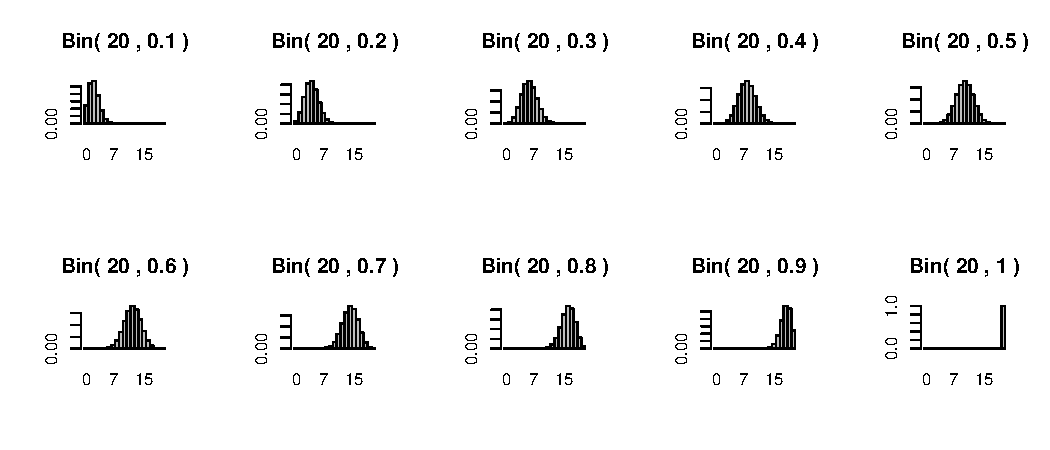
\includegraphics[width=\maxwidth]{figure/unnamed-chunk-69-1} 

\end{knitrout}

\end{frame}



\begin{frame}\frametitle{Example}
\begin{block}{Fruit Flies}
There are 10 fruit flies buzzing around a lime tree. The flies have a 20\% chance on landing on the tree and act independently.
If $X$ represents the number of flies that land on the tree, what is the distribution of $X$?  What is the chance that no flies land on the tree? What is the chance that less than 2 flies land on the tree? 

\vspace{.5cm}
\begin{enumerate}
\item Identify the model: \\
$X = \mbox{the number of flies that land} \sim Bin(n,p)$, where
$n= \mbox{number of flies} = 10$;
$p=P(\mbox{fruit fly lands}) =0.2$.
\item  
Calculate probability:\\
$P(\mbox{no flies land}) = P(X=0) = {10 \choose 0} (0.2)^0 (0.8)^{10} = \frac{10!}{0! (10-0)!} (0.8)^{10} =(0.8)^{10} \approx 0.11$.
\end{enumerate}
\end{block}
\end{frame}


\begin{frame}[fragile]\frametitle{}
\begin{block}{}
Calculate probability:  \\
$P(\mbox{less than 2 flies land}) = P(X \leq 1) = P(X=0) +P(X=1) = 0.1073742 + {10 \choose 1} (0.2)^1 (0.8)^9 \approx 0.38$.
\end{block}

\begin{knitrout}
\definecolor{shadecolor}{rgb}{0.969, 0.969, 0.969}\color{fgcolor}\begin{kframe}
\begin{alltt}
\hlcom{# dbinom(x,n,p) calculates P(X=x) for Bin(n,p)}
\hlkwd{dbinom}\hlstd{(}\hlnum{0}\hlstd{,}\hlnum{10}\hlstd{,}\hlnum{0.2}\hlstd{)}
\end{alltt}
\begin{verbatim}
## [1] 0.1073742
\end{verbatim}
\end{kframe}
\end{knitrout}

\begin{knitrout}
\definecolor{shadecolor}{rgb}{0.969, 0.969, 0.969}\color{fgcolor}\begin{kframe}
\begin{alltt}
\hlcom{# pbinom(x,n,p) calculates P(X<=x) for Bin(n,p)}
\hlkwd{pbinom}\hlstd{(}\hlnum{1}\hlstd{,}\hlnum{10}\hlstd{,}\hlnum{0.2}\hlstd{)}
\end{alltt}
\begin{verbatim}
## [1] 0.3758096
\end{verbatim}
\end{kframe}
\end{knitrout}
\end{frame}


\subsection{Appendix: Poisson Distribution}
\begin{frame}\frametitle{Appendix: Poisson Distribution}

The Poisson distribution is used in 2nd year courses, so is given here for reference.

\begin{definition}[Poisson Distribution]
The \alert{Poisson distribution} models a context in which we have
\begin{itemize}
\item events occuring in an interval; 
\item the average number of events occuring in an interval is $\lambda$ (rate).
\end{itemize}

\vspace{.5cm}
If $X =$ number of events in the interval, then $X \sim Po(\lambda)$ and

\[ P(X=x) =   \frac{ \lambda^x e^{-\lambda}}{x!} 
\hspace{1cm} \mbox{for } x=0,1,2,\ldots \mbox{ and } \lambda > 0. \]
\end{definition}
\end{frame}

\begin{frame}
Notes:
\begin{itemize}
\item $\lambda$ is pronounced `lambda'.
\item Poisson is pronounced `pwasonn'.
\item The Poisson distribution has 1 parameter: $\lambda$.
\item 
The Poisson Distribution models rare events, where $\lambda$ is small.

For example, $\lambda=$ the average number of lime trees exhibiting calcium deficiency in an orchard in a year.
\item It can be shown (by algebra) that the Poisson distribution has mean $E(X)=Var(X)=\lambda.$
\end{itemize}

\vspace{.5cm}
Extension: For large $n$ and small $p$, $X \sim Bin(n,p)$ can be approximated by $Y \sim Po(\lambda=np)$.
\end{frame}

\begin{frame}[fragile]\frametitle{Examples of Poisson Distributions with changing $\lambda$}

$X \sim P_{0}(\lambda)$, for different $\lambda=1,0.2,\ldots 10$. \\

\vspace{0.5cm}
\begin{knitrout}
\definecolor{shadecolor}{rgb}{0.969, 0.969, 0.969}\color{fgcolor}
\includegraphics[width=\maxwidth]{figure/unnamed-chunk-72-1} 

\end{knitrout}
\end{frame}

\begin{frame}\frametitle{Example}
\begin{block}{Magnesium deficiency}

While magnesium deficiency occurs in most districts in New South Wales, calcium deficiency is rarely seen in citrus orchards. A deficient range is below 1.6 percent of dry leaf matter and satisfactory range is 3-5.5.

\vspace{.5cm}
For a small size orchard, let $X$ represent the number of trees with calcium deficiency in a year, where $\lambda=2$.  
For ordering an expensive fertilizer, what is the chance that more than 1 tree will be calcium deficient? 
\href{http://www.dpi.nsw.gov.au/agriculture/horticulture/citrus/management/nutrition/nutrition}{\beamergotobutton{NSW agriculture}}
\end{block}
\end{frame}

\begin{frame}\frametitle{}


\begin{block}{}
\begin{enumerate}
\item Identify the model: \\
$X = \mbox{the number of trees that are calcium deficient} \sim Po(\lambda)$, where 
$\lambda= \mbox{average number of deficient trees in a year} = 2$.
\item  
Calculate probabilities: \\
$P(\mbox{X=0}) = \frac{ 2^0 e^{-2}}{0!} =e^{-2} = 0.1353353$ \\
$P(\mbox{X = 1}) =  \frac{ 2^1 e^{-2}}{1!} = 0.2706706$ \\
$P(X > 1) = 1- P(X=0) - P(X=1) = 0.5939941$
\end{enumerate}
\end{block}
\end{frame}

\begin{frame}[fragile]\frametitle{}
\begin{knitrout}
\definecolor{shadecolor}{rgb}{0.969, 0.969, 0.969}\color{fgcolor}\begin{kframe}
\begin{alltt}
\hlcom{# dpois(x,l) calculates P(X=x) for Po(l)}

\hlkwd{dpois}\hlstd{(}\hlnum{0}\hlstd{,}\hlnum{2}\hlstd{)}
\end{alltt}
\begin{verbatim}
## [1] 0.1353353
\end{verbatim}
\end{kframe}
\end{knitrout}

\begin{knitrout}
\definecolor{shadecolor}{rgb}{0.969, 0.969, 0.969}\color{fgcolor}\begin{kframe}
\begin{alltt}
\hlcom{# ppois(x,l) calculates P(X<=x) for Po(l)}

\hlnum{1}\hlopt{-}\hlkwd{ppois}\hlstd{(}\hlnum{1}\hlstd{,}\hlnum{2}\hlstd{)}
\end{alltt}
\begin{verbatim}
## [1] 0.5939942
\end{verbatim}
\end{kframe}
\end{knitrout}
\end{frame}

  




%%%% TOPIC6 %%%%
\section[6]{Topic6: Continuous Random Variables}
\subsection[Example]{Example: Australian Netball and AFL teams}
\begin{frame}{Example: Australian Netball and AFL teams}

In 2015 the Australian Institute of Sport ran a netball training camp for the best Australian young players playing in goals: shooters, attackers, keepers and defence. All players were over 189cm in height.  

\vspace{.5cm}
`Tall goal shooters and tall goal keepers are much more a part of the scene than when I was playing 15 years ago. We recognise that in Australia the game of netball is changing, we want to remain competitive and maintain a competitive advantage."

(Former Australian netball team member and AIS Centre of Excellence coach Jenny Borlase)
\href{http://www.abc.net.au/news/2015-06-14/tall-athletes-get-support-at-ais-to-stand-as-proud-netballers/6544642}{\beamergotobutton{ABC News}}
\end{frame}



\begin{frame}{}

{\bf What is the probability of finding an Australian woman of `goal player' height or taller?}

\begin{center}
\includegraphics[height=6cm]{../images/NetballHeight.jpg}
\end{center}

\end{frame}


\begin{frame}{}

If $X$ represents the heights of Australian women (in cms), what is $P(X > 189)$?

\vspace{1cm}
\begin{knitrout}
\definecolor{shadecolor}{rgb}{0.969, 0.969, 0.969}\color{fgcolor}
\includegraphics[width=\maxwidth]{figure/unnamed-chunk-76-1} 

\end{knitrout}
\end{frame}



\begin{frame}[fragile]{}

Similarly, in the Australian Football League (AFL) recruiters tend to look for tall male players.

\vspace{.5cm}
'Data collected by Adelaide sports doctor Geoffrey Verrall and AFL sports scientist Jamie Hepner suggest genetics play a bigger part in achieving a top-level football career than skill or desire. Using AFL statistics, they noted the height of the 562 rookies selected in AFL national drafts between 2004 and 2010. They found those shorter than 180cm could just about forget trying for a place in the elite league - unless they happened to be an indigenous or Pacific Islander player, who thrive on leg speed and lightning reflexes ... Generally, white Australian males must be tall (about 188cm) to  make it in the AFL.'
\href{http://www.heraldsun.com.au/sport/afl/size-matters-at-afl-level/story-e6frf9jf-1226650225771}{\beamergotobutton{HeraldSun}}
\end{frame}


\begin{frame}{}

{\bf What proportion of Australian men are similar height to Sydney superstar Adam Goodes (191cm) or West Coast ruckman Nick Naitanui (201cm)?}

\begin{center}
\includegraphics[height=6cm]{../images/NicN.jpg}
\end{center}

\href{http://www.sbs.com.au/news/sites/sbs.com.au.news/files/images/1/5/15Apr_NicNaitanui_800x600.jpg}{\beamergotobutton{SBS}}
\end{frame}


\begin{frame}{}

If $Y$ represents the heights of Australian men (in cms), what is $P(Y > 191)$ or even $P(Y > 201)$?

\vspace{1cm}
\begin{knitrout}
\definecolor{shadecolor}{rgb}{0.969, 0.969, 0.969}\color{fgcolor}
\includegraphics[width=\maxwidth]{figure/unnamed-chunk-77-1} 

\end{knitrout}
\end{frame}


\subsection[Comparing Discrete and Continuous Distributions]{Comparing Discrete and Continuous Distributions}
\begin{frame}\frametitle{Comparing Discrete and Continuous Distributions}

There are 5 fundamental differences between discrete and continuous distributions:

\vspace{.5cm}
\begin{tabular}{|l||l|l|} \hline 
 & Discrete & Continuous \\ \hline \hline
Values & Countable & Infinite \\ \hline
Plot &  Histogram $P(X=x)$ & Smooth curve $f(x)$  \\ 
& probability distribution & probability density \\
& function  & function (pdf)  \\ \hline
$P(X=x)$ & $0 \leq P(X=x) \leq 1 \;\; \forall x$
& $P(X=x)=0 \;\; \forall x$ \\ \hline
Sum of & $\sum_{x} P(X=x) = 1$ & $\int_{x} f(x) dx = 1$ \\
Probabilities & Area of histogram & Area under density \\ \hline
$F(x) = P(X \leq x)$ & $\sum_{y=min(x)}^{x} P(X=y)$
& $\int_{-\infty}^{x} f(y) dy$\\
CDF 
\hyperlink{CDF}{\beamergotobutton{CDF}}
& & \\ \hline
\end{tabular}

%Define CDF.
\end{frame}

\begin{frame}\frametitle{}

For any continuous distribution:

\begin{itemize}
\item
there is an infinite number of possible values;
\item
these values may be within a fixed interval. For example, male human heights (in cm) belong to [54.6,272].
\hyperlink{https://en.wikipedia.org/wiki/Human_height}{\beamergotobutton{Human Heights}}
\item
each of the individual probabilities is 0, ie $P(X=x)=0 \;\; \forall x$. This looks strange at first. However, consider that if we allocate even the smallest amount of probability to each of the infinite values, the probabilities could never sum to 1!
\item
the total of all the probabilites, represented by the area under the probability density function (pdf), must be  1.
\item For a continuous distribution
\[ P(a < X < b) = P(a \leq X \leq b) \] 
This is not generally true for a discrete distribution.
\end{itemize}
\end{frame}


\subsection[Normal Distribution]{Normal Distribution}

\begin{frame}[fragile,label=Normalpdf]\frametitle{Normal Distribution}

\begin{definition}[Normal Distribution]
The \alert{Normal distribution} models a symmetric, bell-shaped variable with 2 parameters mean $\mu$ and variance $\sigma^2$ and points of inflection at $\mu \pm \sigma$. We say the variable $X \sim N(\mu, \sigma^2)$. 

\vspace{.5cm}
The probability density function (pdf) is:
\[ f(x)  =  \frac{1}{  \sqrt{2 \pi \sigma^2}}  e^{   -\frac{ (x-\mu)^2 }{2 \sigma^2  } }
\;\;\;\;\; \mbox{for }  x \in (- \infty, \infty) \]

The cumulative distribution function (CDF) is
\[ F(x) = P(X \leq x) = \int_{-\infty}^{x} f(y) dy \]
\end{definition}

\end{frame}


\begin{frame}[fragile]\frametitle{}

The Normal Distribution is very important because it can approximate many natural phenomemon, like annual rainful (sometimes skewed), humidity, evapotranspiration, heights/weights/length of animals, intelligence, and measurement errors. \\

\vspace{.5cm}
It can also approximate sums of random variables, via the Central Limit Theorem (Topic 7). \\

\vspace{.5cm}
{\bf Does the Normal Distribution approximate the distribution of human heights?}

\end{frame}






\begin{frame}[fragile]

\href{http://www.abs.gov.au/websitedbs/CaSHome.nsf/Home/CensusAtSchool+data+for+Calculators#2012}{\beamergotobutton{Data}}


\begin{knitrout}
\definecolor{shadecolor}{rgb}{0.969, 0.969, 0.969}\color{fgcolor}\begin{kframe}
\begin{alltt}
\hlcom{## data <- read.csv("SchoolCensusHeights.csv")}
\hlkwd{names}\hlstd{(data)}
\end{alltt}
\begin{verbatim}
## [1] "FemaleHeight" "MaleHeight"   "AllHeight"
\end{verbatim}
\begin{alltt}
\hlkwd{par}\hlstd{(}\hlkwc{mfrow}\hlstd{=}\hlkwd{c}\hlstd{(}\hlnum{1}\hlstd{,}\hlnum{3}\hlstd{))}
\hlkwd{hist}\hlstd{(data}\hlopt{$}\hlstd{FemaleHeight)}
\hlkwd{hist}\hlstd{(data}\hlopt{$}\hlstd{MaleHeight)}
\hlkwd{hist}\hlstd{(data}\hlopt{$}\hlstd{AllHeight)}
\end{alltt}
\end{kframe}
\includegraphics[width=\maxwidth]{figure/unnamed-chunk-78-1} 

\end{knitrout}

\end{frame}

\begin{frame}[fragile]

\href{https://vincentarelbundock.github.io/Rdatasets/doc/car/Davis.html}{\beamergotobutton{Data}}

\begin{knitrout}
\definecolor{shadecolor}{rgb}{0.969, 0.969, 0.969}\color{fgcolor}\begin{kframe}
\begin{alltt}
\hlcom{## data <- read.csv("DavisHeights.csv")}
\hlkwd{names}\hlstd{(data)}
\end{alltt}
\begin{verbatim}
## [1] "FemaleWeight" "MaleWeight"   "FemaleHeight" "MaleHeight"  
## [5] "ReportFW"     "ReportMW"     "ReportFH"     "ReportMH"
\end{verbatim}
\begin{alltt}
\hlkwd{par}\hlstd{(}\hlkwc{mfrow}\hlstd{=}\hlkwd{c}\hlstd{(}\hlnum{1}\hlstd{,}\hlnum{2}\hlstd{))}
\hlkwd{hist}\hlstd{(data}\hlopt{$}\hlstd{FemaleHeight)}
\hlkwd{hist}\hlstd{(data}\hlopt{$}\hlstd{ReportFH)}
\end{alltt}
\end{kframe}
\includegraphics[width=\maxwidth]{figure/unnamed-chunk-79-1} 

\end{knitrout}
\end{frame}






\begin{frame}[fragile]

Modelling Australian women's heights by $X \sim N(161.8,6^2)$ and men by $Y \sim N(175.6,7^2)$, we get \\
\href{http://www.abs.gov.au/ausstats/abs@.nsf/0/E11CED5FB86D178ACA257AA30014C059?opendocument
}{\beamergotobutton{ABSData}}


\begin{knitrout}
\definecolor{shadecolor}{rgb}{0.969, 0.969, 0.969}\color{fgcolor}
\includegraphics[width=\maxwidth]{figure/unnamed-chunk-81-1} 

\end{knitrout}
\end{frame}


\subsection[Normal Probabilities]{Normal Probabilities}

\begin{frame}[fragile]\frametitle{Normal Probabilities}

{\bf What is the probability of finding an Australian woman of `goal player' height or taller?} \\

\vspace{.5cm}
If $X \sim N(161.8,6^2)$, what is $P(X > 189)$?


\vspace{1cm}
\begin{knitrout}
\definecolor{shadecolor}{rgb}{0.969, 0.969, 0.969}\color{fgcolor}
\includegraphics[width=\maxwidth]{figure/unnamed-chunk-82-1} 

\end{knitrout}
\end{frame}


\begin{frame}[fragile]\frametitle{}
{\bf Method1: Integrate the pdf} \\

\[ P(X > 189) = \int_{189}^{\infty} \frac{1}{  \sqrt{2 \pi (6^2)}}  e^{   -\frac{ (y-161.8)^2 }{2 (6^2)  } } dy \]


\vspace{1cm}
There is no closed form, but we could Numerical Integration.
\begin{knitrout}
\definecolor{shadecolor}{rgb}{0.969, 0.969, 0.969}\color{fgcolor}\begin{kframe}
\begin{alltt}
\hlstd{f} \hlkwb{<-} \hlkwa{function}\hlstd{(}\hlkwc{x}\hlstd{) \{}\hlkwd{dnorm}\hlstd{(x,}\hlnum{161.8}\hlstd{,}\hlnum{6}\hlstd{)\}}
\hlkwd{integrate}\hlstd{(f,}\hlnum{189}\hlstd{,}\hlnum{200}\hlstd{)}
\end{alltt}
\begin{verbatim}
## 2.902907e-06 with absolute error < 3.2e-20
\end{verbatim}
\end{kframe}
\end{knitrout}
\end{frame}


\begin{frame}[fragile]\frametitle{}

{\bf Method2: Use R}

\begin{knitrout}
\definecolor{shadecolor}{rgb}{0.969, 0.969, 0.969}\color{fgcolor}\begin{kframe}
\begin{alltt}
\hlkwd{pnorm}\hlstd{(}\hlnum{189}\hlstd{,}\hlnum{161.8}\hlstd{,}\hlnum{6}\hlstd{)}  \hlcom{#pnorm(x,mean,sd) }
\end{alltt}
\begin{verbatim}
## [1] 0.9999971
\end{verbatim}
\end{kframe}
\end{knitrout}

\begin{knitrout}
\definecolor{shadecolor}{rgb}{0.969, 0.969, 0.969}\color{fgcolor}
\includegraphics[width=\maxwidth]{figure/unnamed-chunk-85-1} 

\end{knitrout}

Upper Tail probabilities are found from Lower Tail probabilties:
\[ P(X > 189) = 1- P(X \leq 189) = 2.9e-06 \]

\end{frame}




\begin{frame}[fragile]
Notes on using R:
\begin{itemize}
\item
Interval probabilities are found by subtraction:
\[ P( 170 < X \leq 175) = 0.07196146 \]

\begin{knitrout}
\definecolor{shadecolor}{rgb}{0.969, 0.969, 0.969}\color{fgcolor}
\includegraphics[width=\maxwidth]{figure/unnamed-chunk-86-1} 

\end{knitrout}

\begin{knitrout}
\definecolor{shadecolor}{rgb}{0.969, 0.969, 0.969}\color{fgcolor}\begin{kframe}
\begin{alltt}
\hlkwd{pnorm}\hlstd{(}\hlnum{175}\hlstd{,}\hlnum{161.8}\hlstd{,}\hlnum{6}\hlstd{)}\hlopt{-}\hlkwd{pnorm}\hlstd{(}\hlnum{170}\hlstd{,}\hlnum{161.8}\hlstd{,}\hlnum{6}\hlstd{)}
\end{alltt}
\begin{verbatim}
## [1] 0.07196146
\end{verbatim}
\end{kframe}
\end{knitrout}
\end{itemize}
\end{frame}

\begin{frame}[fragile]
\begin{itemize}
\item
For the standard Normal $Z \sim N(0,1)$, we can leave the mean and standard deviation unspecified.

\[ P(Z \leq 0.8)  = 0.7881446 \]

\begin{knitrout}
\definecolor{shadecolor}{rgb}{0.969, 0.969, 0.969}\color{fgcolor}
\includegraphics[width=\maxwidth]{figure/unnamed-chunk-88-1} 

\end{knitrout}

\begin{knitrout}
\definecolor{shadecolor}{rgb}{0.969, 0.969, 0.969}\color{fgcolor}\begin{kframe}
\begin{alltt}
\hlkwd{pnorm}\hlstd{(}\hlnum{0.8}\hlstd{,}\hlnum{0}\hlstd{,}\hlnum{1}\hlstd{)}
\end{alltt}
\begin{verbatim}
## [1] 0.7881446
\end{verbatim}
\begin{alltt}
\hlkwd{pnorm}\hlstd{(}\hlnum{0.8}\hlstd{)}
\end{alltt}
\begin{verbatim}
## [1] 0.7881446
\end{verbatim}
\end{kframe}
\end{knitrout}

\end{itemize}
\end{frame}


\begin{frame}[fragile]\frametitle{}

{\bf Method3: Standardise and use the Standard Normal Tables} 

\vspace{.5cm}
The Standard Normal Tables tabulate the CDF for $Z \sim N(0,1)$. \\

\vspace{.5cm}
\includegraphics[height=6cm]{../images/NormalTableSample.pdf}

\end{frame}


\begin{frame}[fragile]\frametitle{}

For example, $P(Z \leq 0.8) = 0.7881$. \\

\begin{knitrout}
\definecolor{shadecolor}{rgb}{0.969, 0.969, 0.969}\color{fgcolor}
\includegraphics[width=\maxwidth]{figure/unnamed-chunk-90-1} 

\end{knitrout}

\includegraphics[height=5cm]{../images/NormalTableEg1.jpg}
\end{frame}

\begin{frame}\frametitle{}

How do we use the Standard Normal Tables for a general Normal?  \\ 

\vspace{.5cm} 
Every General Normal $X \sim N(\mu, \sigma^2)$ can be transformed into the Standard Normal $Z \sim N(0,1)$. 

\vspace{.5cm} 
\begin{definition}[Standardardising a Normal]
If $X \sim N(\mu, \sigma^2)$ and $Z \sim N(0, 1)$, then \\
$P( X \leq x) = P \Big( \frac{X-\mu}{\sigma} \leq \frac{x-\mu}{\sigma}  \Big)= P \Big( Z \leq \frac{x-\mu}{\sigma}  \Big)$
\end{definition}

\begin{eqnarray*}
P(X > 189) & = & P( \frac{X-161.8}{6} > \frac{189-161.8}{6}) \\
& = & P(Z > 4.533333)  \\
& < & 1-0.9986 \\
& = & 0.0014
\end{eqnarray*}
\end{frame}

\begin{frame}[fragile]\frametitle{}

\includegraphics[height=8cm]{../images/NormalTableEg2.jpg}

\end{frame}


\begin{frame}[fragile]\frametitle{}

Effectively we have found that 
\begin{knitrout}
\definecolor{shadecolor}{rgb}{0.969, 0.969, 0.969}\color{fgcolor}
\includegraphics[width=\maxwidth]{figure/unnamed-chunk-91-1} 

\end{knitrout}
is equivalent to
\begin{knitrout}
\definecolor{shadecolor}{rgb}{0.969, 0.969, 0.969}\color{fgcolor}
\includegraphics[width=\maxwidth]{figure/unnamed-chunk-92-1} 

\end{knitrout}

{\tiny
\begin{knitrout}
\definecolor{shadecolor}{rgb}{0.969, 0.969, 0.969}\color{fgcolor}\begin{kframe}
\begin{alltt}
\hlnum{1}\hlopt{-}\hlkwd{pnorm}\hlstd{(}\hlnum{4.533333}\hlstd{)}
\end{alltt}
\begin{verbatim}
## [1] 2.903009e-06
\end{verbatim}
\end{kframe}
\end{knitrout}
}
\end{frame}



\begin{frame}[fragile]\frametitle{}

{\bf Method4: Appoximate using the Special Percentiles of the Normal Distribution} 

All Normal distributions satisfy the "68\%-95\%-99.7\% Rule. \\

\vspace{.5cm}
\begin{tabular}{|l|l|} \hline
Number of sds $\sigma$ from the Mean $\mu$ & \% of Probability \\ \hline
1 & 68\%  \\
2 & 95\% \\
3 & 99.7\% \\ \hline
\end{tabular}


\begin{knitrout}
\definecolor{shadecolor}{rgb}{0.969, 0.969, 0.969}\color{fgcolor}
\includegraphics[width=\maxwidth]{figure/unnamed-chunk-94-1} 

\end{knitrout}

\end{frame}



\subsection[Normal Percentiles]{Normal Percentiles}
\begin{frame}[fragile]\frametitle{Normal Percentiles (Inverse Probabilities)}

Given $X \sim N(161.8,6^2)$, what is the 90\% percentile for heights of Australian women. \\

\vspace{.5cm}
We need to find $q$ such that $P(X \leq q) = 0.9$.

\begin{knitrout}
\definecolor{shadecolor}{rgb}{0.969, 0.969, 0.969}\color{fgcolor}
\includegraphics[width=\maxwidth]{figure/unnamed-chunk-95-1} 

\end{knitrout}

\begin{knitrout}
\definecolor{shadecolor}{rgb}{0.969, 0.969, 0.969}\color{fgcolor}\begin{kframe}
\begin{alltt}
\hlkwd{qnorm}\hlstd{(}\hlnum{0.9}\hlstd{,}\hlnum{161.8}\hlstd{,}\hlnum{6}\hlstd{)}  \hlcom{#qnorm(%,mean,sd)}
\end{alltt}
\begin{verbatim}
## [1] 169.4893
\end{verbatim}
\end{kframe}
\end{knitrout}
\end{frame}


\subsection[Other Distributions]{Other Continuous Distributions}


\begin{frame}\frametitle{Other Continuous Distributions}

We now consider 3 other continuous distributions which will be used in the Hypothesis Testing part of the course (Topic 8 onwards).

\begin{itemize}
\item Student $T$  (T tests)
\item Fisher's $F$ (Test for equal variance and ANOVA in STAT2)
\item Chi-Squared $\chi^{2}$ (Goodness of Fit Tests)
\end{itemize}

\end{frame}


\begin{frame}\frametitle{Student T}

\begin{definition}[Student T Distribution]
The \alert{Student T distribution} is symmetric and bell-shaped with thicker tails than a Normal. 

\vspace{.5cm}
We say the variable $X \sim t_{n}$, with $n$ degrees of freedom.

\vspace{.5cm}
The pdf is:
\[ f(x)  =  \frac{ \Gamma(\frac{n+1}{2})}  { \sqrt{n \pi} \Gamma(\frac{n}{2})}
(1+ \frac{x^2}{n})^{-\frac{n+1}{2}}
\;\;\;\;\; \mbox{for }  x \in (- \infty, \infty) \]
\hyperlink{Normalpdf}{\beamergotobutton{Compare Normal}} 

\vspace{.5cm}
The mean is 0 and variance is $\frac{n}{n-2}$ for $n > 2$.

\end{definition}
\end{frame}

\begin{frame}[fragile]\frametitle{}

\begin{knitrout}
\definecolor{shadecolor}{rgb}{0.969, 0.969, 0.969}\color{fgcolor}
\includegraphics[width=\maxwidth]{figure/unnamed-chunk-97-1} 

\end{knitrout}
\end{frame}
 

\begin{frame}\frametitle{Chi-Squared distribution}

\vspace{.5cm}
\begin{definition}[Chi-Squared distribution]
The \alert{Chi-Squared distribution} is the sum of squared independent Standard Normal random variables. It can only take positive values and typically right skewed.

\vspace{.5cm}
We say the variable $X \sim \chi^2_{n}$, with $n$ degrees of freedom.

\vspace{.5cm}
The pdf is:
\[ f(x)  =  \frac{ 1}  { 2^{\frac{n}{2}} \Gamma(\frac{n}{2})}
x^{\frac{n}{2}-1} e^{-\frac{x}{2}}
\;\;\;\;\; \mbox{for }  x \in (0, \infty) \]

\vspace{.5cm}
The mean is $n$ and variance is $2 n$.
\end{definition}

\end{frame}



\begin{frame}[fragile]\frametitle{}
\begin{knitrout}
\definecolor{shadecolor}{rgb}{0.969, 0.969, 0.969}\color{fgcolor}
\includegraphics[width=\maxwidth]{figure/unnamed-chunk-98-1} 

\end{knitrout}

\end{frame}


\begin{frame}\frametitle{Fisher's F}

\begin{definition}[Fisher's F Distribution]
The \alert{Fisher's F distribution} is the scaled ratio of 2 $\chi^2$ variables, with $m$ and $n$ degrees of freedom.

\vspace{.5cm}
We say the variable $X \sim F_{m,n}$. \\

\vspace{.5cm}
The pdf is:
\[ f(x)  =  \frac{ \Gamma( \frac{m+n}{2} ) m^{\frac{m}{2}}  n^{\frac{n}{2}}   }{ \Gamma( \frac{m}{2} )  \Gamma( \frac{n}{2} )}
\frac{ x^{\frac{m}{2}-1}  }{ (n + mx)^{\frac{m+n}{2}}      }
\;\;\;\;\; \mbox{for }  x \in (0, \infty) \]



\vspace{.5cm}
The mean is $\frac{n}{n-2}$ for $n >2$ and variance is $\frac{2 n^2 (m+n-2)}{m (n-2)^2(n-4)}$ for $n > 4$.



\end{definition}

\end{frame}


\begin{frame}[fragile]\frametitle{}

\begin{knitrout}
\definecolor{shadecolor}{rgb}{0.969, 0.969, 0.969}\color{fgcolor}
\includegraphics[width=\maxwidth]{figure/unnamed-chunk-99-1} 

\end{knitrout}
\end{frame}


\begin{frame}[fragile]\frametitle{}
 
Using commands in R: \\

$P(X \leq 2)$, where $X \sim t_{4}$.

\begin{knitrout}
\definecolor{shadecolor}{rgb}{0.969, 0.969, 0.969}\color{fgcolor}\begin{kframe}
\begin{alltt}
\hlkwd{pt}\hlstd{(}\hlnum{2}\hlstd{,}\hlnum{4}\hlstd{)}
\end{alltt}
\begin{verbatim}
## [1] 0.9419417
\end{verbatim}
\end{kframe}
\end{knitrout}

$P(X \geq 3)$, where $X \sim \chi^2_{4}$.

\begin{knitrout}
\definecolor{shadecolor}{rgb}{0.969, 0.969, 0.969}\color{fgcolor}\begin{kframe}
\begin{alltt}
\hlnum{1}\hlopt{-}\hlkwd{pchisq}\hlstd{(}\hlnum{3}\hlstd{,}\hlnum{4}\hlstd{)}
\end{alltt}
\begin{verbatim}
## [1] 0.5578254
\end{verbatim}
\end{kframe}
\end{knitrout}

$P(1 < X \leq 3)$, where $X \sim F(2,4)$.

\begin{knitrout}
\definecolor{shadecolor}{rgb}{0.969, 0.969, 0.969}\color{fgcolor}\begin{kframe}
\begin{alltt}
\hlkwd{pf}\hlstd{(}\hlnum{3}\hlstd{,}\hlnum{2}\hlstd{,}\hlnum{4}\hlstd{)}\hlopt{-}\hlkwd{pf}\hlstd{(}\hlnum{1}\hlstd{,}\hlnum{2}\hlstd{,}\hlnum{4}\hlstd{)}
\end{alltt}
\begin{verbatim}
## [1] 0.2844444
\end{verbatim}
\end{kframe}
\end{knitrout}

\end{frame}

\begin{frame}[fragile]\frametitle{Summary Examples}

\begin{alertblock}{Have a go}
Dharshani Sivalingam is the tallest netball player in the world. What is the probability of finding an Australian woman of Dharshani’s height?

\href{http://www.thetallestman.com/dharshanisivalingam.htm}{\beamergotobutton{Dharshani}}
\end{alertblock}

\begin{knitrout}
\definecolor{shadecolor}{rgb}{0.969, 0.969, 0.969}\color{fgcolor}\begin{kframe}
\begin{alltt}
\hlcom{#Check your answer}
\hlstd{d}\hlkwb{=}\hlstd{(}\hlnum{208.3} \hlopt{-} \hlnum{161.8}\hlstd{)}\hlopt{/}\hlnum{6}
\hlkwd{pnorm}\hlstd{(d)}
\end{alltt}
\begin{verbatim}
## [1] 1
\end{verbatim}
\end{kframe}
\end{knitrout}

\begin{center}
\includegraphics[height=2cm]{../images/Dharshani.jpg}
\end{center}

\end{frame}

\begin{frame}[fragile]\frametitle{}

\begin{alertblock}{Have a go}
Madison Robinson is the shortest Australian International player. What percentage of Australian women are between Madison and Dharshani’s heights?

\href{https://en.wikipedia.org/wiki/Madison Robinson}{\beamergotobutton{Madison}}

\end{alertblock}

\begin{knitrout}
\definecolor{shadecolor}{rgb}{0.969, 0.969, 0.969}\color{fgcolor}\begin{kframe}
\begin{alltt}
\hlcom{#Check your answer}
\hlstd{m}\hlkwb{=}\hlstd{(}\hlnum{168} \hlopt{-} \hlnum{161.8}\hlstd{)}\hlopt{/}\hlnum{6}
\hlkwd{pnorm}\hlstd{(d)}\hlopt{-}\hlkwd{pnorm}\hlstd{(m)}
\end{alltt}
\begin{verbatim}
## [1] 0.150724
\end{verbatim}
\end{kframe}
\end{knitrout}

\end{frame}


\begin{frame}[fragile]\frametitle{}

\begin{alertblock}{Have a go}
If 60\% of Australian women are below a certain height, what is that height?
\end{alertblock}

\begin{knitrout}
\definecolor{shadecolor}{rgb}{0.969, 0.969, 0.969}\color{fgcolor}\begin{kframe}
\begin{alltt}
\hlcom{#Check your answer}
\hlkwd{qnorm}\hlstd{(}\hlnum{0.6}\hlstd{,}\hlnum{161.8}\hlstd{,}\hlnum{6}\hlstd{)}
\end{alltt}
\begin{verbatim}
## [1] 163.3201
\end{verbatim}
\end{kframe}
\end{knitrout}
\end{frame}

\begin{frame}[fragile]\frametitle{}

\begin{alertblock}{Have a go}
If $X \sim N(8,16)$ find $P(X \leq 20)$.

\end{alertblock}

\begin{knitrout}
\definecolor{shadecolor}{rgb}{0.969, 0.969, 0.969}\color{fgcolor}\begin{kframe}
\begin{alltt}
\hlcom{#Check your answer}
\hlkwd{pnorm}\hlstd{(}\hlnum{20}\hlstd{,}\hlnum{8}\hlstd{,}\hlnum{4}\hlstd{)}
\end{alltt}
\begin{verbatim}
## [1] 0.9986501
\end{verbatim}
\begin{alltt}
\hlkwd{pnorm}\hlstd{(}\hlnum{3}\hlstd{)}
\end{alltt}
\begin{verbatim}
## [1] 0.9986501
\end{verbatim}
\end{kframe}
\end{knitrout}

\end{frame}


\begin{frame}[fragile]\frametitle{}

\begin{alertblock}{Have a go}
Given Australian male heights can be approximated by $X \sim N(175.6,7^2)$, what proportion of Australian man are similar height to Sydney superstar Adam Goodes (191cm) or West Coastruckman Nick Naitanui (201cm)?

\end{alertblock}

\begin{knitrout}
\definecolor{shadecolor}{rgb}{0.969, 0.969, 0.969}\color{fgcolor}\begin{kframe}
\begin{alltt}
\hlcom{#Check your answer}
\hlstd{a} \hlkwb{=} \hlstd{(}\hlnum{191}\hlopt{-}\hlnum{175.6}\hlstd{)}\hlopt{/}\hlnum{7}
\hlnum{1}\hlopt{-} \hlkwd{pnorm}\hlstd{(a)}
\end{alltt}
\begin{verbatim}
## [1] 0.01390345
\end{verbatim}
\begin{alltt}
\hlstd{n} \hlkwb{=} \hlstd{(}\hlnum{201}\hlopt{-}\hlnum{175.6}\hlstd{)}\hlopt{/}\hlnum{7}
\hlnum{1}\hlopt{-} \hlkwd{pnorm}\hlstd{(n)}
\end{alltt}
\begin{verbatim}
## [1] 0.000142497
\end{verbatim}
\end{kframe}
\end{knitrout}
\end{frame}






%%%% TOPIC7 %%%%
\section[7]{Topic7: Combinations of Random Variables}

\subsection[Example: Luggage Limits on A380 Flight]{Example: Luggage Limits on A380 Qantas Flight}

\begin{frame}[fragile]{Example: Luggage Limits on A380 Flight}

When booking flights, explicit luggage limits are specified, and bags are weighed at check-in. For example, for most International flights, the economy checked bag allowance is 30kg. This is essential for the safety and efficiency of the flight, as each plane has a maximum PayLoad (maximum weight allowed for passengers, crew, luggage and cargo).
\href{http://www.qantas.com/travel/airlines/checked-baggage/global/en#international-flights-excluding-north-and-south-america}{\beamergotobutton{QantasCheckedLuggageLimits}}

\begin{center}
\includegraphics[height=4cm]{../images/A380.jpg}
\end{center}
\end{frame}



\begin{frame}{}

For the popular A380 plane, the Operational Weight is 270,000kg and the Zero Fuel Weight is 361,000, giving a maximum PayLoad of 91,000.
\href{hthttps://en.wikipedia.org/wiki/Airbus_A380}{\beamergotobutton{A380}}
\href{http://aviation.stackexchange.com/questions/1008/what-is-the-weight-budget-of-a-fully-loaded-a380}{\beamergotobutton{A380Specs}}

\vspace{.5cm}
{\bf What is the expected PayLoad for 530 passengers and 25 crew? Should passengers be weighed? Should hand luggage be weighted? Is it better to give a maximum luggage limit or specify limits for individual items? What baggage limits would you suggest?}

\vspace{.5cm}
Overbooking of passengers on intercontinental flights is a common practice among airlines. Aircraft which are capable of carrying 300 passengers are booked to carry 320 passengers. 

\vspace{.5cm}
{\bf If 10\% of passengers who have a booking fail
to turn up for their flights, what is the probability that at least one passenger
who has a booking, will end up without a seat on a particular flight?}

\end{frame}


\subsection[Linear Function]{Linear Function of a Random Variable}
\begin{frame}{Linear Function of a Random Variable}
\begin{definition}[Linear Function of Random Variable]
Given a random variable $X$, then $Y = a + b X$ has moments
\[ \boxed{ E(Y) = a + b E(X) } \]
and
\[ \boxed{ Var(Y) = b^2 Var(X) } \]
for all 2 constants $a$ and $b$.

\vspace{.5cm}
Special Case:
If $X \sim N(\mu, \sigma^2)$, then $Y \sim N(a + b \mu, b^2 \sigma^2)$. 

\end{definition}

Notes:  \\
(1) Expectation retains linearity. \\
(2) `A linear function of a Normal is a Normal'. This is the reason that we can standardise a Normal.
\end{frame}

\begin{frame}[fragile]\frametitle{}

\begin{block}{Example: Linear Function}
Suppose the weight of an Australian women $W \sim N(71.1, 12^2)$.
\href{http://www.abs.gov.au/ausstats/abs@.nsf/0/E11CED5FB86D178ACA257AA30014C059?opendocument}{\beamergotobutton{AustralianWeights}} \\
Find the distribution of the weight of an Australian women in pounds, given 1kg = 1 pound/2.2046.
\end{block}

\vspace{.5cm}
Let $P = \mbox{Weight of an Australian women in pounds} = 2.2406 W$. \\

This is a linear function where $a=0$ and $b= 2.2406$. \\

Hence 
\[ E(P) = 0 + 2.2406 E(W) = 2.2406 \times 71.1 =  159.3067 \]
\[ Var(P) = 2.2406^2 Var(W) = 2.2406^2 \times 12^2 = 722.9215 \]
So $P \sim N(159.3067, 26.8872^2)$
\end{frame}




\subsection[Independence]{Independence of Random Variables}

\begin{frame}{}
\begin{definition}[Independence for Random Variables]
For any random variables $X$ and $Y$, we say that \\
$X$ and $Y$ are independent
iff
\[ P(X \leq x, Y \leq y) = P(X \leq x) P(Y \leq y) \]
i.e. the joint CDF splits into the 2 individual CDFs.
\end{definition}

\vspace{.5cm}
Notes: \\
(1) 
It follows that if $X$ and $Y$ are independent, then $Cov(X,Y) = E(XY) - E(X)E(Y) = 0$. However the inverse is not true. \\
(2) You will not need to justify independence. Rather it will be assumed in any question requiring it. \\
(3) Compare to set independence:
\hyperlink{Setindependence}{\beamergotobutton{Set Independence}}
\end{frame}





\subsection[Sums]{Sums of Random Variables}

\begin{frame}{Sums of Random Variables}
\begin{definition}[Total of Random Variables]
Given any sequence of random variables $X_{1}, X_{2}, \ldots, X_{n}$, \\

the total $T = \sum_{i=1}^{n} X_{i}$ has moments
\[ \boxed{ E(T) = \sum_{i=1}^{n} E(X_{i})  } \]
and assuming independence,
\[ \boxed{ Var(T) = \sum_{i=1}^{n} Var(X_{i}) } \]

\end{definition}
\end{frame}

\begin{frame}{}
\begin{definition}[Sample Mean of Random Variables]
Given any sequence of random variables $X_{1}, X_{2}, \ldots, X_{n}$, \\

the sample mean $\bar{X} = \frac{1}{n} \sum_{i=1}^{n} X_{i}$ has moments
\[ \boxed{ E(\bar{X}) = \frac{1}{n} \sum_{i=1}^{n} E(X_{i}) } \]
and assuming independence,
\[ \boxed{ Var(\bar{X}) = \frac{1}{n^2} \sum_{i=1}^{n} Var(X_{i}) } \]
\end{definition}

These are nice results are not very useful when we don't know the shape of distribution. Hence, we will concentrate on sums of {\it Normal} random variables.
\end{frame}




\subsection[NormalSums]{Sums of Normal Random Variables}
\begin{frame}{Sums of Normal Random Variables}
\begin{definition}[Total and Sample Mean of Normal RVs]
Given a sequence of random variables $X_{i} \sim N(\mu_{i}, \sigma_{i}^2)$
(for $i=1,2\ldots,n$) \\

then  \[ \boxed{  T = \sum_{i=1}^{n} X_{i}  \sim N( \sum_{i=1}^{n} \mu_{i}, \sum_{i=1}^{n} \sigma_{i}^2    ) } \]

and
\[ \boxed{  \bar{X} = \frac{1}{n} \sum_{i=1}^{n} X_{i}  \sim N( \frac{1}{n} \sum_{i=1}^{n} \mu_{i}, \frac{1}{n^2} \sum_{i=1}^{n} \sigma_{i}^2  ) } \]

Summary: for constants $a_{i}$,
\[  \boxed{ T = \sum_{i=1}^{n}  a_{i} X_{i}  \sim N( \sum_{i=1}^{n} a_{i} \mu_{i}, \sum_{i=1}^{n} a_{i}^2
\sigma_{i}^2 ) } \]

\end{definition}
\end{frame}


\begin{frame}[fragile]\frametitle{}

\begin{block}{Example: Total}
Suppose the weight of an Australian women is $W \sim N(71.1, 12^2)$, a carry on bag is $C \sim N(6.9,0.5^2)$ and a handbag is $H \sim N(1.3, 0.4^2)$.
\href{http://www.qantas.com./travel/airlines/carry-on-baggage/global/en#carry-on-baggage-allowances}{\beamergotobutton{QantasCarryonLuggage}} \\

Find the probability that the total weight of an Australian woman with carry on luggage is more than 100kg.
\end{block}

\vspace{.5cm}
Let $T = \mbox{Total Weight of a woman with carry on luggage}$. \\

This is a sum of 3 random variables, $T = W + C + H$.

Hence 
\[ E(T) = E(W) + E(C) + E(H) = 71.1 + 6.9 + 1.3 = 79.3 \]
\[ Var(T) =  Var(W) + Var(C) + Var(H) = 12^2 + .5^2 + .4^2 = 144.41 \]
So $T \sim N(79.3, 144.41) = T \sim N(79.3, 12.01707^2)$
\end{frame}


\begin{frame}[fragile]\frametitle{}

So using standardising (Topic 6),

\[ P(T > 100) = P(\frac{T-79.3}{12.01707} > \frac{100-79.3}{12.01707}) = P(Z > 1.72255) \approx 0.04 \]

\begin{knitrout}
\definecolor{shadecolor}{rgb}{0.969, 0.969, 0.969}\color{fgcolor}\begin{kframe}
\begin{alltt}
\hlnum{1}\hlopt{-}\hlkwd{pnorm}\hlstd{(}\hlnum{100}\hlstd{,}\hlnum{79.3}\hlstd{,}\hlnum{12.01707}\hlstd{)}
\end{alltt}
\begin{verbatim}
## [1] 0.042485
\end{verbatim}
\begin{alltt}
\hlnum{1}\hlopt{-}\hlkwd{pnorm}\hlstd{(}\hlnum{1.72255}\hlstd{)}
\end{alltt}
\begin{verbatim}
## [1] 0.04248497
\end{verbatim}
\end{kframe}
\end{knitrout}
\end{frame}


\begin{frame}{}
\begin{definition}[Total and Sample Mean of iid Normal RVs]
Given a sequence of iid random variables $X_{i} \sim N(\mu, \sigma^2)$
(for $i=1,2\ldots,n$) \\

then  \[  \boxed{ T = \sum_{i=1}^{n} X_{i}  \sim N( n \mu , n \sigma^2  ) } \]

and
\[  \boxed{ \bar{X} = \frac{1}{n} \sum_{i=1}^{n} X_{i}  \sim N( \mu, \frac{\sigma^2}{n} ) } \]

\end{definition}
\end{frame}


\begin{frame}[fragile]\frametitle{}

\begin{block}{Example: Sample Mean}
Find the probability that the average weight of 10 Australian women with carry on luggage is more than 100kg.
\end{block}

\vspace{.5cm}
We have already worked out that 1 woman has a total carry on weight of $T \sim N(79.3, 12.01707^2)$. \\

\vspace{.5cm}
Now change the notation and consider a sequence of 10 women: $X_{1}, X_{2}, \ldots, X_{10}$ where $X_{i} = \mbox{carry on weight} \sim N(79.3, 12.01707^2)$. \\

\vspace{.5cm}
Assuming the women are independent, let $\bar{X} = \mbox{Average Weight of 10 women with carry on luggage}$. \\

\end{frame}


\begin{frame}[fragile]\frametitle{}

We have 
\[ \bar{X} \sim N(\mu,\frac{\sigma^2}{n}) = N(79.3, \frac{12.01707^2}{10} ) = N(79.3, 3.80013^2) \]

So using standardising,

\[ P(\bar{X} > 100) = P(\frac{\bar{X}-79.3}{3.80013} > \frac{100-79.3}{3.80013}) = P(Z > 5.447182) \approx 0 \]

\begin{knitrout}
\definecolor{shadecolor}{rgb}{0.969, 0.969, 0.969}\color{fgcolor}\begin{kframe}
\begin{alltt}
\hlnum{1}\hlopt{-}\hlkwd{pnorm}\hlstd{(}\hlnum{100}\hlstd{,}\hlnum{79.3}\hlstd{,}\hlnum{3.80013}\hlstd{)}
\end{alltt}
\begin{verbatim}
## [1] 2.558704e-08
\end{verbatim}
\begin{alltt}
\hlnum{1}\hlopt{-}\hlkwd{pnorm}\hlstd{(}\hlnum{5.447182}\hlstd{)}
\end{alltt}
\begin{verbatim}
## [1] 2.558705e-08
\end{verbatim}
\end{kframe}
\end{knitrout}
\end{frame}






\subsection[SumsNonNormal]{Sums of Non-Normal Random Variables (CLT)}
\begin{frame}{What is the Distribution of the Sample Mean for Any Population?}

If the population has distribution $X \sim ?(\mu, \sigma^2)$, what is the distribution of $\bar{X}$? We introduce a miracle theorem, which effectively allows us to use the results on Sums from the previous  section, even when the random variable are not Normal!

\vspace{.5cm}
\begin{definition}[Central Limit Theorem (CLT)]

If $X_{i} \sim  (\mu, \sigma^2)$ for $i=1,2,\ldots,n$ then

\[ \bar{X} \approx N (\mu, \frac{\sigma^2}{n}) \]

\end{definition}
\end{frame}

\begin{frame}{}

Notes:
\begin{itemize}
\item
The CLT is the most important result in this course, and in much of statistical theory.
\item
The CLT requires few assumptions:\\
\begin{itemize}
\item We must have a `big enough' sample size $n$; \\
\item
We must have finite variance $\sigma^2< \infty$.
\end{itemize}

\item 
What is a `big enough' sample size? Some textbooks give a rule of thumb (eg $n > 25$), but it all depends on the type of distribution. If $X$ is fairly symmetric, then $n$ could be small; if $X$ is highly asymmetric, then $n$ could be larger.

\item To visualise the CLT
\href{http://www.lock5stat.com/statkey/sampling_1_quant/sampling_1_quant.html}{\beamergotobutton{Lock5 Stat Key}}
\href{http://onlinestatbook.com/stat_sim/sampling_dist/}{\beamergotobutton{App}}
\end{itemize}
\end{frame}


\begin{frame}{Examples of the CLT}

(1) Uniform Distribution: $X \sim U(0,1)$, with $\mu = \frac{1}{2}$ and $\sigma^2=\frac{1}{12}$.  

\begin{knitrout}
\definecolor{shadecolor}{rgb}{0.969, 0.969, 0.969}\color{fgcolor}
\includegraphics[width=\maxwidth]{figure/unnamed-chunk-111-1} 

\end{knitrout}

%%<<fig.height=3>>=
%%Uniform=runif(10000000,0,1)
%%hist(Uniform)
%%@

Clearly, this is a symmetric distribution.

\end{frame}


\begin{frame}{}

Simulation of Sample Mean for $n=1,2,\ldots 10$: $\bar{X} = \frac{1}{n} \sum_{i=1}^{n} X_{i}  \approx N(\mu, \frac{\sigma^2}{n}) = N(\frac{1}{2},\frac{1}{12n})$  \\


\begin{knitrout}
\definecolor{shadecolor}{rgb}{0.969, 0.969, 0.969}\color{fgcolor}
\includegraphics[width=\maxwidth]{figure/unnamed-chunk-112-1} 

\end{knitrout}
Given symmetry of $X$, $\bar{X}$ looks Normal for even $n=5$.
\end{frame}

\begin{frame}{}

(2) Binomial Distribution: $X \sim Bin(10,0.2)$, with
$\mu = 2$ and $\sigma^2 = 1.6$.

%%<<fig.height=2,echo=FALSE>>=
%%x=rbinom(10000000,10,0.2)
%%hist(x)
%%@

\begin{knitrout}
\definecolor{shadecolor}{rgb}{0.969, 0.969, 0.969}\color{fgcolor}
\includegraphics[width=\maxwidth]{figure/unnamed-chunk-113-1} 

\end{knitrout}

Clearly, this is a skewed distribution, as $p=0.2$.
\end{frame}


\begin{frame}{}

Simulation of Sample Mean for $n=1,2\ldots,10$: $\bar{X} = \frac{1}{n} \sum_{i=1}^{n} X_{i}  \approx N(\mu, \frac{\sigma^2}{n}) = N(2,\frac{1.6}{n})$  \\

\begin{knitrout}
\definecolor{shadecolor}{rgb}{0.969, 0.969, 0.969}\color{fgcolor}
\includegraphics[width=\maxwidth]{figure/unnamed-chunk-114-1} 

\end{knitrout}

Notice, the approximation to Normal distribution, for about $n=10$.
\end{frame}



\begin{frame}{}

(3) Exponential Distribution: $X \sim Exp(0.1)$, with $\mu=10$ and $\sigma^2=100$.  \\

\begin{knitrout}
\definecolor{shadecolor}{rgb}{0.969, 0.969, 0.969}\color{fgcolor}
\includegraphics[width=\maxwidth]{figure/unnamed-chunk-115-1} 

\end{knitrout}

This is a highly skewed distribution.
\end{frame}

\begin{frame}{}

Simulation of Sample Mean for $n=50$: $\bar{X} = \frac{1}{n} \sum_{i=1}^{n} X_{i}  \approx N(\mu, \frac{\sigma^2}{n}) = N(10,\frac{100}{n})$  \\

\begin{knitrout}
\definecolor{shadecolor}{rgb}{0.969, 0.969, 0.969}\color{fgcolor}
\includegraphics[width=\maxwidth]{figure/unnamed-chunk-116-1} 

\end{knitrout}

Notice, the approximation to Normal distribution, for $n=50+$.
\end{frame}

\begin{frame}[fragile]{}

\begin{block}{Example: CLT}

Assume that checked in luggage is highly skewed, as most people pack to the limit of 32kg, so $L \sim (31.9, 1^2)$.
Find the probability that the average weight of the checked in luggage of 555 passengers and crew (independent) is over 32 kg.
\end{block}

\vspace{.5cm}
Consider the 555 bags: $L_{1}, L_{2}, \ldots, L_{555}$ where $L_{i} = \mbox{checked in luggage} \sim (31.9, 1^2)$.

\vspace{.5cm}
Assuming independence, let $\bar{L} = \mbox{Average Weight of the checked in luggage}$.

\vspace{.5cm}
Using the CLT,
\[ \bar{L} \approx  N(\mu,\frac{\sigma^2}{n}) = N(31.9, \frac{1^2}{555} ) = N(31.9, 0.04244764^2) \]

\end{frame}


\begin{frame}[fragile]{}
So using standardising,

\[ P(\bar{L} > 32) = P(\frac{\bar{L}-31.9}{0.04244764} > \frac{32-31.9}{0.04244764}) = P(Z > 2.355844) \approx 0 \]

\begin{knitrout}
\definecolor{shadecolor}{rgb}{0.969, 0.969, 0.969}\color{fgcolor}\begin{kframe}
\begin{alltt}
\hlnum{1}\hlopt{-}\hlkwd{pnorm}\hlstd{(}\hlnum{32}\hlstd{,}\hlnum{31.9}\hlstd{,}\hlnum{0.04244764}\hlstd{)}
\end{alltt}
\begin{verbatim}
## [1] 0.009240349
\end{verbatim}
\begin{alltt}
\hlnum{1}\hlopt{-}\hlkwd{pnorm}\hlstd{(}\hlnum{2.355844}\hlstd{)}
\end{alltt}
\begin{verbatim}
## [1] 0.009240338
\end{verbatim}
\end{kframe}
\end{knitrout}
\end{frame}



\subsection[CLTBinomial]{Application of the CLT to the Binomial Distribution}

\begin{frame}{Application of the CLT to the Binomial Distribution}

\begin{definition}[CLT for Binomial]

For the exact Binomial $X \sim  Bin(n,p)$, the approximating Normal is
$ Y \approx N (np, np(1-p))$.

\vspace{.5cm}
Given we are approximating a discrete distribution by a continuous distribution, we usually improve the approximation by using a continuity correction (cc).
\end{definition}

\end{frame}

\begin{frame}[fragile]{}
If $X \sim Bin(10,0.6)$, and we want $P(X \leq 6)$, then we would find the Normal approximation from 6.5.

\begin{knitrout}
\definecolor{shadecolor}{rgb}{0.969, 0.969, 0.969}\color{fgcolor}
\includegraphics[width=\maxwidth]{figure/unnamed-chunk-118-1} 

\end{knitrout}

{\tiny 
\begin{knitrout}
\definecolor{shadecolor}{rgb}{0.969, 0.969, 0.969}\color{fgcolor}\begin{kframe}
\begin{alltt}
\hlkwd{pbinom}\hlstd{(}\hlnum{6}\hlstd{,}\hlnum{10}\hlstd{,}\hlnum{0.6}\hlstd{)}
\end{alltt}
\begin{verbatim}
## [1] 0.6177194
\end{verbatim}
\begin{alltt}
\hlkwd{pnorm}\hlstd{(}\hlnum{6.5}\hlstd{,}\hlnum{10}\hlopt{*}\hlnum{0.6}\hlstd{,}\hlnum{10}\hlopt{*}\hlnum{0.6}\hlopt{*}\hlnum{0.4}\hlstd{)} \hlcom{# With cc}
\end{alltt}
\begin{verbatim}
## [1] 0.5825156
\end{verbatim}
\begin{alltt}
\hlkwd{pnorm}\hlstd{(}\hlnum{6}\hlstd{,}\hlnum{10}\hlopt{*}\hlnum{0.6}\hlstd{,}\hlnum{10}\hlopt{*}\hlnum{0.6}\hlopt{*}\hlnum{0.4}\hlstd{)}  \hlcom{# Without cc}
\end{alltt}
\begin{verbatim}
## [1] 0.5
\end{verbatim}
\end{kframe}
\end{knitrout}
}
\end{frame}

\begin{frame}[fragile]{}

\begin{block}{Example: CLT for Binomial}
Assume that 90\% of passengers pack over the checked in limit of 32kg. In a random sample of 30 passengers, what is the probability more than 28 have overpacked.
\end{block}

\vspace{.5cm}
{\bf Exact Solution:} \\
Let $X = \mbox{number of passengers that have overpacked} \sim Bin(n=30,p=0.9)$. \\

\[ P(X \geq 29) = 0.183695 \]

{\tiny 
\begin{knitrout}
\definecolor{shadecolor}{rgb}{0.969, 0.969, 0.969}\color{fgcolor}\begin{kframe}
\begin{alltt}
\hlkwd{dbinom}\hlstd{(}\hlnum{29}\hlstd{,}\hlnum{30}\hlstd{,}\hlnum{0.9}\hlstd{)} \hlopt{+} \hlkwd{dbinom}\hlstd{(}\hlnum{30}\hlstd{,}\hlnum{30}\hlstd{,}\hlnum{0.9}\hlstd{)}
\end{alltt}
\begin{verbatim}
## [1] 0.183695
\end{verbatim}
\begin{alltt}
\hlnum{1}\hlopt{-}\hlkwd{pbinom}\hlstd{(}\hlnum{28}\hlstd{,}\hlnum{30}\hlstd{,}\hlnum{0.9}\hlstd{)}
\end{alltt}
\begin{verbatim}
## [1] 0.183695
\end{verbatim}
\end{kframe}
\end{knitrout}
}
\end{frame}

\begin{frame}[fragile]{}

{\bf Approximation:} \\
Exact Binomial: $X \sim Bin(n=30,p=0.9)$ \\
Approximating Normal (CLT): $Y \sim N(np,np(1-p)) = N(27,2.7) = N(27,1.643168^2)$

\vspace{.5cm}
So first using a continuity correction (cc),
\[ P( X \geq 29) \approx P(Y \geq 28.5) \]

and then standardising,

\[ P(Y \geq 28.5) = P(\frac{\bar{Y}-27}{1.643168} \geq \frac{28.5-27}{1.643168}) = P(Z \geq 0.9128707) \approx 0.18 \]

{\tiny 
\begin{knitrout}
\definecolor{shadecolor}{rgb}{0.969, 0.969, 0.969}\color{fgcolor}\begin{kframe}
\begin{alltt}
\hlnum{1}\hlopt{-}\hlkwd{pnorm}\hlstd{(}\hlnum{28.5}\hlstd{,}\hlnum{27}\hlstd{,}\hlnum{1.643168}\hlstd{)}
\end{alltt}
\begin{verbatim}
## [1] 0.1806553
\end{verbatim}
\begin{alltt}
\hlnum{1}\hlopt{-}\hlkwd{pnorm}\hlstd{(}\hlnum{0.9128707}\hlstd{)}
\end{alltt}
\begin{verbatim}
## [1] 0.1806553
\end{verbatim}
\end{kframe}
\end{knitrout}
}

\end{frame}


%%%% PART 3 %%%%
\section[Part3]{PART3: HYPOTHESIS TESTING AND INFERENCE}
\subsection[]{Overview of Hypothesis Testing and Inference}
\begin{frame}{Overview of Hypothesis Testing and Inference}
``What can we learn about the population from the data?" \\

\vspace{.5cm}
Hypothesis Testing dates back to Sir Ronald Fisher (1890-1962), an English Statistician, biologist and geneticist.
Hypothesis testing is all about how to make wise decisions (or judgements or inferences) about a hypothesis on a population from a sample.

\begin{center}
\begin{tikzpicture}[very thick, level distance = 2cm,
population/.style={rectangle,draw, fill=green!20},
sample/.style={rectangle,draw,rounded corners=.8ex},
  %%every node/.style = {shape=rectangle, rounded corners,
   %% draw, align=center,
   %% top color=white, bottom color=blue!20}
    ]]
    
  \node[population, minimum height = 1.5cm, minimum width = 6cm] { Population $H_{0}$ vs $H_{1}$}
    child { node[sample] {Sample}   };
\end{tikzpicture}
\end{center}
\end{frame}







%%%% TOPIC8 %%%%
\section[8]{Topic8: Hypothesis Testing}

\subsection[]{Example: Famous Court Cases}
\begin{frame}[fragile]{Example: Famous Court Cases}

Do you remember this court case (Sept 2014, Dec 2015, July 2016)?
\href{https://en.wikipedia.org/wiki/Trial_of_Oscar_Pistorius}{\beamergotobutton{Pistorius}}

\begin{center}
\includegraphics[height=6cm]{../images/PistoriusTime.jpg}
\end{center}
\end{frame}

\begin{frame}[fragile]{Example: Famous Court Cases}

Or this one? (1995, 1997, 2007, 2008)
\href{https://en.wikipedia.org/wiki/O._J._Simpson}{\beamergotobutton{OJ}}
\begin{center}
\includegraphics[height=5cm]{../images/OJSimpson.jpg}
\end{center}
\end{frame}




\subsection[]{The Western legal system}
\begin{frame}[fragile]{The Western legal system}

In a legal court case, the defendent is either innocent (not guilty) or guilty. But unless the defendent pleads guilty, we never know what the truth is. In fact, even if the defendent pleads guilty, there may be more going on!

\vspace{.5cm}
Our modern Western legal system is based on the principle of being ‘innocent until proven guilty’ or ‘proof beyond a reasonable doubt’.  \\
Hence we assume $H_{0}$: defendent is innocent. \\
Unless there is strong evidence for $H_{1}$: defendent is guilty.

\vspace{.5cm}
{\bf What the pros and cons of this type of legal system?}

\end{frame}

\begin{frame}[fragile]{}

In any legal case, there are 4 possible outcomes:  \\

{\small \begin{tabular}{|l|l|l|} \hline
 & Truth: $H_{0}$ is true  & Truth: $H_{0}$ is false \\ \hline
Decision: Retain $H_{0}$ & Acquit innocent person & Acquit guilty person. \\
& & (Type II error) \\ \hline
Decision: Reject $H_{0}$ & Convict innocent person & Convict guilty person. \\
& (Type I error) & \\ \hline
\end{tabular}}

\vspace{.5cm}
We can generalise this terminology, where $\alpha$ and $\beta$ are probabilities:  \\

{\small \begin{tabular}{|l|l|l|} \hline
 & Truth: $H_{0}$ is true  & Truth: $H_{0}$ is false \\ \hline
Decision: Retain $H_{0}$ & Specificity = $1-\alpha$ & False negative = $\beta$ \\
& & (Type II error) \\ \hline
Decision: Reject $H_{0}$ & False positive = $\alpha$ & Power or sensitivity = $1-\beta$ \\
& (Type I error) & \\ \hline
\end{tabular}}

\vspace{.5cm}
We set the Type I error to be small, typically $\alpha = 0.05$ (which is called the `signicance level'). Ideally we want the Power to be large.
\href{http://www.ncbi.nlm.nih.gov/pmc/articles/PMC2996198/}{\beamergotobutton{Article}}
\end{frame}

\begin{frame}[fragile]{}

Other contexts:  \\

{\small \begin{tabular}{|l|l|l|} \hline
Context & Type I error & Type II error \\ \hline
$H_{0}$: Patient is healthy & Wrong diagnosis & Undiagnosed condition \\
$H_{1}$: Patient has Diabetes & \href{https://canceraustralia.gov.au/publications-and-resources/position-statements/overdiagnosis-mammographic-screening}{\beamergotobutton{Breast Cancer}}
& \\ \hline
$H_{0}$: iPhone works & Wastage for Apple & Ruins Apple reputation \\ 
$H_{1}$: iPhone is faulty & &  \\ \hline
\end{tabular}}
\end{frame}


\subsection[]{Framework for Hypothesis Testing}
\begin{frame}[fragile]{Framework for Hypothesis Testing}

For each Hypothesis Test,  we use the following framework: \\

\vspace{.5cm}
\framebox{H} Set up the two hypotheses: $H_{0}$ and $H_{1}$. \\

\framebox{A} State the assumption(s) of the test, and justify whether they are valid from the sample.

\framebox{T} 
\begin{itemize}
\item State the Test Statistic, and it's distribution assuming $H_{0}$ is true. 
\item State what values argue against $H_{0}$.
\item Find the observed value of the Test Statistic.
\end{itemize}

\framebox{P} Calculate the $P$-value, which represents the probability of observing this sample (or more extreme) assuming $H_{0}$ is true.

\framebox{C} Weigh up the conclusion, based on the size of the $P$-value.
\end{frame}

\subsection[]{Defining Terms}
\begin{frame}[fragile]{Defining Terms}

\framebox{H} \\

\begin{itemize}
\item 
The Null hypothesis $H_{0}$ is the default hypothesis: what we currently believe to be true. \\
\item
The Alternate hypothesis $H_{1}$ is a new claim about the population. \\
\item The hypotheses are commonly articulated in terms of the unknown population parameter. Eg $H_{0}: \mu = 5$.
\item If so, then the alternate hypothesis can take 2 forms: \\
1 sided ($H_{1}: \mu > 5$ or
$H_{1}: \mu < 5$) or 2-sided ($H_{1}: \mu \neq 5$).
\item How to decide between a 1 or 2 sided test?
The decision must not be influenced by the data (`data snooping') – we must specify the hypotheses before we do the actual test. Hence, we always use a 2 sided test, unless we have prior evidence (eg a previous report) which suggests a 1 sided test.
\end{itemize}
\end{frame}


\begin{frame}[fragile]{}

\framebox{A} \\
The assumptions are necessary for the test to be valid. We check whether they appear valid from the sample. \\

\vspace{.5cm}
\framebox{T} \\
\begin{itemize}
\item The Test Statistic $\tau$ is a random variable, with a distribution which depends on the unknown parameter.
\item The observed value of the Test Statistic $\tau_{obs}$ (or $\tau_{0}$) is calculated from the sample.
\item Look at the distribution of $\tau$ to determine what values will argue against $H_0$ for $H_1$.
\item Hypothesis testing involves some theory about the random variable $\tau$ where every possible value $\{ \tau_{0} \}$ counts as some evidence about $H_{0}$. The Hypothesis Test weighs up  the evidence against $H_{0}$ based on the observed value.
\end{itemize}
\end{frame}

\begin{frame}[fragile]{}

\framebox{P} \\
\begin{itemize}
\item The $P$-value is the probability of observing $\tau_{0}$ or something more extreme (or unusual) under $H_{0}$. 

\item A small $P$-value either means that $H_{0}$ is true but the sample is highly rare, or that $H_{0}$ is false.

\item  The smaller the $P$-value, the stronger the evidence against $H_{0}$ for $H_{1}$.  

\item A large $P$-value means that the sample is consistent with $H_{0}$.

\item The critical region is the set of $\tau$ such that $H_{0}$ would be rejected.
\end{itemize}

\begin{tabular}{|l|l|l|} \hline
$P$-value & Correct language & Unhelpful Language \\ \hline
Small & Evidence against $H_{0}$ & $H_{0}$ is false or $H_{1}$ is true. \\
& Reject $H_{0}$  for $H_{1}$ & \\ \hline
Large & Data are consistent with $H_{0}$   & $H_{0}$ is true or $H_{1}$ is false. \\
& Retain $H_{0}$ & \\ \hline
\end{tabular}

\end{frame}

\begin{frame}[fragile]{}

\framebox{C} \\

‘The (null hypothesis) is ... never proved or established, but is possibly disproved, in the context of experimentation. Every experiment may be said to exist only in order to give the facts a chance of disproving the null hypothesis.’ (Ronald Fisher, Design of Experiments, 1935, p19).

\begin{itemize}
\item There is no final proof that $H_{0}$ is true or false.

\item The conclusion is not `Accept' $H_{0}$ or $H_{1}$, as  we have assumed $H_{0}$ to be true. 
That is, we have not proved $H_{0}$ true, rather we look for evidence about whether it is false.

\item  If the $P$-value is small, it suggests there is evidence against  $H_{0}$. If the $P$-value is not small, then it suggests the data are consistent with $H_{0}$

\item By `small', a common convention is $\alpha = 0.05$. That is, for $P$-values under 0.05, we suggest there is evidence against  $H_{0}$.
\end{itemize}
\end{frame}

\begin{frame}{}

\begin{center}
\includegraphics[height=11cm]{../images/PvaluesNature2016.pdf}
\end{center}
\end{frame}






%%%% TOPIC9 %%%%
\section[9]{Topic9: Test for Proportion (Proportion and Sign Tests)}

\subsection[Example]{Example1: IVF}
\begin{frame}{Example1: IVF}

IVF (In Vitro Fertilisation) is a technique of assisted reproductive technology.
The first IVF baby was born in Australia in 1980 under the supervision of a team of doctors at Monash University, the 3rd IVF baby in the world. The first IVF baby was born in the UK (Louise Brown, 25 July 1978, physiologist and Nobel Prize Winner Sir Robert Edwards, surgeon Dr Patrick Steptoe).

\vspace{.5cm}
Interestingly, of the first 7 IVF births in Australia, 6 were girls. {\bf Is there evidence of a gender bias in IVF?}

\begin{center}
\includegraphics[height=3cm]{../images/IVF.jpg}
\end{center}
\end{frame}

\subsection[Example]{Example2: Vegetarianism in Australia}
\begin{frame}{Example2: Vegetarianism in Australia}
According to data from 2013, 10\% of the Australian population choose a vegetarian diet. In 2015, a survey of 10,000 people resulted in 1,190 vegetarians.
{\bf Has vegetarianism increased in Australia?}

\begin{center}
\includegraphics[height=4cm]{../images/BarcelonaFruit.jpg}
\end{center}
\href{http://www.roymorgan.com/findings/5264-meat-free-health-conscious-anxious-australias-vegetarians-201310272327}{\beamergotobutton{Roy Morgan Stats}}
\end{frame}

\subsection[Intuitive Approach]{An intuitive approach to the Proportion Test}
\begin{frame}{An Intuitive approach to the Proportion Test}

Select a coin from your wallet. {\bf Is the coin biased?}

\vspace{.5cm}
\framebox{Hypothesis} $H_{0}$: Coin is fair, $p=P(Head) = 0.5$. \\

\framebox{Experiment} Toss the coin 20 times and see how many heads come up. \\

\framebox{Observed Sample} This results in $x$ heads. \\

\framebox{Conclusion} If the number of heads $x$ is very small or very big, then there is evidence against $H_{0}$.
\end{frame}

\begin{frame}[fragile]{}

Assuming $H_{0}$ is true, then $X = \mbox{Number of heads} \sim Bin(n=20,p=0.5)$. \\

\vspace{.5cm}
\begin{tabular}{lll} \hline
$x$ & $P(X \mbox{is } x \mbox{ or more extreme})$ & Conclusion \\ \hline
0 & $P(X =0) =0.00000095$ & $H_{0}$ is highly unlikely. \\
1 & $P(X \leq 1) =0.00002$ & $H_{0}$ is highly unlikely. \\
2 & $P(X \leq 2) =0.0002$ & $H_{0}$ is highly unlikely. \\
5 & $P(X \leq 5) =0.02$ & $H_{0}$ is fairly unlikely. \\
8 & $P(X \leq 8) =0.25$ & Data consistent with $H_{0}$. \\ \hline
\end{tabular}

{\tiny 
\begin{knitrout}
\definecolor{shadecolor}{rgb}{0.969, 0.969, 0.969}\color{fgcolor}\begin{kframe}
\begin{alltt}
\hlstd{x}\hlkwb{=}\hlkwd{c}\hlstd{(}\hlnum{0}\hlstd{,}\hlnum{1}\hlstd{,}\hlnum{2}\hlstd{,}\hlnum{5}\hlstd{,}\hlnum{8}\hlstd{)}
\hlkwd{pbinom}\hlstd{(x,}\hlnum{20}\hlstd{,}\hlnum{0.5}\hlstd{)}
\end{alltt}
\begin{verbatim}
## [1] 9.536743e-07 2.002716e-05 2.012253e-04 2.069473e-02 2.517223e-01
\end{verbatim}
\end{kframe}
\end{knitrout}
}
\end{frame}


\subsection[Proportion]{Steps for Proportion Test}
\begin{frame}[fragile]{Steps for Proportion Test}
For a hypothesis concerning a unknown population proportion $p$, we follow the following steps. \\

\vspace{.5cm}
\framebox{H} $H_{0}: p = p_{0}$ vs $H_{1}: p < p_{0}$. \\

\framebox{A} The $n$ trials are independent with constant probability $p$.

\framebox{T} 
\begin{itemize}
\item $\tau = X =  \mbox{number of successes} \sim Bin(n,p_{0})$ under $H_{0}$. 
\item Small values of $x$ will argue against $H_{0}$ for $H_{1}$. 
\item The observed value is $x$. 
\end{itemize}

\framebox{P} $P$-value = $P( X \leq x)$.

\framebox{C} Weigh up the $P$-value. A rule of thumb is to reject $H_{0}$ for $P$-value $< 0.05 = \alpha$.
\end{frame}  

\begin{frame}{}
Notes on $P$-value:

\begin{itemize}
\item If the alternate hypotheses is $H_{1}: p > p_{0}$, then large values of $x$ will argue against $H_{0}$ for $H_{1}$ and the associated $P$-value is $P( X \geq x)$. 
\item If the alternate hypotheses is 2 sided $H_{1}: p \neq p_{0}$, then both small and large values of $x$ will argue against $H_{0}$ for $H_{1}$ and the associated $P$-value is $P( |X-n p_{0}| \geq |x-n p_{0}|)$.
\item In the special case when $p_{0} = \frac{1}{2}$, the 2 sided $P$-value reduces to
\begin{itemize}
\item $P$-value $= 2P( X \geq x)$, for $x > \frac{n}{2}$.
\item $P$-value $= 2P( X \leq x)$, for $x < \frac{n}{2}$.
\end{itemize}
\item If $n$ is large, then we can use the CLT (Topic 7) to find an approximation to the $P$-value. We find the approximating Normal $Y \sim N(n p_{0}, n p_{0} (1-p_{0}))$, and then either use R or standardise the Normal and look up the Normal tables.
\end{itemize}
\end{frame}

\begin{frame}{Examples}
\begin{block}{IVF}
Of the first 7 IVF births in Australia, 6 were girls. Is there evidence of a gender bias in IVF?
\end{block}

\vspace{.5cm}
Let $p = P(\mbox{girl baby from IVF)}$. Note this is a 2 sided test as the possible direction of bias is unspecified, given this was the first IVF trials.

\vspace{.5cm}
\framebox{H} 
Without prior evidence, we would assume no gender bias, hence $p_{0} = 0.5$. If there is a gender bias, then $p_{0} \neq 0.5$.  \\
Hence,  $H_{0}: p = 0.5$ vs $H_{1}: p \neq 0.5$. \\

\vspace{.5cm}
\framebox{A} The $n=7$ births are independent with constant probability $p$.

\end{frame}


\begin{frame}[fragile]{}

\framebox{T} 
\begin{itemize}
\item $\tau = X =  \mbox{number of girl births from 1st 7 IVF births} \sim Bin(7,0.5)$ under $H_{0}$. 
\item Small and large values of $x$ will argue against $H_{0}$ for $H_{1}$. \\
(ie if $H_{0}$ is not true, then we would expect $x$ to indicate either a bias towards girls (large) or bias towards boys (small)).
\item The observed value is $x=6$ (large).
\end{itemize}

\vspace{.5cm}
\framebox{P} $P$-value = 2 $P( X \geq 6)$ = 0.125.

\begin{knitrout}
\definecolor{shadecolor}{rgb}{0.969, 0.969, 0.969}\color{fgcolor}\begin{kframe}
\begin{alltt}
\hlkwd{dbinom}\hlstd{(}\hlnum{6}\hlstd{,}\hlnum{7}\hlstd{,}\hlnum{0.5}\hlstd{)} \hlopt{+} \hlkwd{dbinom}\hlstd{(}\hlnum{7}\hlstd{,}\hlnum{7}\hlstd{,}\hlnum{0.5}\hlstd{)}
\end{alltt}
\begin{verbatim}
## [1] 0.0625
\end{verbatim}
\begin{alltt}
\hlnum{1}\hlopt{-}\hlkwd{pbinom}\hlstd{(}\hlnum{5}\hlstd{,}\hlnum{7}\hlstd{,}\hlnum{0.5}\hlstd{)}
\end{alltt}
\begin{verbatim}
## [1] 0.0625
\end{verbatim}
\end{kframe}
\end{knitrout}
\end{frame}


\begin{frame}[fragile]{}

\framebox{C} 
As the $P$-value is 12.5\%, we would say that the data are consistent with $H_{0}$. Hence, it appears that there is not a gender bias in IVF.\\

\vspace{.5cm}
Note: What the $P$-value indicates, is that getting $x=6$ or greater ($x=7$) on a Binomial(7,0.5) distribution is not that uncommon, which is clear from the Binomial probability distribution function.

\begin{knitrout}
\definecolor{shadecolor}{rgb}{0.969, 0.969, 0.969}\color{fgcolor}
\includegraphics[width=\maxwidth]{figure/unnamed-chunk-126-1} 

\end{knitrout}
\end{frame}


\begin{frame}{}

\begin{block}{Vegetarianism}
Has vegetarianism increased in Australia?
\end{block}

\vspace{.5cm}
Let $p = P(\mbox{Vegetarian preference in Australia)}$. Note this is a 1 sided test as we are testing whether vegetarianism has `increased'.

\vspace{.5cm}
\framebox{H} 
From the 2013 data, 10\% of the Australian population choose a vegetarian diet, hence $p_{0} = 0.1$. \\
$H_{0}: p = 0.1$ vs $H_{1}: p > 0.1$. \\

\vspace{.5cm}
\framebox{A} The $n=10000$ people in the 2015 survey are independent with constant probability $p$.
\end{frame}



\begin{frame}[fragile]{}

\framebox{T} 
\begin{itemize}
\item $\tau = X =  \mbox{Number of vegetarians in the survey} \sim Bin(10000,0.1)$ under $H_{0}$. 
\item Large values of $x$ will argue against $H_{0}$ for $H_{1}$. \\
(ie if $H_{0}$ is not true, and $H_{1}$ is, then we would expect $x$ to be larger, as $p > 0.1$.).
\item The observed value is $x=1190$.
\end{itemize}

\vspace{.5cm}
\framebox{P} $P$-value = $P( X \geq 1190) \approx 0$.

\begin{knitrout}
\definecolor{shadecolor}{rgb}{0.969, 0.969, 0.969}\color{fgcolor}\begin{kframe}
\begin{alltt}
\hlnum{1}\hlopt{-}\hlkwd{pbinom}\hlstd{(}\hlnum{1189}\hlstd{,}\hlnum{10000}\hlstd{,}\hlnum{0.1}\hlstd{)}
\end{alltt}
\begin{verbatim}
## [1] 3.711557e-10
\end{verbatim}
\end{kframe}
\end{knitrout}
\end{frame}

\begin{frame}[fragile]{}

\framebox{C} 
As the $P$-value is so small, we would say that the data are not consistent with $H_{0}$. Hence, it appears that there has been an increase in vegetarianism in Australia.

\vspace{.5cm}
Note: What the $P$-value indicates, is that getting $x=1190$ or greater on a Binomial(10000,0.1) distribution is rare, which is clear from the Binomial probability distribution function.

\begin{knitrout}
\definecolor{shadecolor}{rgb}{0.969, 0.969, 0.969}\color{fgcolor}
\includegraphics[width=\maxwidth]{figure/unnamed-chunk-128-1} 

\end{knitrout}
\end{frame}


\subsection[Sign Test]{Sign Test}
\begin{frame}[fragile]{Sign Test}
The Sign Test is a clever trick which effectively widens the applicability of the Proportion Test. It allows the `Proportion' Test to be used for testing for a hypothesis about a mean or median.

\vspace{.5cm}
We change from $H_{0}: \mu = \mu_{0}$ (or $H_{0}: \tilde{\mu} = \tilde{\mu}_{0}$) to $H_{0}: p_{+} = 0.5$, by considering the proportion of the signs of differences $\{ sign(x_{i}-\mu_{0})\}$ which are positive.

\vspace{.5cm}
Note:
If any observations are equal to the null hypothesis value $x_{i} = \mu_{0}$ then we eliminate them from the sample. This assumes there are only a few `zeroes', as it effectively reduces the sample size.


\end{frame}  

\begin{frame}[fragile]{}
\framebox{Context} 
\begin{itemize}
\item 
Suppose a single sample $x_{1}, x_{2}, \ldots, x_{n}$ is taken from a continuous distribution of unknown type. 
\item We want to test $H_{0}: \mu = \mu_{0}$ (or $H_{0}: \tilde{\mu} = \tilde{\mu}_{0}$).
\item
If we assume that the distribution is symmetric, then if $H_{0}$ holds, every observation is equally likely to be above or below $\mu_{0}$. 

\item Consider the set of signs of differences 
\[ sign(x_{1}-\mu_{0}), sign(x_{2}-\mu_{0}), \ldots, sign(x_{n}-\mu_{0}) \]

\item Define $X = \mbox{the number of + signs} \sim Bin(n, p_{+})$, where
$p_{+} = P(+ \mbox{ difference})$.

\item Then $H_{0}: \mu = \mu_{0}$ is equivalent to $H_{0}: p_{+} = 0.5$. 
\end{itemize}
\end{frame}  


\begin{frame}[fragile]{Steps for Sign Test}
 
\framebox{Preparation}
For $H_{0}: \mu = \mu_{0}$, calculate the signs of differences $\{ sign(x_{i}-\mu_{0}) \}$  and count the number of positive signs $x$.

\vspace{.5cm}
\framebox{H}
$H_{0}: p_{+} = 0.5$ vs $H_{1}: p_{+} < 0.5$. 

\framebox{A} The distribution is continuous and symmetric.\\
Note: For $H_{0}: \tilde{\mu} = \tilde{\mu}_{0}$, we only need to assume that the distribution is continuous. \\

\framebox{T} 
\begin{itemize}
\item $\tau = X =  \mbox{number of positive signs} \sim Bin(n,p_{+})$ (under $H_{0}$) 
\item Small values of $x$ will argue against $H_{0}$ for $H_{1}$. 
\item The observed value is $x$. 
\end{itemize}

\framebox{P} $P$-value = $P( X \leq x)$.

\framebox{C} Weigh up the size of $P$-value.

\end{frame}  


\begin{frame}{Example: Freeze Dried Coffee}

Freeze drying and spray drying are 2 different methods of producing instant coffee. The consumer is interested in the amount of caffeine residue. It is known that the median residue for freeze drying is 3.55g/100g of dry matter. This means that if $R$ is the residue (and is continuous and symmetric) that
$P(R < 3.55) = P(R > 3.55) = 0.5$. \\

In 8 samples of spray dried coffee, the residue was
\[ 4.8 , 4.0, 3.8, 4.3, 3.9, 4.6, 3.1, 3.7 \mbox{ (g/100g dry matter)} \]
{\bf Is there any difference in the caffeine residue between the 2 methods?}

\begin{center}
\includegraphics[height=2.5cm]{../images/FreezeCoffee.jpg}
\end{center}
\end{frame}


\begin{frame}[fragile]{}

\framebox{Preparation}
For $H_{0}: \mu = 3.55$, we calculate the signs of differences $\{ sign(x_{i}-3.55) \}$  and count the number of positive signs $x=7$.

\begin{knitrout}
\definecolor{shadecolor}{rgb}{0.969, 0.969, 0.969}\color{fgcolor}\begin{kframe}
\begin{alltt}
\hlstd{x}\hlkwb{=}\hlkwd{c}\hlstd{(}\hlnum{4.8}\hlstd{,} \hlnum{4.0}\hlstd{,} \hlnum{3.8}\hlstd{,} \hlnum{4.3}\hlstd{,} \hlnum{3.9}\hlstd{,} \hlnum{4.6}\hlstd{,} \hlnum{3.1}\hlstd{,} \hlnum{3.7}\hlstd{)}
\hlstd{x}\hlopt{-}\hlnum{3.55}
\end{alltt}
\begin{verbatim}
## [1]  1.25  0.45  0.25  0.75  0.35  1.05 -0.45  0.15
\end{verbatim}
\begin{alltt}
\hlkwd{sign}\hlstd{(x}\hlopt{-}\hlnum{3.55}\hlstd{)}
\end{alltt}
\begin{verbatim}
## [1]  1  1  1  1  1  1 -1  1
\end{verbatim}
\end{kframe}
\end{knitrout}

\vspace{.5cm}
\framebox{H}
$H_{0}: p_{+} = 0.5$ vs $H_{1}: p_{+} \neq 0.5$.  \\
This means that if the median caffeine residue is 3.55, then we should expect half the signs of differences to be positive.\\
We choose a 2 sided test, as there is no prior evidence about which method has higher caffeine residue.

\end{frame}

\begin{frame}[fragile]{}
\framebox{A} The distribution of caffeine residue is continuous and symmetric.

\vspace{.5cm}
\framebox{T} 
\begin{itemize}
\item $\tau = X =  \mbox{number of positive signs} \sim Bin(8,0.5)$ (under $H_{0}$) 
\item Large and small values of $x$ will argue against $H_{0}$ for $H_{1}$. \\
\item The observed value is $x=7$. 
\end{itemize}

\framebox{P} $P$-value = 2 $P( X \geq 7) \approx 0.07$.
(As our observed value $x=7$ is in the upper tail of the distribution, we consider $P( X \geq 7)$.

\begin{knitrout}
\definecolor{shadecolor}{rgb}{0.969, 0.969, 0.969}\color{fgcolor}\begin{kframe}
\begin{alltt}
\hlkwd{dbinom}\hlstd{(}\hlnum{7}\hlstd{,}\hlnum{8}\hlstd{,}\hlnum{0.5}\hlstd{)} \hlopt{+} \hlkwd{dbinom}\hlstd{(}\hlnum{8}\hlstd{,}\hlnum{8}\hlstd{,}\hlnum{0.5}\hlstd{)}
\end{alltt}
\begin{verbatim}
## [1] 0.03515625
\end{verbatim}
\begin{alltt}
\hlnum{1}\hlopt{-}\hlkwd{pbinom}\hlstd{(}\hlnum{6}\hlstd{,}\hlnum{8}\hlstd{,}\hlnum{0.5}\hlstd{)}
\end{alltt}
\begin{verbatim}
## [1] 0.03515625
\end{verbatim}
\end{kframe}
\end{knitrout}

\end{frame}

\begin{frame}{}

\framebox{C} As the $P$-value is 7\%, the data are consistent with $H_{0}$. \\
ie If $H_{0}$ is true, we would expect to see these data (or more extreme) 7\% of the time. It appears there is not a difference in the caffeine residue between the 2 methods of coffee production.

\vspace{1cm}
Note: To calculate the $P$-value, we can use the Binomial formula, the Binomial table, the Binomial histogram, or R.

\end{frame}




\begin{frame}{Example: Student's Sleep Study}

The Sign Test can also be applied to {\bf paired data}. Paired data is very common, for example before and after trials and studies on twins. The sign test can be used for paired data, by applying the sign test to the set of differences. \\

\vspace{.5cm}
A famous data set is Student (1908). For each of 10 patients, the amount of extra hours sleep was measured, after the administrating of 2 drugs $A$ and $B$. (A negative result indicates that the patient’s sleep reduced).  \href{https://stat.ethz.ch/R-manual/R-devel/library/datasets/html/sleep.html}{\beamergotobutton{Sleep Data}}  \\

\vspace{.5cm}
{\small \begin{tabular}{lllllllllll} \hline
Patient & 1 & 2 & 3 & 4 & 5 & 6 & 7 & 8 & 9 & 10 \\ \hline
$A$ & 0.7 & -1.6 & -0.2 & -1.2 & -0.1 & 3.4 & 3.7 & 0.8 & 0.0 & 2.0 \\
$B$ & 1.9 & 0.8 & 1.1 & 0.1 & -0.1 & 4.4 & 5.5 & 1.6 & 4.6 & 3.4 \\  \hline
\end{tabular}}
\end{frame}

\begin{frame}{}

\begin{center}
\includegraphics[height=5cm]{../images/Sleep.png}
\end{center}

{\bf Is there a difference between the affect of drugs on sleep?}

\end{frame}


\begin{frame}[fragile]{}

\framebox{Preparation}

We fill out the following table to find the differences of the paired data, and then find the signs of those differences. Notice we eliminate the 5th readings, as the difference is 0. 

\vspace{.5cm}
{\tiny \begin{tabular}{lllllllllll} \hline
Patient & 1 & 2 & 3 & 4 & 5 & 6 & 7 & 8 & 9 & 10 \\ \hline
$A$ & 0.7 & -1.6 & -0.2 & -1.2 & -0.1 & 3.4 & 3.7 & 0.8 & 0.0 & 2.0 \\
$B$ & 1.9 & 0.8 & 1.1 & 0.1 & -0.1 & 4.4 & 5.5 & 1.6 & 4.6 & 3.4 \\  \hline
$B-A$ & & & & & & & & & & \\ \hline
Sign($B-A$) & & & & & X & & & & & \\ \hline
\end{tabular}}

{\tiny 
\begin{knitrout}
\definecolor{shadecolor}{rgb}{0.969, 0.969, 0.969}\color{fgcolor}\begin{kframe}
\begin{alltt}
\hlstd{a}\hlkwb{=}\hlkwd{c}\hlstd{(}\hlnum{0.7}\hlstd{,}\hlopt{-}\hlnum{1.6}\hlstd{,}\hlopt{-}\hlnum{0.2}\hlstd{,}\hlopt{-}\hlnum{1.2}\hlstd{,}\hlopt{-}\hlnum{0.1}\hlstd{,}\hlnum{3.4}\hlstd{,}\hlnum{3.7}\hlstd{,}\hlnum{0.8}\hlstd{,}\hlnum{0.0}\hlstd{,}\hlnum{2.0}\hlstd{)}
\hlstd{b}\hlkwb{=}\hlkwd{c}\hlstd{(}\hlnum{1.9}\hlstd{,}\hlnum{0.8}\hlstd{,}\hlnum{1.1}\hlstd{,}\hlnum{0.1}\hlstd{,}\hlopt{-}\hlnum{0.1}\hlstd{,}\hlnum{4.4}\hlstd{,}\hlnum{5.5}\hlstd{,}\hlnum{1.6}\hlstd{,}\hlnum{4.6}\hlstd{,}\hlnum{3.4}\hlstd{)}
\hlstd{diff}\hlkwb{=}\hlstd{b}\hlopt{-}\hlstd{a}
\hlstd{diff}
\end{alltt}
\begin{verbatim}
##  [1] 1.2 2.4 1.3 1.3 0.0 1.0 1.8 0.8 4.6 1.4
\end{verbatim}
\begin{alltt}
\hlkwd{sign}\hlstd{(diff)}
\end{alltt}
\begin{verbatim}
##  [1] 1 1 1 1 0 1 1 1 1 1
\end{verbatim}
\end{kframe}
\end{knitrout}
}

\end{frame}

\begin{frame}[fragile]{}

For $H_{0}: \mu_{diff} = 0$, we calculate the signs of differences $\{ sign(diff_{i}-0) \}$  and count the number of positive signs $x=9$.

\vspace{.5cm}
\framebox{H}
$H_{0}: p_{+} = 0.5$ vs $H_{0}: p_{+} \neq 0.5$.  \\
This means that if the difference is 0, then we should expect half the signs of differences to be positive.\\
We choose a 2 sided test, as there is no prior evidence about which drug effects sleep more.

\vspace{.5cm}
\framebox{A} The set of differences is continuous and symmetric.

\vspace{.5cm}
\framebox{T} 
\begin{itemize}
\item $\tau = X =  \mbox{number of positive signs} \sim Bin(9,0.5)$ (under $H_{0}$) 
\item Large and small values of $x$ will argue against $H_{0}$ for $H_{1}$. \\
\item The observed value is $x=9$. 
\end{itemize}
\end{frame}

\begin{frame}[fragile]{}

\framebox{P} $P$-value = 2 $P( X \geq 9) = 2 P( X = 9) \approx 0.004$. \\
(As the observed value $x=9$ is in the upper tail of the distribution, we consider $P(X \geq 9)$.

\begin{knitrout}
\definecolor{shadecolor}{rgb}{0.969, 0.969, 0.969}\color{fgcolor}\begin{kframe}
\begin{alltt}
\hlnum{2}\hlopt{*} \hlkwd{dbinom}\hlstd{(}\hlnum{9}\hlstd{,}\hlnum{9}\hlstd{,}\hlnum{0.5}\hlstd{)}
\end{alltt}
\begin{verbatim}
## [1] 0.00390625
\end{verbatim}
\begin{alltt}
\hlnum{2}\hlopt{*} \hlstd{(}\hlnum{1}\hlopt{-}\hlkwd{pbinom}\hlstd{(}\hlnum{8}\hlstd{,}\hlnum{9}\hlstd{,}\hlnum{0.5}\hlstd{))}
\end{alltt}
\begin{verbatim}
## [1] 0.00390625
\end{verbatim}
\end{kframe}
\end{knitrout}

\begin{knitrout}
\definecolor{shadecolor}{rgb}{0.969, 0.969, 0.969}\color{fgcolor}
\includegraphics[width=\maxwidth]{figure/unnamed-chunk-133-1} 

\end{knitrout}
\end{frame}


\begin{frame}{}

\framebox{C} As the $P$-value is so small (0.4\%), there is strong evidence against $H_{0}$. \\
ie If $H_{0}$ is true, we would only expect to see this pattern (or more extreme) 0.4\% of the time. It appears there is a difference in the effect of the 2 drugs on sleep.
\end{frame}






%%%% TOPIC10 %%%%
\section[10]{Topic10: Test for Means (Z and T Tests)}

\subsection[Example1]{Example1: Comm Bank's online service}
\begin{frame}{Example1: Comm Bank's online service}

CommBank claims that an online personal loan application takes between 15-20 minutes to complete online.  There has been complaints that the applications take longer. A random sample of 26 customers results in the following data. 

{\tiny 
\begin{knitrout}
\definecolor{shadecolor}{rgb}{0.969, 0.969, 0.969}\color{fgcolor}\begin{kframe}
\begin{alltt}
\hlstd{x}\hlkwb{=}\hlkwd{c}\hlstd{(}\hlnum{29.3}\hlstd{,}\hlnum{23.1}\hlstd{,}\hlnum{18.5}\hlstd{,}\hlnum{23.8}\hlstd{,}\hlnum{24.8}\hlstd{,}\hlnum{23.8}\hlstd{,}\hlnum{22.5}\hlstd{,}\hlnum{26.3}\hlstd{,}\hlnum{20.8}\hlstd{,}\hlnum{21.1}\hlstd{,}\hlnum{21.4}\hlstd{,}\hlnum{24.0}\hlstd{,}\hlnum{22.0}\hlstd{,}\hlnum{28.2}\hlstd{,}\hlnum{27.3}\hlstd{,}\hlnum{19.4}\hlstd{,}\hlnum{20.1}\hlstd{,}\hlnum{26.4}\hlstd{,}\hlnum{24.4}\hlstd{,}
\hlnum{24.0}\hlstd{,}\hlnum{21.0}\hlstd{,}\hlnum{22.8}\hlstd{,}\hlnum{29.4}\hlstd{,}\hlnum{22.9}\hlstd{,}\hlnum{26.7}\hlstd{,}\hlnum{24.0}\hlstd{)}
\end{alltt}
\end{kframe}
\end{knitrout}
}

{\bf Would this evidence contradict the company's claim?}

\begin{center}
\includegraphics[height=3cm]{../images/CommBank.jpg}
\end{center}

\href{https://www.commbank.com.au/support/faqs/310.html}{\beamergotobutton{Comm Bank FAQ}}
\end{frame}


\subsection[Example2]{Example2: ADHD in children in Taiwan}
\begin{frame}{Example2: ADHD in children in Taiwan}

A study from 2013 looked at the long-term effects of stimulants on neurocognitive performance of Taiwanese children with attention deficit hyperactivity disorder (ADHD) using the Wechsler Intelligence Scale (WISC-III).  

\vspace{.5cm}
"In Taiwan, a high prevalence rate of ADHD was noticed about ten years ago, but there is still little research comparing neurocognitive function between children with ADHD and healthy children."  \\
"Due to the nature of the populations sampled, diagnostic criteria used, cultural differences, and methodological limitations, the prevalence of ADHD in various cultures varies. 
The prevalence is estimated to be about 8.4–11.7\% in Taiwan; 2.4\% in Australia; and 4\% in Japan."
\end{frame}


\begin{frame}{}

It was found that the 47 children in the control group (without ADHD) had a BMI (body mass index) of 18.8 with standard deviation 3.3, and the group of 171 children with ADHD had a BMI of 18.5 with standard deviation 3.7.

\vspace{.5cm}
{\bf Is there evidence that children with ADHD have a different BMI than the general population?}

\href{http://www.ncbi.nlm.nih.gov/pmc/articles/PMC4235029/}{\beamergotobutton{Abstract}}
\href{http://www.ncbi.nlm.nih.gov/pmc/articles/PMC4235029/table/T1/}{\beamergotobutton{TableT1}}
\href{http://www.ncbi.nlm.nih.gov/pmc/articles/PMC4235029/table/T2/}{\beamergotobutton{TableT2}}
\href{http://www.cdc.gov/healthyweight/assessing/bmi/childrens_bmi/about_childrens_bmi.html}{\beamergotobutton{BMI}}
\end{frame}


\subsection[Example3]{Example3: Weight Loss}
\begin{frame}{Example3: Weight Loss}

The amount of weight loss by a person taking a weight loss program depends on many factors, including gender, age, height, genetic background and fitness.   
To compare 2 programs, 20 people were ‘matched’ for gender/age/height. Each person in the pair was expected to act similarly to the other, but possibly quite differently to those in other pairs. This is called a ‘Case-Control’ study. 

\vspace{.5cm}
The weight losses (in kg) under the 2 programs A and B were as follows.

\vspace{.5cm}
{\small \begin{tabular}{lllllllllll} \hline
Pair & 1 & 2 & 3 & 4 & 5 & 6 & 7 & 8 & 9 & 10 \\ \hline
Diet $A$ & 3.6 & 1.1 & 6.2 & 11.3 & 0.5 & 8.5 & 12.4 & 2.5 & 4.1 & 6.2 \\
Diet $B$ & 3.2 & 0.7 & 7.1 & 9.8 & 1.1 & 7.1 & 11.5 & 2.5 & 2.9 & 5.0 \\  \hline
%$D = B-A$ & & & & & & & & & & \\ \hline
\end{tabular}}

\vspace{.5cm}
{\bf Is there a difference between the 2 diets?}
\end{frame}


\subsection[Z Test]{1 Sample Z Test}
\begin{frame}[fragile]{Steps for 1 Sample Z Test}

\framebox{Context}
Consider a population with unknown mean $\mu$ and known variance $\sigma^{2}$. We want to test a hypothesis about $\mu$.

\vspace{.5cm}
\framebox{H} $H_{0}: \mu = \mu_{0}$ vs $H_{1}: \mu < \mu_{0}$. 

\vspace{.5cm}
\framebox{A} The population variance $\sigma^{2}$ is known. The population is Normal or we have a large enough sample size $n$ to ensure Normality of $\bar{X}$ by the CLT.

\vspace{.5cm}
\framebox{T} 
\begin{itemize}
\item $\tau = Z = \frac{\bar{X} - \mu_{0}}{\frac{\sigma}{\sqrt{n}}}  \sim N(0,1)$ under $H_{0}$. 
\item Small values of $z$ will argue against $H_{0}$ for $H_{1}$. 
\item The observed value is $z$. 
\end{itemize}

\end{frame}  


\begin{frame}[fragile]{}

\framebox{P} $P$-value = $P( Z \leq z)$.

\vspace{.5cm}
\framebox{C} Weigh up the size of $P$-value.

\vspace{.5cm}
Notes on the Test Statistic and P-value.

\begin{itemize}
\item If the alternate hypotheses is $H_{1}: \mu > \mu_{0}$, then large values of $z$ will argue against $H_{0}$ for $H_{1}$ and the associated $P$-value is $P( Z \geq z)$. 
\item If the alternate hypotheses is 2 sided $H_{1}: \mu \neq \mu_{0}$, then both small and large values of $z$ will argue against $H_{0}$ for $H_{1}$ and the associated $P$-value is $2P( Z \geq z)$ due to symmetry.
\item We can also use the unstandardised random variable $\bar{X}$ as the test statistic, where $\bar{X} \sim N(\mu_{0}, \frac {\sigma^2}{n})$ under $H_{0}$.
\end{itemize}

\end{frame}  

\begin{frame}[fragile]{Example}

\begin{block}{CommBank}
Do CommBank online personal loan applications take longer than advertised?
\end{block}

\vspace{.5cm}
Let $\mu$ = Mean time for CommBank online personal loan application. Note this is a 1 sided test as we are testing whether the time is `longer'.

\vspace{.5cm}
\framebox{H} 
We will use the upper bound (most conservative) of the claim, so  
$H_{0}: \mu = 20$ vs $H_{1} = \mu > 20$.

\vspace{.5cm}
\framebox{A} The $n=26$ people in the  survey are sampled randomly. Here we do not have a given value of $\sigma$, but to illustrate the $Z$ test, we will choose $\sigma = 5$.
\end{frame}


\begin{frame}[fragile]{}

\framebox{T} 
\begin{itemize}
\item $\tau = Z = \frac{\bar{X} - \mu_{0}}{\frac{\sigma}{\sqrt{n}}}  \sim N(0,1)$ under $H_{0}$. 
\item Large values of $z$ will argue against $H_{0}$ for $H_{1}$. 
\item As $\bar{x}=23$ and we have assumed $\sigma=5$, the observed value is $z=  \frac{\bar{x} - \mu_{0}}{\frac{\sigma}{\sqrt{n}}} = \frac{23 - 20}{\frac{5}{\sqrt{26}}} \approx 3.06$.
\end{itemize}



\end{frame}  


\begin{frame}[fragile]{}
\framebox{P} $P$-value = $P( Z \geq 3.06) \approx  0.001$.

\begin{knitrout}
\definecolor{shadecolor}{rgb}{0.969, 0.969, 0.969}\color{fgcolor}\begin{kframe}
\begin{alltt}
\hlnum{1}\hlopt{-}\hlkwd{pnorm}\hlstd{(}\hlnum{3.06}\hlstd{)}
\end{alltt}
\begin{verbatim}
## [1] 0.001106685
\end{verbatim}
\begin{alltt}
\hlnum{1}\hlopt{-}\hlkwd{pnorm}\hlstd{(}\hlnum{23}\hlstd{,}\hlnum{20}\hlstd{,}\hlnum{5}\hlopt{/}\hlkwd{sqrt}\hlstd{(}\hlnum{26}\hlstd{))}
\end{alltt}
\begin{verbatim}
## [1] 0.001108861
\end{verbatim}
\end{kframe}
\end{knitrout}

\framebox{C} As the $P$-value is so small, we would question whether the claim is true.
\end{frame}  





\subsection[T Test]{1 Sample T Test}
\begin{frame}[fragile]{1 Sample T Test}

In some contexts, it is reasonable to assume that $\sigma^2$ is known, and the $Z$ Test hinges on this. But what happens when this assumption is not valid? 

\vspace{.5cm} Can we simply replace $\sigma$ (population) by $s$ (sample) in the $Z$ test? 
Can we change the Test Statistic from $\tau = \frac{\bar{X} - \mu_{0}}{\frac{\sigma}{\sqrt{n}}} \sim N(0,1)$ 
to $\tau = \frac{\bar{X} - \mu_{0}}{\frac{s}{\sqrt{n}}} \sim N(0,1)$?

\vspace{.5cm}
This is not appropriate because $S$ is itself a random variable, not a constant like $\sigma$.  Hence, we find that
$\tau = \frac{\bar{X} - \mu_{0}}{\frac{s}{\sqrt{n}}} \sim t_{n-1}$
which is a $t$ distribution with $n-1$ degrees of freedom. However, this also requires the extra assumption that the population is Normal.
\end{frame}

\begin{frame}[fragile]{Steps for the Student's T Test}

\framebox{Context}
Consider a population with unknown mean $\mu$ and unknown variance $\sigma^{2}$. We want to test a hypothesis about $\mu$.

\vspace{.5cm}
\framebox{H} $H_{0}: \mu = \mu_{0}$ vs $H_{1}: \mu < \mu_{0}$. \\

\framebox{A} The population is Normal. Check  this by a boxplot or histogram of the sample.

\framebox{T} 
\begin{itemize}
\item $\tau = T = \frac{\bar{X} - \mu_{0}}{\frac{s}{\sqrt{n}}}  \sim t_{n-1}$ (under $H_{0}$). 
\item Small values of $T$ will argue against $H_{0}$ for $H_{1}$. 
\item The observed value is $t$. 
\end{itemize}

\framebox{P} $P$-value = $P( t_{n-1} \leq t)$.

\framebox{C} Weigh up size of $P$-value.
\end{frame} 

\begin{frame}[fragile]{Example}

\begin{block}{CommBank}
Do CommBank online personal loan applications take longer than advertised?
\end{block}

\vspace{.5cm}
We now use the $T$ test. This is preferable as the previous usage of $Z$ test required assuming that $\sigma = 5$. However, here we don't know whether the distribution is Normal, so this is a untested assumption. From the sample of 26 application times $\{ 23.6, 26.7, 22.9, \ldots, 24.3\}$, we have $\bar{x} \approx 23.8$ and $s \approx 2.92$.
%% use x=rnorm(36,23,4) to generate some data.

{\tiny 
\begin{knitrout}
\definecolor{shadecolor}{rgb}{0.969, 0.969, 0.969}\color{fgcolor}\begin{kframe}
\begin{alltt}
\hlkwd{mean}\hlstd{(x)}
\end{alltt}
\begin{verbatim}
## [1] 23.76923
\end{verbatim}
\begin{alltt}
\hlkwd{sd}\hlstd{(x)}
\end{alltt}
\begin{verbatim}
## [1] 2.928176
\end{verbatim}
\end{kframe}
\end{knitrout}
}
\end{frame}


\begin{frame}[fragile]{}

\framebox{H} 
$H_{0}: \mu = 20$ vs $H_{1} = \mu > 20$.

\vspace{.5cm}
\framebox{A} We assume that the population of claim times is Normally distributed.

\begin{knitrout}
\definecolor{shadecolor}{rgb}{0.969, 0.969, 0.969}\color{fgcolor}\begin{kframe}
\begin{alltt}
\hlkwd{hist}\hlstd{(x,}\hlkwc{main}\hlstd{=}\hlstr{"Histogram of Claim Times"}\hlstd{)}
\end{alltt}
\end{kframe}
\includegraphics[width=\maxwidth]{figure/unnamed-chunk-139-1} 

\end{knitrout}
\end{frame}  

\begin{frame}[fragile]{}

\begin{knitrout}
\definecolor{shadecolor}{rgb}{0.969, 0.969, 0.969}\color{fgcolor}\begin{kframe}
\begin{alltt}
\hlkwd{boxplot}\hlstd{(x,}\hlkwc{horizontal}\hlstd{=T)}
\end{alltt}
\end{kframe}
\includegraphics[width=\maxwidth]{figure/unnamed-chunk-140-1} 

\end{knitrout}
\end{frame}  






\begin{frame}[fragile]{}

\framebox{T} 
\begin{itemize}
\item $\tau = T = \frac{\bar{X} - \mu_{0}}{\frac{s}{\sqrt{n}}}  \sim t_{25}$ under $H_{0}$. 
\item Large values of $T$ will argue against $H_{0}$ for $H_{1}$. 
\item The observed value is $t=  \frac{\bar{x} - \mu_{0}}{\frac{s}{\sqrt{n}}} = \frac{23.8 - 20}{\frac{2.92}{\sqrt{26}}} \approx 6.64$
\end{itemize}

\framebox{P} $P$-value = $P( t_{25} \geq 6.64) \approx  0.0000007$.

\begin{knitrout}
\definecolor{shadecolor}{rgb}{0.969, 0.969, 0.969}\color{fgcolor}\begin{kframe}
\begin{alltt}
\hlnum{1}\hlopt{-}\hlkwd{pt}\hlstd{(}\hlnum{6.64}\hlstd{,}\hlnum{25}\hlstd{)}
\end{alltt}
\begin{verbatim}
## [1] 2.93773e-07
\end{verbatim}
\end{kframe}
\end{knitrout}

\vspace{.5cm}
\framebox{C} As the $P$-value is so small, again we question whether the claim is true.

\end{frame} 


\subsection[Paired T Test]{Paired T Test}
\begin{frame}[fragile]{Paired T Test}
The $T$ Test can also be applied to paired data. While the Sign Test only requires the population is continuous, the $T$ Test requires a stronger assumption: that the population of differences are Normal.

\vspace{.5cm}
\begin{block}{Sleep Study}
Is there a difference between the affect of drugs on sleep?
\end{block}
\end{frame}

\begin{frame}[fragile]{}
\begin{knitrout}
\definecolor{shadecolor}{rgb}{0.969, 0.969, 0.969}\color{fgcolor}\begin{kframe}
\begin{alltt}
\hlstd{a}\hlkwb{=}\hlkwd{c}\hlstd{(}\hlnum{0.7}\hlstd{,}\hlopt{-}\hlnum{1.6}\hlstd{,}\hlopt{-}\hlnum{0.2}\hlstd{,}\hlopt{-}\hlnum{1.2}\hlstd{,}\hlopt{-}\hlnum{0.1}\hlstd{,}\hlnum{3.4}\hlstd{,}\hlnum{3.7}\hlstd{,}\hlnum{0.8}\hlstd{,}\hlnum{0.0}\hlstd{,}\hlnum{2.0}\hlstd{)}
\hlstd{b}\hlkwb{=}\hlkwd{c}\hlstd{(}\hlnum{1.9}\hlstd{,}\hlnum{0.8}\hlstd{,}\hlnum{1.1}\hlstd{,}\hlnum{0.1}\hlstd{,}\hlopt{-}\hlnum{0.1}\hlstd{,}\hlnum{4.4}\hlstd{,}\hlnum{5.5}\hlstd{,}\hlnum{1.6}\hlstd{,}\hlnum{4.6}\hlstd{,}\hlnum{3.4}\hlstd{)}
\hlstd{diff}\hlkwb{=}\hlstd{b}\hlopt{-}\hlstd{a}
\hlkwd{mean}\hlstd{(diff)}
\end{alltt}
\begin{verbatim}
## [1] 1.58
\end{verbatim}
\begin{alltt}
\hlkwd{sd}\hlstd{(diff)}
\end{alltt}
\begin{verbatim}
## [1] 1.229995
\end{verbatim}
\begin{alltt}
\hlstd{tobs} \hlkwb{=} \hlstd{(}\hlkwd{mean}\hlstd{(diff)}\hlopt{-}\hlnum{0}\hlstd{)}\hlopt{/}\hlstd{(}\hlkwd{sd}\hlstd{(diff)}\hlopt{/}\hlkwd{sqrt}\hlstd{(}\hlnum{10}\hlstd{))}
\hlnum{2}\hlopt{*}\hlstd{(}\hlnum{1}\hlopt{-}\hlkwd{pt}\hlstd{(tobs,}\hlnum{9}\hlstd{))}
\end{alltt}
\begin{verbatim}
## [1] 0.00283289
\end{verbatim}
\end{kframe}
\end{knitrout}
\end{frame}


\begin{frame}[fragile]{}

\framebox{H}
$H_{0}: \mu = 0$ vs $H_{0}: \mu \neq 0$, where $\mu$ is the population mean of the differences $B-A$.

\vspace{.5cm}
\framebox{A} The set of differences is Normal.

\vspace{.5cm}
\begin{itemize}
\item $\tau = T = \frac{\bar{X} - \mu_{0}}{\frac{s}{\sqrt{n}}}  \sim t_{9}$ under $H_{0}$. 
\item Large and small values of $T$ will argue against $H_{0}$ for $H_{1}$. 
\item The observed value is $t=  \frac{\bar{x} - \mu_{0}}{\frac{s}{\sqrt{n}}} = \frac{1.58 - 0}{\frac{1.229995}{\sqrt{10}}} \approx 4.06$
\end{itemize}

\vspace{.5cm}
\framebox{P} $P$-value = $2 P( t_{9} \geq 4.06) \approx  0.003$.

\begin{knitrout}
\definecolor{shadecolor}{rgb}{0.969, 0.969, 0.969}\color{fgcolor}\begin{kframe}
\begin{alltt}
\hlnum{2}\hlopt{*}\hlstd{(}\hlnum{1}\hlopt{-}\hlkwd{pt}\hlstd{(}\hlnum{4.06}\hlstd{,}\hlnum{9}\hlstd{))}
\end{alltt}
\begin{verbatim}
## [1] 0.002841947
\end{verbatim}
\end{kframe}
\end{knitrout}

\vspace{.5cm}
\framebox{C} As the $P$-value is so small, again we would question whether the drugs are equivalent.
\end{frame}  





\subsection[T Test]{2 Sample T Test}
\begin{frame}[fragile]{2 Sample T Test}

The $T$ test (or $Z$ Test) can be generalised to cover 2 populations and samples as follows.

\vspace{.5cm}
\framebox{Context}
Consider 2 populations with unknown means $\mu_{X}$ and $\mu_{Y}$ and unknown common variance $\sigma^{2}$. We take 2 independent  samples. We want to test a hypothesis about $\mu_{X}-\mu_{Y}$.

\vspace{.5cm}
\framebox{H} $H_{0}: \mu_{X}-\mu_{Y} = c$ vs $H_{1}: \mu_{X}-\mu_{Y} < c$. (Note: Often $c = 0$.) \\

\vspace{.5cm}
\framebox{A} The 2 populations are  Normal with common $\sigma^2$. The 2 samples are independent.

\end{frame}  


\begin{frame}[fragile]{}

\framebox{T} 
\begin{itemize}
\item $\tau = T = \frac{ \bar{X} - \bar{Y} - c }{ s_{p}  \sqrt{ \frac{1}{n_{x}} + \frac{1}{n_{y}} }}  \sim t_{ n_{x} + n_{y}-2 }$ (under $H_{0}$),
where the pooled standard deviation is
$s_{p} = \sqrt{  \frac{ (n_{x}-1) s_{x}^2 +  (n_{y}-1) s_{y}^2 }{n_{x} + n_{y} -2}  }$.  
\item Small values of $T$ will argue against $H_{0}$ for $H_{1}$. 
\item The observed value is $t$. 
\end{itemize}

\vspace{.5cm}
\framebox{P} $P$-value = $P( t_{n_{x} + n_{y} -2} \leq t)$.

\vspace{.5cm}
\framebox{C} Weigh up size of $P$-value.
\end{frame}  


\begin{frame}[fragile]{Example}

\begin{block}{ADHD in children in Taiwan}
Is there evidence that children with ADHD have a different BMI to the general population?
\end{block}

\vspace{.5cm}
\framebox{Preparation}  \\
Let Population X = Control and Population Y = ADHD. \\
$\mu_{X}$ = Mean BMI of children in general population and $\mu_{Y}$= Mean BMI of children with ADHD. \\
$n_{x} = 47$, $\bar{x} = 18.8$, $s_{x} = 3.3$, $n_{y} = 171$, $\bar{y} = 18.5$, $s_{y} = 3.7$. \\
So $s_{p} = \sqrt{  \frac{ (n_{x}-1) s_{x}^2 +  (n_{y}-1) s_{y}^2 }{n_{x} + n_{y} -2}  } = 3.618522$.

\end{frame}



\begin{frame}[fragile]{}

\begin{knitrout}
\definecolor{shadecolor}{rgb}{0.969, 0.969, 0.969}\color{fgcolor}\begin{kframe}
\begin{alltt}
\hlstd{n_x}\hlkwb{=} \hlnum{47}
\hlstd{xbar}\hlkwb{=}\hlnum{18.8}
\hlstd{s_x}\hlkwb{=}\hlnum{3.3}
\hlstd{n_y}\hlkwb{=}\hlnum{171}
\hlstd{ybar}\hlkwb{=}\hlnum{18.5}
\hlstd{s_y}\hlkwb{=}\hlnum{3.7}
\hlstd{sp} \hlkwb{=} \hlkwd{sqrt}\hlstd{( ((n_x}\hlopt{-}\hlnum{1}\hlstd{)}\hlopt{*}\hlstd{s_x}\hlopt{^}\hlnum{2} \hlopt{+} \hlstd{(n_y}\hlopt{-}\hlnum{1}\hlstd{)}\hlopt{*}\hlstd{s_y}\hlopt{^}\hlnum{2}\hlstd{)}\hlopt{/}\hlstd{(n_x}\hlopt{+}\hlstd{n_y}\hlopt{-}\hlnum{2}\hlstd{) )}
\hlstd{sp}
\end{alltt}
\begin{verbatim}
## [1] 3.618522
\end{verbatim}
\begin{alltt}
\hlstd{t} \hlkwb{=} \hlstd{(xbar}\hlopt{-}\hlstd{ybar)}\hlopt{/}\hlstd{(sp}\hlopt{*}\hlkwd{sqrt}\hlstd{(}\hlnum{1}\hlopt{/}\hlstd{n_x} \hlopt{+} \hlnum{1}\hlopt{/}\hlstd{n_y))}
\hlstd{t}
\end{alltt}
\begin{verbatim}
## [1] 0.5033948
\end{verbatim}
\end{kframe}
\end{knitrout}
\end{frame}  

\begin{frame}[fragile]{}
\framebox{H} 
$H_{0}: \mu_{X} - \mu_{Y} = 0$ vs $H_{1} =  \mu_{X} - \mu_{Y} \neq  0$.

\vspace{.5cm}
\framebox{A} We assume that both population are Normally distributed with common variance, and that the 2 samples are independent. We do not have the raw data to be able to do histograms as a diagnostic.

\framebox{T} 
\begin{itemize}
\item $\tau = T = \frac{ \bar{X} - \bar{Y} - c }{ s_{p}  \sqrt{ \frac{1}{n_{x}} + \frac{1}{n_{y}} }}  \sim t_{ n_{x} + n_{y}-2 } \sim t_{47+171-2} = t_{216}$ under $H_{0}$. 
\item Large and small values of $T$ will argue against $H_{0}$ for $H_{1}$. 
\item The observed value is $t=  0.5033948$
\end{itemize}

\vspace{.5cm}
\framebox{P} $P$-value = $2 P( t_{216} \geq 0.5033948) \approx  0.615$.

\begin{knitrout}
\definecolor{shadecolor}{rgb}{0.969, 0.969, 0.969}\color{fgcolor}\begin{kframe}
\begin{alltt}
\hlnum{2}\hlopt{*}\hlstd{(}\hlnum{1}\hlopt{-}\hlkwd{pt}\hlstd{(}\hlnum{0.5033948}\hlstd{,}\hlnum{216}\hlstd{))}
\end{alltt}
\begin{verbatim}
## [1] 0.6151997
\end{verbatim}
\end{kframe}
\end{knitrout}
\end{frame}  

\begin{frame}[fragile]{}
\framebox{C} As the $P$-value is so big, there does not appear to be a difference in the BMIs of children with and without ADHD.
\end{frame} 

\begin{frame}{Why do we use the pooled variance? }

As with the 1 sample t test, we need an estimate of the unknown variance $\sigma^2$ (here by assumption, common for both populations). \\

Options for the estimate include:

\begin{itemize}
\item The sample variance of Population $X$: $s_{x}^2$.
\item The sample variance of Population $Y$: $s_{y}^2$.
\item The average of the sample variances: $\frac{s_{x}^2 + s_{y}^2}{2}$.
\item The weighted average of the sample variances: $s_{p}^2$. This takes into account both sample variances and the size of the samples. $s_{p}^2$ is always between $s_{x}^2$ and $s_{y}^2$.
\end{itemize}





\end{frame}





\begin{frame}{Summary: What do we do with 2 samples? }

We need to distinguish between a 1 sample test on differences (for paired data) and a 2 sample test on independent data. It is easy to make a mistake with wrong type of analysis. So we ask 2 critical questions:

\vspace{.5cm}
Q1: Are the 2 samples paired? Leads to 1 sample test of differences. \\
\vspace{.5cm}

Q2: Are the 2 samples independent? Leads to the 2 sample test.

\vspace{.5cm}
ANOVA (Not examinable) \\
We can extend this theory to 3 or more populations and samples. This is very useful in many research contexts, and is called Analysis of Variance.
\end{frame}










%%%% TOPIC11 %%%%
\section[11]{Topic11: Test for Goodness of Fit (Chi-squared Test)}


\subsection[GoodnessofFit]{Example1: Mendel's Early Genetics Model}
\begin{frame}{Example1: Mendel's Early Genetics Model}

Mendel did much work in early genetics in the 19th Century, but it wasn't appreciated until later. He conducted experiments on the distributions of traits in pea plants. In one experiment, he classified 556 peas according to shape (Round or Angular) and colour (Yellow or Green). He predicted that the 4 different `offspring' (RY, RG, AY, AG) would occur in the ratio 9:3:3:1. He observed counts of 315, 108, 101 and 32. 

\vspace{.5cm}
{\bf Does Mendel's theory fit the data?}

\end{frame}

\subsection[GoodnessofFit]{Example2: Random Number Generator}
\begin{frame}[fragile]{Example2: Random Number Generator}
Suppose a Random Number Generator is being tested. 1000 values yield the following results. \\

\vspace{.5cm}
{\tiny 
\begin{tabular}{l|llllllll}  \hline
Cat. & [0,0.1) &  [0.1,0.2) & [0.2,0.3) & [0.3,0.4) & [0.4,0.5) & [0.5,0.6) & [0.6,0.7) & [0.7,0.8)  \\ \hline
$O_{i}$ & 136 & 105 & 107 & 89 & 97 & 84 & 76 & 84    \\ \hline
\end{tabular}
}

\vspace{.5cm}
{\tiny 
\begin{tabular}{l|lll}  \hline
Cat. & [0.8,0.9) &  [0.9,1] & Total \\ \hline
$O_{i}$ & 105  & 117  & 1000      \\ \hline
\end{tabular}
}

\vspace{.5cm}
{\bf Test the goodness of fit of the U[0,1] model to these counts.}

\begin{knitrout}
\definecolor{shadecolor}{rgb}{0.969, 0.969, 0.969}\color{fgcolor}
\includegraphics[width=\maxwidth]{figure/unnamed-chunk-147-1} 

\end{knitrout}
\end{frame}

\subsection[GoodnessofFit]{Example3: Testing Data fits a Binomial Model}
\begin{frame}[fragile]{Example3: Testing Data fits a Binomial Model}
Data results in the following frequency table and plot. \\

\vspace{.5cm}
\begin{tabular}{l|lllll} 
Category & 0 & 1 & 2 & 3 & Total  \\ \hline
$O_{i}$ & 19 & 34 & 27 & 20 & 100    \\ \hline
\end{tabular}

\begin{knitrout}
\definecolor{shadecolor}{rgb}{0.969, 0.969, 0.969}\color{fgcolor}
\includegraphics[width=\maxwidth]{figure/unnamed-chunk-148-1} 

\end{knitrout}

{\bf Test whether the data could be modelled by $Bin(n,p)$ for some $p$.}
\end{frame}

\begin{frame}
Putting this example into context, imagine a sports journalist claims that Michael Jordan's free throws follow a Binomial distribution with probability 80\%.
\href{https://sahilmohnani.wordpress.com/tag/binomial/}{\beamergotobutton{Sports Example}}
\href{https://www.youtube.com/watch?v=3lt1x-k3QGU}{\beamergotobutton{Larry Bird highlights}}

\end{frame}


\subsection[GoodnessofFit]{Example4: Testing Data fits a Normal Model}
\begin{frame}[fragile]{Example4: Testing Data fits a Normal Model}
Data results in the following histogram. \\



\includegraphics[height=4cm]{../images/Topic11_Q2.pdf}

\vspace{.5cm}
{\bf Test whether the following histogram could be modelled by a Normal distribution $N(\mu, \sigma^2)$?}
\end{frame}

\subsection[GoodnessofFit]{Interesting Facts about the Chi-Squared Distribution}

\begin{frame}[fragile]{Interesting Facts about the Chi-Squared Distribution}

For the Goodness of Fit test, we are going to use the 
Chi-Squared Distribution. Recall from Chapter 5:

\begin{definition}[Chi-Squared distribution]
The \alert{Chi-Squared distribution} is the sum of squared independent Standard Normal random variables $Z_{i} \sim N(0,1)$ $i=1,2,\ldots,n$. It can only take positive values and is typically right skewed.

\vspace{.5cm}
We say the variable $X = \sum_{i=1}^{n} Z_{i}^2 \sim \chi^2_{n}$ with $n$ degrees of freedom, and mean $E(X)=n$ and  variance $Var(X) = 2n$.

\vspace{.5cm}
The pdf is:
\[ f(x)  =  \frac{ 1}  { 2^{\frac{n}{2}} \Gamma(\frac{n}{2})}
x^{\frac{n}{2}-1} e^{-\frac{x}{2}}
\;\;\;\;\; \mbox{for }  x \in (0, \infty) \]

\end{definition}
\href{https://www.youtube.com/watch?v=hcDb12fsbBU}{\beamergotobutton{Link}}

\end{frame}

\begin{frame}[fragile]\frametitle{}
\begin{knitrout}
\definecolor{shadecolor}{rgb}{0.969, 0.969, 0.969}\color{fgcolor}
\includegraphics[width=\maxwidth]{figure/unnamed-chunk-150-1} 

\end{knitrout}
\end{frame}


\subsection[GoodnessofFit]{Steps for the Chi-Squared Test}
\begin{frame}[fragile]{Steps for the Chi-Squared Test}

\framebox{Context}
Consider a set of categorical data with $g$ categories in which fall observed counts $O_{i}$, for $i=1,2,\ldots,g$. A probability model is proposed for the categories, and we want to test whether it is adequate.

\vspace{.5cm}
\framebox{Preparation}
Construct the following table:

\begin{center}
\begin{tabular}{|l|lllll|l|} \hline
Class & 1 & 2 & 3 & \ldots & g & Totals \\ \hline
Observed Counts & $O_{1}$ & $O_{2}$ & $O_{3}$ & \ldots & $O_{g}$ & $\sum_{i=1}^{g} O_{i} = n$ \\
Expected Counts & $E_{1}$ & $E_{2}$ & $E_{3}$ & \ldots & $E_{g}$ & $\sum_{i=1}^{g} E_{i} = n$ \\ \hline
\end{tabular}
\end{center}

\vspace{.5cm}
Notes:
\begin{itemize}
\item $O_{i}$ are given, and $E_{i}$ need to be worked out from the hypothesised model $H_{0}$, so   $E_{i} = n P(category \;\; i)$.
\item Sometimes we need to estimate $k$ parameter(s) of the model first, before we can work out $E_{i}$.
\end{itemize}
\end{frame} 


\begin{frame}[fragile]{}

\framebox{H} $H_{0}$: Model fits. vs $H_{1}$: Model doesn't fit. \\

\framebox{A} Cochran's Rule: Check that $E_{i} \geq 1$ and no more than 20\% of $E_{i}$ are less than 5. If some of the $E_{i}$ are too small, then we combine categories together.

\framebox{T} 
\begin{itemize}
\item Definition Formula: $\tau = \sum_{i=1}^{g} \frac{(O_{i} - E_{i})^2}{E_{i}} \sim \chi^2_{g-k-1}$ (under $H_{0}$)
\item Calculation Formula: $\tau = \sum_{i=1}^{g} \frac{O_{i}^2}{E_{i}} - n \sim \chi^2_{g-k-1}$ (under $H_{0}$)
\item Large values of $\tau$ will argue against $H_{0}$ for $H_{1}$. \\  
(This indicates a difference between $O_{i}$ and $E_{i}$.)
\item The observed value is $\tau_{0}$. 
\end{itemize}

\framebox{P} $P$-value = $P( \chi^2_{g-k-1} \geq \tau_{0})$.

\framebox{C} Weigh up the $P$-value.
\end{frame}  


\subsection[GoodnessofFit]{Worked Examples}
\begin{frame}[fragile]{Example: Mendel's Early Genetics Model}

\framebox{Preparation}
Construct the following table:

\begin{center}
\begin{tabular}{|l|llll|l|} \hline
Class & RY & RG & AY & AG  & Totals \\ \hline
Observed Counts & 315  & 108 & 101 & 32 & 556 \\
Expected Counts & 312.75   & 104.25  & 104.25  & 34.75  & 556 \\ \hline
\end{tabular}
\end{center}

where: \\
$E_{1} = \frac{9}{9+3+3+1}*556 = \frac{9}{16}*556 = 312.75$ \\
$E_{2} = E_{3} =  \frac{3}{16}*556  = 104.25$. \\
$E_{4} = \frac{1}{16}*556  = 34.75$.\\

So the parameters are: $g=4, k=0$.
\end{frame} 

\begin{frame}[fragile]{}

\framebox{H} $H_{0}$: Model 9:3:3:1 fits. vs $H_{1}$: Model doesn't fit. \\

\framebox{A} Cochran's Rule: All $E_{i} \geq 1$ and no more than 20\% of $E_{i}$ are less than 5. 

\framebox{T} 
\begin{itemize}
\item Calculation Formula: $\tau = \sum_{i=1}^{4} \frac{O_{i}^2}{E_{i}} - 556 \sim \chi^2_{3}$ (under $H_{0}$)
\item Large values of $\tau$ will argue against $H_{0}$ for $H_{1}$, as this indicates a difference between $O_{i}$ and $E_{i}$.)
\item The observed value is $\tau_{0} = \frac{315^2}{312.75} + \frac{108^2}{104.25} + \frac{101^2}{104.25} + \frac{32^2}{34.75} - 556 \approx 0.47$. 
\end{itemize}

\begin{knitrout}
\definecolor{shadecolor}{rgb}{0.969, 0.969, 0.969}\color{fgcolor}\begin{kframe}
\begin{alltt}
\hlstd{o}\hlkwb{=}\hlkwd{c}\hlstd{(}\hlnum{315}\hlstd{,}\hlnum{108}\hlstd{,}\hlnum{101}\hlstd{,}\hlnum{32}\hlstd{)}
\hlstd{e}\hlkwb{=}\hlkwd{c}\hlstd{(}\hlnum{312.75}\hlstd{,}\hlnum{104.25}\hlstd{,}\hlnum{104.25}\hlstd{,}\hlnum{34.75}\hlstd{)}
\hlkwd{sum}\hlstd{((o}\hlopt{-}\hlstd{e)}\hlopt{^}\hlnum{2}\hlopt{/}\hlstd{e)}
\end{alltt}
\begin{verbatim}
## [1] 0.470024
\end{verbatim}
\begin{alltt}
\hlkwd{sum}\hlstd{(o}\hlopt{^}\hlnum{2}\hlopt{/}\hlstd{e)} \hlopt{-} \hlnum{556}
\end{alltt}
\begin{verbatim}
## [1] 0.470024
\end{verbatim}
\end{kframe}
\end{knitrout}
\end{frame}  


\begin{frame}[fragile]{}
\framebox{P} $P$-value = $P( \chi^2_{3} \geq 0.47) > 0.25 $ using tables.

\begin{knitrout}
\definecolor{shadecolor}{rgb}{0.969, 0.969, 0.969}\color{fgcolor}\begin{kframe}
\begin{alltt}
\hlnum{1}\hlopt{-}\hlkwd{pchisq}\hlstd{(}\hlnum{0.47}\hlstd{,}\hlnum{3}\hlstd{)}
\end{alltt}
\begin{verbatim}
## [1] 0.9254311
\end{verbatim}
\end{kframe}
\end{knitrout}


\framebox{C} As the $P$-value is so large, the data is consistent with Mendel's model.
\end{frame}  


\begin{frame}[fragile]{Example2: Random Number Generator}

\framebox{Preparation}
Construct the following table:

\vspace{.5cm}
{\tiny 
\begin{tabular}{l|llllllll}  \hline
Cat. & [0,0.1) &  [0.1,0.2) & [0.2,0.3) & [0.3,0.4) & [0.4,0.5) & [0.5,0.6) & [0.6,0.7) & [0.7,0.8)  \\ \hline
$O_{i}$ & 136 & 105 & 107 & 89 & 97 & 84 & 76 & 84    \\ \hline
$E_{i}$ & 100 & 100 & 100 & 100 & 100 & 100 & 100 & 100    \\ \hline
\end{tabular}
}

\vspace{.5cm}
{\tiny 
\begin{tabular}{l|lll}  \hline
Cat. & [0.8,0.9) &  [0.9,1] & Total \\ \hline
$O_{i}$ & 105  & 117  & 1000      \\ \hline
$E_{i}$ & 100  & 100  & 1000      \\ \hline
\end{tabular}
} 

\vspace{.5cm}
as $E_{i} = 1000/10 = 100$ for $i=1,2,\ldots,10$. 

\vspace{.5cm}
So the parameters are: $g=10, k=0$.
\end{frame} 

\begin{frame}[fragile]{}

\framebox{H} $H_{0}$: U[0,1] Model fits. vs $H_{1}$: Model doesn't fit. \\

\framebox{A} Cochran's Rule: All $E_{i} \geq 1$ and no more than 20\% of $E_{i}$ are less than 5. 

\framebox{T} 
\begin{itemize}
\item Calculation Formula: $\tau = \sum_{i=1}^{10} \frac{O_{i}^2}{E_{i}} - 1000 \sim \chi^2_{9}$ (under $H_{0}$)
\item Large values of $\tau$ will argue against $H_{0}$ for $H_{1}$, as this indicates a difference between $O_{i}$ and $E_{i}$.)
\item The observed value is $\tau_{0} = \frac{136^2}{100} + \frac{105^2}{100} + \ldots \frac{117^2}{100} - 1000 = 29.02$. 
\end{itemize}

\begin{knitrout}
\definecolor{shadecolor}{rgb}{0.969, 0.969, 0.969}\color{fgcolor}\begin{kframe}
\begin{alltt}
\hlstd{o}\hlkwb{=}\hlkwd{c}\hlstd{(}\hlnum{136}\hlstd{,}\hlnum{105}\hlstd{,}\hlnum{107}\hlstd{,}\hlnum{89}\hlstd{,}\hlnum{97}\hlstd{,}\hlnum{84}\hlstd{,}\hlnum{76}\hlstd{,}\hlnum{84}\hlstd{,}\hlnum{105}\hlstd{,}\hlnum{117}\hlstd{)}
\hlstd{e}\hlkwb{=}\hlkwd{c}\hlstd{(}\hlnum{100}\hlstd{,}\hlnum{100}\hlstd{,}\hlnum{100}\hlstd{,}\hlnum{100}\hlstd{,}\hlnum{100}\hlstd{,}\hlnum{100}\hlstd{,}\hlnum{100}\hlstd{,}\hlnum{100}\hlstd{,}\hlnum{100}\hlstd{,}\hlnum{100}\hlstd{)}
\hlkwd{sum}\hlstd{((o}\hlopt{-}\hlstd{e)}\hlopt{^}\hlnum{2}\hlopt{/}\hlstd{e)}
\end{alltt}
\begin{verbatim}
## [1] 29.02
\end{verbatim}
\begin{alltt}
\hlkwd{sum}\hlstd{(o}\hlopt{^}\hlnum{2}\hlopt{/}\hlstd{e)} \hlopt{-} \hlnum{1000}
\end{alltt}
\begin{verbatim}
## [1] 29.02
\end{verbatim}
\end{kframe}
\end{knitrout}
\end{frame} 


\begin{frame}[fragile]{}
\framebox{P} $P$-value = $P( \chi^2_{9} \geq 29.02) < 0.01$ using tables.

\begin{knitrout}
\definecolor{shadecolor}{rgb}{0.969, 0.969, 0.969}\color{fgcolor}\begin{kframe}
\begin{alltt}
\hlnum{1}\hlopt{-}\hlkwd{pchisq}\hlstd{(}\hlnum{29.02}\hlstd{,}\hlnum{9}\hlstd{)}
\end{alltt}
\begin{verbatim}
## [1] 0.0006430267
\end{verbatim}
\end{kframe}
\end{knitrout}

\framebox{C} As the $P$-value is so small, the data is not consistent with random number generator.
\end{frame} 


\begin{frame}[fragile]{Example3: Testing Data fits a Binomial Model}

\framebox{Preparation}

\vspace{.5cm}
(1) Fit parameters \\
In order to fit a Binomial model, we need the 2 parameters $n$ and $p$. Given the outcomes $0,1,2,3$, we have $n=3$, but $p$ is not given, so we need to estimate it from the data using the formula
\[ \hat{p} = \frac{0 \times 19 + 1 \times 34 + 2 \times 27 + 3 \times 20}{3 \times 100} \approx 0.493   \]
The formula arises because 100 Bin(3,p) trials is equivalent to 300 Bernoulli(p) trials.

\begin{knitrout}
\definecolor{shadecolor}{rgb}{0.969, 0.969, 0.969}\color{fgcolor}\begin{kframe}
\begin{alltt}
\hlstd{x}\hlkwb{=}\hlkwd{c}\hlstd{(}\hlnum{0}\hlstd{,}\hlnum{1}\hlstd{,}\hlnum{2}\hlstd{,}\hlnum{3}\hlstd{)}
\hlstd{o}\hlkwb{=}\hlkwd{c}\hlstd{(}\hlnum{19}\hlstd{,}\hlnum{34}\hlstd{,}\hlnum{27}\hlstd{,}\hlnum{20}\hlstd{)}
\hlkwd{sum}\hlstd{(x}\hlopt{*}\hlstd{o)}\hlopt{/}\hlstd{(}\hlnum{3}\hlopt{*}\hlkwd{sum}\hlstd{(o))}
\end{alltt}
\begin{verbatim}
## [1] 0.4933333
\end{verbatim}
\end{kframe}
\end{knitrout}
\end{frame} 

\begin{frame}[fragile]{}
(2) Construct the following table:

\vspace{.5cm}
\begin{tabular}{l|llll|l} 
Category & 0 & 1 & 2 & 3 & Total  \\ \hline
$O_{i}$ & 19 & 34 & 27 & 20 & 100    \\ \hline
$E_{i}$ & 13.03 & 38.02 & 36.97 & 11.98 & 100    \\ \hline
\end{tabular}

\vspace{.5cm}
as $E_{i} = {3 \choose i} (0.493)^i (1-0.493)^{3-i} \times 100$ for $i=0,1,2,3$. 

\begin{knitrout}
\definecolor{shadecolor}{rgb}{0.969, 0.969, 0.969}\color{fgcolor}\begin{kframe}
\begin{alltt}
\hlkwd{dbinom}\hlstd{(x,}\hlnum{3}\hlstd{,}\hlnum{0.493}\hlstd{)}\hlopt{*}\hlnum{100}
\end{alltt}
\begin{verbatim}
## [1] 13.03238 38.01755 36.96775 11.98232
\end{verbatim}
\end{kframe}
\end{knitrout}

\vspace{.5cm}
So the parameters are: $g=4, k=1$.
\end{frame} 

\begin{frame}[fragile]{}

\framebox{H} $H_{0}$: Bin(3,p) Model fits. vs $H_{1}$: Model doesn't fit. \\

\framebox{A} Cochran's Rule: All $E_{i} \geq 1$ and no more than 20\% of $E_{i}$ are less than 5. 

\framebox{T} 
\begin{itemize}
\item Calculation Formula: $\tau = \sum_{i=0}^{3} \frac{O_{i}^2}{E_{i}} - 100 \sim \chi^2_{4-1-1} = \chi^2_{2}$ (under $H_{0}$)
\item Large values of $\tau$ will argue against $H_{0}$ for $H_{1}$, as this indicates a difference between $O_{i}$ and $E_{i}$.
\item The observed value is $\tau_{0} = \frac{19^2}{13.03}  + \ldots \frac{20^2}{11.98} - 100 \approx 11.2$. 
\end{itemize}

{\tiny
\begin{knitrout}
\definecolor{shadecolor}{rgb}{0.969, 0.969, 0.969}\color{fgcolor}\begin{kframe}
\begin{alltt}
\hlstd{o}\hlkwb{=}\hlkwd{c}\hlstd{(}\hlnum{19}\hlstd{,}\hlnum{34}\hlstd{,}\hlnum{27}\hlstd{,}\hlnum{20}\hlstd{)}
\hlstd{e}\hlkwb{=}\hlkwd{c}\hlstd{(}\hlnum{13}\hlstd{,}\hlnum{38}\hlstd{,}\hlnum{37}\hlstd{,}\hlnum{12}\hlstd{)}
\hlkwd{sum}\hlstd{((o}\hlopt{-}\hlstd{e)}\hlopt{^}\hlnum{2}\hlopt{/}\hlstd{e)}
\end{alltt}
\begin{verbatim}
## [1] 11.22632
\end{verbatim}
\begin{alltt}
\hlkwd{sum}\hlstd{(o}\hlopt{^}\hlnum{2}\hlopt{/}\hlstd{e)} \hlopt{-} \hlnum{100}
\end{alltt}
\begin{verbatim}
## [1] 11.22632
\end{verbatim}
\end{kframe}
\end{knitrout}
}
\end{frame}  


\begin{frame}[fragile]{}
\framebox{P} $P$-value = $P( \chi^2_{2} \geq 11.2) < 0.01$ using tables.

\begin{knitrout}
\definecolor{shadecolor}{rgb}{0.969, 0.969, 0.969}\color{fgcolor}\begin{kframe}
\begin{alltt}
\hlnum{1}\hlopt{-}\hlkwd{pchisq}\hlstd{(}\hlnum{11.2}\hlstd{,}\hlnum{2}\hlstd{)}
\end{alltt}
\begin{verbatim}
## [1] 0.003697864
\end{verbatim}
\end{kframe}
\end{knitrout}

\framebox{C} As the $P$-value is so small, the data is not consistent with a Bin(3,p) model.

\vspace{.5cm}
Extension:
$X \sim \chi^2_{2} =  \exp(-\frac{x}{2})$, where
\[ P(X  \geq x) = e^{-\frac{x}{2}} \]
so the exact $P$-value is
\[ P( \chi^2_{2} \geq 11.2) = e^{-\frac{11.2}{2}} = 0.003697864 \]
\end{frame}  

\begin{frame}[fragile]{Example4: Testing Data fits a Normal Model}

This is a harder problem, as to fit a Normal distribution we need to estimate the 2 parameters: $\mu$ and $\sigma^2$. 

\vspace{.5cm}
We present a summarised solution, and then show how it could be done in R (Extension). 

{\tiny
\begin{knitrout}
\definecolor{shadecolor}{rgb}{0.969, 0.969, 0.969}\color{fgcolor}
\includegraphics[width=\maxwidth]{figure/unnamed-chunk-159-1} 

\end{knitrout}
}
\end{frame}

\begin{frame}[fragile]{}
\framebox{Preparation}

\vspace{.5cm}
(1) To fit the 2 parameters, we divide the continuous data into categories, by finding out how many observations fit in each class of the histogram.

\vspace{.5cm}
\begin{tabular}{l|lllllll|l} 
Class & [-2,-1) & [-1,0) & [0,1) & [1,2) & [2,3) & [3,4) & [4,5) & Total  \\ \hline
$O_{i}$ & 7 & 23 & 24 & 18 & 10 & 13 & 5 & 100    \\ \hline
\end{tabular}

\vspace{.5cm}
To work out the mean, we use the midpoint of each class as an estimate of the obervations in that class.
So the 1st class has 7 observations in [-2,-1) each approximated by -1.5. 

\vspace{.5cm}
Hence the mean estimate is 
{\tiny
\[ \hat{\mu} = \frac{7 \times (-1.5) + 23 \times (-0.5) + 24 \times (0.5) + 18 \times 1.5 + 10 \times 2.5 + 13 \times 3.5 + 5 \times 4.5}{100} = 1.1 \]
}
\end{frame}

\begin{frame}[fragile]{}

Similarly, we can work out the variance

{\tiny
\[ \hat{\sigma^2} = \frac{7 \times (-1.5)^2 + 23 \times(-0.5)^2 + 24 \times (0.5)^2 + \ldots + 5 \times 4.5^2 - 100 \times (1.1)^2}{99} = 2.727273 \]
}
So 
\[ \hat{\sigma} = \sqrt{2.727273} \approx 1.65 \]

Therefore, for fitting the Normal we use the 2 parameters: $\mu = 1.1$ and $\sigma = 1.65$.

\vspace{.5cm}
Note that we based these estimates on the grouped data, not the original ungrouped data. If we used the ungrouped data we would get a larger statistic and so a misleading small $P$-value.
\end{frame}

\begin{frame}[fragile]{}

(2) Work out the Expected Values for $N(1.1,1.65^2)$.

\vspace{.5cm}
Note: We now change the first interval to $(-\infty,-1)$ and last to $[4,\infty)$, to be consistent with the Normal which spans $(-\infty,\infty)$.

\vspace{.5cm}
We construct the following table:

\vspace{.5cm}
\begin{tabular}{l|lllllll|l} 
Class & (-$\infty$,-1) & [-1,0) & [0,1) & [1,2) & [2,3) & [3,4) & [4,$\infty$) & Total  \\ \hline
$O_{i}$ & 7 & 23 & 24 & 18 & 10 & 13 & 5 & 100    \\ \hline
$E_{i}$ & 10.16 & 15.09 & 22.33 & 23.14 & 16.80 & 8.54 & 3.94 & 100    \\ \hline
\end{tabular}

\vspace{.5cm}
where the Expected Counts in (-$\infty$,-1) = 10.16
\begin{knitrout}
\definecolor{shadecolor}{rgb}{0.969, 0.969, 0.969}\color{fgcolor}\begin{kframe}
\begin{alltt}
\hlkwd{pnorm}\hlstd{(}\hlopt{-}\hlnum{1}\hlstd{,}\hlnum{1.1}\hlstd{,}\hlnum{1.65}\hlstd{)}\hlopt{*}\hlnum{100}
\end{alltt}
\begin{verbatim}
## [1] 10.15574
\end{verbatim}
\end{kframe}
\end{knitrout}
\end{frame}

\begin{frame}[fragile]{}
and the Expected Counts in [-1,0) = 15.09
\begin{knitrout}
\definecolor{shadecolor}{rgb}{0.969, 0.969, 0.969}\color{fgcolor}\begin{kframe}
\begin{alltt}
\hlstd{(}\hlkwd{pnorm}\hlstd{(}\hlnum{0}\hlstd{,}\hlnum{1.1}\hlstd{,}\hlnum{1.65}\hlstd{)}\hlopt{-}\hlkwd{pnorm}\hlstd{(}\hlopt{-}\hlnum{1}\hlstd{,}\hlnum{1.1}\hlstd{,}\hlnum{1.65}\hlstd{))}\hlopt{*}\hlnum{100}
\end{alltt}
\begin{verbatim}
## [1] 15.09351
\end{verbatim}
\end{kframe}
\end{knitrout}

\vspace{.5cm}
Other values follow:
{\tiny
\begin{knitrout}
\definecolor{shadecolor}{rgb}{0.969, 0.969, 0.969}\color{fgcolor}\begin{kframe}
\begin{alltt}
\hlstd{(}\hlkwd{pnorm}\hlstd{(}\hlnum{1}\hlstd{,}\hlnum{1.1}\hlstd{,}\hlnum{1.65}\hlstd{)}\hlopt{-}\hlkwd{pnorm}\hlstd{(}\hlnum{0}\hlstd{,}\hlnum{1.1}\hlstd{,}\hlnum{1.65}\hlstd{))}\hlopt{*}\hlnum{100}
\end{alltt}
\begin{verbatim}
## [1] 22.33439
\end{verbatim}
\begin{alltt}
\hlstd{(}\hlkwd{pnorm}\hlstd{(}\hlnum{2}\hlstd{,}\hlnum{1.1}\hlstd{,}\hlnum{1.65}\hlstd{)}\hlopt{-}\hlkwd{pnorm}\hlstd{(}\hlnum{1}\hlstd{,}\hlnum{1.1}\hlstd{,}\hlnum{1.65}\hlstd{))}\hlopt{*}\hlnum{100}
\end{alltt}
\begin{verbatim}
## [1] 23.14431
\end{verbatim}
\begin{alltt}
\hlstd{(}\hlkwd{pnorm}\hlstd{(}\hlnum{3}\hlstd{,}\hlnum{1.1}\hlstd{,}\hlnum{1.65}\hlstd{)}\hlopt{-}\hlkwd{pnorm}\hlstd{(}\hlnum{2}\hlstd{,}\hlnum{1.1}\hlstd{,}\hlnum{1.65}\hlstd{))}\hlopt{*}\hlnum{100}
\end{alltt}
\begin{verbatim}
## [1] 16.79603
\end{verbatim}
\end{kframe}
\end{knitrout}
}
\end{frame} 

\begin{frame}[fragile]{}

{\tiny 
\begin{knitrout}
\definecolor{shadecolor}{rgb}{0.969, 0.969, 0.969}\color{fgcolor}\begin{kframe}
\begin{alltt}
\hlstd{(}\hlkwd{pnorm}\hlstd{(}\hlnum{4}\hlstd{,}\hlnum{1.1}\hlstd{,}\hlnum{1.65}\hlstd{)}\hlopt{-}\hlkwd{pnorm}\hlstd{(}\hlnum{3}\hlstd{,}\hlnum{1.1}\hlstd{,}\hlnum{1.65}\hlstd{))}\hlopt{*}\hlnum{100}
\end{alltt}
\begin{verbatim}
## [1] 8.535032
\end{verbatim}
\begin{alltt}
\hlstd{(}\hlnum{1}\hlopt{-}\hlkwd{pnorm}\hlstd{(}\hlnum{4}\hlstd{,}\hlnum{1.1}\hlstd{,}\hlnum{1.65}\hlstd{))}\hlopt{*}\hlnum{100}
\end{alltt}
\begin{verbatim}
## [1] 3.940986
\end{verbatim}
\end{kframe}
\end{knitrout}
}

\vspace{.5cm}
So the parameters are: $g=7, k=2$.
\end{frame} 

\begin{frame}[fragile]{}

\framebox{H} $H_{0}$: $N(1.1,1.65^2)$ Model fits. vs $H_{1}$: Model doesn't fit. \\

\framebox{A} Cochran's Rule: All $E_{i} \geq 1$ and no more than 20\% of $E_{i}$ are less than 5. 

\framebox{T} 
\begin{itemize}
\item Calculation Formula: $\tau = \sum_{i=1}^{7} \frac{O_{i}^2}{E_{i}} - 100 \sim \chi^2_{7-1-2} = \chi^2_{4}$ (under $H_{0}$)
\item Large values of $\tau$ will argue against $H_{0}$ for $H_{1}$, as this indicates a difference between $O_{i}$ and $E_{i}$.)
\item The observed value is $\tau_{0} = \frac{7^2}{10.16} + \ldots \frac{5^2}{3.94} - 100 \approx 11.76$. 
\end{itemize}
\end{frame}  


\begin{frame}[fragile]{}
\framebox{P} $P$-value = $P( \chi^2_{4} \geq 11.76) \in (0.01,0.025) $ using tables.

\begin{knitrout}
\definecolor{shadecolor}{rgb}{0.969, 0.969, 0.969}\color{fgcolor}\begin{kframe}
\begin{alltt}
\hlnum{1}\hlopt{-}\hlkwd{pchisq}\hlstd{(}\hlnum{11.76}\hlstd{,}\hlnum{4}\hlstd{)}
\end{alltt}
\begin{verbatim}
## [1] 0.01922812
\end{verbatim}
\end{kframe}
\end{knitrout}

\framebox{C} As the $P$-value is small, the data are not consistent with a Normal model, as evident from the Normal curve on the histogram.


\begin{knitrout}
\definecolor{shadecolor}{rgb}{0.969, 0.969, 0.969}\color{fgcolor}
\includegraphics[width=\maxwidth]{figure/unnamed-chunk-165-1} 

\end{knitrout}

\end{frame} 



\begin{frame}[fragile]{Solving in R (Extension)}

\vspace{.5cm}
Note: These results differ a tiny bit, as previously we rounded the estimate of standard deviation to 2dp.

\vspace{.5cm}
(1) Scan data and produce histogram
{\tiny
\begin{knitrout}
\definecolor{shadecolor}{rgb}{0.969, 0.969, 0.969}\color{fgcolor}\begin{kframe}
\begin{alltt}
\hlstd{x} \hlkwb{<-} \hlkwd{read.table}\hlstd{(}\hlstr{"http://www.maths.usyd.edu.au/u/UG/JM/MATH1005/r/StatsData/w13.txt"}\hlstd{)}
\hlstd{x}\hlkwb{=}\hlkwd{unlist}\hlstd{(x)} \hlcom{#Changes data frame to vector}
\hlkwd{hist}\hlstd{(x)}
\end{alltt}
\end{kframe}
\includegraphics[width=\maxwidth]{figure/unnamed-chunk-166-1} 

\end{knitrout}
}

%\includegraphics[height=4cm]{Topic11_Q2.pdf}
\end{frame}





\begin{frame}[fragile]{}
(2) Find the Observed Counts, from a histogram of the data.

\begin{knitrout}
\definecolor{shadecolor}{rgb}{0.969, 0.969, 0.969}\color{fgcolor}\begin{kframe}
\begin{alltt}
\hlcom{#Lists the class breaks (-2,-1], (-1,0] etc}
\hlkwd{hist}\hlstd{(x,}\hlkwc{pr}\hlstd{=T)}\hlopt{$}\hlstd{breaks}
\end{alltt}
\begin{verbatim}
## [1] -2 -1  0  1  2  3  4  5
\end{verbatim}
\begin{alltt}
\hlstd{freq}\hlkwb{=}\hlkwd{hist}\hlstd{(x,}\hlkwc{pr}\hlstd{=T)}\hlopt{$}\hlstd{counts}  \hlcom{#Observed Counts O_i}
\end{alltt}
\end{kframe}
\includegraphics[width=\maxwidth]{figure/unnamed-chunk-167-1} 
\begin{kframe}\begin{alltt}
\hlstd{freq}
\end{alltt}
\begin{verbatim}
## [1]  7 23 24 18 10 13  5
\end{verbatim}
\end{kframe}
\end{knitrout}
\end{frame}

\begin{frame}[fragile]{}
(3) Estimate the 2 parameters of Normal: mean and sd.
\begin{knitrout}
\definecolor{shadecolor}{rgb}{0.969, 0.969, 0.969}\color{fgcolor}\begin{kframe}
\begin{alltt}
\hlstd{mids}\hlkwb{=}\hlstd{(}\hlopt{-}\hlnum{2}\hlopt{:}\hlnum{4}\hlstd{)}\hlopt{+}\hlnum{.5}    \hlcom{#Midpoints of each class}
\hlstd{mids}
\end{alltt}
\begin{verbatim}
## [1] -1.5 -0.5  0.5  1.5  2.5  3.5  4.5
\end{verbatim}
\begin{alltt}
\hlstd{gr.sum}\hlkwb{=}\hlkwd{sum}\hlstd{(freq}\hlopt{*}\hlstd{mids)}
\hlstd{gr.sum}
\end{alltt}
\begin{verbatim}
## [1] 110
\end{verbatim}
\begin{alltt}
\hlstd{gr.sumsq}\hlkwb{=}\hlkwd{sum}\hlstd{(freq}\hlopt{*}\hlstd{mids}\hlopt{^}\hlnum{2}\hlstd{)}
\hlstd{gr.sumsq}
\end{alltt}
\begin{verbatim}
## [1] 391
\end{verbatim}
\end{kframe}
\end{knitrout}
\end{frame}

\begin{frame}[fragile]{}
\begin{knitrout}
\definecolor{shadecolor}{rgb}{0.969, 0.969, 0.969}\color{fgcolor}\begin{kframe}
\begin{alltt}
\hlstd{gr.mean}\hlkwb{=}\hlstd{gr.sum}\hlopt{/}\hlnum{100}   \hlcom{#Estimate of mean}
\hlstd{gr.mean}
\end{alltt}
\begin{verbatim}
## [1] 1.1
\end{verbatim}
\begin{alltt}
\hlstd{gr.var}\hlkwb{=}\hlnum{1}\hlopt{/}\hlnum{99}\hlopt{*} \hlstd{(gr.sumsq} \hlopt{-} \hlnum{1}\hlopt{/}\hlnum{100}\hlopt{*} \hlstd{gr.sum}\hlopt{^}\hlnum{2}\hlstd{)}
\hlstd{gr.var}
\end{alltt}
\begin{verbatim}
## [1] 2.727273
\end{verbatim}
\begin{alltt}
\hlstd{gr.sd}\hlkwb{=}\hlkwd{sqrt}\hlstd{(gr.var)}   \hlcom{#Estimate of sd}
\hlstd{gr.sd}
\end{alltt}
\begin{verbatim}
## [1] 1.651446
\end{verbatim}
\end{kframe}
\end{knitrout}
\end{frame}

\begin{frame}[fragile]{}
(4) Find the Expected Counts, from fitting a $N(1.1, 1.651446^2)$ model.

\begin{knitrout}
\definecolor{shadecolor}{rgb}{0.969, 0.969, 0.969}\color{fgcolor}\begin{kframe}
\begin{alltt}
\hlcom{#Add Normal PDF to the histogram}
\hlkwd{hist}\hlstd{(x,} \hlkwc{pr}\hlstd{=T)}
\hlkwd{curve}\hlstd{(}\hlkwd{dnorm}\hlstd{(x,}\hlkwc{m}\hlstd{=gr.mean,}\hlkwc{s}\hlstd{=gr.sd),}\hlkwc{lty}\hlstd{=}\hlnum{2}\hlstd{,}\hlkwc{add}\hlstd{=T)}
\end{alltt}
\end{kframe}
\includegraphics[width=\maxwidth]{figure/unnamed-chunk-170-1} 

\end{knitrout}
\end{frame}

\begin{frame}[fragile]{}
\begin{knitrout}
\definecolor{shadecolor}{rgb}{0.969, 0.969, 0.969}\color{fgcolor}\begin{kframe}
\begin{alltt}
\hlcom{#Normal probability at lower threshold of each interval}
\hlstd{lower.probs}\hlkwb{=}\hlkwd{pnorm}\hlstd{(}\hlopt{-}\hlnum{1}\hlopt{:}\hlnum{4}\hlstd{,}\hlkwc{m}\hlstd{=gr.mean,}\hlkwc{s}\hlstd{=gr.sd)}
\hlstd{lower.probs}
\end{alltt}
\begin{verbatim}
## [1] 0.1017553 0.2526790 0.4758576 0.7071154 0.8750325 0.9604590
\end{verbatim}
\begin{alltt}
\hlcom{#The probability in each interval (upper-lower)}
\hlstd{exp.probs}\hlkwb{=}\hlkwd{diff}\hlstd{(}\hlkwd{c}\hlstd{(}\hlnum{0}\hlstd{,lower.probs,}\hlnum{1}\hlstd{))}
\hlstd{exp.probs}
\end{alltt}
\begin{verbatim}
## [1] 0.10175530 0.15092370 0.22317860 0.23125775 0.16791712 0.08542650
## [7] 0.03954103
\end{verbatim}
\begin{alltt}
\hlcom{#Find Expected frequencies/counts E_i}
\hlstd{exp.freq}\hlkwb{=} \hlnum{100}\hlopt{*} \hlstd{exp.probs}
\hlstd{exp.freq}
\end{alltt}
\begin{verbatim}
## [1] 10.175530 15.092370 22.317860 23.125775 16.791712  8.542650  3.954103
\end{verbatim}
\end{kframe}
\end{knitrout}
\end{frame}

\begin{frame}[fragile]{}
(5) Calculate the chi-squared test statistic, and $P$-value.
\begin{knitrout}
\definecolor{shadecolor}{rgb}{0.969, 0.969, 0.969}\color{fgcolor}\begin{kframe}
\begin{alltt}
\hlcom{#Find Chi-squared contributions}
\hlstd{contrib} \hlkwb{=} \hlstd{((exp.freq}\hlopt{-}\hlstd{freq)}\hlopt{^}\hlnum{2}\hlstd{)}\hlopt{/}\hlstd{exp.freq}
\hlstd{contrib}
\end{alltt}
\begin{verbatim}
## [1] 0.9910041 4.1431939 0.1267861 1.1361164 2.7470308 2.3257383 0.2766496
\end{verbatim}
\begin{alltt}
\hlcom{# Put O-i, E_i, Chi-Sq in table}
\hlkwd{cbind}\hlstd{(freq,exp.freq,contrib)}
\end{alltt}
\begin{verbatim}
##      freq  exp.freq   contrib
## [1,]    7 10.175530 0.9910041
## [2,]   23 15.092370 4.1431939
## [3,]   24 22.317860 0.1267861
## [4,]   18 23.125775 1.1361164
## [5,]   10 16.791712 2.7470308
## [6,]   13  8.542650 2.3257383
## [7,]    5  3.954103 0.2766496
\end{verbatim}
\end{kframe}
\end{knitrout}
\end{frame}

\begin{frame}[fragile]{}
\begin{knitrout}
\definecolor{shadecolor}{rgb}{0.969, 0.969, 0.969}\color{fgcolor}\begin{kframe}
\begin{alltt}
\hlcom{#Calculate Chi-squared test statistic}
\hlstd{tau.obs}\hlkwb{=}\hlkwd{sum}\hlstd{(((exp.freq}\hlopt{-}\hlstd{freq)}\hlopt{^}\hlnum{2}\hlstd{)}\hlopt{/}\hlstd{exp.freq)}
\hlstd{tau.obs}
\end{alltt}
\begin{verbatim}
## [1] 11.74652
\end{verbatim}
\begin{alltt}
\hlcom{#Calculate P-value}
\hlnum{1}\hlopt{-}\hlkwd{pchisq}\hlstd{(tau.obs,} \hlkwc{df}\hlstd{=}\hlkwd{length}\hlstd{(freq)}\hlopt{-}\hlnum{2}\hlopt{-}\hlnum{1}\hlstd{)}
\end{alltt}
\begin{verbatim}
## [1] 0.0193392
\end{verbatim}
\end{kframe}
\end{knitrout}
\end{frame}








%%%% TOPIC12 %%%%
\section[12]{Topic12: Confidence Intervals}

\subsection[Examples]{Example1: Birth Weight}
\begin{frame}{Example1: Birth Weight}
It is known that the birthweight (in kgs) of babies born at term (37-41 weeks gestation) is $W \sim N(\mu,0.525^2)$. \\

The following data are 8 term births:

\begin{knitrout}
\definecolor{shadecolor}{rgb}{0.969, 0.969, 0.969}\color{fgcolor}\begin{kframe}
\begin{alltt}
\hlstd{x}\hlkwb{=}\hlkwd{c}\hlstd{(}\hlnum{2.853}\hlstd{,}\hlnum{3.127}\hlstd{,}\hlnum{3.159}\hlstd{,}\hlnum{3.800}\hlstd{,}\hlnum{2.656}\hlstd{,}\hlnum{3.245}\hlstd{,}\hlnum{3.510}\hlstd{,}\hlnum{3.082}\hlstd{)}
\end{alltt}
\end{kframe}
\end{knitrout}

\vspace{.5cm}
(i) What is the best estimate for $\mu$? \\

(ii) Find a 95\% and 99\% CI for $\mu$. \\

\begin{center}
\includegraphics[height=3cm]{../images/Baby.jpg}
\end{center}
\end{frame}

\subsection[Examples]{Example2: Paint Primer Thickness}
\begin{frame}{Example2: Paint Primer Thickness}

Assume that paint primer thickness can be modelled by $X \sim N(\mu, \sigma^2)$.In an ongoing process of quality control in an industrial system, the following first sample of values was obtained:

\begin{knitrout}
\definecolor{shadecolor}{rgb}{0.969, 0.969, 0.969}\color{fgcolor}\begin{kframe}
\begin{alltt}
\hlstd{x}\hlkwb{=}\hlkwd{c}\hlstd{(}\hlnum{1.30}\hlstd{,}\hlnum{1.10}\hlstd{,}\hlnum{1.20}\hlstd{,}\hlnum{1.25}\hlstd{,}\hlnum{1.05}\hlstd{,}\hlnum{0.95}\hlstd{,}\hlnum{1.10}\hlstd{,}\hlnum{1.16}\hlstd{,}\hlnum{1.37}\hlstd{,}\hlnum{0.98}\hlstd{)}
\end{alltt}
\end{kframe}
\end{knitrout}

(i) What is a 95\% CI for the primer thickness? \\

(ii) The company advertises that the primer thickness is 1.25. What would you conclude?

\begin{center}
\includegraphics[height=3cm]{../images/Primer.jpg}
\end{center}
\end{frame}

\subsection[Examples]{Example3: Concrete Tensile Strength}
\begin{frame}[fragile]{Example3: Concrete Tensile Strength}

We are interested in the influence of the size of test specimens of concrete on the tensile strength. 
8 concrete mixes were made, and from each mix 2 test secimens were prepared and tested, resulting in the following strengths (in $kN/m^2$):

\begin{knitrout}
\definecolor{shadecolor}{rgb}{0.969, 0.969, 0.969}\color{fgcolor}\begin{kframe}
\begin{alltt}
\hlstd{small}\hlkwb{=}\hlkwd{c}\hlstd{(}\hlnum{4404}\hlstd{,}\hlnum{4236}\hlstd{,}\hlnum{3788}\hlstd{,}\hlnum{3475}\hlstd{,}\hlnum{3418}\hlstd{,}\hlnum{2262}\hlstd{,}\hlnum{7415}\hlstd{,}\hlnum{6993}\hlstd{)}
\hlstd{large}\hlkwb{=}\hlkwd{c}\hlstd{(}\hlnum{4140}\hlstd{,}\hlnum{3984}\hlstd{,}\hlnum{3842}\hlstd{,}\hlnum{3053}\hlstd{,}\hlnum{3145}\hlstd{,}\hlnum{1813}\hlstd{,}\hlnum{6867}\hlstd{,}\hlnum{7091}\hlstd{)}
\hlstd{diff}\hlkwb{=}\hlstd{large}\hlopt{-}\hlstd{small}
\hlstd{diff}
\end{alltt}
\begin{verbatim}
## [1] -264 -252   54 -422 -273 -449 -548   98
\end{verbatim}
\end{kframe}
\end{knitrout}

\end{frame}


\begin{frame}[fragile]{}

(i) Find a 95\% CI for the mean tensile strength of small specimens, assuming that the strengths can be modelled by $N(\mu,1000^2)$. 

\vspace{.5cm}
(ii) Find a 90\% CI for the mean difference in tensile strengths, assuming that the differences can be modelled by $N(\mu,\sigma^2)$. 

\begin{center}
\includegraphics[height=3cm]{../images/Concrete.jpg}
\end{center}
\end{frame}


\subsection[Examples]{Example4: Clinton vs Trump Polls}
\begin{frame}[fragile]{Example4: Clinton vs Trump Polls}

From a recent report on the \href{http://edition.cnn.com/2016/10/09/politics/hillary-clinton-donald-trump-florida-pennsylvania-polls/index.html}{\beamergotobutton{USA Election 2016}}, we find the following quotes:

`The tighter race in Florida showed Clinton edging Trump 45\% to 42\% among likely voters, with Johnson at 5\% and Stein at 3\%. That three-point lead was within the poll's margin of error.'

\begin{center}
\includegraphics[height=3cm]{../images/ClintonTrump.jpg}
\end{center}
\end{frame}

\begin{frame}[fragile]{}
`The NBC/WSJ/Marist poll Florida poll surveyed 700 likely voters between October 3-5 with a margin of error of plus or minus 3.7 percentage points.' 

\vspace{.5cm}
`The Pennsylvania poll surveyed 709 likely voters between October 3-6 with a margin of error of plus or minus 3.7 percentage points.'

A fuller report is found here with an interesting video overview: 
\href{http://www.telegraph.co.uk/news/0/us-election-2016-polls-and-odds-tracker-latest-forecast-in-race/}{\beamergotobutton{USA Election Polls}}

\vspace{.5cm}
A random survey of 2000 voters found that 1165 were going to vote for Hilary Clinton.  

\vspace{.5cm}
(i) Find a 95\% CI for the proportion of voters $p$ that will vote for Hillary.\\

(ii) What is the `margin of error'? \\

(iii) What sample size is needed to give a 95\% CI for $p$ with width $\pm 0.03$?
\end{frame}


\subsection[Estimating]{Estimating Parameters}
\begin{frame}{Estimating Parameters}
So far in Part3 we have been testing {\it hypotheses} about an unknown parameter. 
Now we want to {\it estimate} the unknown parameter.

\vspace{.5cm}
If we can find a Pivot, then we can find:\\
(1) A {\it Point Estimate} for the parameter. \\
(2) A {\it Confidence Interval (CI)} for the parameter. 

\vspace{.5cm}
\includegraphics[height=3cm]{../images/Pivot.jpg}
\end{frame} 
 
 
\begin{frame}{}
\begin{block}{Definition (Pivot)}
A pivot is:
\begin{itemize}
\item a function (based on the data and parameters) which always has the same distribution regardless of the value of the parameter, for some statistical model.
\item the random variable from which we construct CIs.
\item often of the form $\frac{Estimate - Parameter}{Standard \; Error} \sim Distribution$
where the $Standard \; Error$ is the standard deviation of the $Estimate$.
\end{itemize}
\end{block}

\vspace{.5cm}
It turns out that the Test Statistics, previously considered in Part 3, can be used as Pivots. Hence, we effectively rearrange the Pivot to get the CI.
\end{frame} 

\subsection[Confidence Intervals]{Overview of Confidence Intervals}
\begin{frame}{Overview of Confidence Intervals}

\begin{block}{Definition (Confidence Interval)}
A Confidence Interval is:
\begin{itemize}
\item a sequence of intervals which contain the unknown parameter $(1-\alpha)$\% of the time, where $\alpha$ is the confidence level, often $\alpha = 0.05$.
\href{https://gauss17gon.shinyapps.io/conf_intervals/}{\beamergotobutton{Sequence of CIs}}
\item of the form $(Point) Estimate \pm Critical Value \times Standard Error$.
\item a set of possible hypotheses $\{ H_{0}: \mu = \mu_{0} \}$, which will be retained if $\mu_{0} \in CI$.
\end{itemize}

\vspace{.5cm}
A Confidence Interval is {\it not} an interval which contains the unknown parameter $(1-\alpha)$\% of the time.
\end{block}
\end{frame}




\subsection[Formulae for Confidence Intervals]{Formulae for Confidence Intervals}
\begin{frame}{Formulae for Confidence Intervals}
\vspace{.5cm}
{\small \begin{tabular}{lll} \hline
Test &  Parameter & Test Statistic and CI \\ \hline
Proportion & $p$ & \framebox{T} $\frac{ \hat{p} - p }{ \sqrt{ \frac{\hat{p}(1-
\hat{p})}{n} }} \sim Z$  \\
& & \framebox{CI} $\hat{p} \pm z^{*} \sqrt{ \frac{\hat{p}(1-
\hat{p})}{n} }$  \mbox{ Approximate} \\ 
& & \framebox{CI} $\hat{p} \pm z^{*} \frac{1}{2 \sqrt{n}}$  \mbox{ Conservative}   \\ \hline \hline
1 sample $Z$ & $\mu$ & \framebox{T} $\frac{ \bar{X} - \mu }{ \frac{\sigma}{\sqrt{n}} } \sim Z$  \\
 &  & \framebox{CI} $\bar{x} \pm z^{*} \frac{\sigma}{\sqrt{n}}$  \\ \hline
1 sample $T$ & $\mu$ & \framebox{T} $\frac{ \bar{X} - \mu }{ \frac{s}{\sqrt{n}} } \sim t_{n-1}$  \\ 
& & \framebox{CI} $\bar{x} \pm t_{n-1}^{*} \frac{s}{\sqrt{n}}$   \\ \hline
2 sample $T$ & $\mu_{1} - \mu_{2}$ & \framebox{T} $\frac{ \bar{X_{1}} - \bar{X_{2}} - (\mu_{1}-\mu_{2}) }{ s_{p} \sqrt{ \frac{1}{n_{1}} + \frac{1}{n_{2}}  } } \sim t_{n_{1} + n_{2}-2}$  \\
& & \framebox{CI}  $\bar{x}_{1} - \bar{x}_{2} \pm t_{n_{1} + n_{2}-2}^{*} s_{p} \sqrt{ \frac{1}{n_{1}} + \frac{1}{n_{2}}  }   $  \\ \hline
\end{tabular}}
\end{frame}



\subsection[Confidence Interval for Mean based on Z test]{Confidence Interval for Mean based on Z Test Statistic}

\begin{frame}[fragile]{Confidence Interval for Mean based on Z Test Statistic}

We will consider this example in detail, and then treat the other CIs by analogy.

\vspace{.5cm}
Assume we have a sample $x_{1}, x_{2}, \ldots, x_{n}$ from a Normal population $X \sim N(\mu, \sigma^2)$, where $\mu$ is unknown and $\sigma^2$ is known.

\vspace{.5cm}
The best estimate of the population mean is the sample mean:
\[ \hat{\mu} = \bar{x} = \frac{\sum_{i=1}^n x_{i}}{n} \]

\vspace{.5cm}
As the sample mean will differ from sample to sample, we want to find a plausible set of values for $\mu$ that incorporates this sample to sample variation.

\end{frame}

\begin{frame}[fragile]{}

Based on the 1 sample $Z$ test statistic, we want to find a 95\% CI. 

\vspace{.5cm}
(1) If $P(-z^{*} \leq Z \leq z^{*}) = 0.95$, we know that $z^{*} = 1.96$. \\


\begin{knitrout}
\definecolor{shadecolor}{rgb}{0.969, 0.969, 0.969}\color{fgcolor}
\includegraphics[width=\maxwidth]{figure/unnamed-chunk-178-1} 
\begin{kframe}\begin{verbatim}
## [1] 1.959964
\end{verbatim}
\end{kframe}
\end{knitrout}
\end{frame}

\begin{frame}[fragile]{}

(2) Now substituting the pivot 
$Z = \frac{ \bar{X} - \mu }{ \frac{\sigma}{\sqrt{n}} }$, gives

\[ P(-z^{*} \leq \frac{ \bar{X} - \mu }{ \frac{\sigma}{\sqrt{n}} } \leq z^{*}) = 0.95 \]

Rearranging gives
\[ P( -\bar{X} -z^{*} \frac{\sigma}{\sqrt{n}}  \leq        -\mu         \leq  -\bar{X} + z^{*} \frac{\sigma}{\sqrt{n}}) = 0.95 \]

which simplifies to

\[ P( \bar{X} -z^{*} \frac{\sigma}{\sqrt{n}}  \leq  \mu  \leq  \bar{X} + z^{*} \frac{\sigma}{\sqrt{n}}) = 0.95 \]
\end{frame}

\begin{frame}[fragile]{}
(3) This is a random interval which covers $\mu$ with probability 0.95. 

\vspace{.5cm}
\begin{center}
\framebox{ $\bar{X}  \pm 1.96 \frac{\sigma}{\sqrt{n}}$ }
\end{center}



\vspace{.5cm}
(4) The observed value of the interval is called the 95\% Confidence Interval (CI) for $\mu$.

\vspace{.5cm}
\begin{center}
\framebox{ $\bar{x}  \pm 1.96 \frac{\sigma}{\sqrt{n}}$ }
\end{center}

(5) More generally, the $(1-\alpha)$\% Confidence Interval (CI) for $\mu$ is:

\vspace{.5cm}
\begin{center}
\framebox{ $\bar{x}  \pm z^{*} \frac{\sigma}{\sqrt{n}}$ }
\end{center}
where $P(-z^{*} \leq Z \leq z^{*}) = 1-\alpha$ or
$P(Z \geq z^{*}) = \frac{\alpha}{2}$.


\end{frame}

\begin{frame}[fragile]{}

\vspace{.5cm}
Note: \\
(1) The CI refers to the proportion of CIs that will cover the true $\mu$ if the above procedure is repeated for many samples of size $n$. We only observe one sample, so we don't know if it is one that contains $\mu$. 

\includegraphics[height=4cm]{../images/CI.jpg} 

\vspace{.5cm}
(2) As we increase $n$, the CI gets narrower, and so $\bar{x}$ is a better estimate for the long term estimate of $\mu$.
\end{frame}

\begin{frame}[fragile]{}

\vspace{.5cm}
(3) As we increase the confidence level, the CI gets wider.
\end{frame}


\begin{frame}[fragile]{}

\begin{alertblock}{Practise finding critical values}
Find $z^{*}$ for 70\%, 80\%, 90\%, 95\% and 99\% CIs.
\end{alertblock}

{\tiny
\begin{knitrout}
\definecolor{shadecolor}{rgb}{0.969, 0.969, 0.969}\color{fgcolor}\begin{kframe}
\begin{alltt}
\hlkwd{qnorm}\hlstd{(}\hlnum{0.85}\hlstd{)}
\end{alltt}
\begin{verbatim}
## [1] 1.036433
\end{verbatim}
\begin{alltt}
\hlkwd{qnorm}\hlstd{(}\hlnum{0.9}\hlstd{)}
\end{alltt}
\begin{verbatim}
## [1] 1.281552
\end{verbatim}
\begin{alltt}
\hlkwd{qnorm}\hlstd{(}\hlnum{0.95}\hlstd{)}
\end{alltt}
\begin{verbatim}
## [1] 1.644854
\end{verbatim}
\begin{alltt}
\hlkwd{qnorm}\hlstd{(}\hlnum{0.975}\hlstd{)}
\end{alltt}
\begin{verbatim}
## [1] 1.959964
\end{verbatim}
\begin{alltt}
\hlkwd{qnorm}\hlstd{(}\hlnum{0.995}\hlstd{)}
\end{alltt}
\begin{verbatim}
## [1] 2.575829
\end{verbatim}
\end{kframe}
\end{knitrout}
}
\end{frame}


\subsection[Worked Examples]{Worked Examples}
\begin{frame}[fragile]{Example1: Birth Weight}

We have $W \sim N(\mu,0.525^2)$ and the data:

\begin{knitrout}
\definecolor{shadecolor}{rgb}{0.969, 0.969, 0.969}\color{fgcolor}\begin{kframe}
\begin{alltt}
\hlstd{x}\hlkwb{=}\hlkwd{c}\hlstd{(}\hlnum{2.853}\hlstd{,}\hlnum{3.127}\hlstd{,}\hlnum{3.159}\hlstd{,}\hlnum{3.800}\hlstd{,}\hlnum{2.656}\hlstd{,}\hlnum{3.245}\hlstd{,}\hlnum{3.510}\hlstd{,}\hlnum{3.082}\hlstd{)}
\hlkwd{mean}\hlstd{(x)}
\end{alltt}
\begin{verbatim}
## [1] 3.179
\end{verbatim}
\end{kframe}
\end{knitrout}

(i) The best estimate for $\mu$ is $\bar{x} = 3.179$ \\

\vspace{.5cm}
(ii) A 95\% CI for $\mu$ is: 
\[ \bar{x}  \pm 1.96 \frac{\sigma}{\sqrt{n}} \] which is $3.179  \pm 1.96 \frac{0.525}{\sqrt{8}}$, giving (2.82,3.54).
\begin{knitrout}
\definecolor{shadecolor}{rgb}{0.969, 0.969, 0.969}\color{fgcolor}\begin{kframe}
\begin{alltt}
\hlkwd{qnorm}\hlstd{(}\hlnum{0.975}\hlstd{)}
\end{alltt}
\begin{verbatim}
## [1] 1.959964
\end{verbatim}
\end{kframe}
\end{knitrout}
\end{frame}

\begin{frame}[fragile]{}

A 99\% CI for $\mu$ is: 
\[ \bar{x}  \pm z^{*} \frac{\sigma}{\sqrt{n}} \]
which is $3.179  \pm 2.576 \frac{0.525}{\sqrt{8}}$, giving (2.70,3.66).

\begin{knitrout}
\definecolor{shadecolor}{rgb}{0.969, 0.969, 0.969}\color{fgcolor}\begin{kframe}
\begin{alltt}
\hlkwd{qnorm}\hlstd{(}\hlnum{0.995}\hlstd{)}
\end{alltt}
\begin{verbatim}
## [1] 2.575829
\end{verbatim}
\end{kframe}
\end{knitrout}

\begin{knitrout}
\definecolor{shadecolor}{rgb}{0.969, 0.969, 0.969}\color{fgcolor}
\includegraphics[width=\maxwidth]{figure/unnamed-chunk-183-1} 

\end{knitrout}
\end{frame}



\begin{frame}[fragile]{Example2: Paint Primer}

We have $X \sim N(\mu,\sigma^2)$ and the data:

\begin{knitrout}
\definecolor{shadecolor}{rgb}{0.969, 0.969, 0.969}\color{fgcolor}\begin{kframe}
\begin{alltt}
\hlstd{x}\hlkwb{=}\hlkwd{c}\hlstd{(}\hlnum{1.30}\hlstd{,}\hlnum{1.10}\hlstd{,}\hlnum{1.20}\hlstd{,}\hlnum{1.25}\hlstd{,}\hlnum{1.05}\hlstd{,}\hlnum{0.95}\hlstd{,}\hlnum{1.10}\hlstd{,}\hlnum{1.16}\hlstd{,}\hlnum{1.37}\hlstd{,}\hlnum{0.98}\hlstd{)}
\hlkwd{mean}\hlstd{(x)}
\end{alltt}
\begin{verbatim}
## [1] 1.146
\end{verbatim}
\begin{alltt}
\hlkwd{sd}\hlstd{(x)}
\end{alltt}
\begin{verbatim}
## [1] 0.1363166
\end{verbatim}
\end{kframe}
\end{knitrout}
\end{frame}

\begin{frame}[fragile]{}
(i) A 95\% CI for $\mu$ is: 
\[ \bar{x}  \pm t^{*} \frac{s}{\sqrt{n}} \]
which is $1.146  \pm 2.262 \frac{0.136}{\sqrt{10}}$, giving (1.05,1.24).

\begin{knitrout}
\definecolor{shadecolor}{rgb}{0.969, 0.969, 0.969}\color{fgcolor}\begin{kframe}
\begin{alltt}
\hlkwd{qt}\hlstd{(}\hlnum{0.975}\hlstd{,}\hlnum{9}\hlstd{)}
\end{alltt}
\begin{verbatim}
## [1] 2.262157
\end{verbatim}
\end{kframe}
\end{knitrout}

(ii) The CI does not contain $H_{0}: \mu=1.25$ hence the data provide evidence against the company's advertising.
\end{frame}

\begin{frame}[fragile]{Example3: Concrete Tensile Strength}

(i)
{\tiny
\begin{knitrout}
\definecolor{shadecolor}{rgb}{0.969, 0.969, 0.969}\color{fgcolor}\begin{kframe}
\begin{alltt}
\hlstd{small}\hlkwb{=}\hlkwd{c}\hlstd{(}\hlnum{4404}\hlstd{,}\hlnum{4326}\hlstd{,}\hlnum{3788}\hlstd{,}\hlnum{3475}\hlstd{,}\hlnum{3418}\hlstd{,}\hlnum{2262}\hlstd{,}\hlnum{7415}\hlstd{,}\hlnum{6993}\hlstd{)}
\hlkwd{mean}\hlstd{(small)}
\end{alltt}
\begin{verbatim}
## [1] 4510.125
\end{verbatim}
\begin{alltt}
\hlkwd{sd}\hlstd{(small)}
\end{alltt}
\begin{verbatim}
## [1] 1792.36
\end{verbatim}
\end{kframe}
\end{knitrout}
}

Assuming that the strengths can be modelled by $N(\mu,1000^2)$, a 95\% CI for the mean tensile strength of small specimens is:
\[ \bar{x}  \pm 1.96 \frac{\sigma}{\sqrt{n}}\]
which is
\[ 4510.125 \pm 1.96*1000/\sqrt{8} \] which gives 
\[ (3817,5203). \]
\end{frame}

\begin{frame}[fragile]{}

(ii)
{\tiny
\begin{knitrout}
\definecolor{shadecolor}{rgb}{0.969, 0.969, 0.969}\color{fgcolor}\begin{kframe}
\begin{alltt}
\hlstd{small}\hlkwb{=}\hlkwd{c}\hlstd{(}\hlnum{4404}\hlstd{,}\hlnum{4326}\hlstd{,}\hlnum{3788}\hlstd{,}\hlnum{3475}\hlstd{,}\hlnum{3418}\hlstd{,}\hlnum{2262}\hlstd{,}\hlnum{7415}\hlstd{,}\hlnum{6993}\hlstd{)}
\hlstd{large}\hlkwb{=}\hlkwd{c}\hlstd{(}\hlnum{4140}\hlstd{,}\hlnum{3984}\hlstd{,}\hlnum{3842}\hlstd{,}\hlnum{3053}\hlstd{,}\hlnum{3145}\hlstd{,}\hlnum{1813}\hlstd{,}\hlnum{6867}\hlstd{,}\hlnum{7091}\hlstd{)}
\hlstd{diff}\hlkwb{=}\hlstd{large}\hlopt{-}\hlstd{small}
\hlkwd{mean}\hlstd{(diff)}
\end{alltt}
\begin{verbatim}
## [1] -268.25
\end{verbatim}
\begin{alltt}
\hlkwd{sd}\hlstd{(diff)}
\end{alltt}
\begin{verbatim}
## [1] 232.3893
\end{verbatim}
\end{kframe}
\end{knitrout}
}

Assuming that the differences can be modelled by $N(\mu,\sigma^2)$, a 90\% CI for the mean difference in tensile strengths is:
\[ \bar{x}  \pm t^{*}_{7} \frac{s}{\sqrt{n}} \]
which is
$-268.25 \pm 1.895*232.39/\sqrt{8}$ which gives (113,424).

\begin{knitrout}
\definecolor{shadecolor}{rgb}{0.969, 0.969, 0.969}\color{fgcolor}\begin{kframe}
\begin{alltt}
\hlkwd{qt}\hlstd{(}\hlnum{0.95}\hlstd{,}\hlnum{7}\hlstd{)}
\end{alltt}
\begin{verbatim}
## [1] 1.894579
\end{verbatim}
\end{kframe}
\end{knitrout}
\end{frame}


\begin{frame}[fragile]{Example4: Clinton vs Trump Polls}

Given a random survey of 2000 voters found that 1165 were going to vote for Clinton:

\vspace{.5cm}
(i) A 95\% approximate CI for the proportion of voters $p$ that will vote for Hillary is:
\[ \hat{p} \pm Z^{*} \sqrt{ \frac{\hat{p}(1-
\hat{p})}{n}} \]

Given $\hat{p} = 1165/2000 = 0.5825$, we get \\
\[ 0.5825 \pm 1.96 \sqrt{ \frac{0.5825*(1-0.5825)}{2000}} \]
which gives
\[ (0.56,0.60) \].
\end{frame}

\begin{frame}[fragile]{}

A 95\% conservative CI for the proportion of voters $p$ that will vote for Hillary is:
\[ \hat{p} \pm Z^{*} \frac{1}{2 \sqrt{n}} \]
which is
\[ 0.5825 \pm 1.96 \frac{1}{2 \sqrt{2000}} \]
which gives
\[ (0.56,0.60). \]

\vspace{.5cm}
(ii) The `margin of error' is $1.96 \frac{1}{2 \sqrt{2000}}$
which is 0.02191347 or approximately 2\%.

\end{frame}

\begin{frame}[fragile]{}

\vspace{.5cm}
(iii) To give a 95\% CI for $p$ with width $\pm 0.03$ (ie margin of error 3\%):

We solve \[ 1.96 \frac{1}{2 \sqrt{n}} = 0.03 \]
which gives
\[ n = (\frac{1.96}{2 (0.03)} )^2 \]
resulting in $n=1067$, or approximately 1000.

\vspace{.5cm}
Note that  $1.96 \frac{1}{2 \sqrt{n}} \approx \frac{1}{\sqrt{n}}$, so the margin of error is approximately $\frac{1}{\sqrt{n}}$, which clearly decreases for larger $n$.
\end{frame}




\subsection[Justifying the Conservative CI for Proportion]{Justifying the Conservative CI for Proportion}
\begin{frame}[fragile]{Justifying the Conservative CI for Proportion}

The Standard Error in the Approximate CI is $\sqrt{ \frac{\hat{p}(1- \hat{p})}{n} }$. \\

As $0 \leq \hat{p} \leq 1$, then
 $0 \leq \hat{p}(1- \hat{p}) \leq \frac{1}{4}$, as the maximum of the function occurs when $\hat{p} = \frac{1}{2}$.
 
\begin{knitrout}
\definecolor{shadecolor}{rgb}{0.969, 0.969, 0.969}\color{fgcolor}
\includegraphics[width=\maxwidth]{figure/unnamed-chunk-189-1} 

\end{knitrout}
 
Hence,the maximum that the SE can be is 
$\sqrt{ \frac{\frac{1}{4}}{n} } = \frac{1}{2 \sqrt{n}}$
which is what we use in the conservative CI. That is, we choose the largest possible CI.
\end{frame}



%%%% APPENDIX %%%%
\section[APPENDIX]{APPENDIX}
\subsection[Appendix1]{Appendix1}

\begin{frame}[label=Appendix1]
\frametitle{Appendix: General Probability Theory}

The following results form the foundation of a Geneal Theory of Probability (exanded more in 2nd year courses).

\vspace{.5cm}
{\bf Three axioms}
\begin{enumerate}
\item
For any event $A \subset \Omega$,
\[ \boxed{ P(A) \geq 0 } \]
\item  \[ \boxed{ P( \Omega ) = 1 } \]
\item
If $A_{1}, A_{2}, \ldots A_{n} \subset \Omega$ are mutually exclusive events, then
\[ P( A_{1} \cup A_{2} \cup \ldots A_{n} ) 
= P( A_{1} ) +  P( A_{2} ) + \ldots + P( A_{n} ) \]
or
\[ \boxed{ P( \cup_{i=1}^{n} A_{i} ) = \sum_{i=1}^{n} P(A_{i})  } \]
\end{enumerate}
\end{frame}

\begin{frame}\frametitle{}
{\bf Three corollaries}
\begin{enumerate}
\item
For any event $A \subset \Omega$,
\[ \boxed{ 0 \leq P(A) \leq 1 } \]

\item
For any event $A \subset \Omega$,
\[ \boxed{ P(A') = 1- P(A) } \]

\item
For any 2 events $A, B \subset \Omega$,
\[ \boxed{ P(A \cup B) = P(A) + P(B) - P(A \cap B)  } \]
\end{enumerate}
\end{frame}

\begin{frame}[label=Sharks]\frametitle{Sharks}
Changing patterns of shark attacks in Australian waters (2011) \\
\href{https://taronga.org.au/sites/tarongazoo/files/downloads/changing_patterns_of_shark_attacks_in_australian_waters.pdf}{\beamergotobutton{Shark Attacks Article}}
\begin{center}
\includegraphics[height=5cm]{../images/Shark.jpg}
\end{center}
\end{frame}



\end{document}

%%%%%EARLIER VERSION OF TOC%%%%%
%\begin{frame}
% \frametitle{Outline of \insertsection}
%\frametitle{Outline}
%\tableofcontents[currentsection, sectionstyle=show/hide, subsectionstyle=show/show/hide]
%\end{frame}
